%!TEX options = --shell-escape
\documentclass[master]{thesis-uestc}
%\usepackage{algorithm}
\usepackage{algpseudocode}
%\usepackage{listings}
%\newcommand{\thelstlisting}{\arabic{chapter}-\arabic{lstlisting}}
\title{基于GPU的SDN网络并行业务量工程算法研究}
\author{张骞}
\begin{document}
\begin{chineseabstract}
业务量工程(Traffic Engineering)能够通过为业务选择合理的网络路由来达到充分利用网络资源、提高网络性能、满足Qos需求等目的。在SDN网络中,集中式的SDN控制器能够在全局拓扑上进行业务量工程,提高业务量工程的优化效果。然而,由于互联网应用的快速增加,短时间内会有大量业务到达SDN网络,同时,SDN网络的规模也相应增大,这要求SDN控制器能在短时间内在大网络拓扑上为大量业务计算路由,业务量工程的计算面临着时间上的挑战。所以,为了缩短SDN控制器的计算时间,本文利用GPU的强大并行计算能力来加速业务量工程算法。

针对SDN IP网络,本文首先将业务量工程问题建模成一个带链路容量约束的MILP模型。为了求解这个模型,本文提出了两种并行算法GA-PTEA(Genetic Algorithm Based Parallel Traffic Engineering Algorithm)和LR-PTEA(Lagrange Relaxing Based Parallel Traffic Engineering Algorithm)。其中,GA-PTEA将原来的业务量工程模型简化为基于备选路径的业务量工程模型,利用并行的遗传算法来求解业务量工程问题,并行加速比可达到15倍。LR-PTEA则采用了拉格朗日松弛的方法,首先通过松弛链路容量约束,将业务量工程问题分解为一批业务的最短路径计算问题,然后设计了基于GPU的并行算法来加速最短路的计算。LR-PTEA使用次梯度下降方法来求解拉格朗日对偶问题,为了加快次梯度算法的收敛速度,LR-PTEA采用了高效的次梯度步长更新方法,同时,LR-PTEA在求解对偶问题的过程中采用了快速的路径调整策略来获得对原问题目标函数的可行解。本文的实验发现基于GPU的LR-PTEA并行算法可以在短时间内得到业务量工程问题的优化解,与串行算法LR-STEA(Lagrange Relaxing Based Serial Traffic Engineering Algorithm)相比,加速比可达到10倍以上。

在SDN弹性光网络中,首先,为了简化频谱分配问题,本文采用分层图模型将弹性光网络中的频谱分配问题转化为路由选择问题。其次,为了优化弹性光网络中业务的路由代价,减少资源使用,降低阻塞率,本文提出了TESAA(Traffic Engineering and Spectrum Allocate Algrithm)优化算法。最后,为了缩短SDN控制器的计算时间,我们对TESAA进行并行加速,分别针对无权图和带权图设计了基于GPU的并行路由算法。实验发现TESAA可以大大减小路由的代价、节省网络资源和有效降低业务的阻塞率,基于GPU的并行算法PTESAA(Parallel TESAA)与串行算法STESAA(Serial TESAA)相比,加速比可达到6倍以上。

\chinesekeyword{GPU,业务量工程,SDN,弹性光网络,RSA}
\end{chineseabstract}
\begin{englishabstract}

Traffic engineering refers to the process of optimizing the network utilization, minimizing network costs, improving network performance, and meeting QoS requirements by selecting reasonable network routes for the services. However, due to the rapid increase of Internet applications ,there will be a large number of services reaching the SDN network at the same time,the size of the SDN network will also increase accordingly.This makes SDN controllor needs to calculate a large-scale routing in a short time. To solve the problem of large-scale routing calculation in traffic engineering, we use GPU-based parallel algorithms to accelerate the traffic engineering algorithm.

For SDN IP networks, this paper first proposes a traffic engineering model with link capacity constraints. The utility function in the model is to minimize the routing cost. In order to solve this model,two parallel algorithms GA-PTEA (Genetic algorithm based parallel traffic engineering algorithm) and LR-PTEA (Lagrange relaxing based parallel traffic engineering algorithm) are proposed
Among them, GA-PTEA adopts a traffic engineering model based on alternative paths,and uses parallel genetic algorithms to solve the traffic engineering problems,The parallel acceleration ratio can reach more than 15 times. LR-PTEA uses a Lagrange relaxation-based traffic engineering model. First, the traffic engineering problem is decomposed into a batch of shortest path problems by relaxing the link capacity constraints,then the path calculation tasks are dispatched to GPU and executed concurrently on GPU.To improve the convergence speed,LR-PTEA uses efficient methods to adjust the calculated paths for a part of traffic demands and set the step size of subgradient algorithm for solving the Lagrangian dual problem in each iteration.The experiment in this paper found that LR-PTEA can get the optimized solution of the traffic engineering problem in a short time.The experiment also found that the speedup of GPU-based LR-PTEA can reach up to 6 times.

For the SDN elastic optical network, this paper first uses the layered graph model to transform the spectrum allocation problem into a routing problem. In order to optimize the routing cost of services in the elastic optical network, reduce the network resource usage, and reduce the blocking rate, this paper proposes a TESAA (traffic engineering and spectrum allocation algrithm)framework.we use GPU to accelerated the calculation of TESAA.In the case of unweighted graphs,this paper proposes a parallel BFS algorithm to accelerate the TESAA framework. In the case of weighted graphs, this paper proposes a shortest path dynamic programming model with hops constraint, we designed a parallel dynamic programming algorithm to accelerate the caculation of TESAA. in our experiments,we found that TESAA can greatly reduce the cost of routing and effectively reduce the blocking rate of services,the seepdup of GPU-based parallel algorithm PTESAA(parallel TESAA) can reach up to 5 times.

\englishkeyword{GPU,Traffic Engineering,SDN,EON,RSA}
\end{englishabstract}
\thesistableofcontents
%\thesisfigurelist
%\thesistablelist
\thesischapterexordium
\section{研究背景与意义}

在网络中,为了充分利用网络资源、提高网络性能,我们需要为业务选择合适的网络路由,这被称为业务量工程(Traffic Engineering,TE,又被称为路由优化 Routing Optimization ,RO)问题。业务量工程问题的传统解决方法主要有以下两种\citing{shen}。第一,根据业务的流量模式来调整网络的权重以实现业务量工程;第二,在IP网络中通过MPLS来实现业务量工程。

软件定义网络(Software Defined Network,SDN)是一种创新的网络架构,与传统网络不同,SDN网络架构中引入了集中式的控制器,将网络的控制平面和数据平面分离开来\citing{OpenFlow,SDN}。SDN网络中的控制器负责对网络进行控制和调度,同时控制器通过向上提供编程接口,使得网络控制规则可以根据不同的需求进行设计,使得网络的控制设计更加灵活,网络管理人员可以更方便的更新各种网络应用和服务,而无需关心底层的数据平面管理。在SDN底层数据平面中,各种网络设备被抽象简化,数据流通过匹配控制器下发在设备中的流表规则来进行快速转发。和传统网络相比,SDN架构大大简化了网络设备的复杂功能,减少了网络成本。SDN架构中的控制器可以获得全网络的拓扑信息,同时,SDN控制器能够通过下发流表规则来对网络流进行细粒度的调度,所以在SDN架构下可以很容易地实现基于全局网络的业务量工程。
微软\citing{Microsoft}和谷歌\citing{Google}的实验结果证明,在SDN网络架构的数据中心网络中,业务量工程能够在网络吞吐量和链路利用率上达到接近最优化性能的表现。

然而,SDN网络下的业务量工程为SDN控制器带来了较大的计算压力,原因有以下三点:第一,随着网络应用的快速增加,在SDN网络中短时间内可能会有大量业务到达控制器\citing{application},所以控制平面必须短时间内为大量业务计算路由;第二,为了适应大量业务的加入,网络规模也快速增大\citing{5G,DCN};第三,SDN技术使网络能够几乎满负荷运行\citing{Secondrouting},这意味着一旦网络流量发生重大变化或者网络链路出现故障,SDN控制器需要在短时间内重新计算出路由。因此,在大网络下对大量业务进行快速和高效的业务量工程成为了一个重要却困难的问题。

为了缩短SDN网络下业务量工程的计算时间,设计高效的并行算法是一种常见的解决思路。另外,由于业务量工程中大量业务之间的路由计算是相互独立的,这也为并行业务量工程算法的设计提供了可能性。同时,现今出现的商业服务器具有多核CPU和强大的GPU,为并行算法提供了一种低成本、高性能的计算环境,尤其是GPU,他具有大量的计算单元,现今的GPU能够同时调度和执行上千个线程,具有强大的并行计算能力。

GPGPU(General Purpose Programming on GPU)是指利用GPU进行通用计算(而不仅仅是图形学计算)的算法设计思想,为了简化GPU的通用程序设计模式,2007 年,Nvidia 发布了一种新的GPU编程模型CUDA( Compute Unified Device Architecture)\citing{CUDA}。与传统的GPU通用计算开发模式相比,CUDA编程更简单,功能更强大,应用领域更广泛\citing{CUDAR}。随着GPU硬件计算能力的不断提高和CUDA通用计算模型的流行,利用GPU来加速并行算法成为一个研究热点。结合SDN网络中业务量工程的可并行性质和GPU强大的通用并行计算能力,来设计高效的基于GPU的并行业务量工程算法能够有效降低业务量工程的计算时间,具有很重要的研究意义。



\section{国内外研究现状}
\subsection{SDN IP网络下业务量工程算法的研究现状}
过去十年间,随着IP网络中网络流量的迅速增加,业务量工程算法得到了大量的研究,论文 \citing{TESurvey, TEDef, TESurvey1}对业务量工程的研究进行了详尽的综述。大部分情况下业务量工程问题是一个NP难问题 \citing{NP, multi-commodity},大量启发式算法\citing{TESurvey, TEDef, TESurvey1}被提出来解决这类业务量工程问题。然而,这些算法基本上都是串行算法,在大网络和大业务量的情况下,这些算法需要运行几分钟甚至是几个小时\citing{SDNTE, ParaTE1, multi-commodity}。由于执行时间较长,这些业务量工程算法仅作为离线工具使用\citing{Time}。为了减少计算时间,多篇论文\citing{mate, DATE}研究了分布式的业务量工程算法,在分布式的业务量工程模型中,假设每个业务有一系列的备选路径,业务将总流量分配到各个路径上,各个路径上所承载的流量根据路径上的链路容量情况实时进行调整。但是,分布式的业务量工程算法依赖于精确实时的网络状态信息,而且在实际实现中收敛较慢。

另一方面,过去十年,GPU的计算能力得到了大幅度的提高,GPU通用计算模型得到大力发展\citing{GPUdeve, CUDA},GPU的理论计算能力提高速度大大高于CPU的计算能力提高速度\citing{GPUdeve}。因此,许多基于GPU的并行算法被提出来求解一些整数规划问题,比如说旅行商问题\citing{TSP},路线规划问题\citing{VRP},最短路问题\citing{SSP1, SSP2},最小生成树问题 \citing{MST},现存的研究\citing{TSP, VRP, SSP1, SSP2, MST}表明基于GPU的并行算法可以比基于CPU的算法快十倍以上。

现今,对并行业务量工程算法的研究较少,文献\citing{ParaTE1, ParaTE2}对业务量工程问题提出了并行的算法,在论文\citing{ParaTE1}中,作者为$\alpha$公平的业务量工程问题提出了一种在FPGA上实现并行的算法,为了达到$\alpha$公平的目标,论文 \citing {ParaTE1}假设一个业务需求需要被分到多条路径上,但是这个假设在实际中很难实现,这是因为,第一,如果业务流是细粒度的流(TCP/UDP),把业务分到不同的路径将导致网络数据包的乱序传递。第二,SDN网络需要使用更多的流表规则来将聚合的流分离成细粒度的流,但是SDN交换机上的流表匹配资源TCAM(Ternary Content Addressable Memory)是有限的。第三,在SDN网络中仅仅通过添加一系列流表规则来细粒度地分割流量是很难实现的。在论文 \citing{ParaTE2}中提出一种基于GPU的遗传算法来解决业务量工程问题,其代价函数是最大链路利用率(MLU,Max Link Utilization),但是大量基于实际拓扑的实验表明,在网络利用率没有达到拥塞程度的时候,链路利用率效用函数,特别是最大链路利用率,不是对业务量工程效果的较好评价函数 \citing{BeyondMLU}。反之,在网络链路发生拥塞的情况下,仅仅优化链路利用率,无法给出一个满足容量约束的可行解。

\subsection{SDN 弹性光网络下业务量工程算法的研究现状}
随着视频流、云计算服务和移动应用的普及,互联网的流量不断增加 \citing{EINC},业务量的持续增长给互联网的传输带来了巨大的挑战。为了满足日益增长的流量需求,波分复用(WDM)系统已部署在骨干网络,其每个通道带宽高达40 GB/s或100 Gb/s。然而,传统的WDM光网络严格遵循ITU-T的固定单位间距(通常为50GHz或100千兆赫) \citing{ETR},这样会导致低效的频谱利用率。比如,一个较大的波长可能会被分配给一个低速率的业务,即使这个业务根本就不能占满整个波长。很明显,传统WDM光网络的不灵活和粗粒度的带宽控制会导致显著的频谱浪费,限制了提高其网络容量的潜力。

为了应对WDM网络的低敏捷性和频谱浪费问题,近年来,弹性光网络(Elastic Optical Network,EON)的架构被提出\citing{555}。在EON架构中,存在细粒度的带宽间隙(比如,12.5GHZ),他比WDM 网络所遵循的ITU-T带宽间隙粒度(50GHZ或者100GHZ)要小很多,而且,这些带宽间隙可以根据需要被组合在一起以提供更宽的通道,以灵活地适应各种速率的业务,提高频谱利用率。为了在EON网络中加入业务,控制平面必须在网络中找到一条路径,同时,还需要为业务在此路径上的链路上分配足够的频谱带宽,以创建一个合适的端到端光路连接,这被称为路由和频谱分配(Routing and Spectrum Allocation,RSA)问题。

RSA问题可以进一步分为静态RSA问题和动态RSA问题。静态的RSA问题出现在网络规划阶段,其中流量需求是已知的,这样可以离线计算出最优解。动态RSA问题是指在实时情况下的业务路由选择和波长分配的优化问题,在动态RSA问题中,业务随机的到达和离开光网络,使得网络中的频谱资源不断变化,RSA问题变得更加困难。

论文\citing{wan}对动态RSA问题进行了研究,作者提出了三种算法,第一种是基于$K$最短路径的动态RSA算法,算法为每个业务求得前$K$条最短路径,并检查这些路径上的频谱资源是否足够,选择一条频谱足够的路径作为业务的路由。但是由于$K$最短路径是预先静态计算出来的,所以算法在网络状态动态变化的情况下表现很差。第二种算法被称为MSP(Modified Shortest Path),MSP是基于Dijkstra算法的,他在Dijkstra最短路算法的计算过程中加入了对链路频谱的检查,从而得到满足频谱约束的路径,但是MSP算法的优化结果很糟糕。第三种算法被称为SPV(Spectrum Constraint Path Search),SPV算法可以为业务寻找到满足频谱约束的最短路径,但是SPV算法的计算复杂度为一个指数函数,复杂度过高。

弹性光网络下的业务量工程问题等价于解决大量业务的RSA问题,也就是说弹性光网络下的业务量工程不仅要优化业务的路由代价,还要把业务安排到满足频谱约束的路径上,这使得弹性光网络下的业务量工程问题比IP网络中的业务量工程问题更加复杂。论文\citing{ELAYER}中提出一种分层图模型来解决WDM网络中的路由和波长分配问题,这种分层图模型也可以很容易地推广到EON网络中。这种分层图模型将频谱分配问题转化为路由选择问题,使得频谱分配和业务量工程问题统一起来。但是分层图模型会引入大量的辅助网络拓扑,我们需要在不同的拓扑上计算路由,这使得业务量工程的计算量大大增加。不过,幸运的是,这些辅助网络拓扑之间的路由计算是相互独立的,我们可以使用并行算法来加速这些路由的计算。

\section{论文内容及结构安排}
本文各个章节的内容如下:

第一章 简要介绍了SDN网络下的基于GPU的并行业务量工程算法的研究现状和意义。

第二章 简略介绍了GPU的相关基础原理,包括GPU架构和CUDA编程模型,以帮助理解第三、四章的GPU程序设计思路。

第三章首先将业务量工程问题建模成一个带链路容量约束的MILP模型。为了求解这个模型,本章分别讨论了两种并行算法GA-PTEA和LR-PTEA。

第四章主要研究SDN弹性光网络中的业务量工程算法,为了简化频谱分配问题,本章采用分层图模型将弹性光网络中的频谱分配问题转化为路由选择问题。为了优化弹性光网络中业务的路由代价,减少资源使用,降低阻塞率,本章提出了TESAA优化算法,并对TESAA进行GPU加速设计。

\chapter{GPU硬件结构与CUDA编程模式}
本文中的并行算法均在Nvidia GPU上通过CUDA编程模式实现,为了帮助理解本文的并行算法设计思路,我们在本章介绍GPU的硬件架构和CUDA编程模型。
%%they are a single section
\section{CPU与GPU}
\begin{figure*}
\setlength{\abovecaptionskip}{-0.5cm}
\begin{center}
{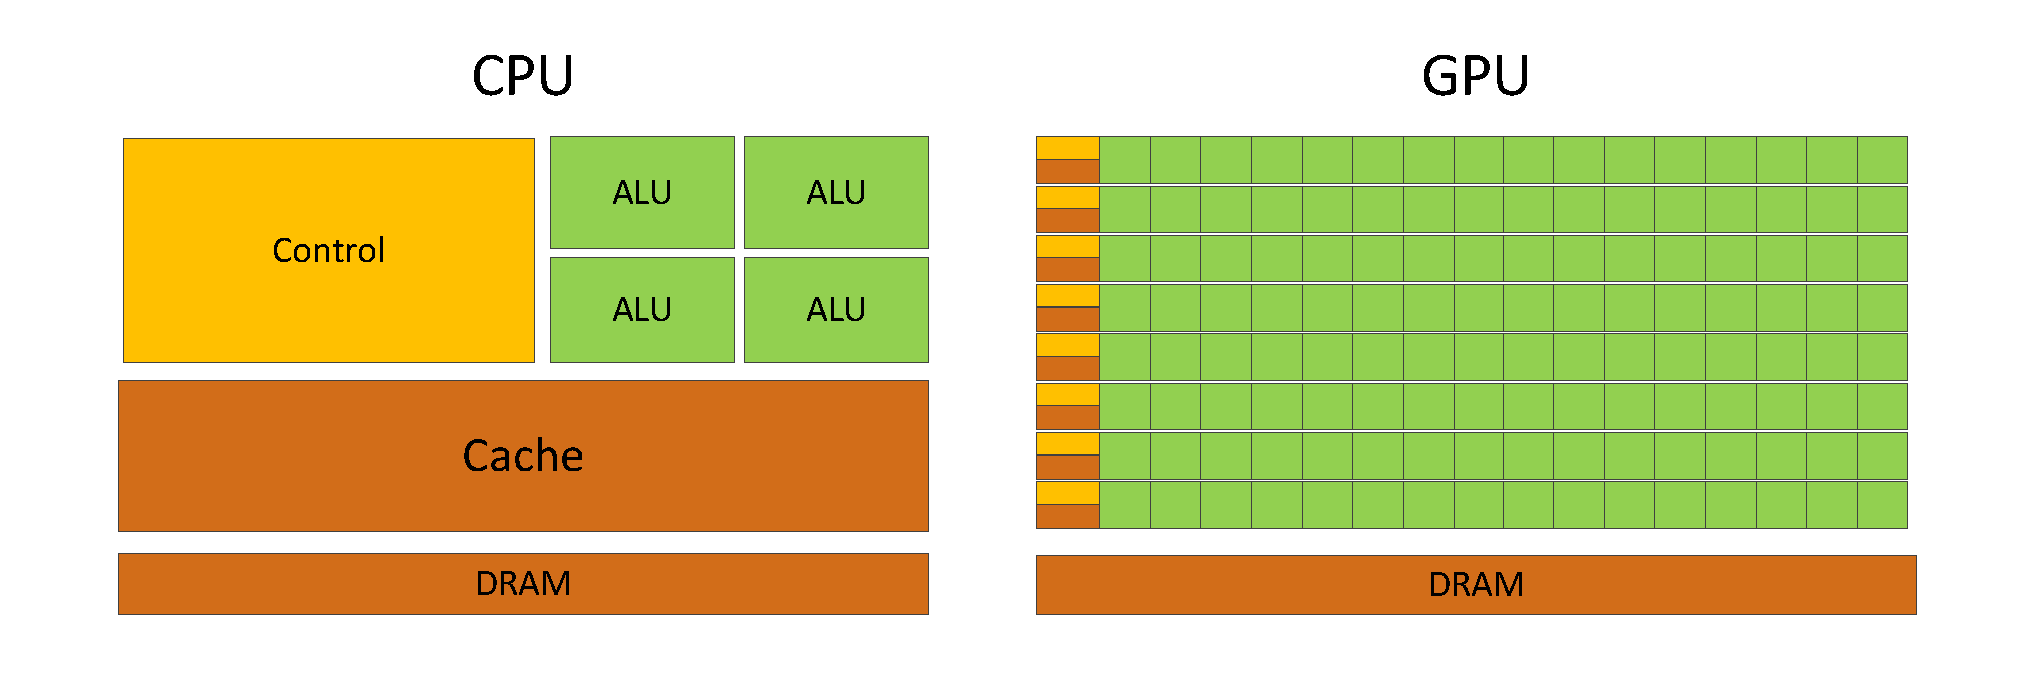
\includegraphics[width=1 \textwidth]{figures/GPU&CPU.pdf}}
\end{center}
\caption{{\footnotesize{GPU与CPU的区别}}}
\label{GCD}
\end{figure*}
\subsection{CPU与GPU区别}

图为 \ref{GCD} 为CPU和GPU的架构比较,可以看到,CPU和GPU的差异主要有两点:第一,GPU的ALU单元远远多于CPU;第二,GPU每个核心可用的逻辑控制单元和缓存相对CPU要少很多。CPU上大面积晶体管是逻辑控制单元和缓存单元,这是因为CPU的设计需要兼容多方面的应用,比如在桌面应用中就具有大量的分支控制操作和存储操作,而真正的数值计算操作却很少,所以CPU上具有大量的逻辑控制相关的实现,比如分支预测(Branch Prediction),乱序执行(Out Of Order execution)来满足这些分支控制需求,同时增加缓存大小来加速存储过程。但是这样的设计也使得留给CPU上的计算单元的晶体管面积较少,浮点计算能力较差,现在CPU为了弥补其计算能力的不足,产商常常在同块芯片上集成多个CPU核心,组成多核处理器,但是这样的设计并不能提高晶体管的利用率。

GPU最初被设计来进行图像渲染,图像渲染具有高度的并行性,而且大部分操作是浮点计算操作,逻辑控制较少,所以GPU在设计上采用简化控制单元,增加计算单元的设计思想,这使得在处理大规模浮点运算任务时,GPU的执行速度大大优于CPU的执行速度。
\subsection{CPU+GPU异构计算模型}
通过上面的分析,我们可以看到GPU适用于线程数目多,浮点计算密集和逻辑较简单的并行任务,而CPU更加适应于串行的分支较多,计算较少的任务。所以在实际中,常常把CPU和GPU结合起来,使用CPU和GPU两个部分协作共同完成并行计算任务。在这些并行任务中,CPU主要用于逻辑控制部分,而GPU 作为一种设备被CPU控制来做并行计算工作,这种协同工作模型被称为CPU+GPU 异构计算模型。
如图 \ref{GCY}所示为CPU+GPU异构计算结构示意图,GPU和CPU通过PCI总线进行连接,CPU调用GPU执行一共需要以下步骤:

1.把输入数据从CPU主机内存拷贝到GPU的内存(全局内存)中。

2.把执行程序加载到GPU上然后执行。

3.GPU上的程序在执行过程中需要从主存中读取数据,为了加快线程访问内存的速度,数据将通过多级缓存进行缓存。

4.GPU上程序执行完毕,将结果写在GPU主存中,这时需要将结果重新拷贝回CPU主机端进行处理。
\begin{figure*}
\setlength{\abovecaptionskip}{-0.5cm}
\begin{center}
{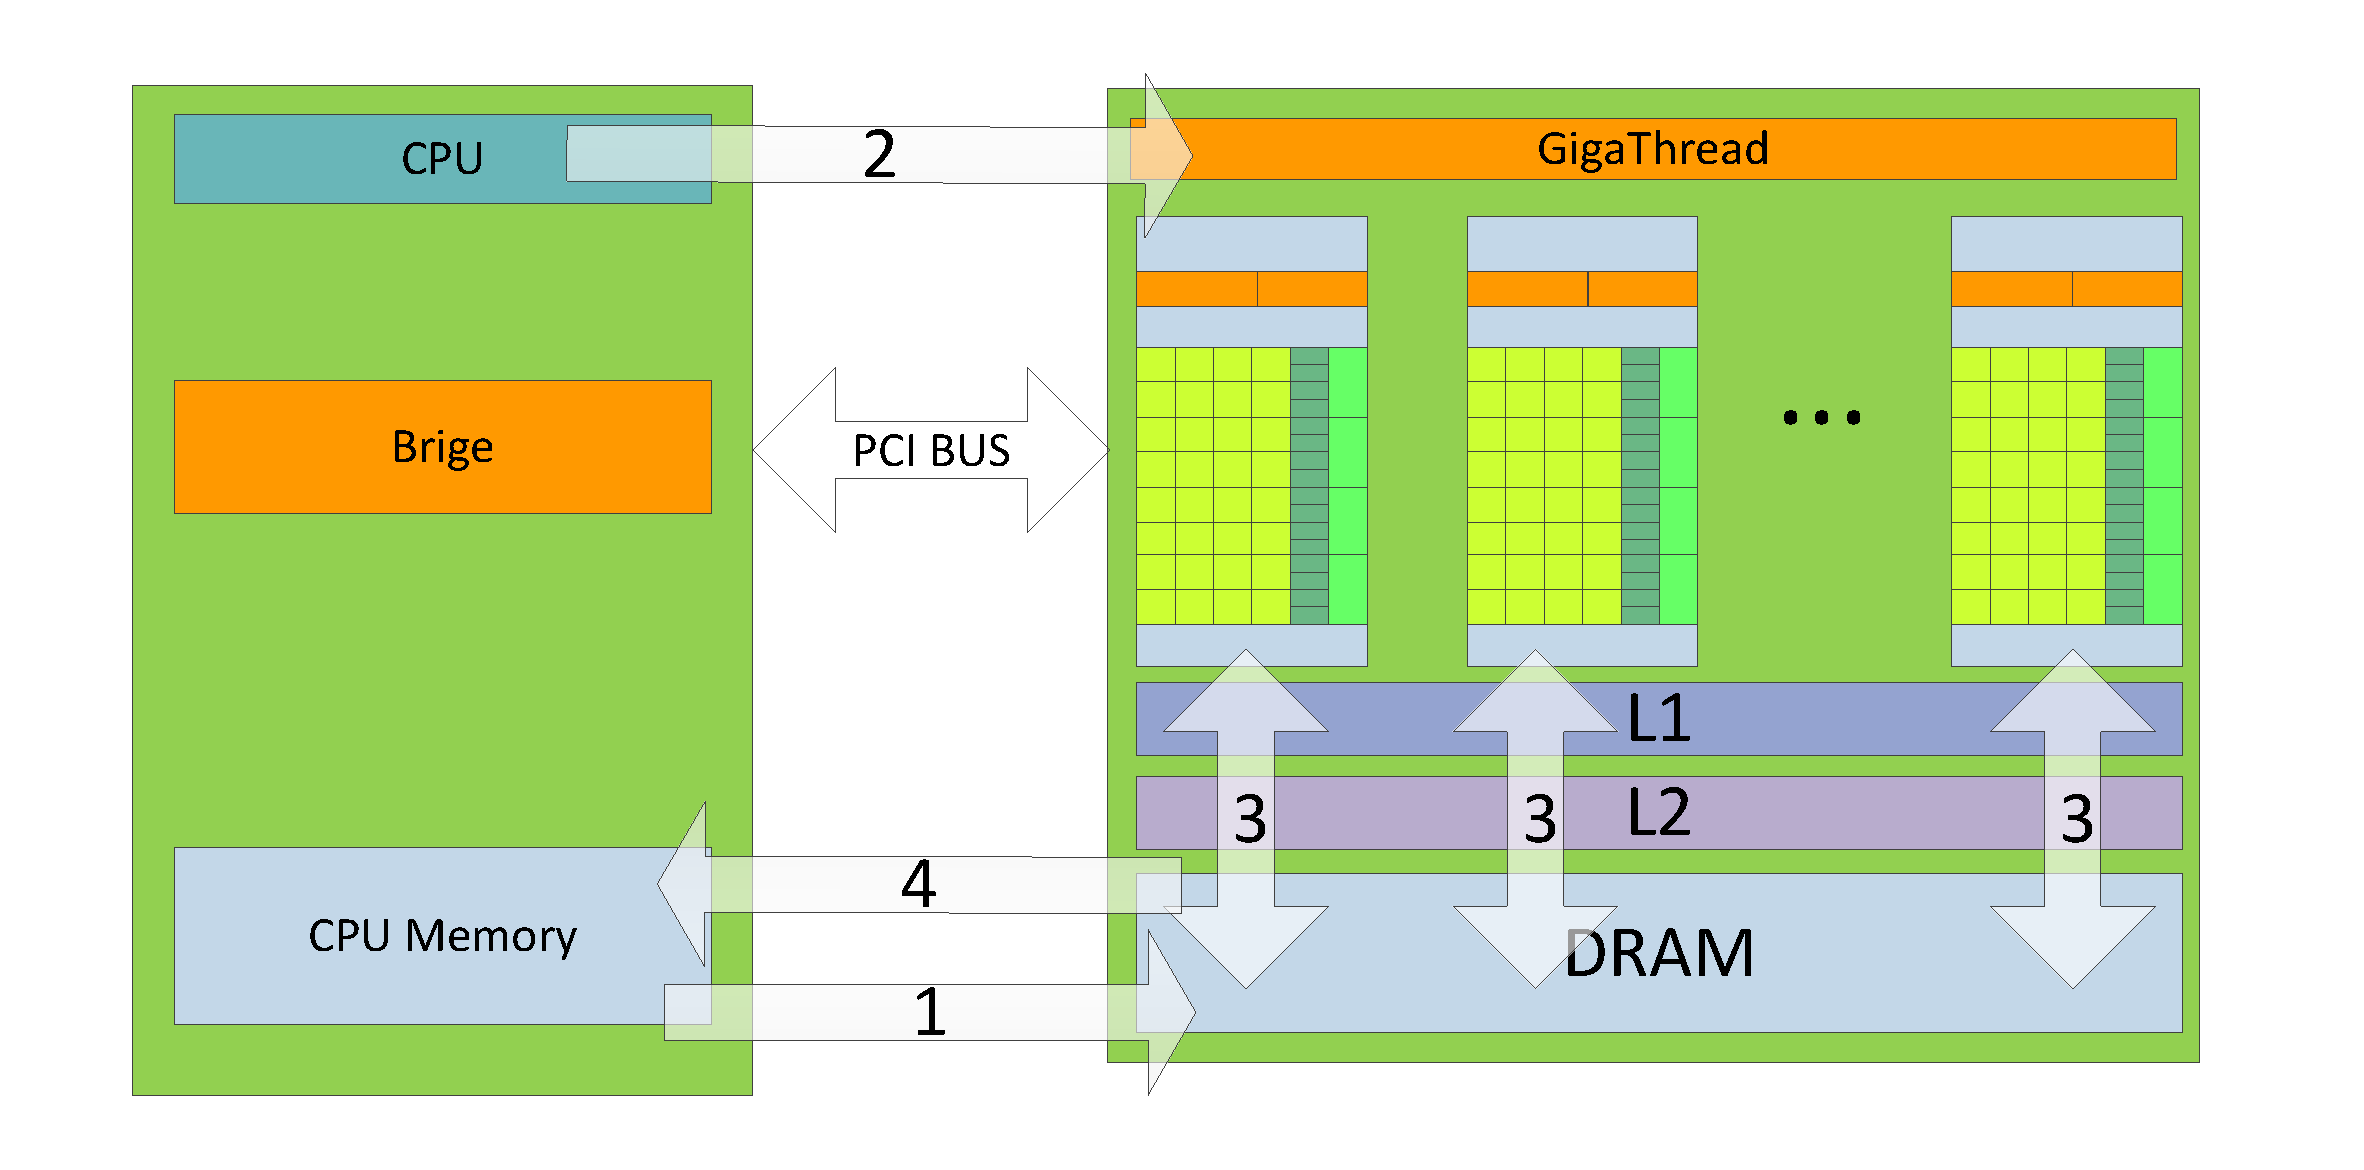
\includegraphics[width=0.8 \textwidth]{figures/yigou.pdf}}
\end{center}
\caption{{\footnotesize{GPU+CPU异构计算模型}}}
\label{GCY}
\end{figure*}
\section{GPU硬件架构}

虽然GPU相对于CPU在并行算法方面有很多优势,但是,由于GPU的出现是为了加速图形渲染问题,当想要使用GPU进行图形学之外的通用计算时,我们需要将问题转换为图形学问题,并且通过OpenGL或者DirectX等API来访问GPU,这对普通的开发人员提出了更高的要求,限制了GPU程序的设计自由度,使得GPU通用计算变得困难。2007年6月,NVIDIA推出CUDA (Compute Unified Device Architecture)\citing{CUDA}。CUDA简化了在GPU上的通用计算流程,使用CUDA进行并行算法设计,不需要把问题转化为图形学问题去调用图形学API,同时,CUDA采用类似于C语言的语言结构进行开发,这使得开发人员可以很快地熟悉和使用CUDA进行开发。但是,要设计出快速高效的CUDA程序,开发人员需要掌握GPU架构上的相关知识,利用GPU的特殊架构来优化算法的设计。

我们以NVIDIA Kepler架构为例子来介绍GPU的硬件架构。图 \ref{KPA} 为Kepler的GPU架构模型细节,Kepler架构包含两个部分,流处理器阵列(core 部分)和存储系统(memory)部分,Kepler架构中的GPU上一共包含15个流多处理器(SM),所有流多处理器共享一个L2缓存。
\begin{figure*}
\setlength{\abovecaptionskip}{-0.5cm}
\begin{center}
{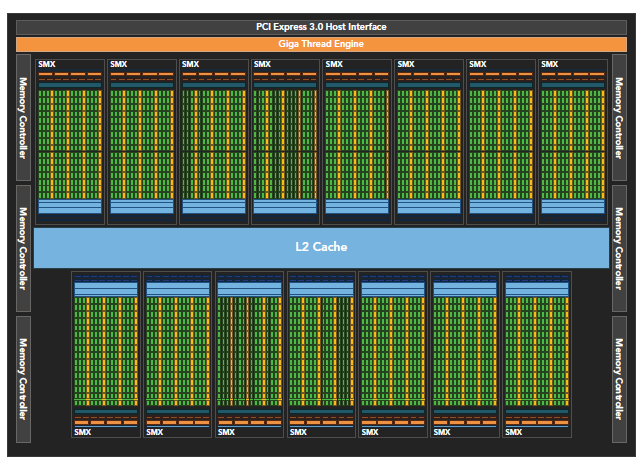
\includegraphics[width=1 \textwidth]{figures/arc.png}}
\end{center}
\caption{{\footnotesize{Kepler架构}}}
\label{KPA}
\end{figure*}
\subsection {流处理器}
我们看到GPU中主要组成部分是SM,一个SM(stream mutiprocessor)中含有大量的sp(stream processor),sp为GPU的计算核心,又称为流处理器,sp 是最基本的处理单元,指令和任务最终都是在sp上处理的,我们可以将在一个sp上执行的流看做一个独立的线程(thread),如果一个GPU中有更多的SM,一个SM中有更多的sp,那么就意味着这个GPU 在相同的时间内可以并行处理更多的任务。
\begin{figure*}
\setlength{\abovecaptionskip}{-0.5cm}
\begin{center}
{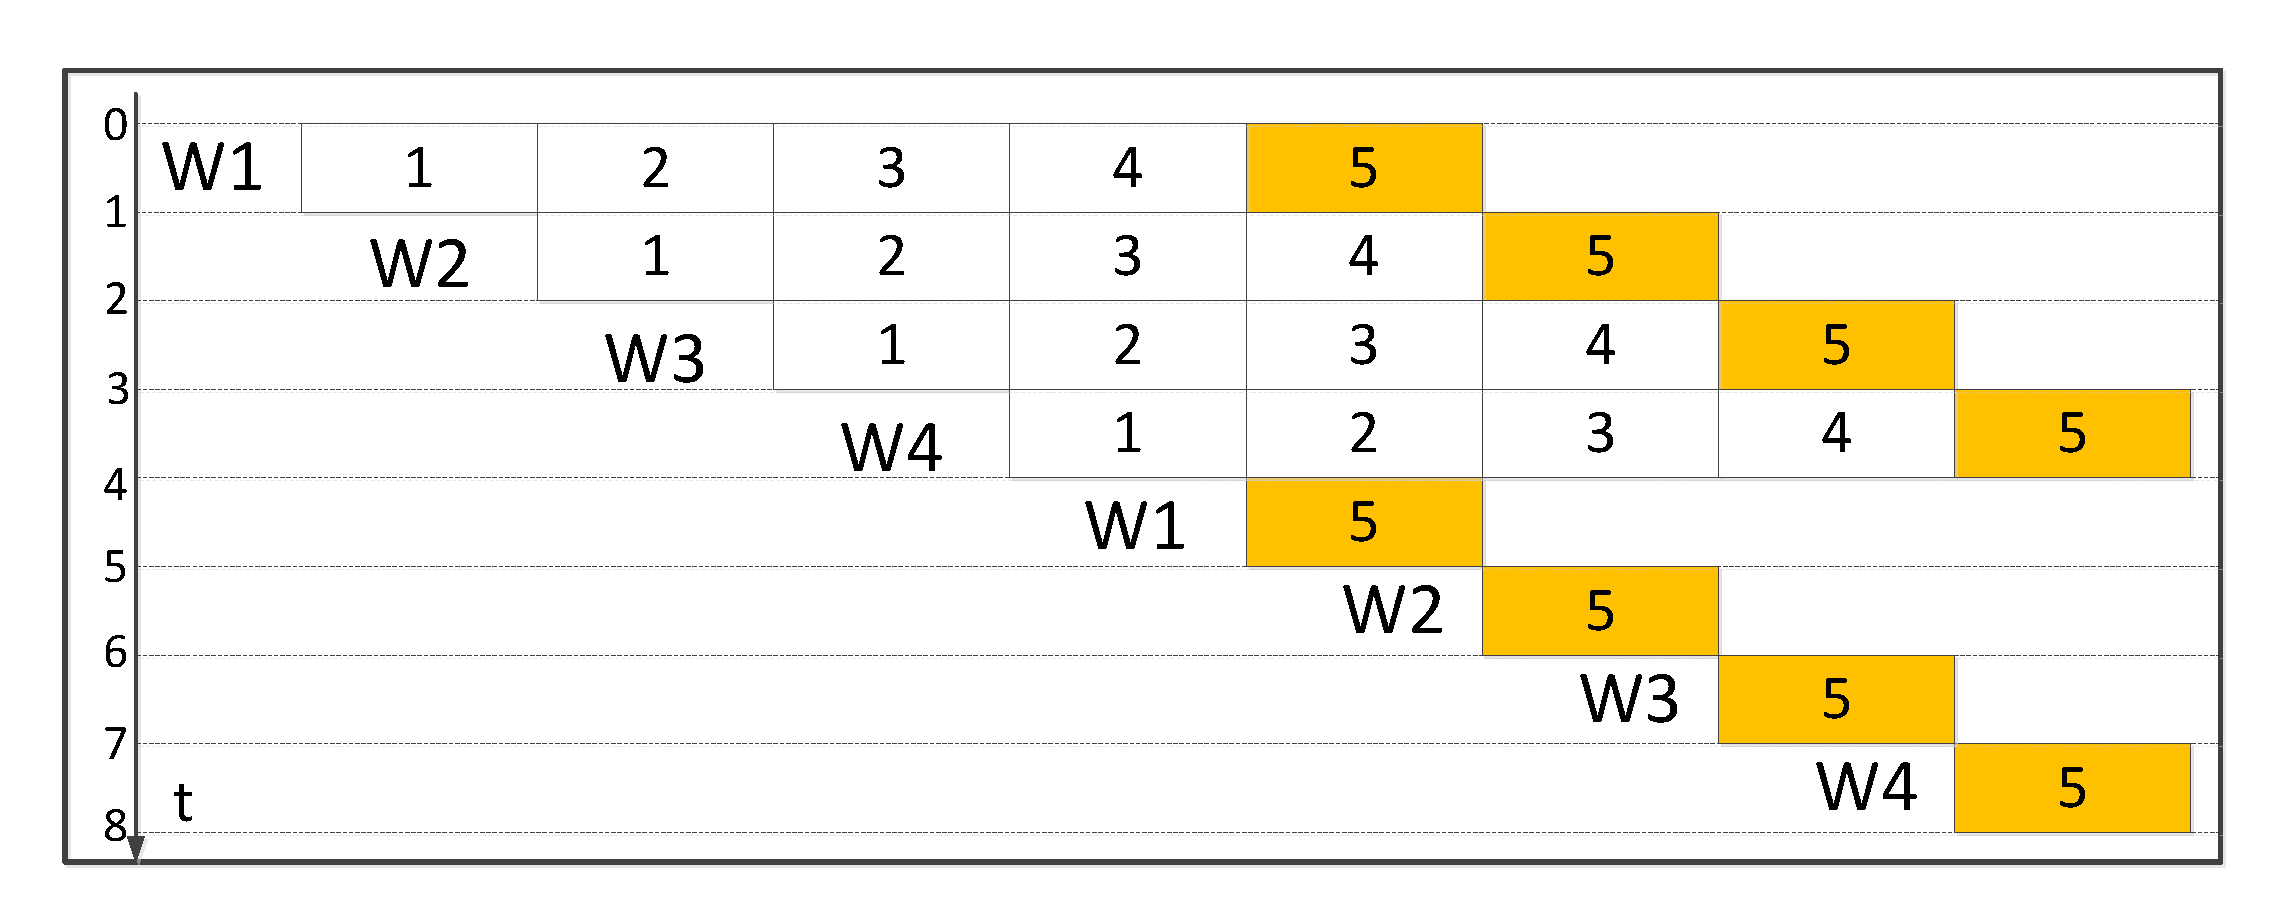
\includegraphics[width=0.8 \textwidth]{figures/warpsketch.pdf}}
\end{center}
\caption{{\footnotesize{warp切换示意图}}}
\label{wps}
\end{figure*}
\subsection{线程束(Wrap)}
warp是SM上线程调度和执行的单位,一个SM中的所有线程会被分成一个个warp组,通常一个warp组包含32个线程。同一个warp中的线程始终是同步的,这些线程都执行相同的指令,也就说同一个warp 中的线程必须等待所有线程都执行完了同一个指令后,才会去执行下一个指令。这样的设计虽然节省了硬件控制单元的复杂程度,但是也限制了GPU 在处理分支时的并行粒度,如果同一个warp 中的线程出现分支,每个线程执行的分支条件不一样,为了保持同步,不进入分支的空闲sp也必须等待进入分支的线程执行完毕后才能继续执行,这样使得sp 的利用率下降。

我们知道GPU 的浮点计算能力很强,但是在一些应用中常常需要进行内存的读写操作,这些访存操作会产生很长的时间延迟,从而限制了GPU的浮点计算吞吐量,为了充分利用GPU 上大规模的sp,GPU采用warp 切换来隐藏这些延迟。同一个SM上可以存在多个warp的程序上下文,但是同一时间只有一部分warp被执行。图 \ref{wps} 展示了warp上下文的切换过程,假设每个warp执行相同的代码,代码中需要先进行Load 操作,再进行计算操作,Load 操作需要等待4个时钟周期,而计算操作只需要使用一个时钟周期,W1-W4 表示4个不同的warp线程组。开始时W1先执行Load操作,而load 操作阻塞,这时warp调度器将W2调度到sp上进行执行,W2继续阻塞,直到第5个周期,W1的数据已经准备好了可以进行计算操作,当W1的计算操作结束后,继续切换计算W2,W3,W4。最终程序花费8个周期完成了对4个任务的计算,隐藏了12个周期的延迟,提高了sp的利用率。

\subsection{存储结构}
GPU中的每个SM中含有多种存储单元,包括寄存器,共享内存,常量内存,纹理内存。寄存器用来存储程序执行中的临时变量,同一个SM中的线程都能够访问共享内存,共享内存的访存速度大大高于主存的访存速度,所以在设计GPU并行代码时,我们常常先把频繁访问的数据提取到共享内存中,以减小延迟。另外,将中间结果存储在共享内存中,以减小对主存的访问,但是共享内存的大小是有限的,在Kepler架构中共享内存的大小为64KB。常量内存为只读内存,顾名思义它是用来缓存计算时需要的一些常量而专门设计的,常量内存大小为48KB。 纹理内存也是一种只读缓存,纹理内存是为图形学任务而设计的,在一些特殊的具有大量空间局部性的内存访问模式中能够提升性能并且减少内存流量。
\begin{figure*}
\setlength{\abovecaptionskip}{-0.5cm}
\begin{center}
{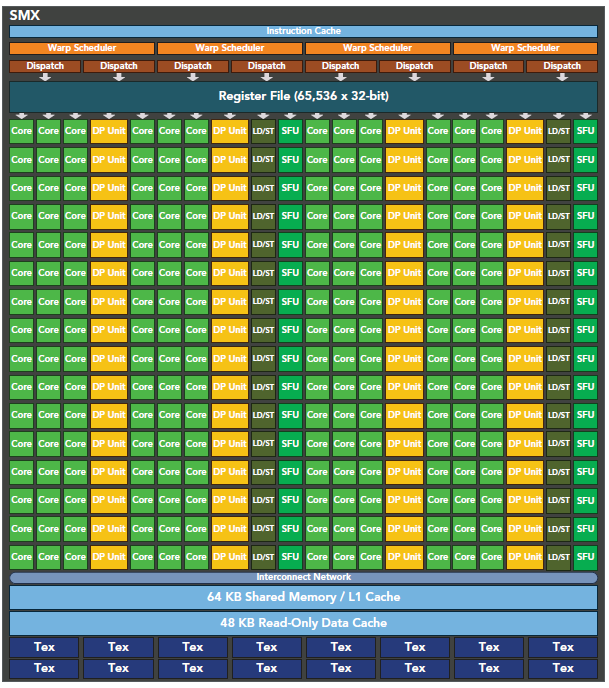
\includegraphics[width=0.8 \textwidth]{figures/smx.png}}
\end{center}
\caption{{\footnotesize{Kepler架构下的SM细节}}}
\label{sm}
\end{figure*}
\subsection{流多处理器细节}
Kepler架构下的SMX中包含192个单精度的CUDA core,64个双精度的单元(DP unit)和32个SFU(Special Function Unit, 特殊函数单元),32个存储(load/store)单元,其中SFU用来执行超越函数、插值以及其他特殊运算。Kepler架构下的GPU的每个SM包含了4个warp调度器和8个指令发射器。 Kepler架构下的每个SM可以同时调度64个warp共计2048个thread,而Kepler架构中一共有15个SM,也就是说,同一时刻最大可以支持30720个线程在GPU上调度执行,所以GPU的并行能力相当强大。
\begin{figure*}
\setlength{\abovecaptionskip}{-0.5cm}
\begin{center}
{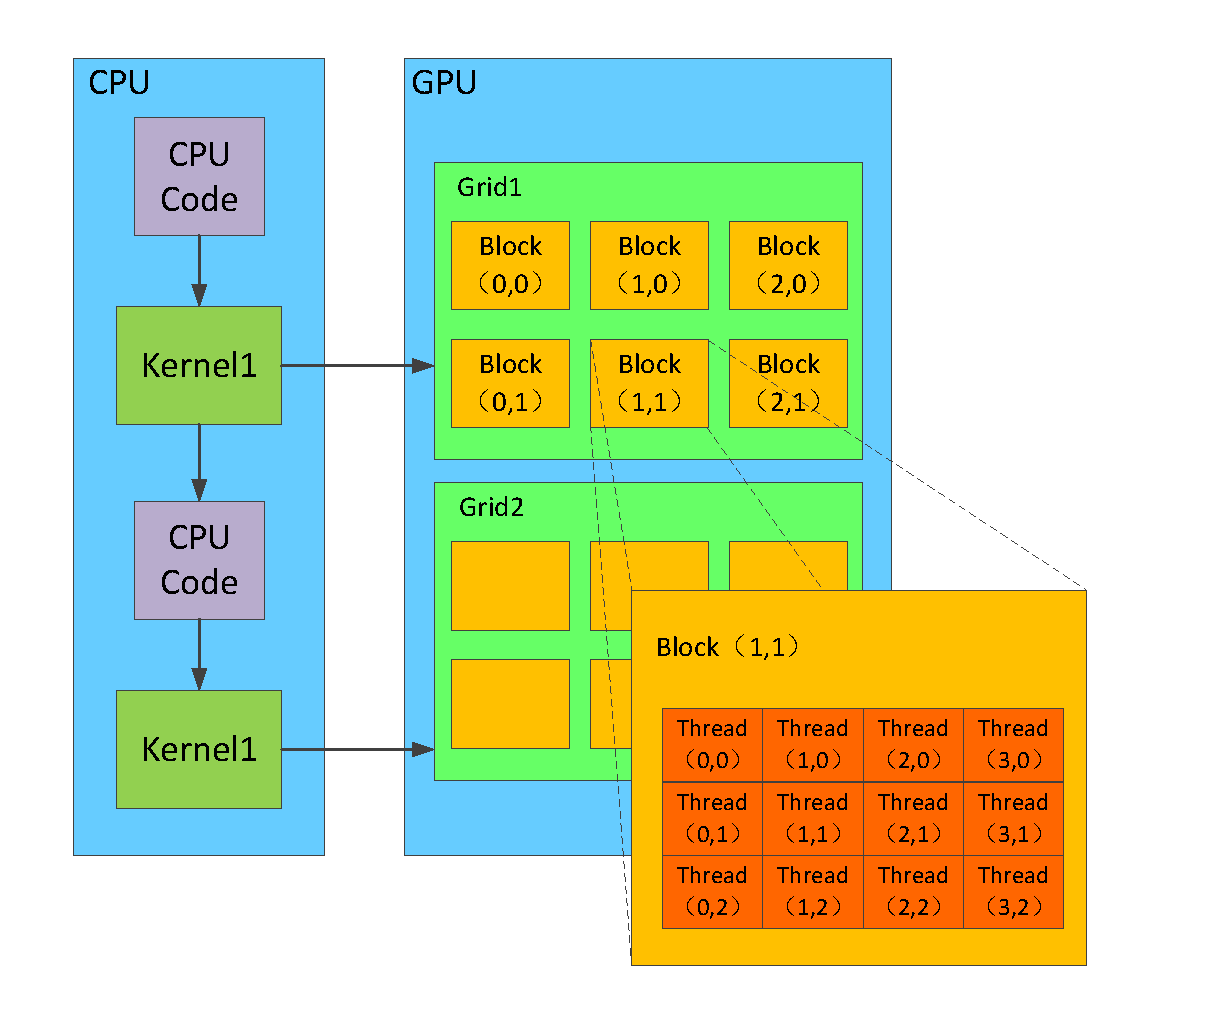
\includegraphics[width=0.7 \textwidth]{figures/block.pdf}}
\end{center}
\caption{{\footnotesize{CUDA异构执行流程和线程组织}}}
\label{ktz}
\end{figure*}
\subsection{执行模型}
GPU的执行模型被称为SIMT(Single Instruction ,Mutiple Thread),SIMT是对SIMD的一种改进\citing{CUDAR}。在CPU的SIMD中,向量宽带是受限的,在Intel 的SSE指令集中,假设一条SSE的指令宽带为128bit,那么它一次可以处理4个单精度浮点数,如果要用SSE指令处理一个单精度浮点数组,必须将数组打包成4个一组,然后才能把这些组交给CPU进行计算。但是在CUDA的模型中,我们为相同的指令产生不同的线程,这些线程的数量可以自由设置。在Kepler架构中,同一时刻GPU上可以调度执行30720个线程,这比CPU的SIMD的并行粒度高很多。

\section{CUDA编程模式}
CUDA是一种异构计算模型,CUDA程序在CPU和GPU上交互执行,CUDA的程序可以分为主机部分和设备部分,设备代码在一个或者多个GPU上执行,主机部分的代码在主机上执行,负责调度GPU上设备代码的执行。图 \ref{ktz} 展示了CUDA 异步执行流程,CPU通过调用kernel 函数来将代码发射到GPU上执行。

\subsection{CUDA软件线程组织}
一个CUDA程序包含大量并行执行的线程,在软件层面上,将多个线程组成一个block,同一个block中的线程又被分成不同的warp组,一个block中的线程只能在同一个SM中执行,同一个block中的线程可以通过调用同步函数(\_\_syncthreads())进行同步,同一个blcok中的线程可以共同访存shared\_memory,通过shared\_memory实现通信。一个kernel函数可以在软件层面上产生大量的线程,这些线程被组织成一个一个的block,如果SM足够,这些block中的线程将被加载到SM上调度执行,如果SM不足,block需要排队等待其他block完成执行。多个block组成一个Grid。block的维度可以是1-3维,图 \ref{ktz}展示了一个二维的block组织,每个block有自己的二维标号,同样每个block内部的线程也可以被组织成1-3维,图 \ref{ktz}展示了一个block内部的thread二维标号。

\subsection{kernel函数}
kernel函数是GPU上每个线程执行的函数,kernel函数在主机端调用,在GPU端执行,在调用kernel函数时需要为kernel函数设置一些参数,包括Grid维度大小和block维度大小。在kernel函数中使用blockIDx.x,blockIDx.y,blockIDx.z三个标号来访问当前block在Grid中的三维坐标,使用threadIDx.x,threadIDx.y,threadIDx.z三个标号来访问当前线程在block中的三维坐标。kernel函数中使用blockDim.x,blockDim.y,blockDim.z来表示block的三个维度的宽度。

\subsection{CUDA线程同步}
2.2.2介绍过同一个warp中的32个线程的执行是天然同步的,但是如果程序中存在更多的线程需求的话,我们就不能仅仅依赖于warp的性质进行同步,CUDA支持对同一个block中的所有线程进行同步,通过调用同步函数(\_\_syncthread()),一个block 中的线程可以实现同步,它表示block中所有的thread都要同步到这个点(\_\_syncthread()执行处)才能继续执行,这种同步操作相当于CPU上多线程的barrier(屏障)操作。GPU上线程同步的另一个问题是线程的写操作的同步问题,多个线程同时写相同地址的数据不是线程安全的。CUDA提供了一系列的原子操作来对多个线程间的共享数据的读写进行互斥保护,比如atomicAdd函数,他对目标地址的值进行原子加法操作,保证每次只有一个线程能对数据进行加法操作。
\begin{figure*}
\setlength{\abovecaptionskip}{-0.5cm}
\begin{center}
{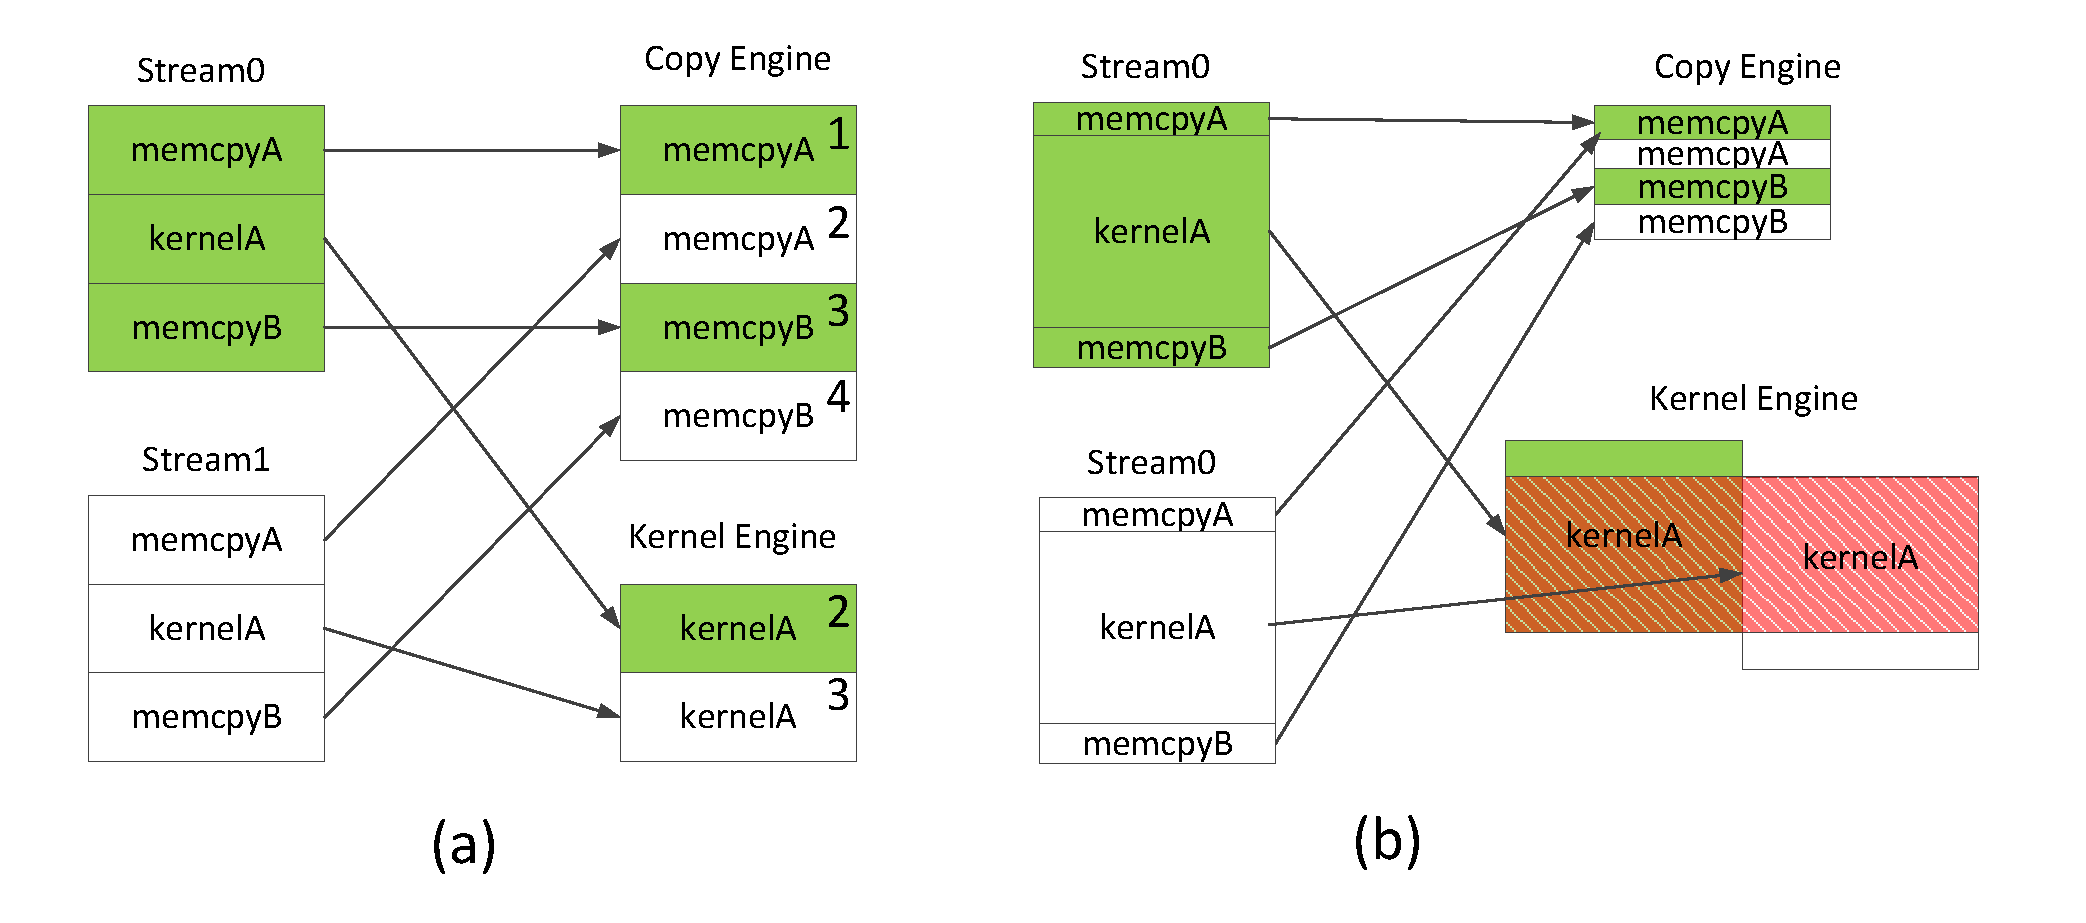
\includegraphics[width=1 \textwidth]{figures/flow.pdf}}
\end{center}
\caption{{\footnotesize{流并行示意图}}}
\label{flow}
\end{figure*}
\subsection{CUDA流并行}
CUDA程序通过流来管理并发,CUDA流代表一系列的GPU操作组成的队列,这些队列内部的操作按照顺序在GPU上执行,当我们调用kernel函数或者调用CUDA内部函数(cudamemcpy(),cudasyncthread()等)时,就是把一系列的GPU操作加到一个CUDA流队列中,这个流队列的操作会在GPU上按照加入的顺序执行。GPU上可以同时存在多个流队列,不同流之间的操作是无关的,流之间可以相互切换以充分利用GPU上的计算资源,虽然同一个流中的操作必须顺序执行,但是不同流之间的操作顺序是乱序的,而且还有可能是同时并行执行的,所以流并行也是GPU上的一个并行层次,我们可以把它视为任务上的并行,每个流代表了不同的任务,不同任务间的操作可以相互切换来隐藏延迟,从而提高了GPU的SM利用率,增大了并行粒度。同时,任务上的流并行,对编程人员来说是比较容易理解的,给GPU的并行代码设计带来了方便,我们可以为相似的任务设计相同的代码,通过流并行提高并行粒度,减小了设计难度。

我们观察图\ref{flow}中简单的流并行例子,来分析流并行的优势,图\ref{flow}中的Copy Engine表示GPU上的内存拷贝单元,负责和CPU端进行数据传输,Kernel Engine表示GPU上的kernel执行单元,负责kerenl的调度执行。在图 \ref{flow}(a) 中一共有两个流,两个流的操作相同,假设图中的每一个操作的执行时间相同,那么如果两个流串行执行,则总共需要6个时间单位,但是如果两个流相互切换,当Copy Engine在进行数据拷贝操作的同时,stream0的kernelA在Kernel Engine上执行,当stream0的kernelA执行完毕后,stream1的kernelA也已经准备好可以执行了,这样Copy Engine的数据传输带宽和GPU的计算带宽都得到充分利用,一共只需要4个时间单位,就可以完成两个流的操作。图 \ref{flow}(b) 中,假设两个流的数据拷贝操作所占用的时间比较少,而kernel需要的计算时间较长,这个时候由于两个流的kernel都会很快准备好发射,如果SM资源足够,两个kernel将同时在GPU上调度执行,如图\ref{flow}(b)中的红色部分表示重叠执行的时间,可以看到这种情况下多个流的并行可以大大节省运算时间,充分利用SM资源。

\section{本章总结}
本章简略介绍了GPU的体系架构和CUDA编程框架,说明了GPU的的强大计算能力和一些GPU程序设计上需要注意的问题,为后面的第三、四章介绍做铺垫。

% !Mode:: "TeX:UTF-8"
\chapter{SDN IP网络下的并行业务量工程算法研究}
\section{引言}
SDN IP网络中的业务量工程问题可以被建模成一个多商品流问题,将网络业务作为问题的输入,寻找最优的路由来最小化代价函数。代价函数通常被设置为对网络拥塞程度的评价水平,比如,最常用的代价函数是最大链路利用率(MLU),简单地被定义为利用率最高的那条链路的链路利用率 \citing{MLU1, MLU2},另外一些文献 \citing{Convex1, Convex2}把所有链路的链路利用率的和作为代价函数,链路利用率代价函数的逻辑是:(1)低链路利用率意味着低的网络延迟。(2)维持低的链路利用率意味着预留更多的空间给其他将来到达的业务。但是大量基于实际拓扑的实验表明链路利用率代价函数,特别是MLU,在网络利用率没有达到拥塞程度的时候,不是对网络优化的较好评价函数 \citing{BeyondMLU}。在这个实验\citing{BeyondMLU}中,当链路利用率低于0.9的时候会造成不可忽略的网络性能中断。反之,在网络发生大量拥塞的情况下,MLU只去优化最大的链路利用率,而不能给出一个可行(满足容量约束)的解。所以作为替代,本文采用路由代价作为代价函数,我们假设已经知道短时间内到达的一批业务,控制器需要计算出满足链路容量约束的路径,并且最小化总的路由代价。为了使得加入网络的业务尽量多,我们设定被阻塞的业务的代价为一个较大值。

本章主要设计了两种业务量工程算法,第一种是基于备选路径模型的业务量工程算法,采用遗传算法来优化目标函数,并且设计了遗传算法的并行版本。第二种是基于拉格朗日松弛的优化算法,算法把链路容量约束松弛到目标函数,并把业务量工程问题分解成一批业务的路由计算问题,从而采用GPU进行并行计算。
\section{网络模型和问题建模}
\subsection{网络模型}

本文将SDN网络建模成有向图 $G(V, E)$,$V$表示所有的点集合,$E$是所有边的集合, $n = |V|$ 和 $m = |E|$ 分别表示点数和边数。对每一条边$(i,j)\in E$, $w_{ij}$ 表示此边 $(i,j)$上的权重(传输一单位的流量需要的代价),不失一般性,我们假设每条链路上的$w_{ij}$是整数,对每一条边 $(i,j)$, $c_{ij}$表示此边上的容量,假设$D$表示需要被路由的业务需求集合,业务$d \in D$ 是一个元组 $(s_d, t_d, bw_d)$,其中, $s_d$表示业务的源节点,$t_d$表示业务的目的节点,$bw_d$表示业务d需要的流量带宽。
\subsection{问题建模}
本小节,我们把业务量工程问题建模成一个混合整数规划模型(MILP),本文采用新的代价函数,如下式\ref{Obj1},\ref{obin}:
\begin{equation}\label{Obj1}
\sum\limits_{d \in D} f(\mathbf{d})
\end{equation}
\begin{equation}\label{obin}
f(\mathbf{d})=\begin{cases}
c(p_d) \cdot bw_{d} & \text{如果业务可以被加入}\\
W \cdot bw_{d}& \text{如果业务被阻塞}
\end{cases}
\end{equation}
其中$p_d$是计算出来的对应于业务$d$的路径,$c(p_d)$ ($c(p_d) = \sum_{(i,j)\in p_d} w_{ij}$) 表示的是此路径$p_d$ 的代价,$W$为一个较大的值,比如$W$远远大于业务所有可能的路径代价值。因为不知道带宽是否足够容纳所有业务,\ref{Obj1}有两个分支,为了使得表达式同一,方便表示,
我们首先构建辅助图$G_a(V_a, E_a)$ ,对每个点$v \in V$和$u \in V$,在$G_a(V_a,E_a)$中添加一条链路$(v,u)$,并且设置链路 $(u,v)$ 的容量和代价分别为$\infty$和$W$。然后,我们把$G_a(V_a,E_a)$和原图$G(V,E)$合并成一个新图$G_b(V_b,E_b)$,那么图$G_b(V_b,E_b)$就有足够的容量来容纳业务需求,如果某条业务被路由到$G_a(V_a, E_a)$的链路上,那么就表示这条业务被阻塞了,构建了辅助图$G_b(V_b, E_b)$后,业务量工程问题的代价函数可以表示为:
\begin{equation}\label{Obj2}
z^* = minimize~f(\mathbf{d})=
\sum\limits_{d \in D} c(p_d)\cdot bw_d= \sum\limits_{d \in D}\sum\limits_{e \in p_d} w_e \cdot bw_d
\end{equation}
在本文的业务量工程问题中,每个业务只能够路由到一条路径上,如第二章中讨论的那样,这更符合于SDN网络的实际情况,以下整数约束能够保证每个业务只走一条路径
\begin{equation}\label{FlowConv}
\begin{split}
\sum\limits_{(i,j) \in E_b} x_{ij}^d - \sum\limits_{(j,i) \in E_b} x_{ji}^d
=\begin{cases}
1 & \text{if $i = s_d$}\\
-1 & \text{if $i = t_d$} \\
0 &{otherwise}
\end{cases}
\\~~~~~~~~\forall i\in V_a, \forall d\in D
\end{split}
\end{equation}
\vspace{-0.4cm}
其中 $x_{ij}^d$是一个01整数变量, $x_{ij}^d=1$表示业务$d$的路由经过了链路$(i,j)$,为了避免链路拥塞,路由需要满足以下的链路容量约束:
\begin{equation}\label{Capcon}
\sum\limits_{d \in D}x_{ij}^d \cdot bw_d \le c_{ij} ~~\forall (i,j)\in E_b
\end{equation}
在这个模型中,变量的数量随着业务量大小和网络规模大小呈倍数增长,所以这个MILP模型在大规模情况下很难求解。
\section{基于遗传算法的业务量工程算法}
\subsection{备选路模型}
模型(\ref{Obj2},\ref{FlowConv},\ref{Capcon})的一种常见的简化模型被称为基于备选路径的模型\citing{multi-commodity},在备选路径模型中,为每一个业务$d \in D$,预先产生了$K$条不同的路径作为备选路径集合$P_d=\{p^1_d,p^2_d,p^3_d...p^K_d\}$,通过在这些备选路径中进行选择来优化目标函数\ref{Obj2},
为了表示业务被阻塞的情况,我们在业务的备选路径集合$P_d$中添加一条路径$p^0_d$,$p_d^0$是图$G_a(V_a,E_a)$上的路由,其代价为$W$,所经过的链路容量为$\infty$。于是,模型可以被描述如下:
\begin{equation}\label{Obj3}
z^* = minimize~f(\mathbf{d})=
\sum\limits_{k \in [0,K]}\sum\limits_{d \in D} c(p_d^k)\cdot x_k^d\cdot bw_d
\end{equation}
\begin{equation}\label{Cons1}
\sum\limits_{k \in [0,K]}x_k^d=1
\end{equation}
\begin{equation}\label{Cons2}
\sum\limits_{k \in [0,K]}\sum\limits_{d \in D} y_{ijk}^d\cdot x_k^d\cdot bw_d\le c_{ij} ~~\forall (i,j)\in E_b
\end{equation}
其中,$x_k^d$为一个01变量,当$x_k^d=1$时表示业务d选择其备选路径中的第k条路径,$y_{ijk}^d$是一个01变量,$y_{ijk}^d=1$表示业务$d$的第$k$条路径经过了链路$(i,j)$。约束\ref{Cons1}表示每个业务只能选择一条路径,约束\ref{Cons2}表示经过链路上的总流量大小不能超过链路上的容量大小。在这个模型中,由于我们把业务的路径限制在其备选路径集合中,所以他的变量个数比模型(\ref{Obj2},\ref{FlowConv},\ref{Capcon})要少很多,本节将通过遗传算法来求解这个简化的模型,设计出基于遗传算法的并行业务量工程算法GA-PTEA(Genetic Algorithm Based Parallel Traffic Engineering Algorithm)。

\subsection{遗传算法设计}
遗传算法是一种模拟自然进化过程来搜索问题最优解的启发式算法。遗传算法模仿达尔文进化论和自然选择过程来评价挑选最优解集合,遗传算法从一个代表问题的可行解的种群出发,一个种群中不同个体代表了不同的解,每个个体实际上是一个染色体,染色体携带表达当前解的信息编码,初代种群产生后,对每个染色体个体进行评价,按照适者生存,优胜劣汰的原则,使得优秀的个体更有可能把自己的遗传信息传递给下一代,从而得到更优秀的后代。在遗传算法的迭代过程中,一部分基因会发生变异,好的变异能够提高解的质量,增加算法的搜索空间,避免算法收敛于局部最优解。遗传算法的算法流程图如图\ref{IterNum} 所示,遗传算法先从初始种群开始,循环的地进行交叉,变异,评价选优这三种操作,最终得到一个最优秀的个体作为问题的解。
\begin{figure}
\setlength{\abovecaptionskip}{-0.5cm}
\begin{center}
{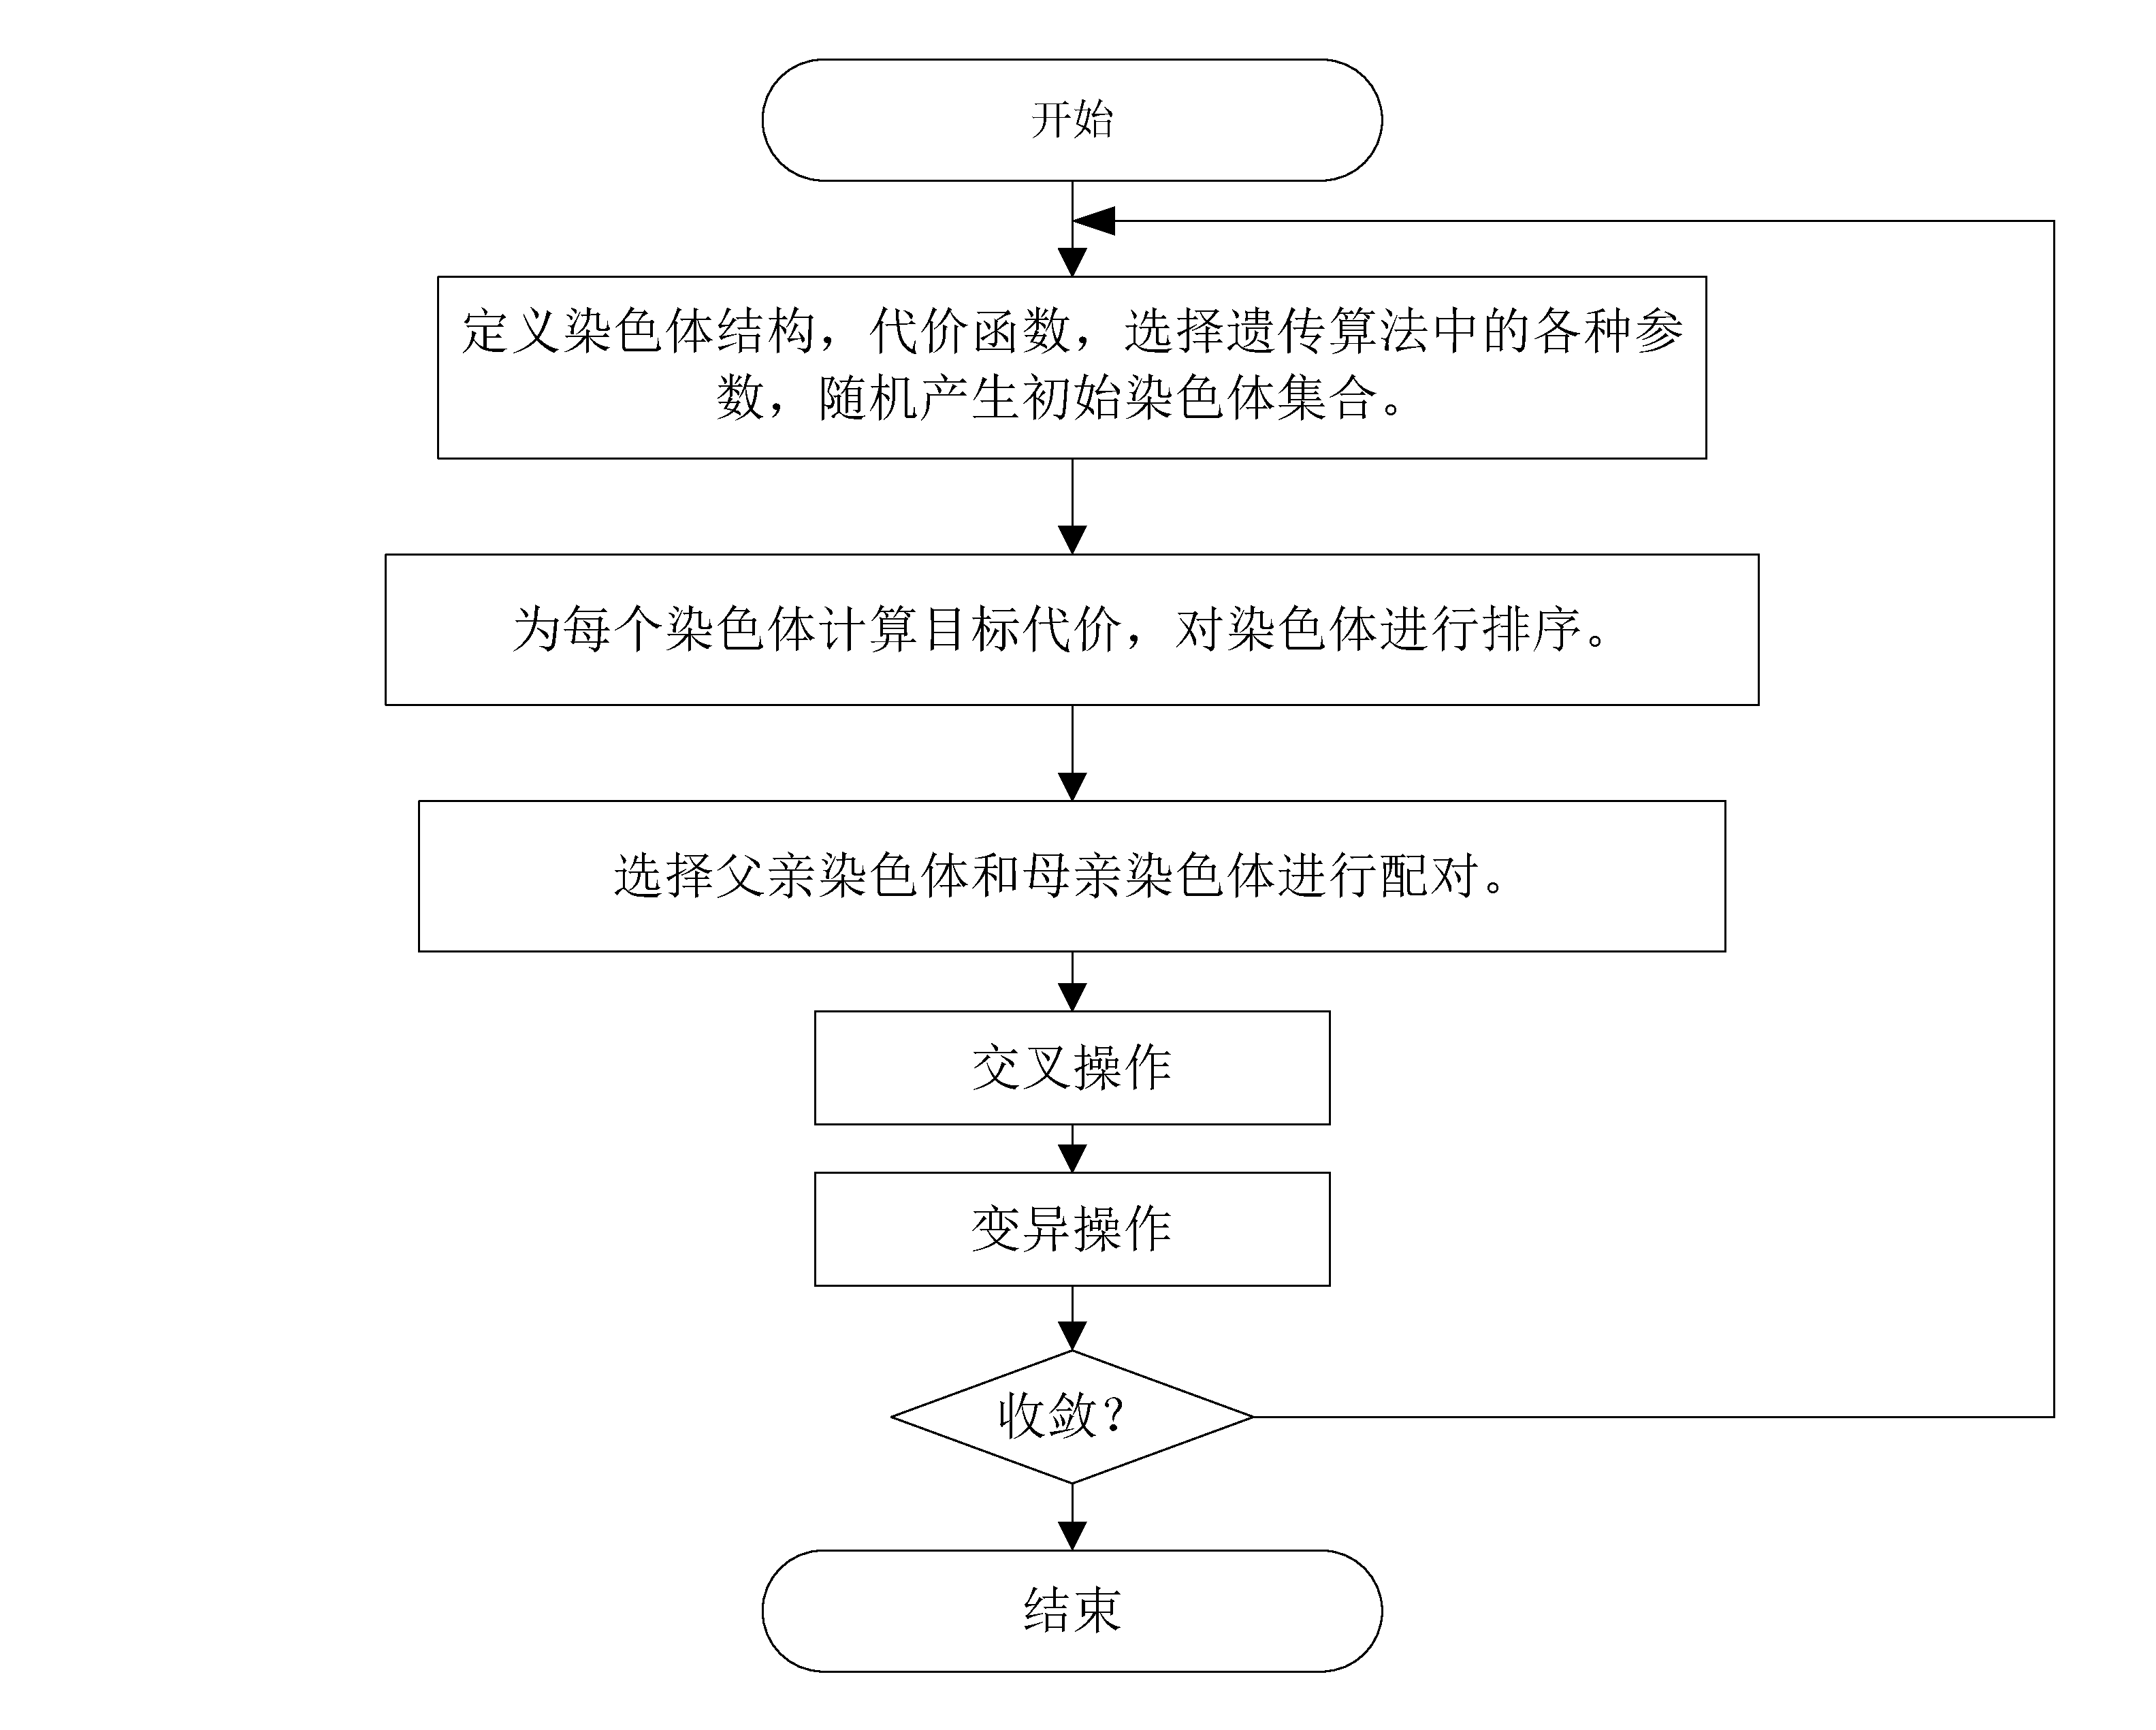
\includegraphics[width=0.8 \textwidth]{figures/GAprocess.pdf}}
\end{center}
\caption{{\footnotesize{遗传算法流程图}}}
\label{IterNum}
\end{figure}
\subsubsection{染色体结构}

假设业务数量为$|D|$,初始染色体集合大小为$POP$,集合$C$表示染色体种群集合,$C_j$表示第$j$($j \in [1,POP]$)号染色体,$C^i_j=k,(k \in [1,K])$表示在第$j$号染色体中,业务$i$选择了第$k$条备选路径,$C^i_j=0$表示业务$i$被阻塞(在辅助图$G_a(V_a,E_a)$上路由)。$|p^i_d|$表示业务$d$的第$i$ 条备选路的路由代价,$rp^i_d$ 表示路径$p^i_d$ 上的最小可用容量,$rp^i_d=min(r_e|e \in p^i_d)$,其中$e \in p^i_d$ 表示路径$p^i_d$上的边,$r_e$ 表示此边$e$ 上的剩余容量。
\subsubsection{初始可行解的生成}
可行解表示满足容量约束的解,为了使得遗传算法有效,初始解的质量很重要,产生的初始解要尽量好,这表示要有更多的业务被加入到网络中,而且保证业务的路由代价较小,本文采用一种简单的贪心算法来产生出初始可行解,如算法\ref{alg:Framwork}所示:
\begin{algorithm}[htb]
\begin{algorithmic}[1]
\Require{$G(v,E)$:网络拓扑;$P$:备选路径集合;$C$:未初始化的染色体集合;}
\Ensure{$C$:可行染色体集合;}
\For{$c_j \in C$}
\For{$c^d_j \in c_j$ }
\State {$c^d_j\leftarrow k^d_j$,其中$k^d_j$为$1$到$K$之间的随机值,随机选择一条备选路}
\EndFor
\State {对染色体中的的每个业务需求按照值$\frac{\sqrt{bw_d}}{|p^{k^d_j}_d|}$}进行降序排序。
\For{$c^d_j \in c_j$ }
\If{$rp^{k^d_j}_d \ge bw_d$}
\State 加入路径$p^{k^d_j}_d$到网络,更新网络链路容量。
\Else
\State {$c^d_j \leftarrow 0$}
\EndIf
\EndFor
\EndFor
\end{algorithmic}
\caption{初始可行解生成算法}
\label{alg:Framwork}
\end{algorithm}

对每一个染色体,算法\ref{alg:Framwork}随机地为每个业务选择备选路径标号,但是这样选择出来的路径集合有可能会超过网络链路的容量限制,从而使得解变得不可行,要得到可行解,必须从解中剔除一部分业务。使得他们阻塞,本文使用一种启发式策略来确定需要剔除的业务。一方面,要使得目标函数变小,那些流量需求较大的业务应该优先被加入到网络中。但是,另一方面,如果大流量的业务的路由代价很大,经过了一条很长的路径,就会大量地浪费网络中的链路容量资源。所以算法对当前染色体$j$中的业务和其路径按照$\frac{\sqrt{bw_d}}{|p^{k^d_j}_d|}$ 的值进行排序,其中${bw_d}$ 代表当前业务$d$所需要的流量大小,$|p^{k^d_j}_d|$代表集合$P_d$ 中的第${k^d_j}$条路径的代价大小,观察目标函数,目标函数是最小化路由代价,而$\frac{\sqrt{bw_d}}{|p^{k^d_j}_d|}$较大意味着较大的流量经过较小代价的链路进行路由,这种路由是很理想的,尽量节省网络的链路使用资源的同时,又减小了总体目标函数,所以这个比例值是对业务路由优劣程度的较好评价。算法按照比例值排序的结果依次尝试将路径$p^{k^d_j}_d$加入到网络中,如果$rp^{k^d_j}_d \ge bw_d$,表示路由经过的链路有足够的容量来容纳这一业务,所以加入业务到网络中,并且更新网络的链路容量大小,反之,如果$rp^{k^d_j}_d<bw_d$,这个业务选择这一条路径会超过网络链路的容量限制,于是这条业务被阻塞,染色体中的相应基因位置被设置为0。算法\ref{alg:Framwork}结束后我们便可以得到一个可行的染色体,我们多次运行算法\ref{alg:Framwork}就可以得到一个初始可行染色体集合$C$。

\subsubsection{评价与排序}

评价过程对每一个染色体计算其相应的目标代价函数值,由于遗传算法中的交叉和变异步骤可能会产生不可行的染色体解(链路容量超限),我们把这样的染色体评价为一个很大的代价(INF),从而在选优时被排除掉。染色体评价完成后,我们把染色体按照代价函数值进行降序排序,我们把排序好的染色体分为三组:

精英染色体集合:目标值排在最前面的$\alpha$个染色体构成精英染色体集合$A$,精英染色体将直接保留到下一轮迭代,而且精英染色体可以产生后代。

次优染色体集合:精英染色体后的$\beta$个染色体构成次优染色体集合$B$,次优染色体集合中的染色体不会直接保留到下一轮,但是他们可以和精英染色体进行交叉产生后代。

劣等染色体集合:最后剩余的$\gamma$个染色体构成劣等染色体集合$G$,由于其代价函数值一般较大,其选路策略不可取,算法直接扔掉这一部分劣等染色体,不允许劣等染色体产生后代。
\subsubsection{交叉}
交叉过程从精英染色体集合$A$中随机地选取一个染色体$c_i \in A$作为父亲,从精英染色体集合和较优染色体集合的并集$A \cup B$ 中随机选取一个染色体$c_j \in A \cup B$ 作为母亲,将$c_i$ 和$c_j$进行均匀交叉得到新的染色体$s$。均匀交叉的过程是,对$s$的每一个基因点位以$\%50$的几率选择继承父亲或者母亲的相应点位的路径选择。重复以上过程$\beta$ 次,从而产生$\beta$个新的子染色体。
\subsubsection{变异}
变异过程采用随机变异,随机在集合$A \cup B$中选取$\gamma$条染色体,对某一选定的染色体$c_j \in A \cup B$,随机选取$m$个业务基因点位,进行变异,将当前已经选择的路径编号随机改变为备选路集合中的另外一个值,变异过程能够提高算法的的搜索空间,避免算法陷入局部最优解。
\subsubsection{终止条件}
假设第前$k$次迭代找到的最优解为$B^*$,第k+1次迭代找到最优解为$b_{k+1}^*$,如果$b_{k+1}^*<B^*$,那么就更新$B^*=b_{k+1}^*$,如果连续迭代$L$次,$B^*$都不被更新,则判定算法收敛,算法停止。
\subsection{基于GPU的并行遗传算法设计}
\subsubsection{并行评价算法设计}
\begin{figure}
\setlength{\abovecaptionskip}{-0.5cm}
\begin{center}
{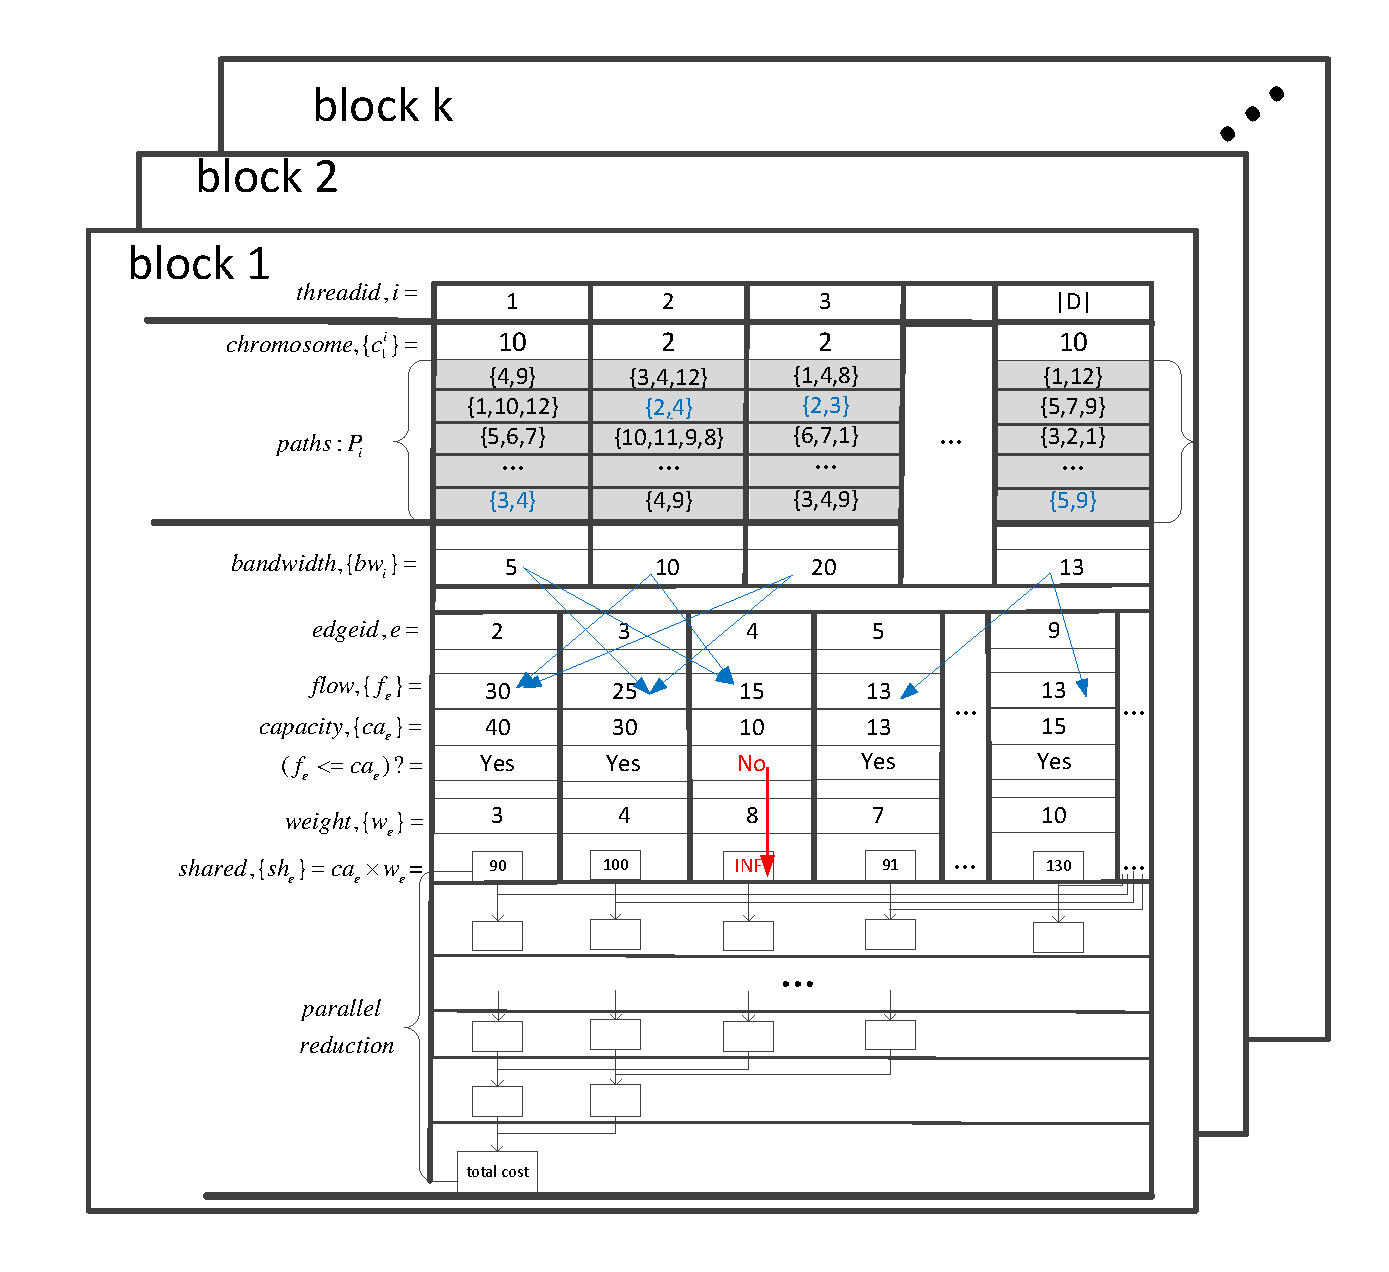
\includegraphics[width=1 \textwidth]{figures/GPUfitness.pdf}}
\end{center}
\caption{{\footnotesize{GPU并行评价示例}}}
\label{fitness}
\end{figure}
遗传算法中最消耗时间的部分是染色体评价部分,由于需要评价大量的染色体,评价每个染色体都需要大量的计算开销。但是幸运的是遗传算法具有天然的并行性,每个不同的染色体评价可以并行执行,更进一步,每个染色体中的不同基因的计算也可以并行执行,这样并行粒度是达到$|POP|\times|D|$。在具体介绍并行算法之前,我们先引入一些符号,如下:

染色体相关符号:$C$表示染色体种群集合,$c_j$表示第$j$个染色体,$c^d_i$表示第$i$个染色体的第$d$个基因位置。

备选路径相关符号:$P$为所有业务的备选路径组成的集合,$P_i$表示业务$i$的所有备选路径集合,$p_i^k \in P_i$表示集合$P_i$中的第$k$条路径。

业务带宽数组$bw$,$bw_i$表示第$i$个业务需要的带宽大小。

链路流量数组$f$,$f_e$表示链路$e$上总的流量大小。

链路单位代价数组$w$,$w_e$表示链路$e$上的单位代价(流过一单位的流量所需要的代价)。

链路容量数组$ca$,$ca_e$表示链路$e$上的容量大小。

链路代价数组$sh$,$sh_e$表示链路$e$上总的路由代价。

目标函数值数组$ob$,$ob_j$表示第$j$个染色体对应的目标函数值。

由于每个染色体的计算过程是独立的,算法为每一个染色体开辟一个block,一个block内部的第$d$号线程负责当前染色体上第$d$号业务的计算。算法 \ref{evaluate}展示了负责评价的kernel函数evaluate,算法一共可以分为两个部分:

第一,流量统计部分(2-9行):算法需要对染色体进行可行性判断,也就是判断是否有链路的流量大小超过其容量大小,为此,算法需要统计每一条边上的流量大小,我们在共享内存中开辟数组$f$用以统计流量,$f$数组被初始化为0。一个block中的每一个线程首先通过寻址备选路径集合找到业务选择的路径,
业务每经过一条链路都需要占用该链路上的容量,所以如果路径经过了链路$e$,$f_e$就需要被加上此业务的流量大小。block中的每一个线程都会遍历业务所选择的路径,对$f$数组进行加法操作,但是多个线程可能同时对$f$数组中的同一个地址进行加法操作,这不是同步安全的,所以算法使用atomicAdd操作进行原子加法,避免同步问题。
当线程完成对$f$数组的统计之后,必须进行同步(syncthreads()),同步操作保证block内部的所有线程执行到同一步骤,也就是先统计完成的线程必修等待其他统计线程也执行完成后才能继续执行,因为只有所有线程都完成对$f$数组的加法操作,$f$数组的值才完整,才能够进行下一步操作。

第二,代价函数计算部分(10-26行):代价函数为每条链路的路由代价之和,算法需要先计算每一条链路上的代价值,我们在共享内存中开辟数组$sh$来对每一条边的代价进行统计,每一个线程负责对一条链路的路由代价进行计算。比如,线程$e$负责第$e$条边的代价计算,线程$e$首先判断链路的流量是否溢出($ca_e<f_e$),如果溢出则说明此染色体表示的解不可行,设置$sh_e$为$\infty$,这使得这个染色体在排序时会被归类到劣等集合,从而在下一次迭代之前被剔除掉。反之,如果$f_e \le ca_e$,则说明链路容量足够,链路的代价为$f_e \cdot w_e$,设置$sh_e$为$f_e \cdot w_e$。和$f$数组的统计一样,当线程统计完成$sh_e$之后,也需要进行同步操作,等待其他线程完成统计。$sh_e$数组计算完成之后,还需要把$sh_e$中的值进行加和才能得到效用函数的值,为了充分利用GPU多线程,算法最后使用并行规约对数组$sh$(20-26行)进行求和,for循环中每次将后一半的$sh$数组加到前一半,规约过程中必须进行同步(syncthreads()),以保证加法过程计算完整,最终求和值规约到$sh_0$,将$sh_0$中的值写入到$ob$数组中。

图\ref{fitness}为GPU上并行评价算法的一个具体例子,图中被标为蓝色的数组表示业务选择的路径,蓝色的箭头表示流量统计时的加法操作,红色箭头表示链路流量超过链路容量,使得链路代价被设置为$\infty$。


\begin{algorithm}[t]
\begin{algorithmic}[1]
\Function{evaluate}{$C$,$P$,$bw$,$w$,$ca$,$ob$}
\State {在block上分配大小为$|E|$的共享内存空间组成数组$f$,初始化数组$f$中的所有值为零。}
\State {$j \leftarrow$ block ID}
\State {$d \leftarrow$ thread ID}
\State {$k \leftarrow c_j^d$}
\For {$e \in p_d^k$}
\State {$atomicAdd(f_e,bw_d)$}
\EndFor
\State{调用block线程同步函数\_\_syncthreads()}
\State {在block上分配大小为$|E|$的共享内存空间组成数组$sh$,初始化数组$sh$中的所有值为零。}
\State{$e \leftarrow thread ID$}
\If {$f_e \le ca_e$}
\State{$sh_e \leftarrow f_e\cdot w_e$}
\Else
\State{$sh_e \leftarrow INF$}
\EndIf
\State{调用block线程同步函数\_\_syncthreads()}
\State{$s \leftarrow |E|$}
\While{s>1}
\If{e<s/2}
\State{$sh_e \leftarrow sh_e+sh_{(e+(s+1)/2)}$}
\EndIf
\State{调用block线程同步函数\_\_syncthreads()}
\State{$s \leftarrow (s+1)/2$}
\EndWhile
\State{$ob_j=sh_0$}
\EndFunction
\end{algorithmic}
\caption{kernel 函数evaluate}
\label{evaluate}
\end{algorithm}

\begin{figure}
\setlength{\abovecaptionskip}{-0.5cm}
\begin{center}
{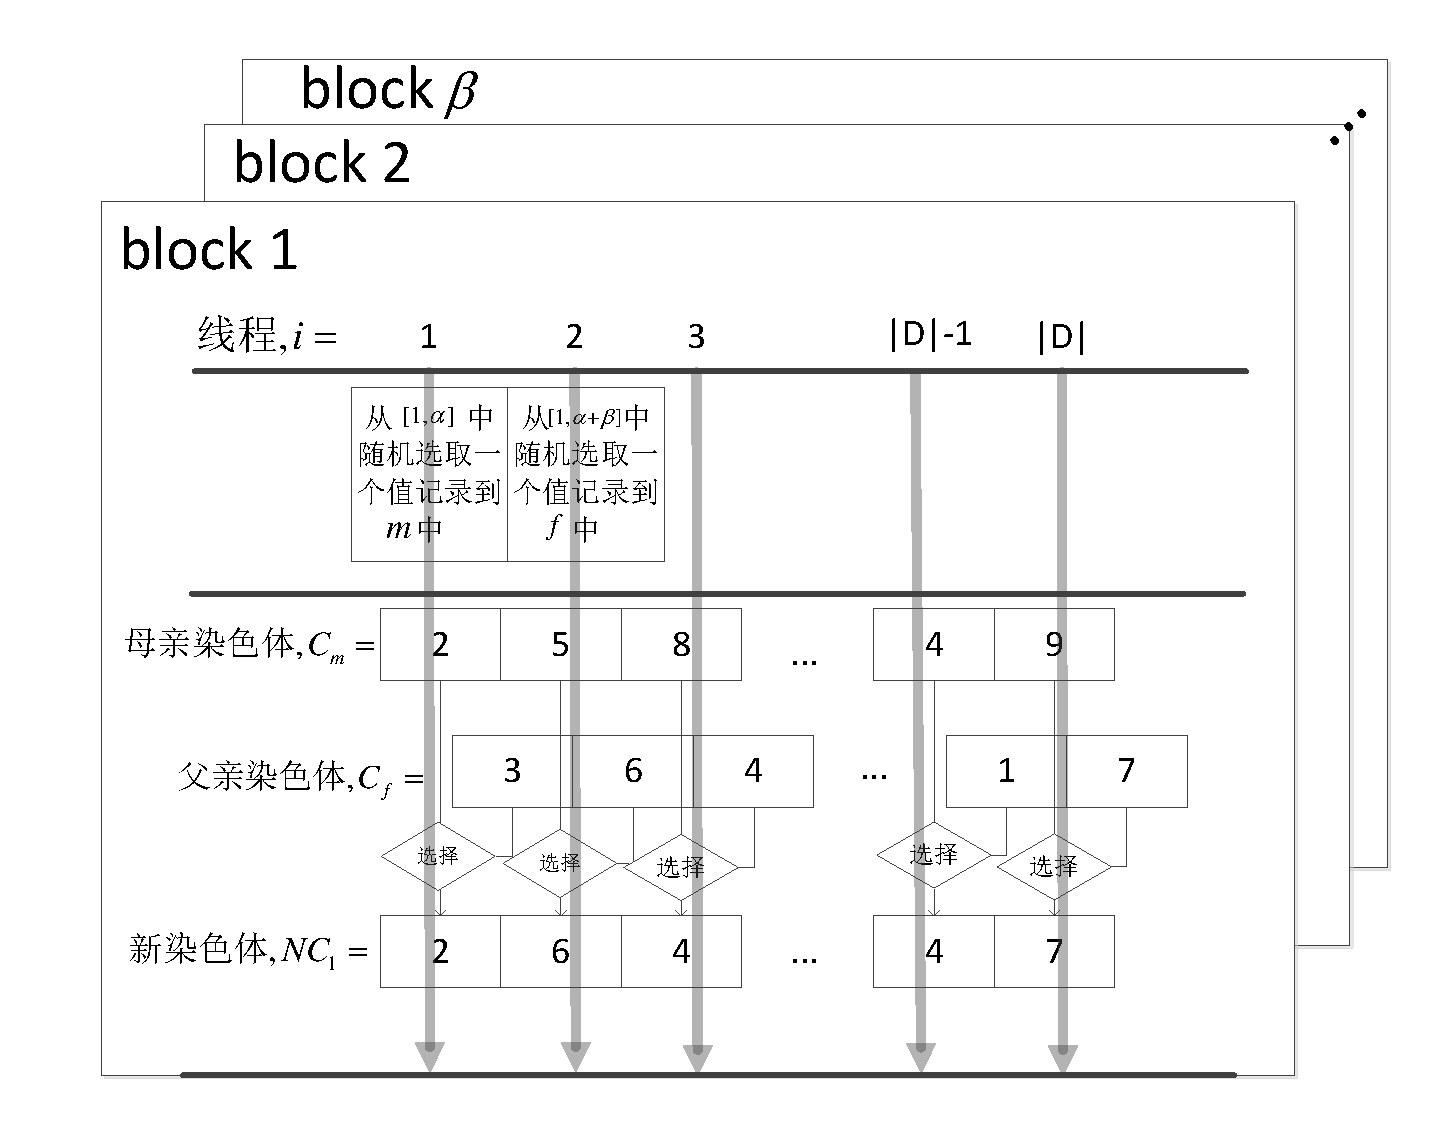
\includegraphics[width=0.8\textwidth]{figures/GPUcross.pdf}}
\end{center}
\caption{{\footnotesize{GPU并行均匀交叉过程}}}
\label{cross}
\end{figure}
\subsubsection{并行排序,变异与交叉}
在评价部分结束后,需要对所有的染色体按照代价函数的大小降序排序,本设计采用CUDA库Thrust\citing{Thrust}中提供的排序函数对GPU上的染色体进行排序,Thrust是基于标准模板库(STL)的CUDA C++模板库,Thrust为程序员提供常见的CUDA算法库,能够减少程序员工作量并且提高应用程序效率,Thrust库中的排序函数已经针对GPU架构做了很好得优化,所以本文不在对排序部分进行优化,排序函数细节可参考NVDIA官方文档\citing{Thrust}。

交叉过程只需要一个kernel,其并行示意图如图\ref{cross}所示,每个block负责一个新染色体的生成,通过之前的分析,一共需要生产$\beta$个新的染色体,所以GPU端一共需要分配$\beta$ 个block。每个block中的前两个线程需要先选择父母染色体,1号线程在$[1,\alpha]$中选择一个染色体作为母亲,2号线程在$[1,\alpha+\beta]$中选择一个染色体作为父亲。父母选取结束后,就可以进行均匀交叉了,其中每一个block中有|D|个线程来同时负责随机地从母亲染色体和父亲染色体的相应点位选择一个来作为新染色体相应点位的值,选择父亲或母亲的遗传基因的概率都是50\%,这样block内部的并行度达到$|D|$,总的并行粒度达到$\beta \cdot |D|$。

最后,对于变异部分,我们一共开辟$\gamma$个线程,每个线程随机在$A\cup B$集合中选取一个染色体,并随机选取$m$个点位进行变异,并行粒度为$\gamma$。

\section{基于拉格朗日的优化算法设计}

GA-PTEA算法虽然简单,但是其具有以下缺点:第一,需要事先计算大量备选路径,不能很好地适应网络的动态变化,一旦网络链路发生变化,又要重新计算备选路径。第二,遗传算法从开始到收敛需要大量的迭代次数,虽然经过GPU加速,但是由于收敛缓慢,仍然需要大量的计算时间。第三,遗传算法容易陷入局部最优解。

本节采用基于拉格朗日松弛的模型来解决业务量工程问题,并根据这个模型设计出并行算法LR-PTEA(Lagrange Relaxing Based Parallel Traffic Engineering Algorithm),LR-PTEA相对与GA-PTEA有以下优点:第一,LR-PTEA能够快速收敛。第二,LR-PTEA求得的解大大优于GA-PTEA。第三,LR-PTEA不需要事先产生备选路径,业务路由是实时计算出来的。
\subsection{基于拉格朗日松弛的模型}
在模型(\ref{Obj2},\ref{FlowConv},\ref{Capcon})中,网络容量约束(式子 \ref{Capcon}),把所有的路由变量联系到一起,因为这些变量的取值必修保证每一条链路上占用的流量小于链路的容量大小,正是由于存在链路容量约束,每个业务的路由选取才变得不相互独立,但是要利用GPU 的并行特性,需要寻找独立计算的可能性,因此,本文采用拉格朗日松弛方法,把一个业务量工程问题分解成一批业务的路由计算问题,而这些业务的路由计算问题是相互独立的,很适合并行计算。

将模型(式子\ref{Obj2},\ref{FlowConv},\ref{Capcon})中的网络容量约束松弛进目标函数得到如下拉格朗日子问题:
\begin{equation}\label{LagProb}
\begin{split}
L(\mathbf{\lambda})= min\sum\limits_{d \in D}\sum\limits_{(i,j) \in E_b} w_{ij}\cdot x_{ij}^d\cdot bw_d+ \\ ~~~~~\sum\limits_{(i,j) \in E_b}\lambda_{ij}(\sum\limits_{d \in D} x_{ij}^d \cdot bw_d-c_{ij})
\end{split}
\end{equation}
其中 $\lambda_{ij}$ 表示链路 $(i,j)$的拉格朗日乘子。

表达式(\ref{LagProb})还可以表示为:
\begin{equation}\label{Lagprob1}
L(\mathbf{\lambda})= min\sum\limits_{d \in D}\sum\limits_{(i,j) \in E_b} (w_{ij}+\lambda_{ij})x_{ij}^d \cdot bw_d -\sum\limits_{(i,j) \in E_b}\lambda_{ij}c_{ij}
\end{equation}
受限于:
\begin{equation}\label{FlowConv2}
\begin{split}
\sum\limits_{(i,j) \in E_b} x_{ij}^d - \sum\limits_{(j,i) \in E_b} x_{ji}^d
=\begin{cases}
1 & \text{if $i = s_d$}\\
-1 & \text{if $i = t_d$} \\
0 &{otherwise}
\end{cases}
\\~~~~~~~~\forall i\in V_b, \forall d\in D
\end{split}
\end{equation}
拉格朗日子问题的目标函数中的$\sum_{(i,j) \in E_a}\lambda_{ij}c_{ij}$这一项,不随着拉格朗日乘子的变化而变化,本文将其作为常数项而丢掉不讨论,丢掉$\sum_{(i,j) \in E_a}\lambda_{ij}c_{ij}$ 这一项后,拉格朗日子问题的目标函数中只含有代价部分 $w_{ij}+\lambda_{ij}$和$x_{ij}^d\cdot bw_d$的乘积。注意到$\sum_{(i,j) \in E_a} (w_{ij}+\lambda_{ij})x_{ij}^d\cdot bw_d$表示业务$d$的路由代价,因此,拉格朗日子问题的目标函数是最小化所有业务的路由代价之和,观察这个子问题的约束,我们发现,每一个约束都只含有一个和业务需求相关的变量,所以,这个拉格朗日子问题可以被分解成一系列独立的最短路径问题(每个业务需求对应于一个最短路问题),只是这些最短路径问题的链路代价发生了改变,链路代价变得和拉格朗日乘子 $\mathbf{\lambda}$ 相关。也就是说给定一个拉格朗日乘子$\mathbf{\lambda}$,我们可以将拉格朗日子问题看成一批单业务的最短路径问题,我们可以通过并行地计算一系列的最短路径来解决这个拉格朗日子问题。

因为把容量约束松弛进代价函数中后,不会增加目标函数的值, $L(\mathbf{\lambda})$成为原问题最优目标函数值的下界,$z^* \ge L(\mathbf{\lambda})$,为了得到最紧的的下界值,我们要解决以下这个优化问题:
\begin{equation}\label{dual}
L^*(\mathbf{\lambda^*}) = maximize_{\mathbf{\lambda}}L(\mathbf{\lambda})
\end{equation}
~~受限于: (\ref{FlowConv2})
\vskip 0.2cm

以上的这个优化问题也被称为原来业务量工程问题(式子\ref{Obj2},\ref{FlowConv},\ref{Capcon})的对偶问题 \citing{NetworkFlow},其中$\mathbf{\lambda^*}$ 表示最优拉格朗日乘子,为了得到最优乘子$\mathbf{\lambda^*}$,可以使用次梯度优化算法来解决,次梯度优化计算时,第一次先初始化乘子 $\mathbf{\lambda}^0$,然后通过式子\ref{iter}来更新乘子:
\begin{equation}\label{iter}
\mathbf{\lambda}_{ij}^{(k+1)} =\mathbf{\lambda_{ij}}^{(k)}+\theta_{k} g^{(k)}= \mathbf{\lambda_{ij}}^{(k)} + \theta_k[(\sum\limits_{d \in D}x_{ij}^d\cdot bw_d- c_{ij})]^+
\end{equation}
其中, $\mathbf{\lambda}_{ij}^{(k)}$表示第$k$次迭代的对应于边$(i,j)$的拉格朗日乘子, $g^{(k)}$是$L(\mathbf{\lambda})$ 对$\mathbf{\lambda}^{k}$的任意一种次梯度,$\theta_k$ 表示第$k$次的迭代的步长,标记$[\alpha]^+$ 表示$\alpha$中符号为正的部分,也就说$[\alpha]^+=max(\alpha, 0)$,从表达式\ref{iter}可以看出来如果链路$(i,j)$ 上的流量总和超过链路$(i,j)$上的容量,链路$(i,j)$ 上的$\lambda_{ij}^k$拉格朗日乘子会增加,也就是表示一些业务流量需要从链路$(i,j)$上移除,另外,为了避免产生负权重的链路代价,当链路容量大于其上的流量时,我们并不去减小此链路$(i,j)$上的$\lambda_{ij}^k$。

根据以上讨论,我们给出基于拉格朗日乘子法的并行业务量工程算法的框架,如图\ref{lpl}所示,LR-PTEA主要包括以下步骤:

步骤一,为$G(V, E)$初始化链路权重。

步骤二,计算所有业务的最短路径,其中路径计算任务被分配到GPU上进行并行计算。

步骤三,为了从当前计算出来的路径中得到原问题的优化目标函数值,对步骤二中计算出来的路径进行调整。

步骤四,更新链路权重,更新完毕后,如果停止条件不满足,则回到步骤二,进入下一轮迭代。
\begin{figure}
\vspace{-1cm}
\setlength{\abovecaptionskip}{-0.5cm}
\begin{center}
{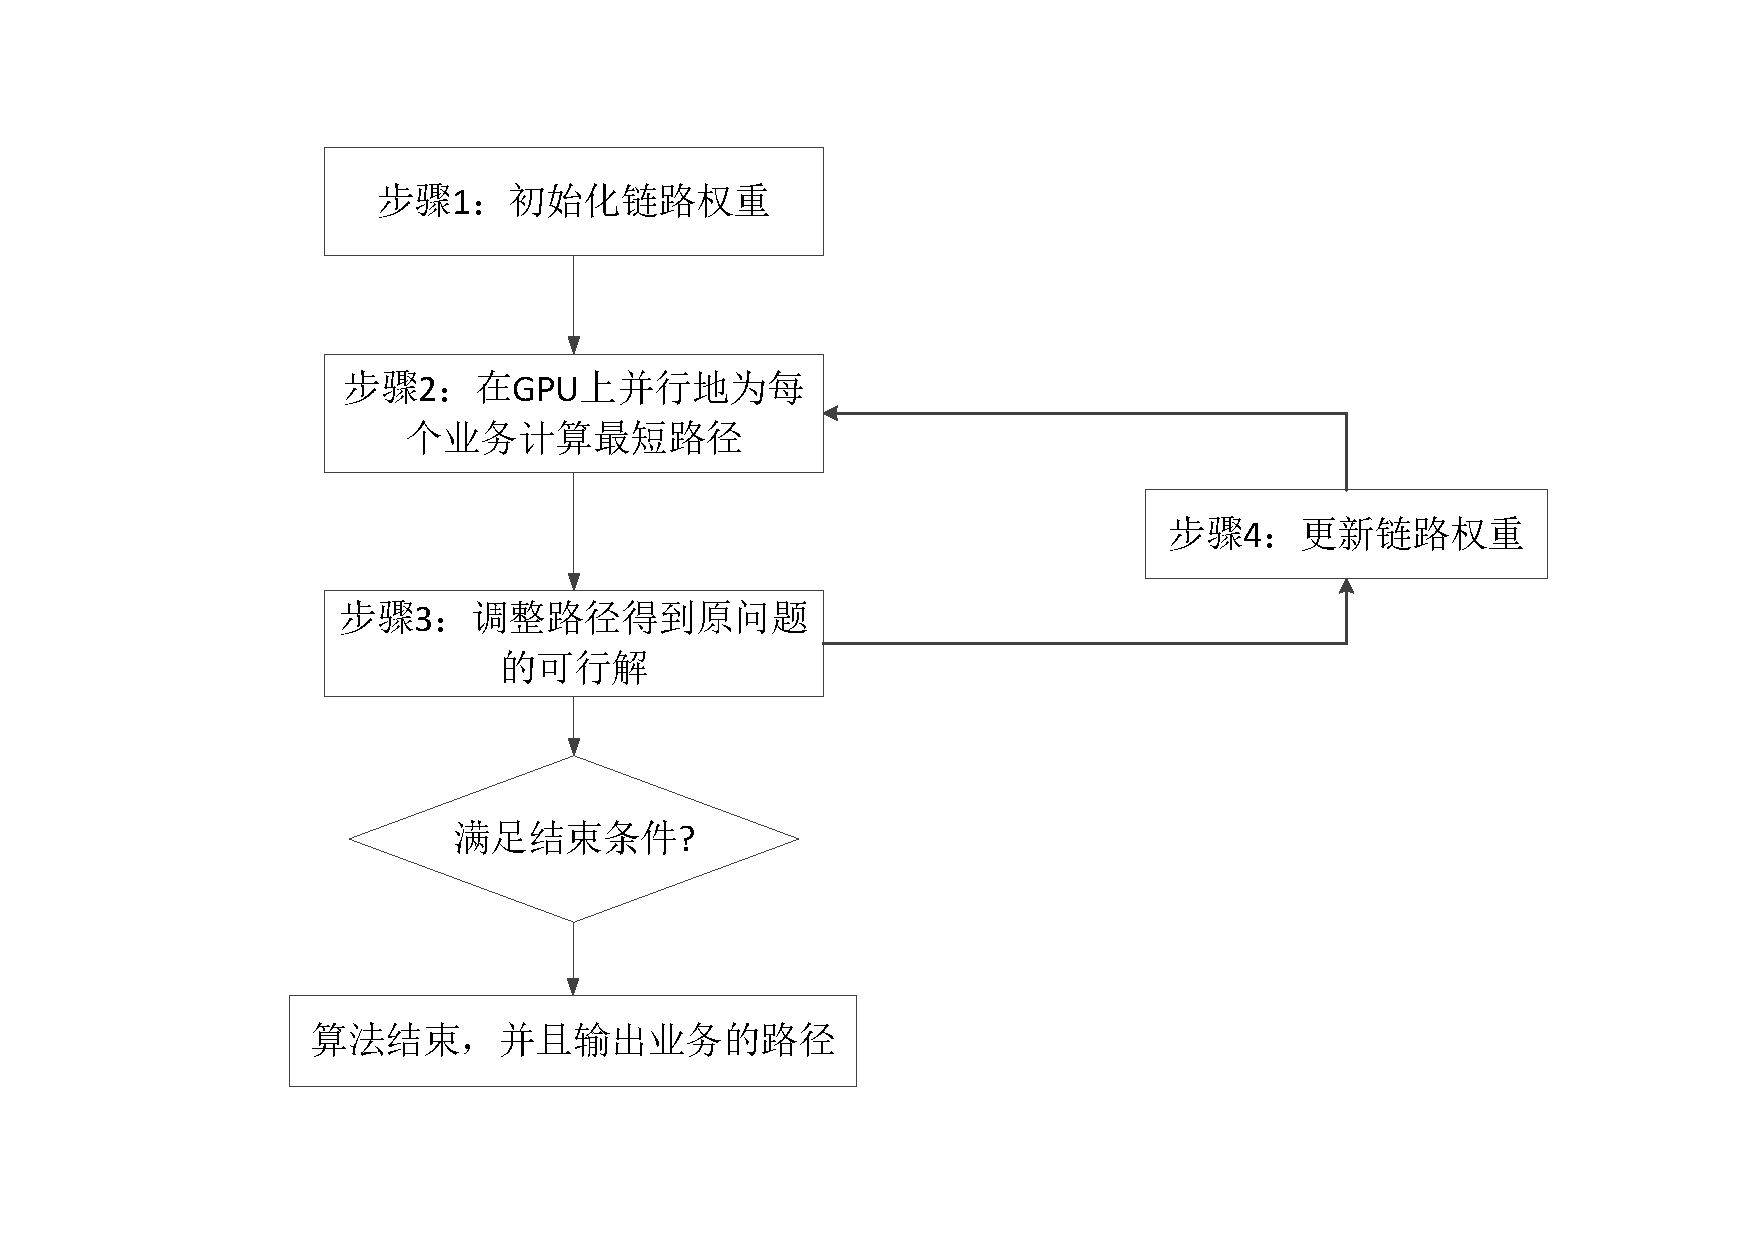
\includegraphics[width=1\textwidth]{figures/lagrange.pdf}}
\end{center}
\caption{{\footnotesize{LR-PTEA算法流程图}}}
\label{lpl}
\end{figure}
\subsection{基于GPU的并行路由计算}
在每次迭代中,LR-PTEA为每个业务 $d \in D$在图 $G(V, E)$中计算最短路径,显然,丢掉链路容量约束后,不同业务的最短路径计算可以独立地在GPU上并行执行,但是,最短路算法的逻辑对于GPU来说太过复杂,GPU最初是被设计来做大规模的数值计算问题,其只实用于逻辑比较简单,但是数值计算量较大的任务,所以在GPU上直接开辟一个线程来计算一个业务的路径,不仅仅在计算上是低效的,而且这样的并行粒度也不能充分利用GPU 的大规模并行能力。为了提高并行粒度,LR-PTEA对最短路径算法也进行并行化设计。

文章 \citing{SSP1}提出一种Dijkstra最短路径算法在GPU上的并行实现,但是从算法结构上分析,Dijkstra最短路径算法并不适应于并行算法的设计,所以Dijkstra最短路径算法在GPU上的实现不能得到很好的加速效果。为了得到更好的加速效果,LR-PTEA选择Bellman-Ford \citing{NetworkFlow}最短路算法来进行并行实现。Bellman-Ford最短路算法逐步地减小距离标记 $Dist[v]$($v\in V$),直到其收敛到真实的最短距离。串行的Bellman-Ford算法流程如算法\ref{Bellman}所示,其中 $Dist[v]$ 表示距离起点$s$到$v$的最短路径距离,$Pre[v]$ 表示点$s$到点$v$ 的最短路径上$v$ 的前驱节点,在初始化好了所有节点的距离数组和前驱节点数组之后,Bellman-Ford算法最多迭代 $|V|$ 次,每一次迭代,算法都会松弛图$G(V, E)$中的所有的边(第10-11行)。Bellman-Ford 算法的算法复杂度为$(|V|\cdot |E|)$,他的复杂度一般是高于Dijkstra最短路径算法的复杂度,但是,因为Bellman-Ford算法每次松弛边的操作都是独立无关的,Bellman-For算法很容易在GPU上实现并行化。

图 \ref{ParFramework} 中显示了LR-PTEA的最短路径计算的并行实现框架。首先,根据业务的源节点将业务分配成不同的组,使得每一组内业务的源节点相同。我们假设第$i$个组的源节点为$s_i$。 然后,每一组的最短路径计算使用$m$个GPU 线程的并行地进行边的松弛操作,如图\ref{ParFramework}所示,线程$T_{i,j}$负责为对应于源点$s_i$的链路$e_{j}$ 进行松弛操作。因此总的并行执行的线程数是$m \times n$,其中$m$和$n$分别表示链路数目和业务组的数目。

在本文的最短路算法的并行实现中,每个block内部的线程都松弛同一条链路,比如,在图 \ref{GB} 中,集合$\{T_{1j}, T_{2j}, \cdots, T_{ij}, \cdots, T_{nj}\}$都在$block_j$上执行,其中 $T_{ij}$为对应源节点为$s_i$ 的链路$e_i$执行松弛操作,其中,我们设链路$e_i$的头节点和尾节点分别为$h_i$ 和$t_i$。可以看到,当存在链路更新时,标记$Mark$会被设置成1,这是为了优化算法的迭代次数,当某次迭代结束$Mark=0$ 则表示这次迭代没有边进行了更新操作,说明Bellman 算法已经提前结束,我们的实验证明这一个优化可以大大地减小Bellman算法的迭代次数。
\begin{algorithm}[htb]
\begin{algorithmic}[1]
\Require
网络拓扑:$G(V, E)$;
源点:$s$;
\Ensure
从$s$开始到其他点的路径集合$P$;
\For {$v \in V$}
\State {$Dist[v] \leftarrow \infty$}
\State {$Pre[v] \leftarrow $ NIL}
\EndFor
\State {$Dist[s] \leftarrow 0$}
\State {$Mark \leftarrow 1$}
\While {$Mark > 0$}
\State {$Mark \leftarrow 0$}
\For{$(u,v) \in E$}
\If{$Dist[v]>Dist[u]+w_{uv}$}
\State {$Dist[v] \leftarrow Dist[u]+w_{uv}$}
\State {$Pre[v] \leftarrow u$}
\State {$Mark = 1$}
\EndIf
\EndFor
\EndWhile
\State {根据前驱数组$Pre$,重新构建最短路集合,输出路径到集合$P$}
\end{algorithmic}
\caption{{Bellman-Ford最短路算法}}
\label{Bellman}
\end{algorithm}


\begin{figure*}
\vspace{-0.5cm}
\setlength{\abovecaptionskip}{-0.5cm}
\begin{center}
{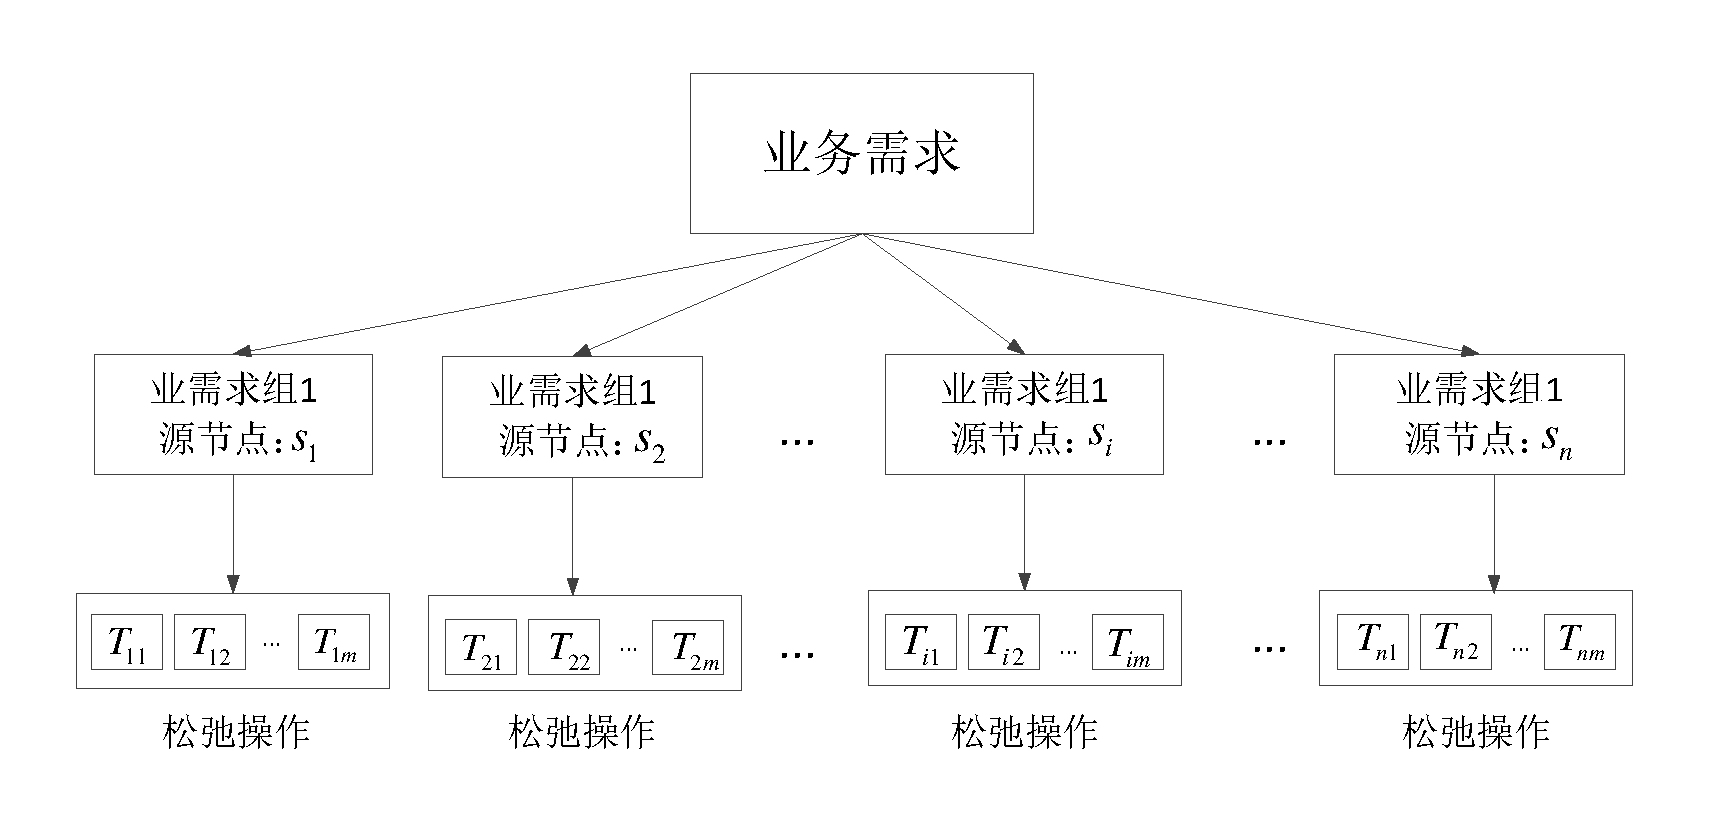
\includegraphics[width=1 \textwidth]{figures/paframework.pdf}}
\end{center}
\caption{{\footnotesize{并行业务计算框架}}}
\label{ParFramework}
\end{figure*}




\begin{figure*}
\vspace{-0.4cm}
\setlength{\abovecaptionskip}{-0.5cm}
\begin{center}
{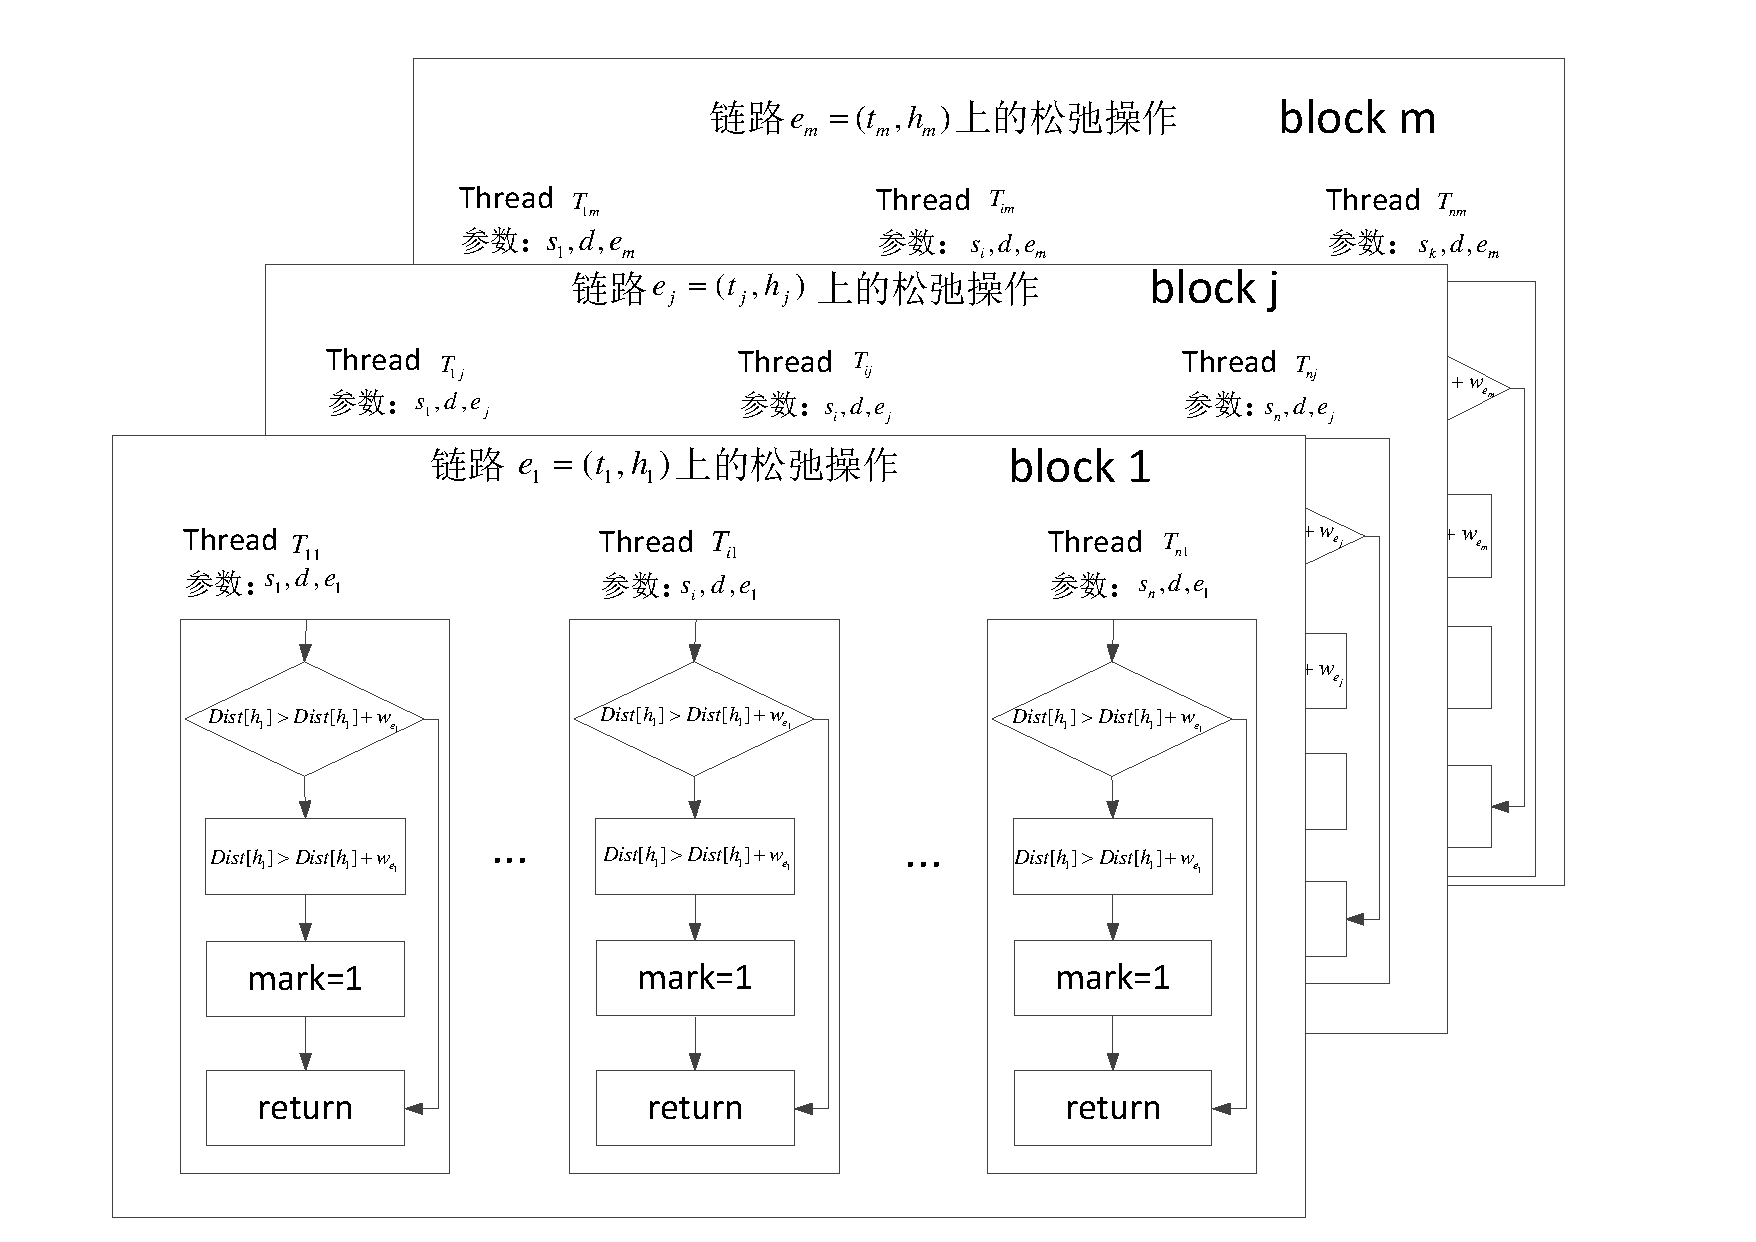
\includegraphics[width=1 \textwidth]{figures/GPUimpl.pdf}}
\end{center}
\caption{{\footnotesize{GPU上Bellman算法的实现}}}
\label{GB}
\end{figure*}

\begin{figure*}
\setlength{\abovecaptionskip}{-0.5cm}
\begin{center}
{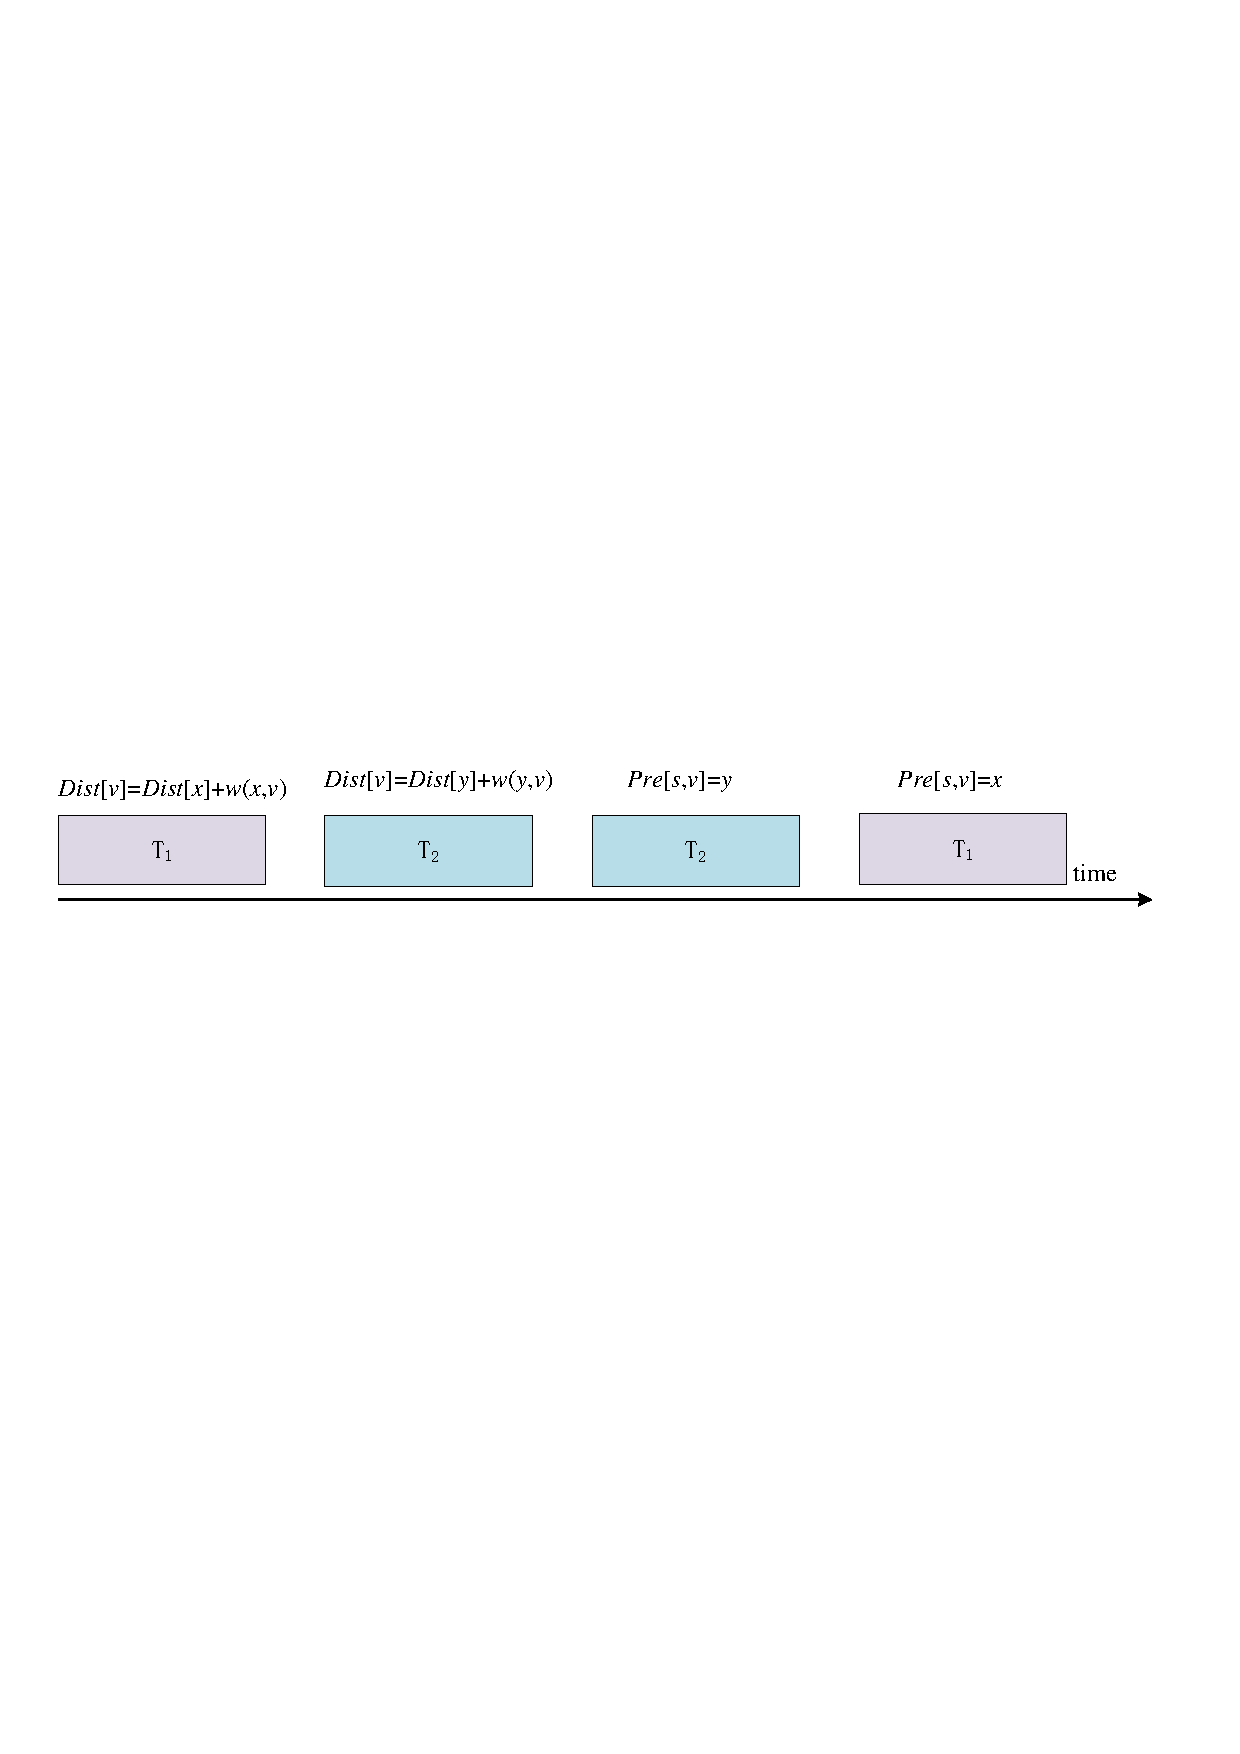
\includegraphics[width=0.8 \textwidth]{figures/SynPro.pdf}}
\end{center}
\caption{{\footnotesize{同步问题的例子}}}
\label{SynPro}
\end{figure*}
多业务的并行Bellman算法的CUDA实现如算法\ref{kd}所示。需要注意的是由于线程在GPU上是独立执行的,在更新节点的距离标记和前驱标记的时候会出现同步问题,假设线程$T_1$为链路$(x,v)$执行松弛操作,而线程$T_2$为链路$(y,v)$ 执行松弛操作,假设两个线程更新点$v$ 的距离标记和更新前驱标记的顺序如图\ref{SynPro} 所示,如果$Dist[y] + w(y, v) < Dist[x] +w(x, v)$,那么$Dist[v]$ 被更新为$Dist[y] + w(y, v)$,但是由于更新的顺序发生交叉,节点$v$的前驱节点被更新成了$x$, 而不是真正正确的前驱节点$y$。为了避免这个同步问题,我们使用两个kernel,一个kernel\_distance\_update(算法\ref{KernelDist})用来更新距离标号,一个kernel\_predecessor\_update(算法\ref{KernelPre})用来更新前驱节点。

如算法\ref{KernelDist}所示,在kernel\_distance\_update中,线程先寻址到其对应的边$e$和其对应的源节点标号$s$,然后对边进行松弛操作,其中$e.head$表示有向边$e$的目的节点,$e.tail$表示有向边$e$的出发节点。如算法\ref{KernelPre}所示,在kernel\_predecessor\_update中,线程判断$Dist[s][e.tail] + e.weight$是否等于$Dist[s][e.head]$,因为这时$Dist$数组已经是最短距离数组了,如果条件成立,那么$e.tail$就有资格作为$e.head$的最优前驱节点,算法就对前驱数组$Pre$进行更新。

\begin{algorithm}[t]
\begin{algorithmic}[1]
\Require
业务需求集合$D$;
链路集合$E$;
\Ensure {业务需求的最短路径集合$P$}
\State {将业务的源节点加入到集合$S$中}
\State {$Mark \leftarrow$ 1}
\While{$Mark > 0$}
\State {$Mark \leftarrow$ 0}
\State {发射 kernel\_distance\_update($S$, $E$, $Dist$)}
\EndWhile
\State {发射 kernel\_predecessor\_update($S$, $E$, $Dist$, $Pre$)}
\State {根据前驱数组$Pre$重建业务的最短路径,并把路径加入到集合$P$中}
\end{algorithmic}
\caption{{并行最短路计算过程}}
\label{kd}
\end{algorithm}

\begin{algorithm}[t]
\begin{algorithmic}[1]
\Function{kernel\_distance\_update}{$S$, $E$, $Dist$}
\State {$bid \leftarrow$ block ID}
\State {$tid \leftarrow$ thread ID}
\State {$s \leftarrow S[tid]$}
\State {$e \leftarrow E[bid]$}
\If{$Dist[s][e.tail] + e.weight < Dist[s][e.head]$}
\State {$Mark \leftarrow 1$}
\State {$Dist[s][e.head] \leftarrow Dist[s][e.tail] + e.weight$}
\EndIf
\EndFunction
\end{algorithmic}
\caption{kernel 函数kernel\_distance\_update}
\label{KernelDist}
\end{algorithm}

\begin{algorithm}[t]
\begin{algorithmic}[1]
\Function {kernel\_predecessor\_update}{$S$, $E$, $Dist$,$Pre$}
\State {$bid \leftarrow$ block ID}
\State {$tid \leftarrow$ thread ID}
\State {$s \leftarrow S[tid]$}
\State {$e \leftarrow E[bid]$}
\If{$Dist[s][e.tail] + e.weight = Dist[s][e.head]$}
\State {$Pre[s][e.head]= e.tail$}
\EndIf
\EndFunction
\end{algorithmic}
\caption{kernel函数 kernel\_predecessor\_update}
\label{KernelPre}
\end{algorithm}
\subsection{链路权重更新}
\subsubsection{权重更新步长}
在LR-PTEA算法中,在第$k+1$次迭代,链路$(i,j)$的权重被更新为$w_{ij}^{k} + \lambda_{ij}^{k+1}$, 其中$\lambda_{ij}^{k+1}$ 被更新为:
\begin{equation}\label{Iter}
\lambda_{ij}^{k+1} = \lambda_{ij}^k + \theta_k[(\sum\limits_{d \in D}x_{ij}^d \cdot bw_d - c_{ij})]^+.
\end{equation}
为了保证收敛性,第$k$次迭代的更新步长$\theta_k$可以被设置为 $\frac{1}{k}$ \citing{NetworkFlow}。 然而,通过仿真发现,当$\theta_k$被设置为 $\frac{1}{k}$时,其收敛缓慢。让我们考虑图 \ref{u1}的例子,其中链路$(i,j)$ 上的标记分别表示链路权重和链路上剩余的容量大小。假设现在有两个业务需求$d_1$ 和$d_2$,他们的源都是$A$,目的节点都是$D$,且每一个业务的流量大小都是4个单位。为了展示这个迭代过程,我们把算法前5次的迭代结果表示在表 \ref{Iterprocess1}中,从表中可以看到,业务计算出的最短路径一直在$A-B-D$和$A-C-D$ 之间徘徊。算法必修等到$A-B-D$ 和$A-C-D$ 的两条路的权重相等时才能停止,只有这样这两个业务才可能分离,其中一个选择$A-B-D$,而另一个选择$A-C-D$。 但是,正如表中所示这需要大量的迭代才能达到。
\begin{figure}
\setlength{\abovecaptionskip}{-0.5cm}
\begin{center}
{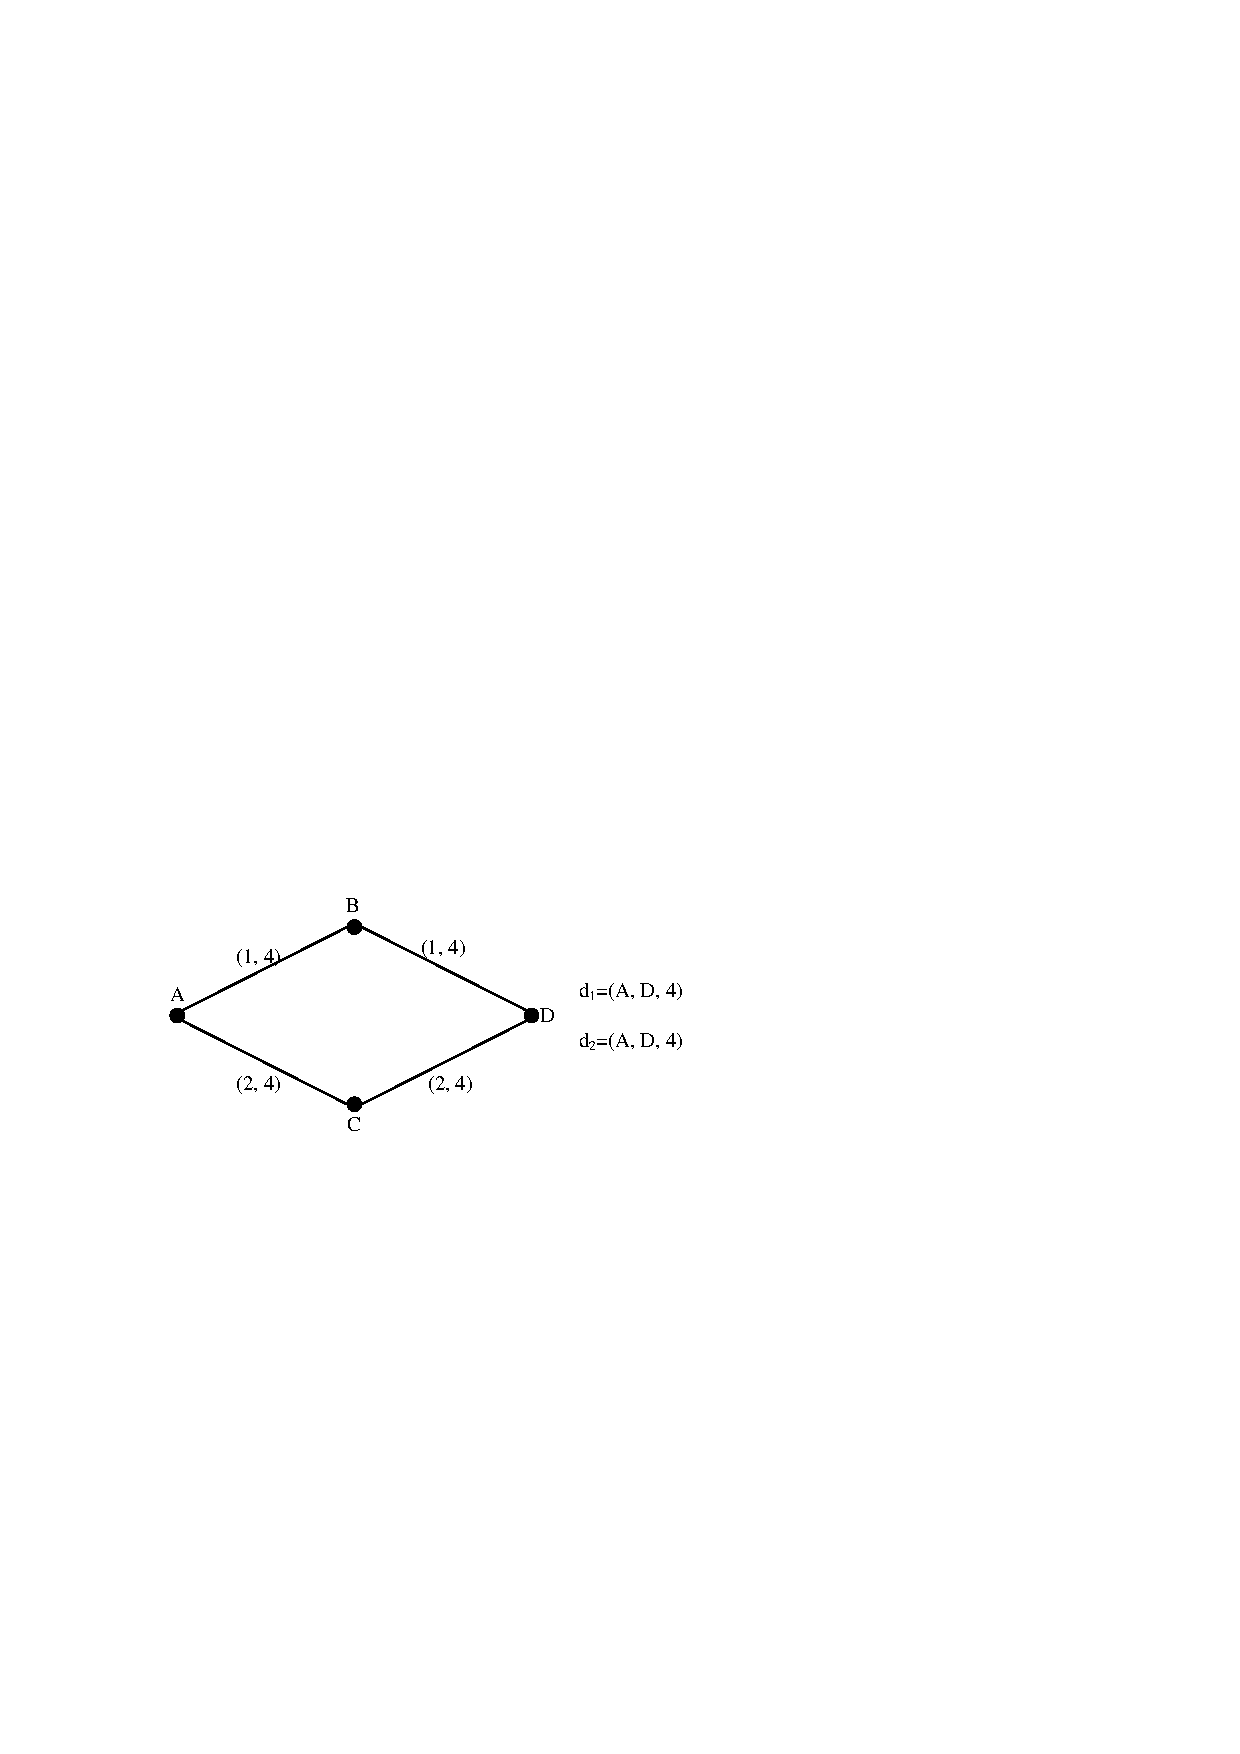
\includegraphics[width=0.4 \textwidth]{figures/IterNum.pdf}}
\end{center}
\caption{{\footnotesize{链路更新例子(1)}}}
\label{u1}
\end{figure}
\begin{table}[t]
\newcommand{\tabincell}[2]{\begin{tabular}{@{}#1@{}}#2\end{tabular}}
\setlength{\abovecaptionskip}{0.2cm}
\centering
\scriptsize{
\renewcommand{\tabcolsep}{0.09cm}
\renewcommand{\arraystretch}{1.2}
\caption{拉格朗日更新过程(1)}
\begin{tabular}{| c | c | c | c|}
\hline
Iteration number & \tabincell{l}{Calculated paths for \\the two demands} & Path weights & $\theta_k$
\\ \hline
0 & \tabincell{l}{A-B-D \\ A-B-D} & \tabincell{l}{2(1+1) \\ 2(1+1)} & 1 \\ \hline
1 & \tabincell{l}{A-C-D \\ A-C-D } & \tabincell{l}{4(2+2) \\ 4(2+2)} & 1 \\ \hline
2 & \tabincell{l}{A-B-D \\ A-B-D} & \tabincell{l}{10(1+4+1+4) \\ 10(1+4+1+4)} & 0.5 \\ \hline
3 & \tabincell{l}{A-C-D\\ A-C-D} & \tabincell{l}{12(2+4+2+4) \\ 12(2+4+2+4)} & 0.33 \\ \hline
4 & \tabincell{l}{A-B-D \\ A-B-D} & \tabincell{l}{14(1+6+1+6) \\ 14(1+6+1+6)} & 0.25 \\ \hline
5 & \tabincell{l}{A-C-D \\ A-C-D} & \tabincell{l}{14.66(2+5.33+2+5.33) \\ 14.66(2+5.33+2+5.33)} & 0.2 \\ \hline
\end{tabular}
\vskip 0.2 cm
\label{Iterprocess1}
}
\end{table}

另外一种常用的步长选择是:
\begin{equation}\label{StepSize}
\theta_k = \frac{\rho[UB-{L(\mathbf{\lambda}^k)]}}{||\mathbf{Ax^k}-\mathbf{b}||^2}
\end{equation}
其中$UB$是最优化目标函数的上界,$\rho$是一个取值范围为0到2的常数,$\mathbf{A}$ 和 $\mathbf{b}$分别是链路相关矩阵和链路上的剩余容量向量。但是从实验中发现设置这种步长迭代效果也不令人满意。

本设计采用一种简单但是有效的链路权重更新步长,假设$\theta_{k}^{ij}$ 为第$k$次迭代时链路$(i,j)$ 上的需更新的步长,那么$\theta_{k}^{ij}$ 为:
\begin{equation}\label{StepSizeUsed}
\theta_{k}^{ij} = \frac{1}{|c_{ij}-\sum\limits_{d \in D} x_{ij}^d bw_d|}
\end{equation}

从式子 \ref{StepSizeUsed},我们可以看到,如果一条链路上承载的流量大小超过了这条链路上的容量大小,那么这条链路上的权重在下一次迭代之前就会增加1,对于其他的流量满足约束的链路,其权重不会改变,如果使用式子\ref{StepSizeUsed}的步长更新方法,LR-PTEA仅仅只需要一次迭代就能够得到例子(图\ref{u1})中的最优的权重。我们的实验表明,这种粗粒度的更新操作大大的减小了算法的收敛迭代次数,从而大大缩短算法运行时间。
\subsubsection{随机更新策略}

拉格朗日松弛法将原问题分解成了一个个独立的最短路径问题,这样使得算法可以进行并行化设计。但是由于每个子问题独立分离,使得每个问题在求最短路径时都是贪心的,这样可能会使得大量业务抢占同一批链路,造成拥塞,一旦拥塞,链路的权重就会增加,又会使得大量的业务集体放弃这一批链路,去抢占其他链路,使得其他链路也发生拥塞,形成一种恶性循环,最终会使得算法提前收敛到局部最优解。另外,为了追求快速收敛,我们简单地把每一个超过容量约束的边增加1,这样粗粒度的增加,可能会加重上面讨论的拥塞循环。
\begin{figure}
\setlength{\abovecaptionskip}{-0.5cm}
\begin{center}
{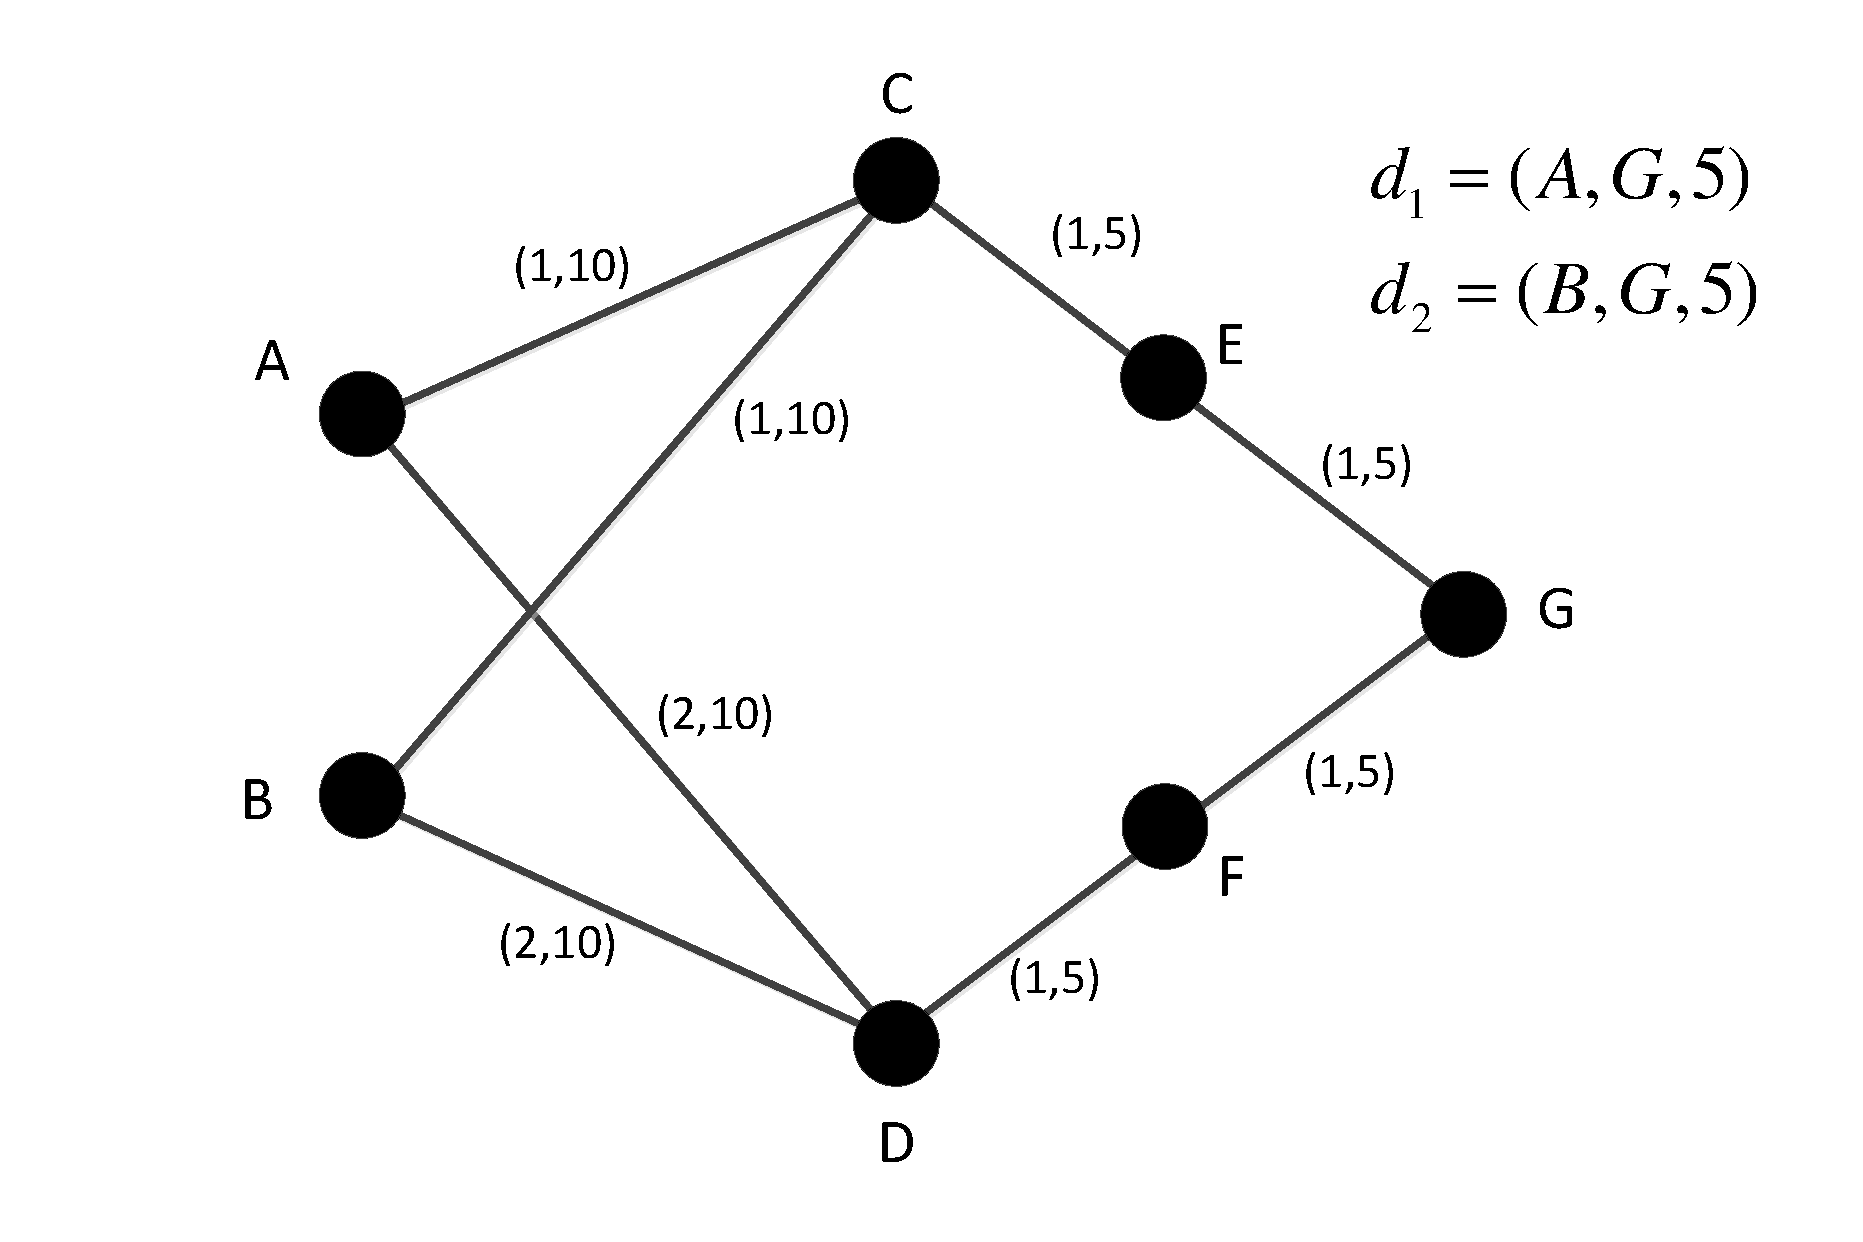
\includegraphics[width=0.4 \textwidth]{figures/random.pdf}}
\end{center}
\caption{{\footnotesize{链路更新例子(2)}}}
\label{u2}
\end{figure}

如图\ref{u2}所示,假设存在两个业务$d_1$和$d_2$,其中$d_1$的源节点为$A$,目的节点为$G$,其流量大小为$5$,$d_2$ 的源节点为$B$,目的节点为$G$,其流量大小也为$5$。开始时两个都分别贪心地计算最短路径,$d_1$选择路径$A-C-E-G$,$d_2$选择路径$B-C-E-G$,这样的话,链路$C-E$和$E-G$出现拥塞,表 \ref{Iterprocess2} 展示了这个迭代过程。图 \ref{u2}中最优的选择是让其中一个业务经过边$C-E-G$进行中继,另一个业务经过边$D-F-G$进行中继。但是迭代过程始终无法使得两条链路发生分离,图中的链路权重始终无法达到最优条件,这是因为链路$C-E-G$和链路$D-F-G$每次超限都会为路径的总权重增加2个单位,权重增加的粒度太大。假设每次迭代时链路$C-E-G$总共只增加一个单位,那么算法只需要一次迭代就能达到最优条件,此时链路$C-E-G$由于超限,权重一共增加1个单位,那么路径$A-C-E-G$ 和路径$A-D-F-G$ 权重相等都为4,同样,路径$B-C-E-G$和路径$B-D-F-G$的权重也相等了,这样两个业务才会分离开(比如业务$d_1$选择链路$A-C-E-G$,业务$d_2$选择链路$B-D-F-G$)。为了解决链路增加粒度过大的情况,在本设计中我们采用随机更新的策略,也就是对一条流量超过容量约束的边$(i,j)$,我们以概率$\phi$ 来对他进行权重更新,每条边的权重增加粒度依然为1个单位,假设$\phi=0.5$,这种方法在一定概率上保证图 \ref{u2} 中的例子可以在一次迭代中收敛。我们的实验发现这种更新策略能够在保证算法收敛速度的同时,求解到更加优化的解。
\begin{table}[t]
\newcommand{\tabincell}[2]{\begin{tabular}{@{}#1@{}}#2\end{tabular}}
\centering
\scriptsize{
\renewcommand{\tabcolsep}{0.09cm}
\renewcommand{\arraystretch}{1.2}
\caption{拉格朗日更新过程(2)}
\begin{tabular}{| c | c | c |}
\hline
Iteration number & \tabincell{l}{Calculated paths for \\the two demands} & Path weights
\\ \hline
0 & \tabincell{l}{A-C-E-G \\ B-C-E-G} & \tabincell{l}{3(1+1+1) \\ 3(1+1+1)} \\ \hline
1 & \tabincell{l}{A-D-F-G \\ B-D-F-G } & \tabincell{l}{4(2+1+1) \\ 4(2+1+1)} \\ \hline
2 & \tabincell{l}{A-C-E-G \\ B-C-E-G} & \tabincell{l}{5(1+2+2) \\ 5(1+2+2)} \\ \hline
3 & \tabincell{l}{A-D-F-G\\ B-D-F-G} & \tabincell{l}{6(2+2+2) \\ 6(2+2+2)} \\ \hline
4 & \tabincell{l}{A-C-E-G \\ B-C-E-G} & \tabincell{l}{7(1+3+3) \\ 7(1+3+3)} \\ \hline
5 & \tabincell{l}{ ...\\ ...} & \tabincell{l}{... \\ ...}\\ \hline
\end{tabular}
\vskip 0.2 cm
\label{Iterprocess2}
}
\end{table}
\subsection{路径调整}
注意到,在最优的权重代价(最优拉格朗日乘子)下,LR-PTEA求解到的路径集合解是拉格朗日对偶问题的优化解,但是它不一定是原来业务量工程问题的可行解。作为一个例子,考察图 \ref{ppt}中的情况,图中的元组中数字分别表示链路的代价和链路上的剩余容量大小。我们假设有两个业务需求$d_1$和$d_2$,其中两个业务的流量需求都是1个单位,假设在某一个迭代过程中,LR-PTEA为两个业务算出来的链路分别为$A-C-E-D$和$B-C-E-F$,这种路径选择是对偶问题的最优解,但是他不是原问题的可行解,因为链路$(C,E)$ 上承载的链路容量大于了链路$(C,E)$ 上的容量。这是由于每个业务在选择路径的时候没有去考虑其他业务所选择的路径,但是我们容易看到这个例子中所有路径权重都一样(都等于3),也就是说,图中存在着大量的等价链路,但是在这个例子中两个业务恰好都选择了冲突的那一条路径$A-C-E-D$,如果业务$d_1$的路径被调整到$A-D$,业务$d_2$的链路被调整到$B-F$,那么,我们可以得到原问题的最优可行解。所以通过这里的启发,我们发现需要设计一种业务路径调整算法来主动避免链路出现冲突,以得到原问题的可行解。
\begin{figure}
\setlength{\abovecaptionskip}{-0.5cm}
\begin{center}
{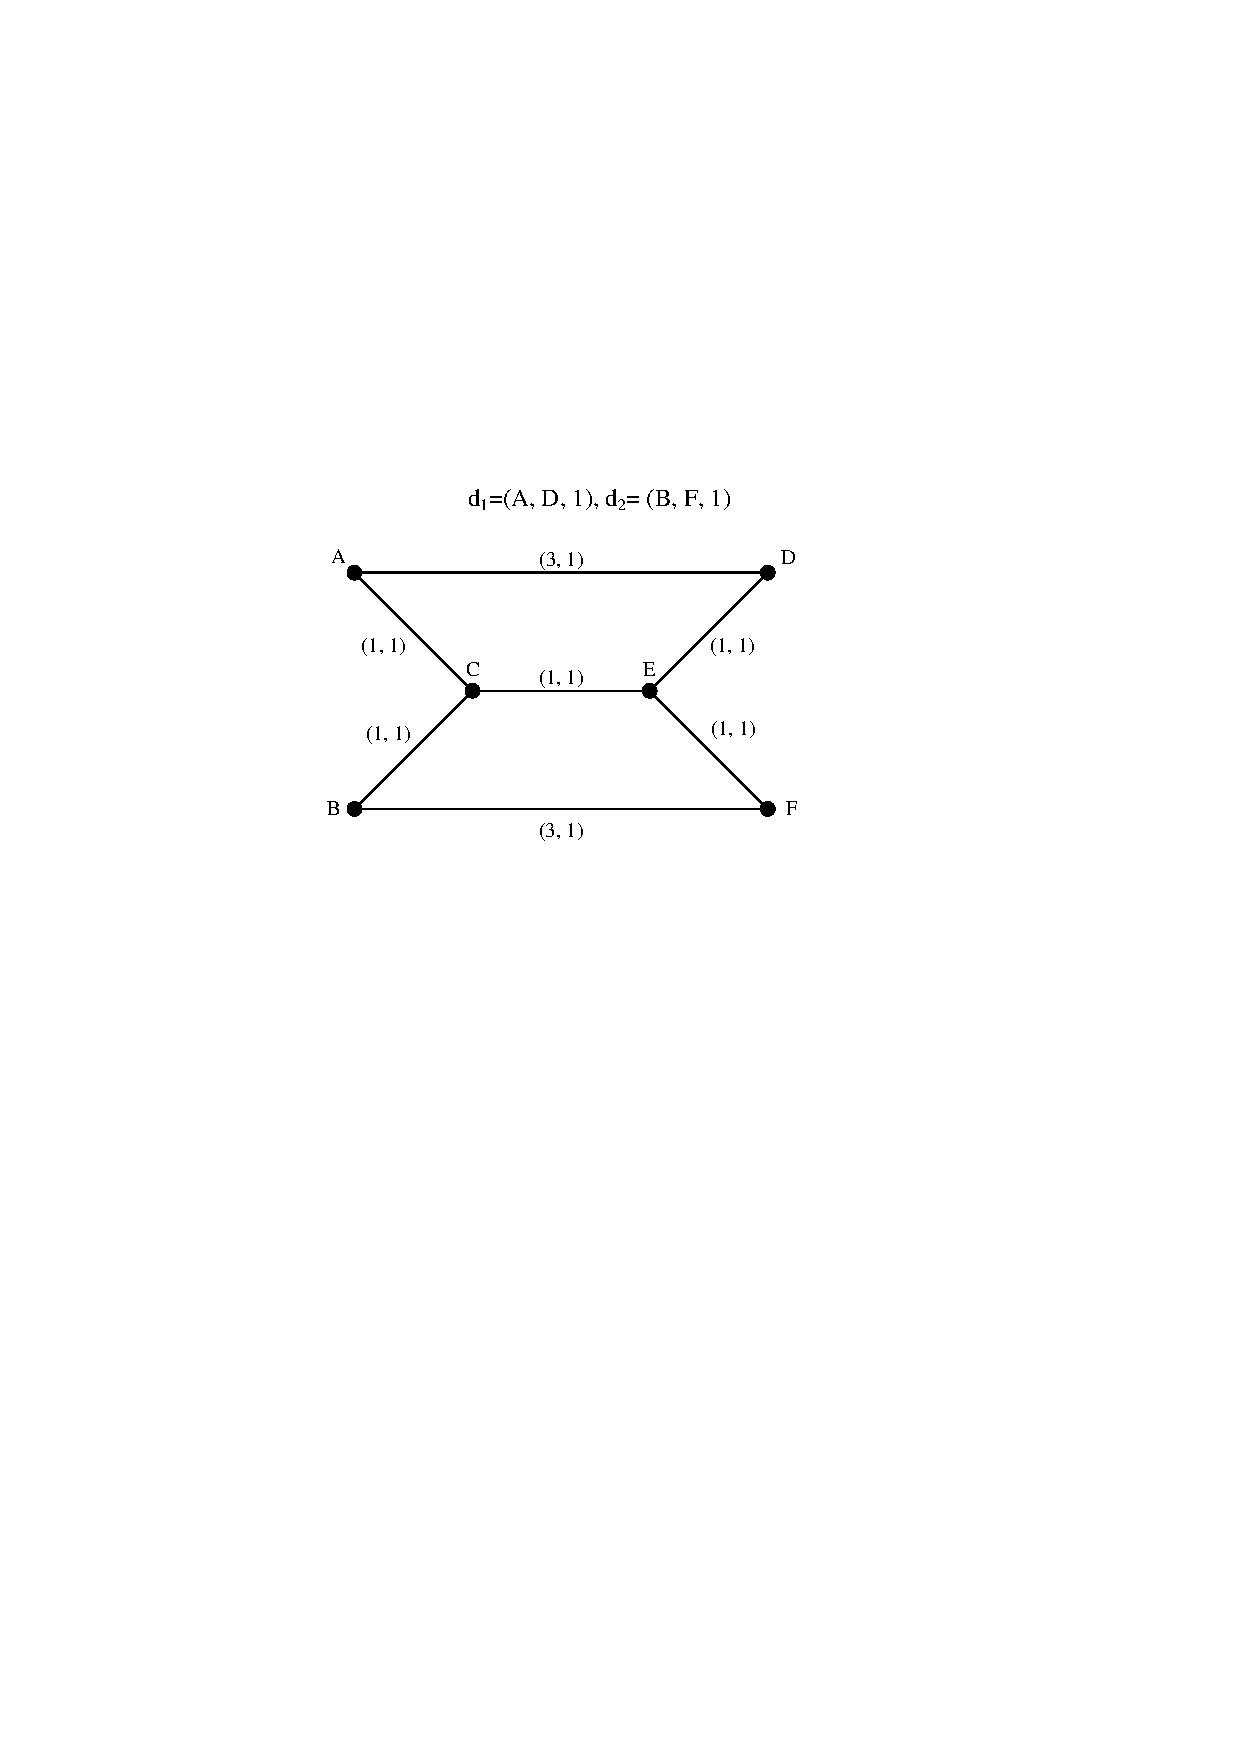
\includegraphics[width=0.4 \textwidth]{figures/PathAdj.pdf}}
\end{center}
\caption{{\footnotesize{路径调整例子}}}
\label{ppt}
\end{figure}

为了说明业务路径调整算法,我们引入一些符号,假设$P$表示步骤2所计算出来的路径集合,其中$p_d\in P$ 表示业务$d$ 的路径; $rp_{d}$ 表示路径$p_d$上的可用带宽,$rp_{d} = min\{r_e | e\in p_d\}$,其中$r_e$ 表示链路$e$上的剩余带宽;$D_l$ 表示剩余业务集合,表示这些业务不能在不违背容量约束的情况下被加入网络中。

路径调整算法如算法\ref{PathAdj}所示。路径调整算法的主要思想是通过调整一小部分业务的路径来得到原问题的优化可行解,算法首先对业务进行排序,这里采用3.3.1.2类似的思想对业务进行排序,一方面,要使得目标函数变小,那些流量需求较大的业务应该优先被加入到网络中,但是如果大流量的业务的路由代价很大,经过了一条很长的路径,就会大量的浪费网络中的链路容量资源,所以算法对当前解中的业务和其路径按照$\frac{\sqrt{bw_d}}{|p_d|}$的值进行排序,其中${bw_d}$代表业务$d$所需要的流量大小,$|p_d|$代表业务$d$的路径$p_d$的代价大小。排序结束后,算法按照顺序试图将业务加入到网络中(第2到9行),如果$rp_d \ge bw_d$,表示业务可以被加入到网络中,那么加入此业务并且更新网络链路的剩余容量值,反之,如果$rp_d<bw_d$,则表示业务选择的路径上的链路容量不足以承载此业务,那么将业务加入剩余集合$D_l$ 中。第2行到第9行的循环结束后,我们得到一个剩余网络$G^{'}(V^{'},E^{'})$,根据前面的讨论,在剩余网络中可能存在一些等价路径,剩余链路中依然有很多可用资源,所以算法重新在剩余网络中为剩余业务$D_l$计算路径(第11到24行)。算法依次遍历集合$D_l$,看能否在剩余网络中为业务寻找一条路径,首先剔除那些链路剩余容量小于业务流量$bw_d$ 的链路,这样保证求出来的路径肯定是满足容量约束的。由于剩余链路是残余网络,所以可能会求出跳数很长的路径,如果跳数太长了,会占用太多的资源,不能达到优化的目的,所以我们对跳数进行约束,如果$|p|/|p_d|<\delta$,则将业务加入到网络中,并更新网络链路容量,否则不加人业务到网络中。虽然这个过程对路径的计算是串行的,但是这个过程是很快速的,这主要有以下原因:第一,由于剩余网络中的链路容量普遍较小,能参与计算的链路很少,对一个剩余业务$d$,在计算路径之前,算法会剔除那些剩余容量小于$bw_d$的链路,所以实际上参与计算的网络拓扑很小;第二,剩余业务量集合$D_l$本身较小;第三,算法越往后面加入业务,可用链路会越来越小,网络会进一步变小。通过这个路径调整算法,可以快速得到原问题的一个优化可行解。
\begin{algorithm}[t]
\begin{algorithmic}[1]
\Require
网络拓扑 $G(V, E)$;
业务量需求集合 $D$;
步骤二算出来的路径集合 $P$;
\Ensure
调整后的路径集合 $AP$;
\State {把业务按照值$\frac{\sqrt{bw_d}}{|p_d|}$进行降序排序}
\For{ $d \in D$}
\If{$rp_{d} \ge bw_d$ }
\State{把路径 $p_d$加入到$AP$中}
\State{在图$G(V,E)$中更新路径$p_d$所经过链路的剩余带宽}
\Else
\State {把业务$d$加入到剩余集合$D_l$中}
\EndIf
\EndFor
\State{$G^{'}(V^{'},E^{'})=G(V,E)$}
\For{ $d \in D_l$}
\State{$G^{''}(V^{''},E^{''})$$=$$G^{'}(V^{'},E^{'})$}
\For{ $e \in E^{'}$}
\If{$r_e< bw_d$}
\State{把链路 $e$ 从图$G^{''}(V^{''},E^{''})$中移除}
\EndIf
\EndFor
\State{在图$G^{''}(V^{''},E^{''})$中为业务$d$计算最短路径$p$}
\If{$\frac{|p|}{|p_d|}\le \delta$}
\State{把路径 $p$ 加入到 $AP$,并把业务从集合$D_l$中移除}
\State{在图$G^{'}(V^{'},E^{'})$中更新路径$p$所经过链路的剩余带宽}
\EndIf
\EndFor
\end{algorithmic}
\caption{路径调整算法}
\label{PathAdj}
\end{algorithm}

\subsection{终止条件}
LR-PTEA的终止条件和GA-PTEA的终止条件一样,假设前$k$次迭代找到的最优解为$B^*$,第$k+1$次迭代找到最优解为$b_{k+1}^*$,如果$b_{k+1}^*<B^*$,那么就更新$B^*=b_{k+1}^*$,如果连续迭代$L$次,$B^*$都不被更新,则判定算法收敛,算法停止。
\section{仿真实验分析}

\subsection {仿真介绍}

为了证明LR-PTEA和GA-PTEA的优化效果,我们把两个算法的优化结果和基于备选路径的MILP模型的最优目标值进行比较,其中每个业务的备选路径数量$K=30$条,我们使用CPLEX \citing{CPLEX}来求解MILP模型,由于CPLEX求解MILP需要很大的计算量,对于大规模的网络,我们无法得到MILP的最优值,因此我们设置了10分钟的求解时间限制,当Cplex求解时间超过10分钟后,我们停止求解,记录Cplex求得的最优可行解和Cplex估计出来的最优下界。

为了观察LR-PTEA和GA-PTEA的加速效果,我们分别设计了两种算法的串行版本LR-STEA和GA-STEA,其中LR-STEA中的路由算法采用带堆优化的dijkstra算法。

我们分别采用ERdos-Renyi (ER) \citing{ER}和 Barab asi-Albert (BA) \citing{BA}两种模型来生成实验网络拓扑,实验中的网络拓扑中点的平均度数为6,网络中的链路代价都是被设置为1。实验中我们随机产生一定数量的业务到达网络,每个业务的的流量大小被设置为1到100之间的随机值。

本文分别比较了各个算法的目标函数,加速效果和算法的收敛性质。GA-PTEA和LR-PTEA中的并行算法都是使用CUDA8.0 进行实现的,跑算法的服务器配置有四个Intel Xeon E5-2630 CPU 和一个 NVIDIA Tesla K40M GPU。

实验中的所涉及到详细参数设置如表\ref{paramter}所示。

\begin{table}[t]
\newcommand{\tabincell}[2]{\begin{tabular}{@{}#1@{}}#2\end{tabular}}
%\setlength{\abovecaptionskip}{-0.5cm}
\centering
\scriptsize{
\renewcommand{\tabcolsep}{0.09cm}
\renewcommand{\arraystretch}{1.2}
\caption{实验参数设置表}
\begin{tabular}{| p{1.2cm} | p{1.2cm} | p{1.2cm} | p{1.2cm} | p{1.2cm} | p{1.2cm} | p{1.2cm} | p{1.2cm} | p{1.2cm} | p{1.2cm} |}
\hline
W&$\delta$&$\phi$&POP&$\alpha$&$\beta$&$\gamma$&m&K&L\\ \hline
50&2&0.15&5000&500&2000&2500&1&30&30\\ \hline
\end{tabular}
\vskip 0.2 cm
\label{paramter}
}
\end{table}

\subsection{目标函数比较}
图 \ref{OB-TA}显示了在点数为1000的网络中,目标函数随着业务数量规模变化的折线图,图中的网络链路容量大小为100。从图 \ref{OB-TA}中我们可以看到目标函数大致随着业务数量呈现线性增加,这和目标函数的表达式相吻合。

从图 \ref{OB-TA}中可以看到LR-STEA/LR-PTEA的优化结果明显优于遗传算法GA-STEA/GA-PTEA的优化结果,这是因为遗传算法提前陷入了局部最优解,导致算法提前结束。

和备选路径MILP模型的Cplex解相比,LR-STEA/LR-PTEA的解明显优于Cplex的解。随着业务数量的增加,LR-STEA/LR-PTEA解和Cplex解的距离逐渐拉开,这是因为Cplex的计算压力随着业务规模的增加而增大,使得Cplex不能在有限时间内找到更好的解。

图\ref{OB-CA}表示的是在容量变化下的目标函数值的变化,其中业务数量为6000,网络链路容量从100到250变化。我们看到,随着容量的增加,目标函数大致呈现线性下降。当链路容量等于250时,LR-PTEA/LR-STEA已经很接近MILP的下界了,这说明LR-PTEA/LR-STEA在网络资源足够时,能很好的优化路由代价。

\subsection{算法时间比较}
图 \ref{TI-ER-TA-1000}和图 \ref{TI-BA-TA-1000}分别列出了各个算法在BA和ER拓扑下的计算时间随着业务数量增加的变化情况,图中拓扑节点数量为1000,业务数量从1000 到6000变化,链路的容量为100。由于各种算法的时间差距过大,我们用三种不同的尺度进行展示。首先,Cplex的时间限制都为10分钟,所以我们不再列出来。

在图\ref{TI-ER-TA-1000}和图 \ref{TI-BA-TA-1000}中,我们可以看到GA-PTEA相对于GA-STEA加速比可达到20倍以上,但是由于遗传算法本身收敛较慢,所以GA-PTEA的计算时间还是很糟糕的。

观察图 \ref{TI-ER-TA-1000}和图 \ref{TI-BA-TA-1000},我们发现LR-STEA和LR-PTEA的时间曲线会发生大幅度的波动,这是因为算法的迭代次数变化较大。根据3.4.5的讨论,在连续$L$次没有寻找到更优解后,LR-PTEA/LR-STEA就会停止,我们把$L$设置为30。其实$L$设置得偏小了,算法有可能会找到更好的解,但是这些解的下降程度很小(通过收敛图 \ref{LR-CO},可以看到算法在前30次内下降幅度较大,后面的下降幅度很小),所以为了优化整体时间,我们设置迭代次数为较小的30次,这样可能会使得算法提前结束,从而导致算法的迭代次数变化幅度较大。

观察图 \ref{TI-ER-TA-1000}和图 \ref{TI-BA-TA-1000},我们发现随着业务数量的增加,LR-PTEA的加速优势变大。总体来看,LR-PTEA相对与LR-STEA有平均12倍的加速。


图 \ref{TI-BA-NO}和图 \ref{TI-ER-NO}表示算法计算时间随着网络拓扑大小的变化情况,其中到达网络的业务数量为网络拓扑点数目的4倍,可以看到随着网络拓扑变大,计算时间也相应增加,GA-PTEA的计算时间不管在小拓扑还是大拓扑下都远远大于LR-PTEA 的计算时间。拓扑较小时LR-PTEA相对与LR-STEA的加速很小,但随着网络拓扑规模的增加,LR-STEA的计算时间大幅上升,而采用GPU加速计算的LR-PTEA上升幅度较小,网络拓扑达到一定规模后LR-PTEA对LR-STEA有较大的加速优势。
\vspace{0.8cm}
\begin{figure}
\setlength{\abovecaptionskip}{-0.5cm}
\begin{center}
{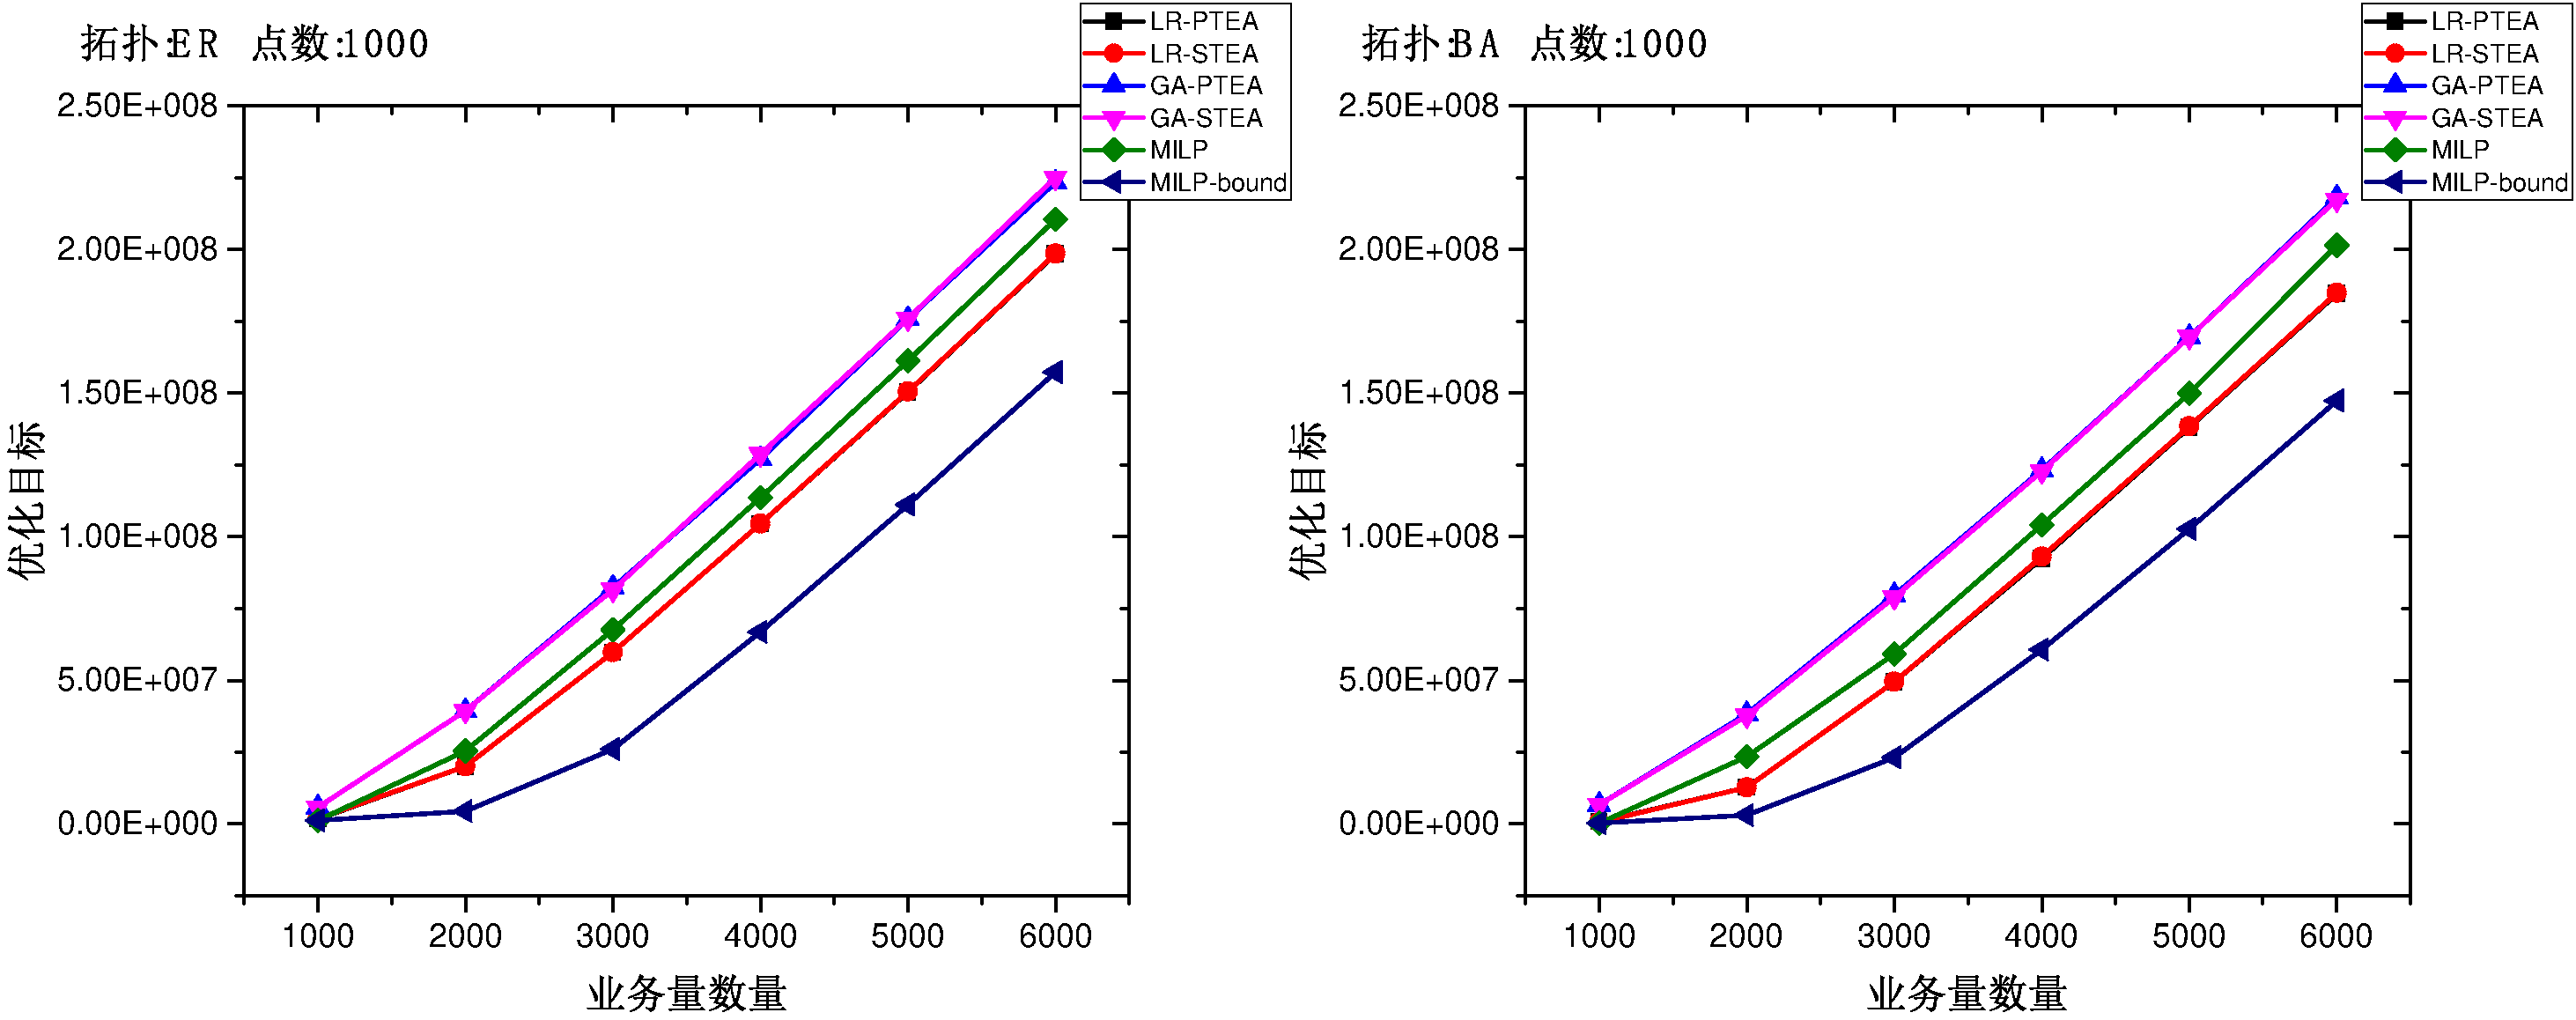
\includegraphics[width=0.8 \textwidth]{figures/OB-TA.pdf}}
\end{center}
\caption{{\footnotesize{目标函数值随业务数量变化示意图}}}
\label{OB-TA}
\end{figure}
\begin{figure}
\vspace{-0.2cm}
\setlength{\abovecaptionskip}{-0.5cm}
\begin{center}
{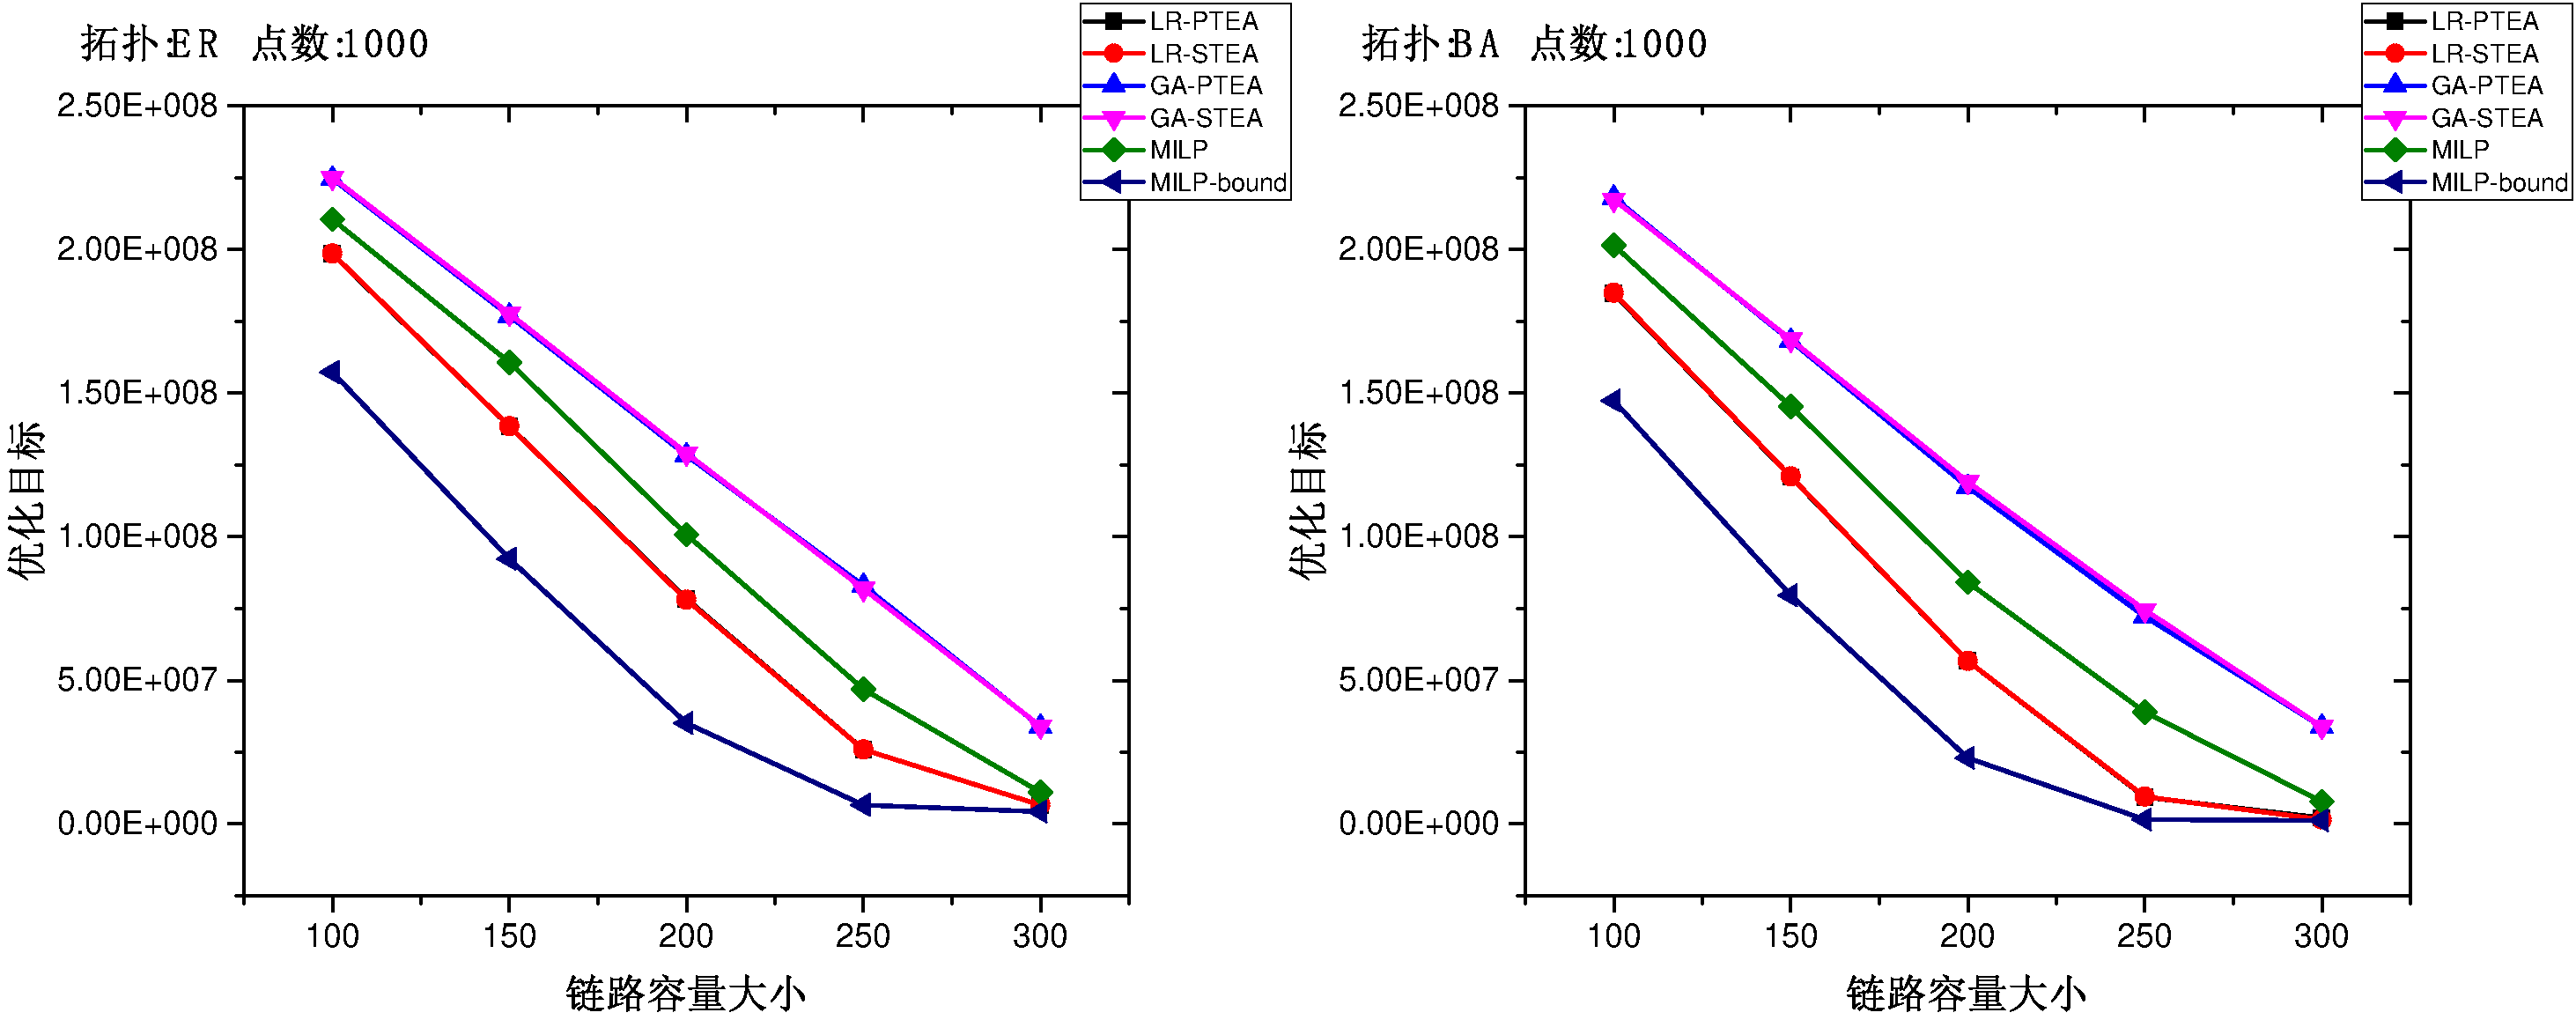
\includegraphics[width=0.8 \textwidth]{figures/OB-CA.pdf}}
\end{center}
\caption{{\footnotesize{目标函数值随链路容量变化示意图}}}
\label{OB-CA}
\end{figure}

\begin{figure}
\setlength{\abovecaptionskip}{-0.5cm}
\begin{center}
\vspace{-1cm}
{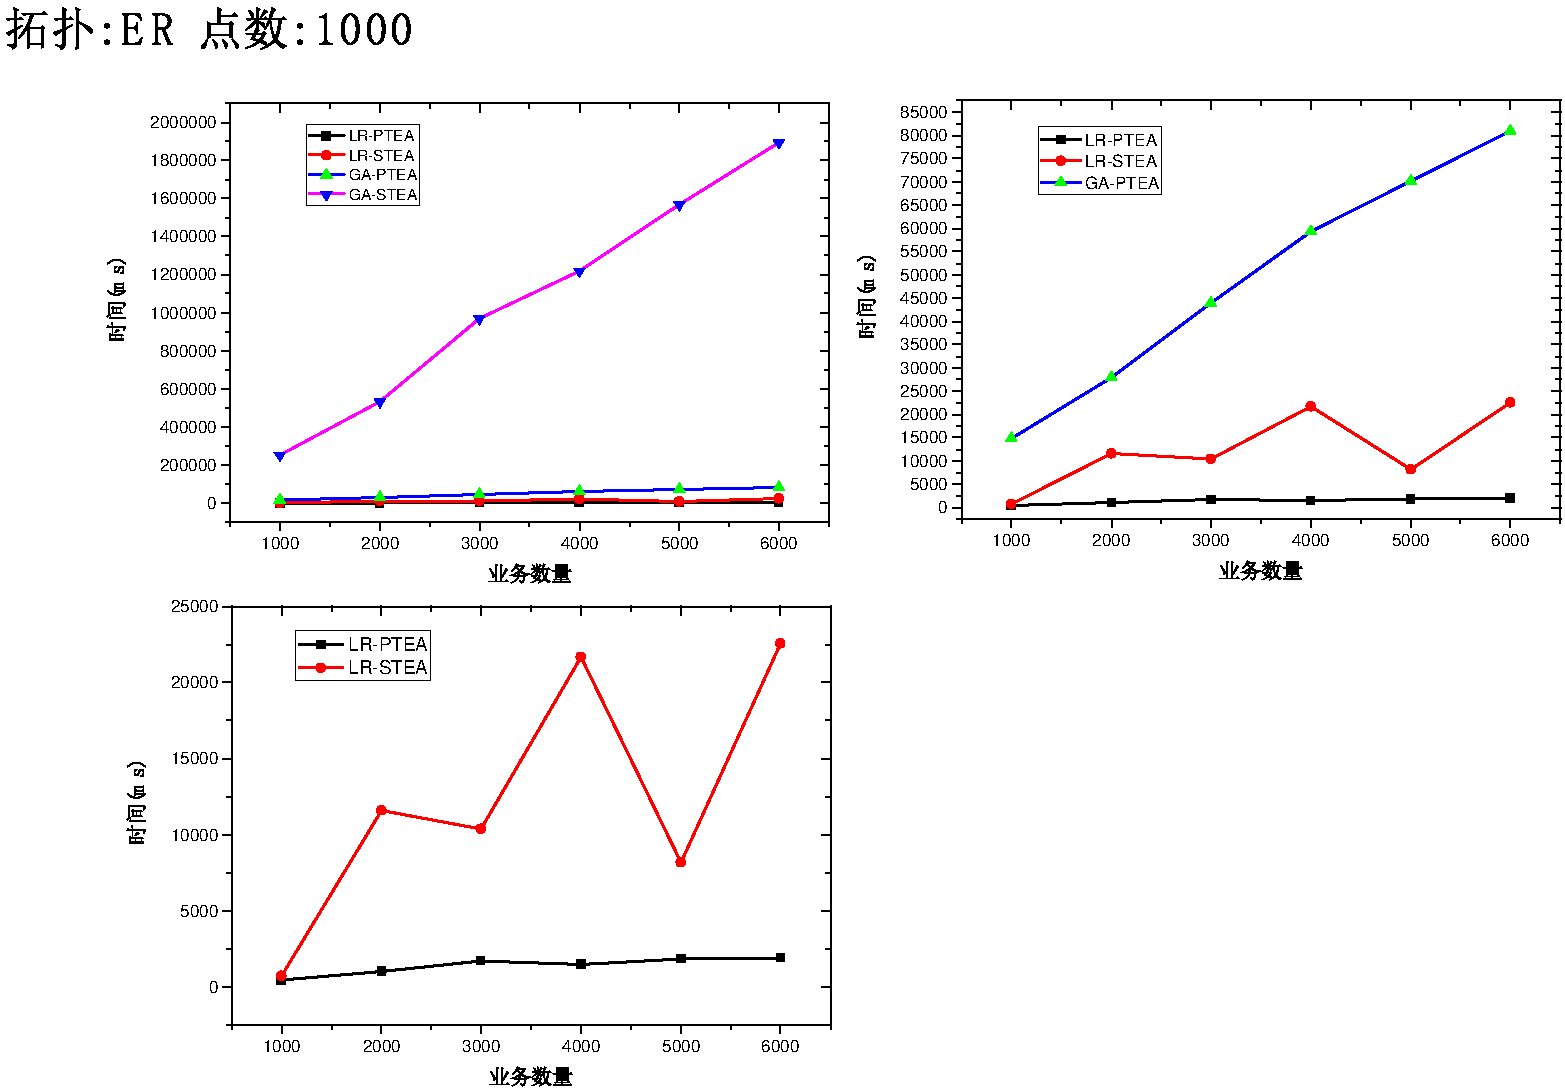
\includegraphics[width=0.9\textwidth]{figures/TI-ER-TA.pdf}}
\end{center}
\caption{{\footnotesize{计算时间随业务数量变化示意图(ER)}}}
\label{TI-ER-TA-1000}
\end{figure}
\begin{figure} 
\vspace{-2cm}
\setlength{\abovecaptionskip}{-0.5cm}
\begin{center}
{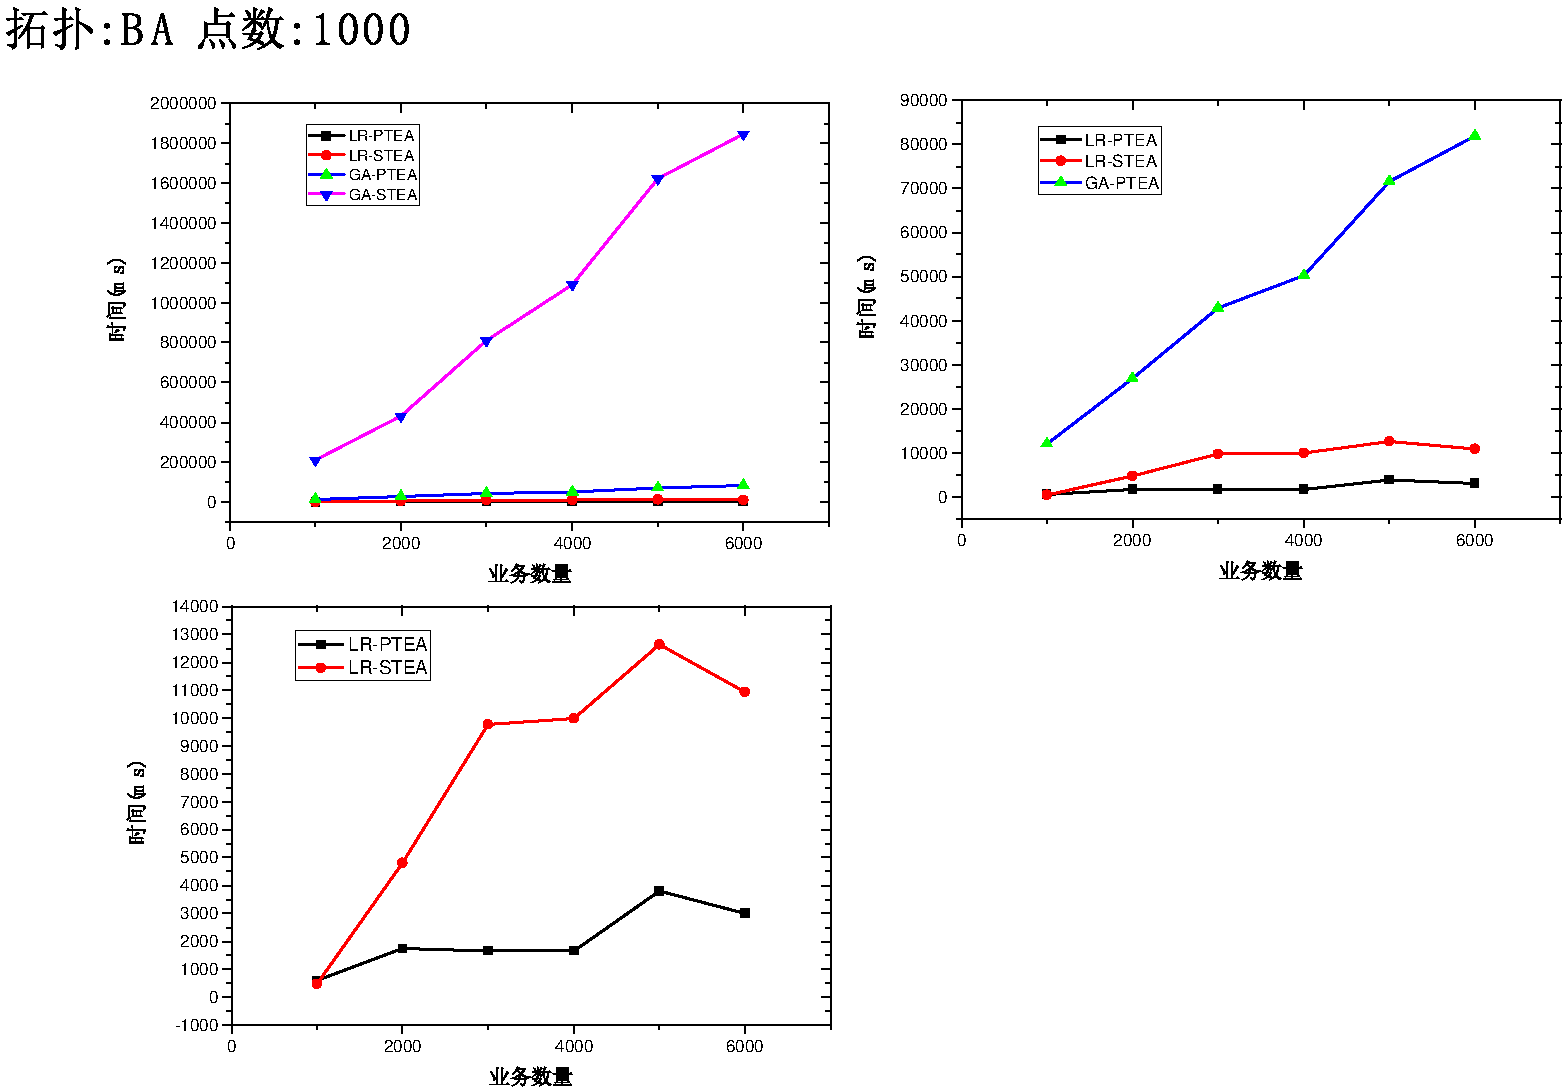
\includegraphics[width=0.9\textwidth]{figures/TI-BA-TA.pdf}}
\end{center}
\caption{{\footnotesize{计算时间随业务数量变化示意图(BA)}}}
\label{TI-BA-TA-1000}
\end{figure}



\begin{figure}
\setlength{\abovecaptionskip}{-0.5cm}
\begin{center}
{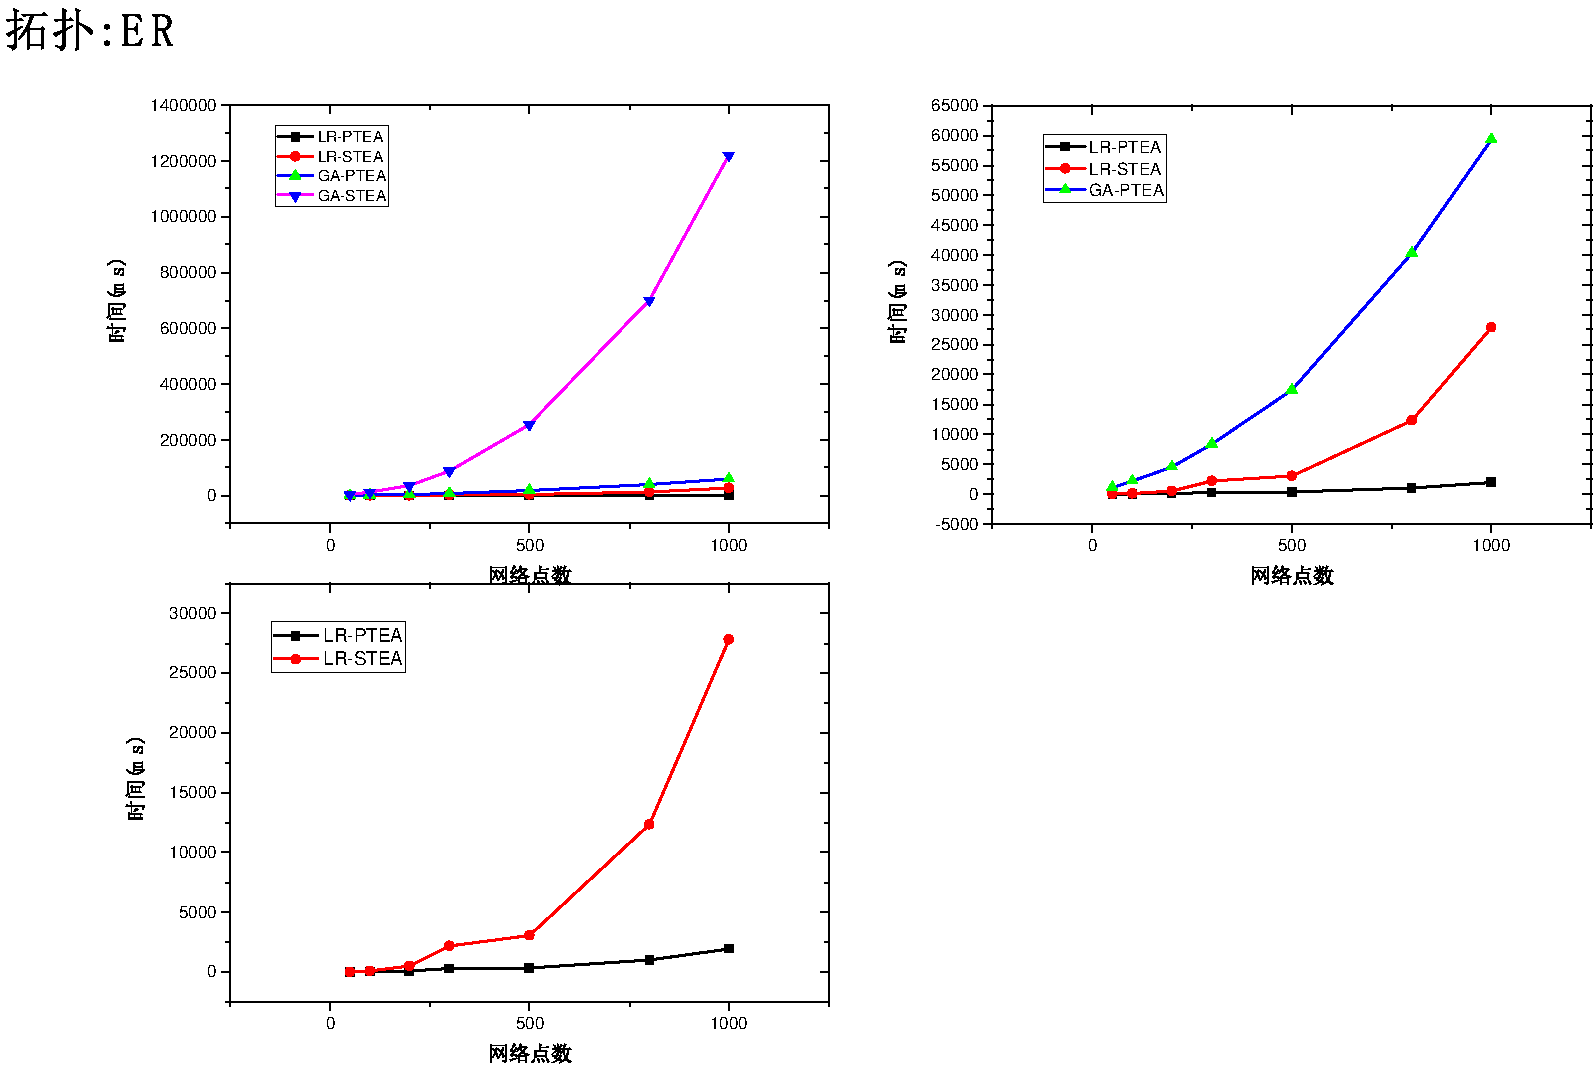
\includegraphics[width=0.8\textwidth]{figures/TI-ER-NO.pdf}}
\end{center}
\caption{{\footnotesize{计算时间随拓扑大小变化示意图(ER)}}}
\label{TI-BA-NO}
\end{figure}
\subsection{算法收敛性}
图 \ref{GA-CO} 和图 \ref{LR-CO}分别是GA-PTEA和LR-PTEA的收敛过程图。可以看到遗传算法的初始值较差,迭代次数较多,而且最终陷入到了局部最优解,而LR-PTEA第一次的解已经很好,这是因为LR-PTEA不是基于备选路径的,他会通过路径调整策略为业务重新寻找路径,从而得到一个较好的初始目标值。LR-PTEA的目标函数值在很短的迭代次数里快速下降,但是LR-PTEA的曲线不够平滑,说明算法的波动较大,收敛终止条件不好控制,这也是图 \ref{TI-ER-TA-1000}和图\ref{TI-BA-TA-1000}产生波动的原因。

\section{本章总结}
本章研究了SDN IP网络下的并行业务量工程算法,首先提出了新的业务量工程代价函数,建立了业务量工程模型,设计了两种基于GPU的并行优化算法方案GA-PTEA和LR-PTEA,我们的实验发现GA-PTEA的加速比可达20倍以上,LR-PTEA的加速比能达到10倍以上,LR-PTEA能够在短时间内得到目标函数的优化解。

\begin{figure}
\vspace{-0.2cm} 
\setlength{\abovecaptionskip}{-0.5cm}
\begin{center}
{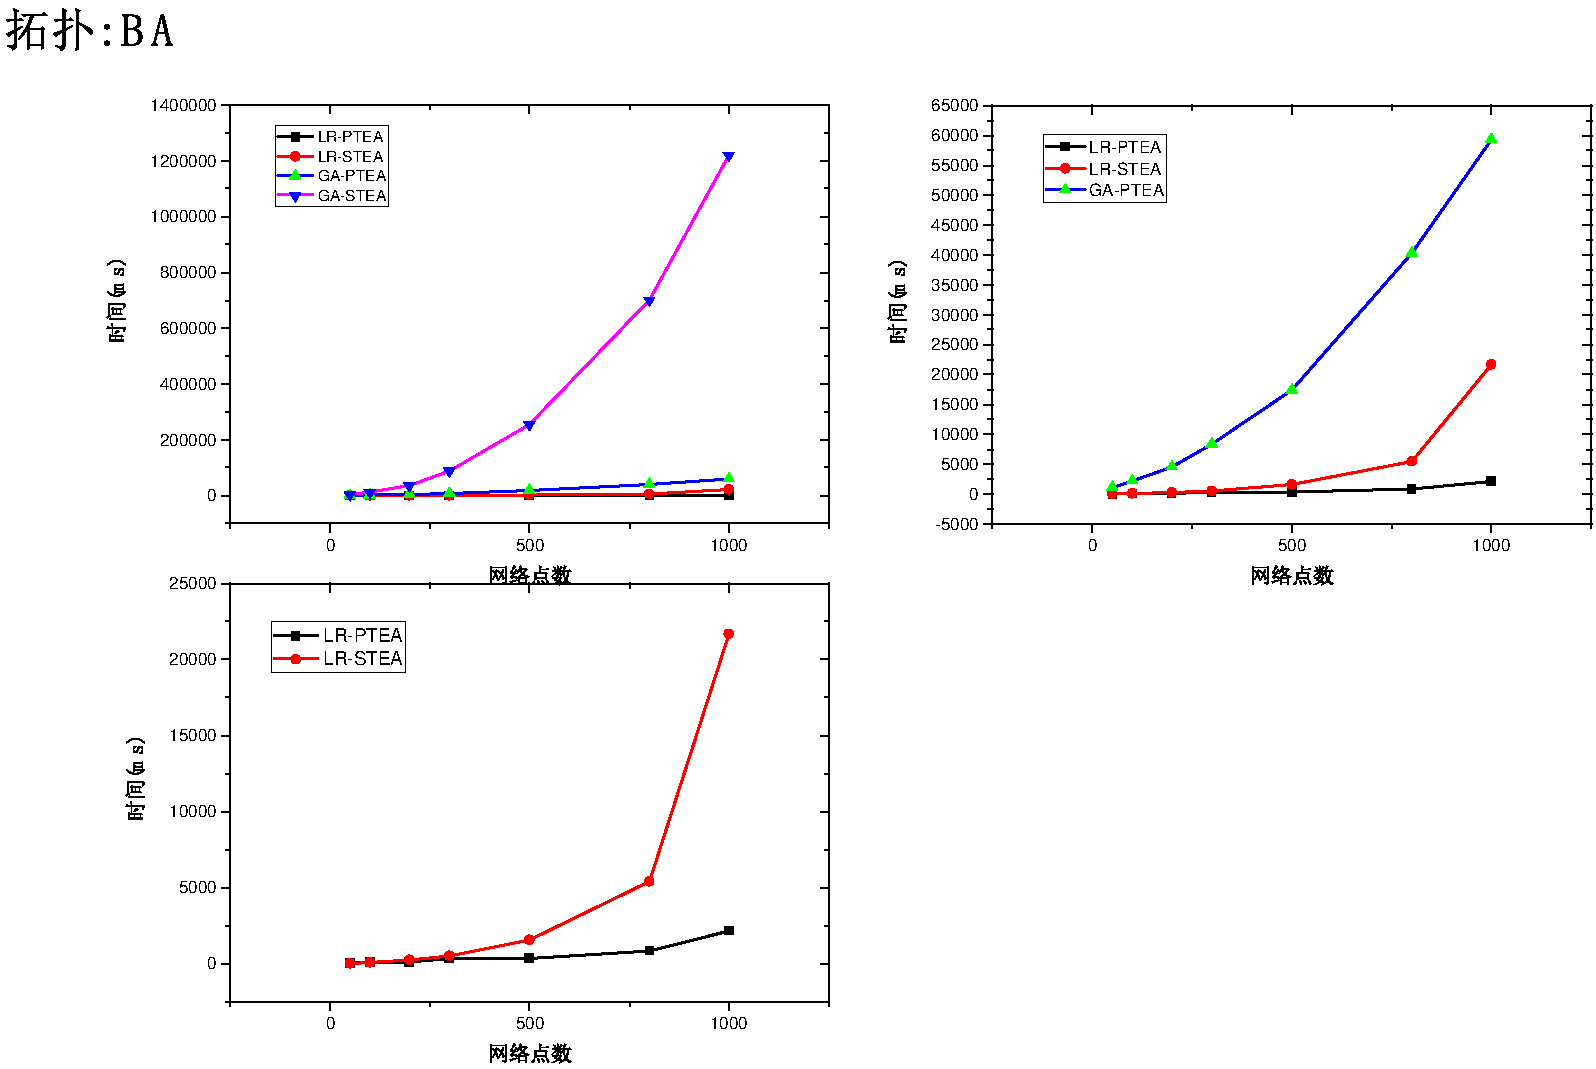
\includegraphics[width=0.8\textwidth]{figures/TI-BA-NO.pdf}}
\end{center}
\caption{{\footnotesize{计算时间随拓扑大小变化示意图(BA)}}}
\label{TI-ER-NO}
\end{figure}
\begin{figure}
\vspace{-0.2cm} 
\setlength{\abovecaptionskip}{-0.5cm}
\begin{center}
{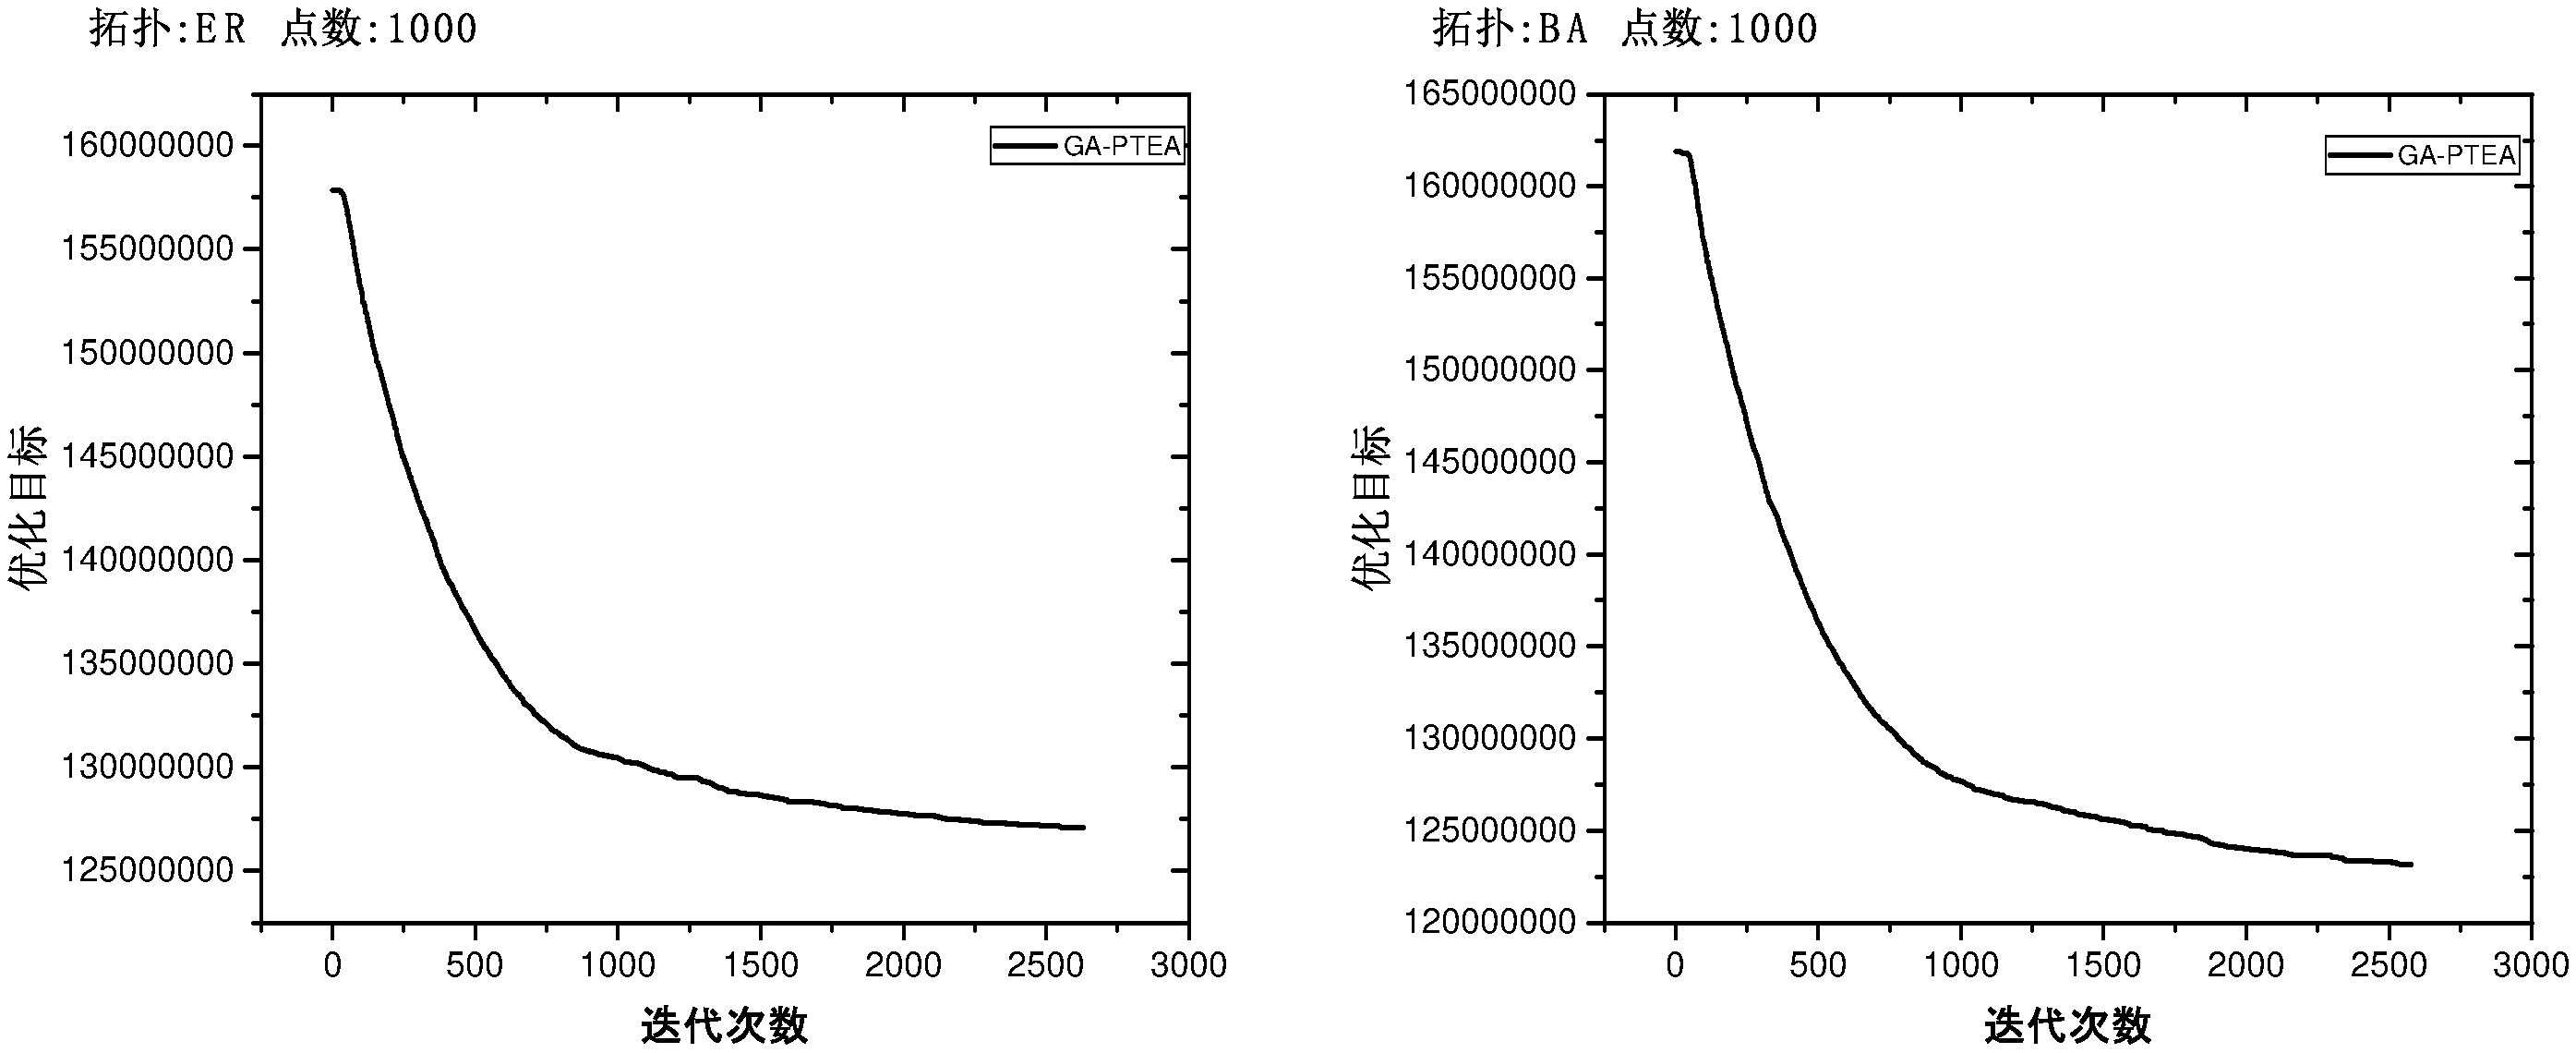
\includegraphics[width=0.8\textwidth]{figures/GA-CO.pdf}}
\end{center}
\caption{{\footnotesize{GA-PTEA 收敛性}}}
\label{GA-CO}
\end{figure}
\begin{figure}
\setlength{\abovecaptionskip}{-0.5cm}
\begin{center}
{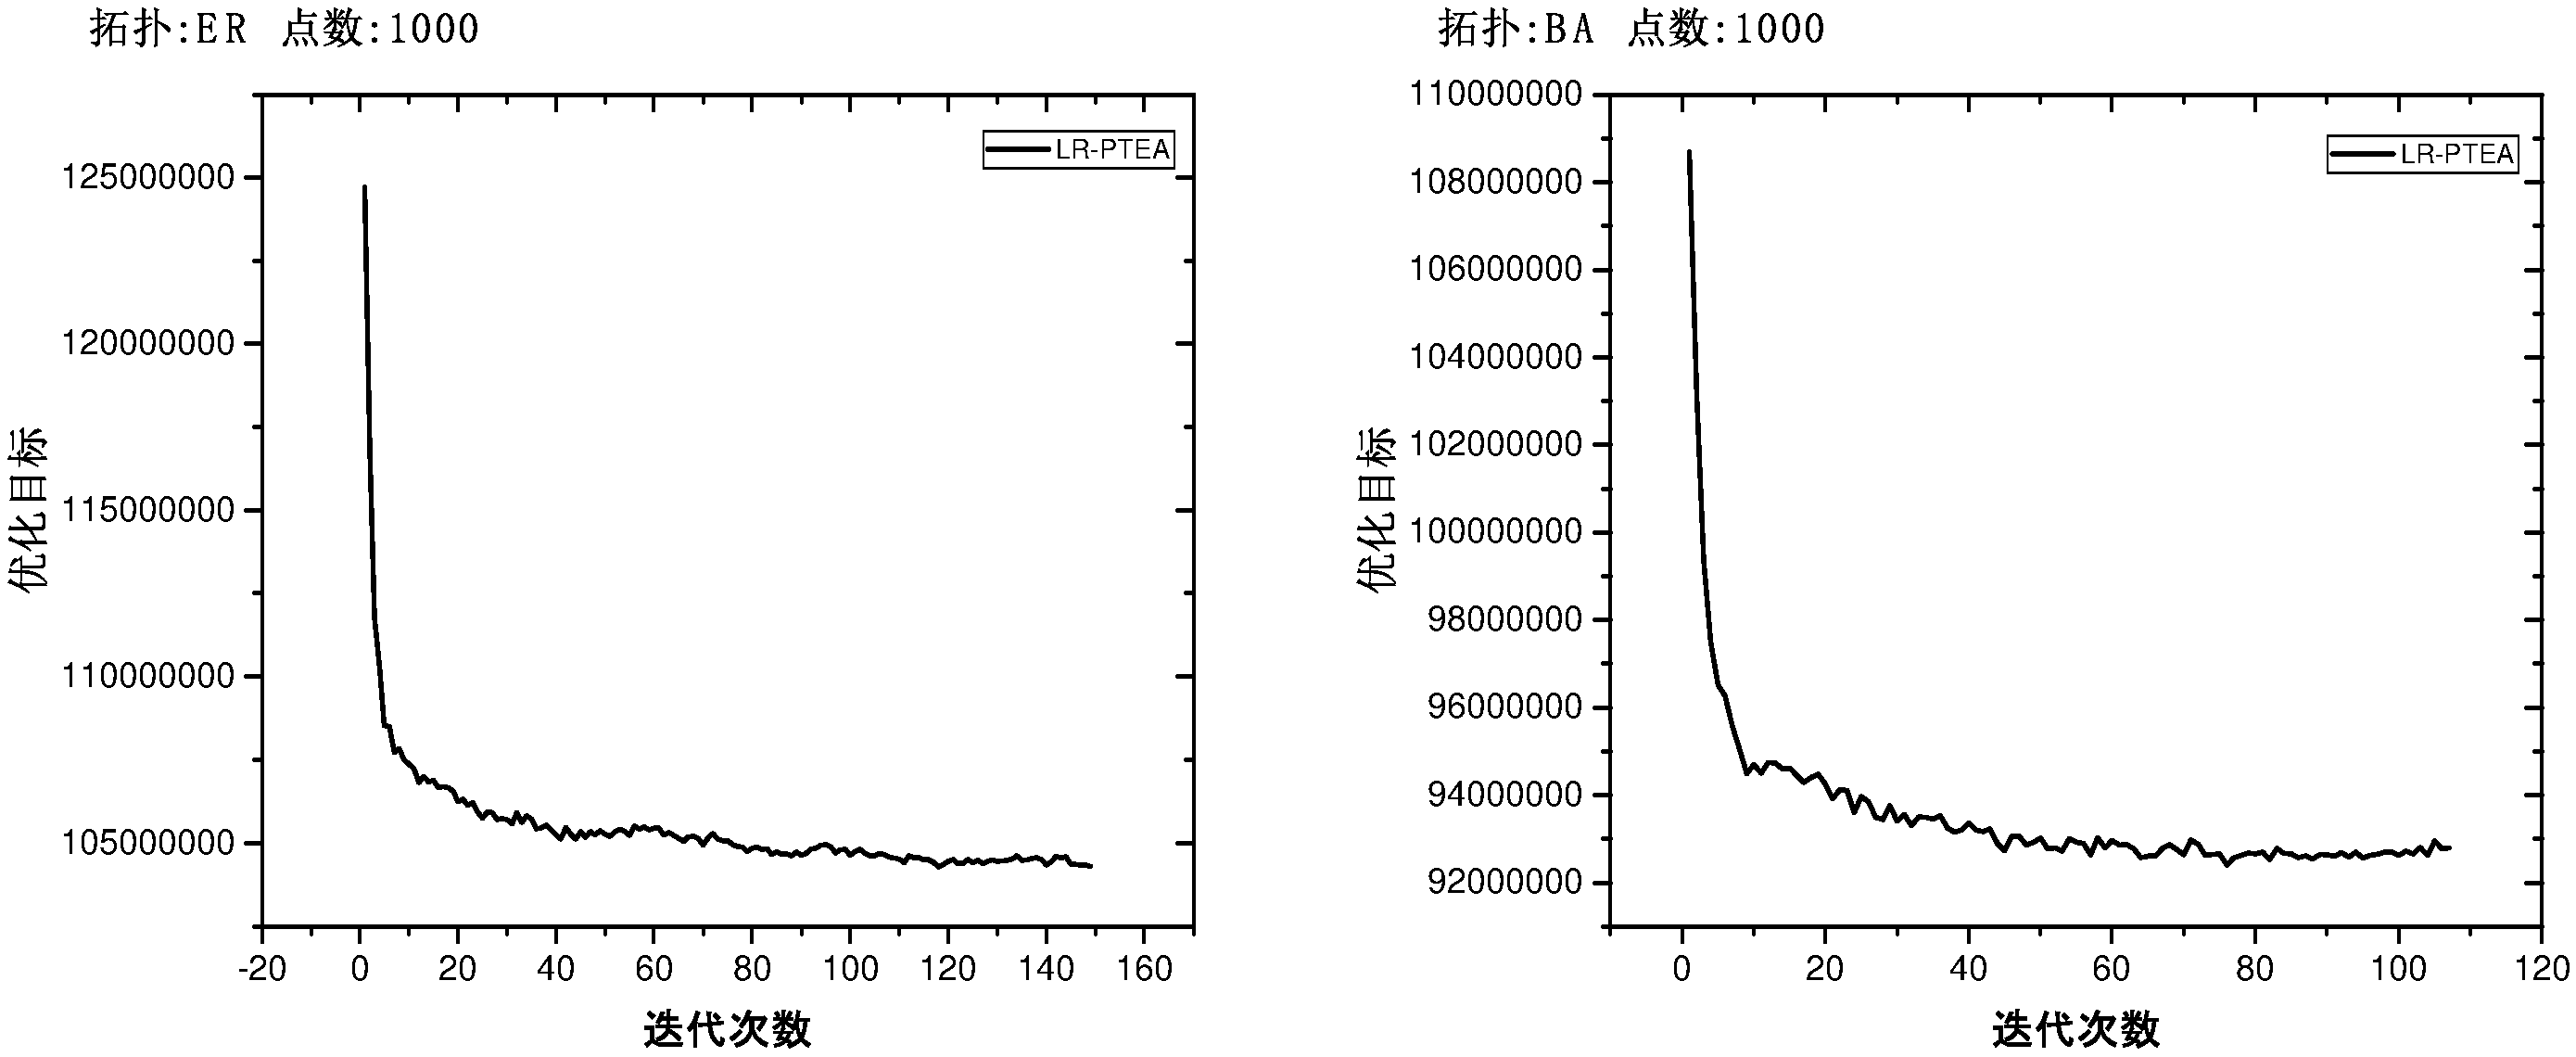
\includegraphics[width=0.8\textwidth]{figures/LR-CO.pdf}}
\end{center}
\caption{{\footnotesize{LR-PTEA 收敛性}}}
\label{LR-CO}
\end{figure}







% !Mode:: "TeX:UTF-8"

\chapter{SDN弹性光网络下的并行业务量工程算法研究}
\section{引言}
在EON架构中,存在细粒度的带宽间隙(比如,12.5GHZ),他比WDM网络所遵循的ITU-T的带宽间隙粒度(50GHZ或者100GHZ)要小很多,而且,这些带宽间隙可以根据需要被组合在一起以提供更宽的通道。为了提高带宽利用率,在EON中存在混合速率,每个速率的业务需要不同数量的频谱间隙数量。理论上,EON能够灵活地提供各种速率,但是在实际中,EON却可能只含有很少的速率种类,这主要是因为:第一,随着数率种类的增加,频谱碎片和管理复杂度将显著增加。第二,实际的EON已经从较低的线路数率升级到更高的线路数率,并存大量速率的情况已经很少见了。

为了在EON网络中加入业务,控制平面必须在网络中找到一条路径,同时,还需要在此路径上的链路上分配足够的频谱带宽,来创建一个合适的端到端光路连接,这被称为路由和频谱分配(Routing and Spectrum Allocation,RSA)问题,RSA问题可以进一步分为静态RSA问题和动态RSA问题。静态的RSA问题出现在网络规划阶段,其中流量需求是已知的,这样可以离线计算出最优或者接近最优的RSA解。动态RSA问题是指在实时业务情况下光通路的路由选择和波长分配的优化问题。在动态RSA问题中,业务随机的到达和离开光网络,造成网络频谱资源实时变化,而且当业务到达网络时,控制平面需要在短时间内找到合适的路径来安排业务。所以,动态RSA问题比静态RSA问题更具有挑战性。

本章考虑在EON中解决动态场景下的业务量工程问题,我们采用分层图模型将频谱分配问题简化为路由选择问题,设计出基于分层图模型的频谱分配与业务量工程算法(Traffic Engineering and Spectrum Allocation Algrithm,TESAA),在进行频谱分配的同时优化路由代价。针对无权图和带权图两种情况设计基于GPU的并行路由算法来加速TESAA。实验发现,基于GPU并行的PTESAA(parallel TESAA)算法对串行算法STESAA(serial TESAA)的加速比可达到5倍。我们将TESAA和基于分层图模型的贪心算法比较,发现TESAA在短时间内能够大大地优化路由代价,并且由于路由代价减小,占用的网络资源较少,最终使得网络阻塞率降低。
\section{分层图模型}
当业务到达网络时,SDN控制器需要找到可行的路径,并且为路径分配合适的频谱资源。由于EON的物理限制,业务路由需要满足以下约束:

第一,传输跳数限制:光信号的传输质量会随着传输跳数的增加而下降,为了在目的点顺利恢复光信号,光链路的传输跳数需要小于一个阈值$W_{max}$。

第二,频谱连续性限制:每条光连接的频谱从它的源节点到它的目的节点 ,在所经过的链路上保持不变。

第三,频谱不重叠限制:同一光纤链路中的频谱不能分配给不同的光路。

第四,频谱邻近限制:频谱邻近约束保证分配给一个光路径的频谱必须是一个连续的部分。

论文 \citing{ELAYER}中提出一种分层图(Layered Graph)模型来解决WDM网络中的路由和波长分配问题,分层图模型将路由选择和波长分配问题统一到一起来,使得路由和波长分配问题变得简化,这种分层图模型也可以很容易推广到EON的RSA问题中。

我们使用有向图$N(V,E)$表示物理网络拓扑,其中$V=\{v_1,v_2,...,v_N\}$表示节点集合,$E=\{e_1,e_2,e_3,...,e_M\}$表示边集合,$e_k=(i_k,j_k)$表示边的头节点为$v_{i_k}$,边的尾节点为$v_{j_k}$。假设所有光链路具有相同的频谱范围$W=(F_{start},F_{end})$, 其中$F_{end}-F_{start}=C$。EON所支持的速率集合为$R$, 比如,$R={40Gb/s,100Gb/s,400Gb/s}$,每一种速率$r\in R$需要一个特定的频谱宽度$b_r GHz$。一个源节点为$s$,目的节点为$t$,速率为$r Gb/s$的业务被表示为$TD(s,t,r)$。

下面我们讨论分层图的产生过程,假设第一个速率的为$r$的业务$TD(s,t,r)$到达网络,我们从可用的频谱切割出一块频谱大小为$b_r$ 的连续带宽分配给速率为$r$ 的业务,假设这块频谱的起始频率为$fs_{( r,1 )}$,终止频谱为$fe_{( r,1 )}$,那么$fe_{( (r,1) )}-fs_{( (r,1) )}=b_r$。我们把物理链路上的频谱范围为$( fs_{( (r,1) )},fe_{( (r,1) )} )$的部分从链路上切割下来,把切割下来的部分组成一个新的虚拟网络$N^{( r,1) )} ( V^{( (r,1) )},E^{( (r,1) )}) )$,在这个新的网络中每条链路的频谱范围都是$(fs_{( (r,1) )},fe_{( (r,1) )})$,这样切割下来之后,原来的物理网络的频谱范围更新为$( F_{start}+b_r,F_{end} )$。如果在这个切割出来的图$N^{( r,1) )} ( V^{( (r,1) )},E^{( (r,1) )}) )$上为业务求一条最短路径$p$,那么容易知道路径$p$一定满足约束2、3、4,这样问题被简化为单纯的路由问题。要注意的是,这个虚拟图上的频谱不能再分配给其他速率为$r'$ 的业务$TD(s',t',r')$,即使$b_{r'}<b_r$,因为这样会产生大量的频谱碎片,使得频谱利用率下降。所以这些分割出来给速率$r$的频谱,将继续被分配给速率为$r$的业务。当下一个速率为$r$的业务$TD (s'',t'',r)$ 到达网络时,他首先在图$N^{( r,1) )} ( V^{( (r,1) )},E^{( (r,1) )}) )$中寻找路径,如果找到合适的路径,则业务被加入网络并且更新路径经过的链路的可用频谱为0。反之,如果他在图$N^{( r,1) )} ( V^{( (r,1) )},E^{( (r,1) )}) )$中没有找到合适的路径,那么算法会重新去切割频谱得到虚拟网络$N^{( r,2) )} ( V^{( (r,2) )},E^{( (r,2) )}) )$,这样随着大量业务的动态到达和离去,会产生大量的虚拟图,频谱资源已经大量地分布在各个虚拟图中,我们把这些虚拟图叫做分层图(Layered Graph)。

图 \ref{layer}展示了分层图的组织结构,原图被切割成一个分层图集集合$L$,$L_i \in L$表示速率$i$的分层图集合。速率$r$一共有$|L_r|$个分层图,速率$r$的第$l$个分层图占用频谱$(fs_{( (r,l) )},fe_{( (r,l) )})$。图 \ref{layer}中,点$v_i^{( (r,l) )}$表示速率$r$的第$l$层图上的第$i$号点。
\begin{figure*}
\setlength{\abovecaptionskip}{-0.5cm}
\begin{center}
{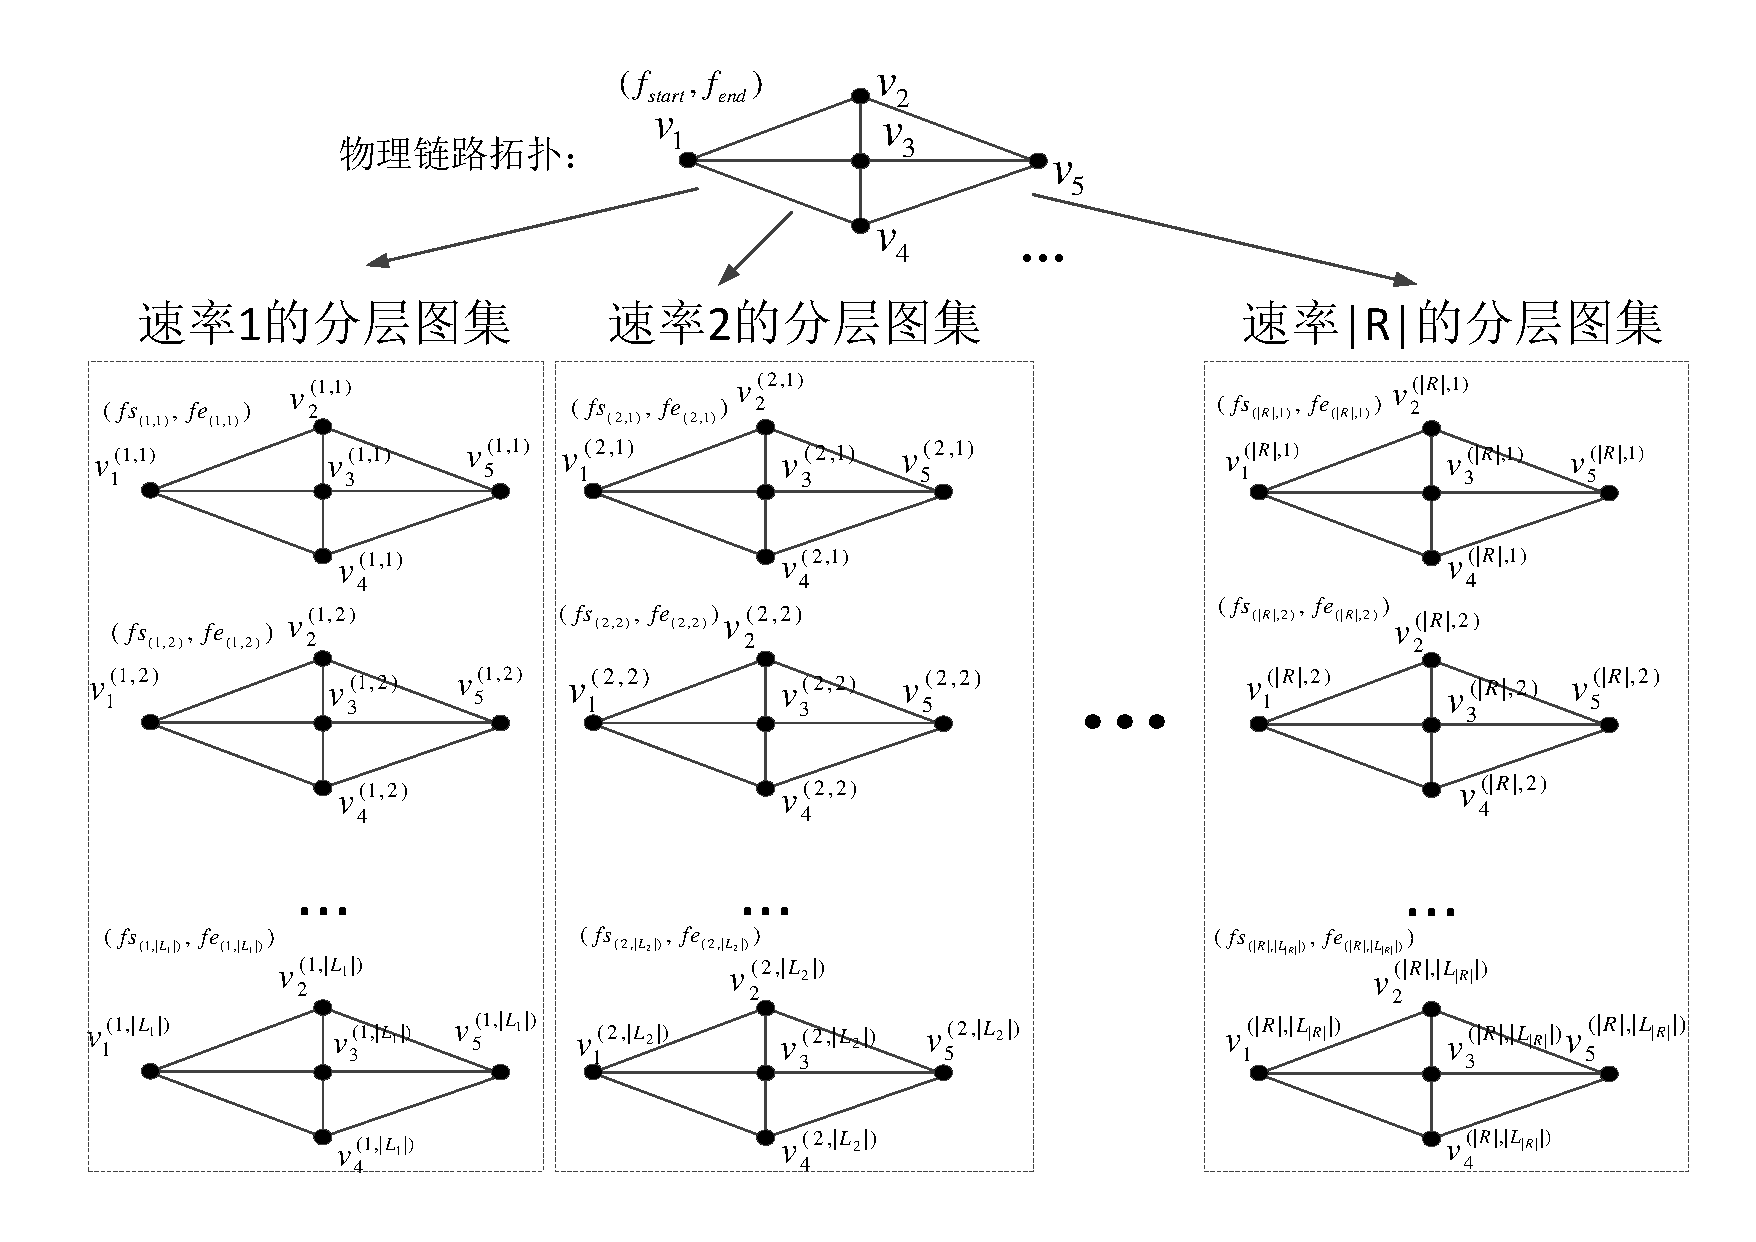
\includegraphics[width=1 \textwidth]{figures/LAYER.pdf}}
\end{center}
\caption{{\footnotesize{分层图组织结构示意}}}
\label{layer}
\end{figure*}
\section{分层图模型下的业务量工程算法}
根据前面的讨论,当一个速率为$r$的业务$TD_r(s,t)$到达网络时,一共有$L_r$ 个分层平面都可以用于此业务,也就是说如果在这些图当中都能为业务找到合适的路径的话,那么业务就有$L_r$ 条路径可供选择,我们可以选择代价最小的一条来优化路由。进一步,当有一批速率为$r$ 的业务集合$D_r$到达网络时,如果大家都选择同一层加入的话,会出现大量的冲突,而且路由代价也会很大,但是现在对每一个业务都有多个分层图平面可以选择,这就给路由代价的优化提供了可能,不同的业务可以选择不同层上的路径来进行路由,以使得总体路由代价减小,节省网络频谱资源,从而优化阻塞率。

根据以上讨论,本节提出一个基于分层图模型的频谱分配与业务量工程算法(TESAA,Traffic Engineering and Spectrum Allocate Algrithm),算法在进行频谱分配的同时对业务的路由代价进行优化,算法流程如图 \ref{bblayer}所示。
\begin{figure*}
\vspace{-1cm}
\setlength{\abovecaptionskip}{-0.5cm}
%\setlength{\belowcaptionskip}{-0.5cm}
\begin{center}
{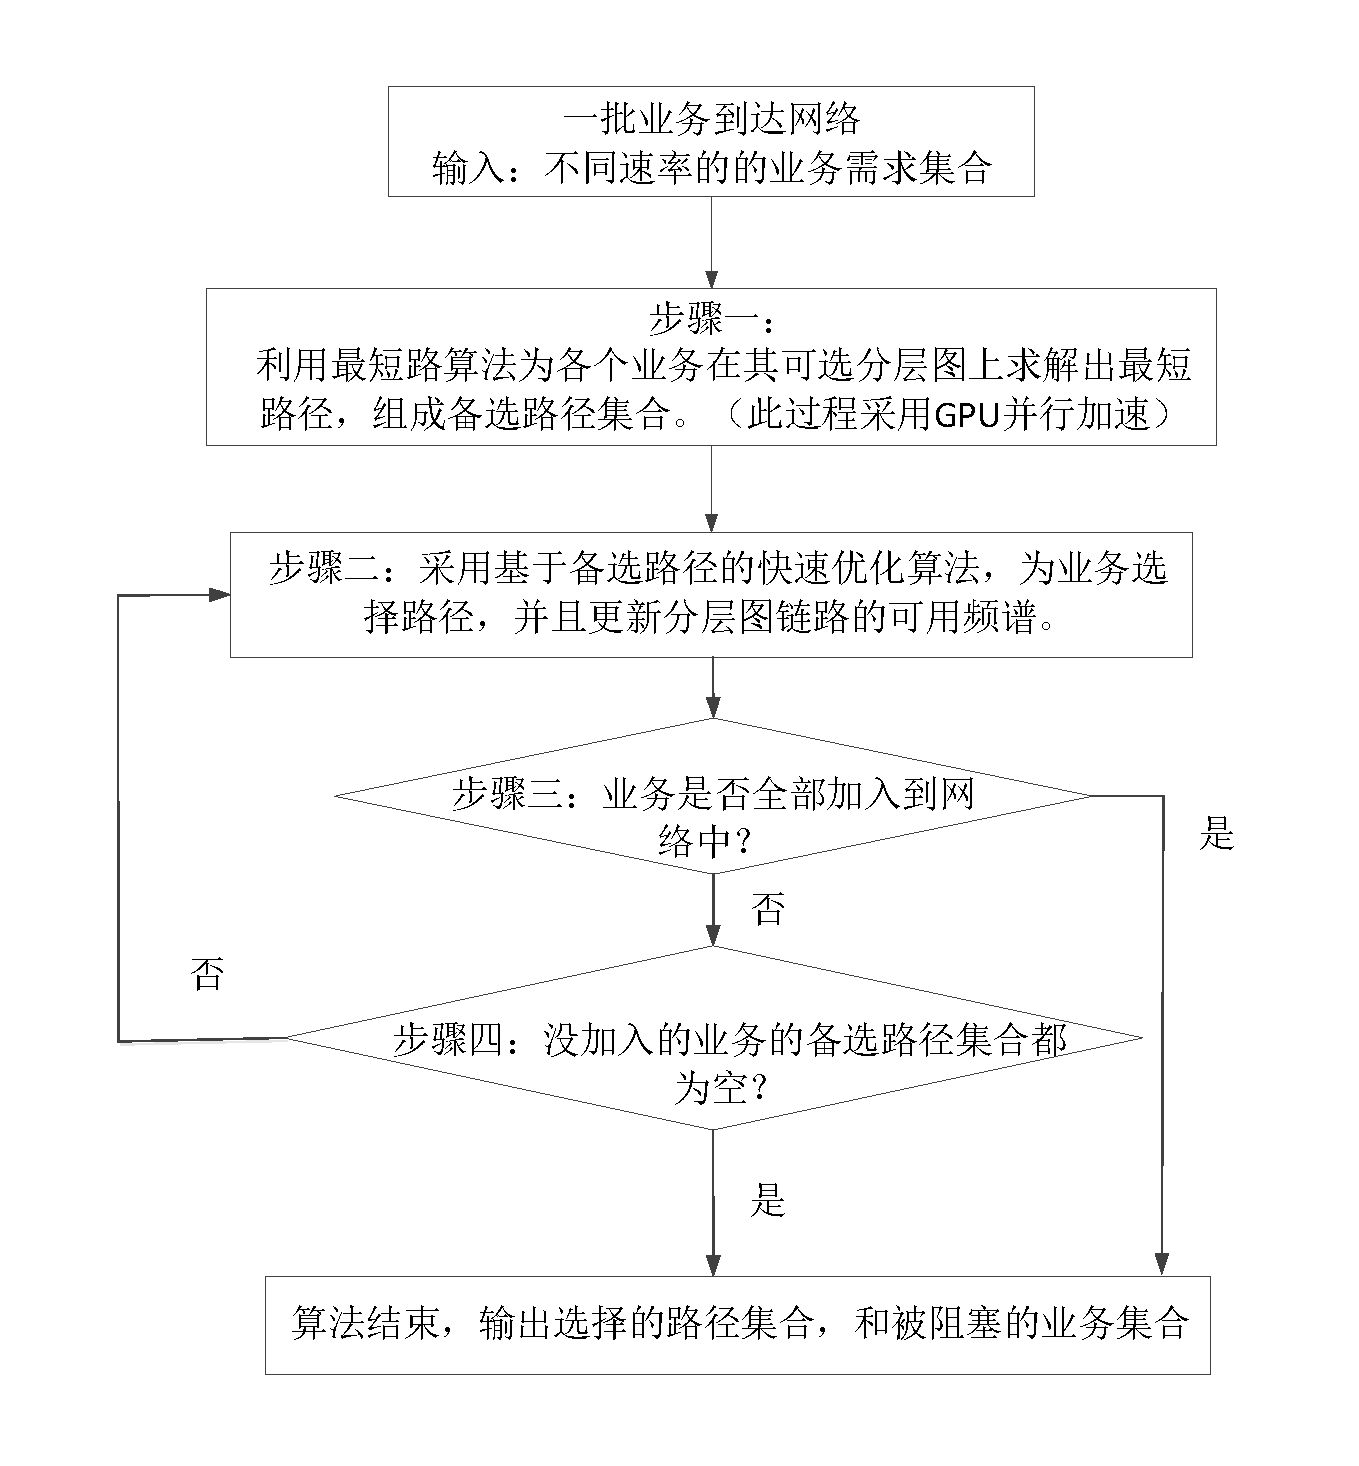
\includegraphics[width=0.9\textwidth]{figures/bbprocess.pdf}}
\end{center}
\caption{{\footnotesize{算法优化流程}}}
\label{bblayer}
\end{figure*}

当一批业务到达网络时,算法会对每一个业务在其所有可用分层图上计算路由,这个过程的计算量较大。但是不同业务之间是独立的,不同分层图之间也是独立的,所以可以采用并行算法来进行加速设计,4.4和4.5将讨论无权图和有权图上的并行路由算法来加速这个步骤。当备选路径都求出来了之后,我们采用一种快速路径选择算法来把业务安排进网络,这个步骤采用一种简单的贪心算法,实验发现这种简单的贪心算法可以很好的优化路径代价。当业务的路径确定后,如果每个业务都能加入到网络,那么本轮算法结束,如果还有剩余的业务没有被安排进网络,需要判断业务的备选路径集合是否为空,如果为空,则说明所有层都不能为业务求出路径,业务将被阻塞。反之,如果业务的备选路径集合不是空,则说明业务是因为和其他业务的路径冲突而导致不能被安排进网络的,分层图中可能还存在其他可用路径,所以需要重新在分层图中计算路径,算法回到步骤二,对这些业务进行重新计算。

步骤一的具体算法将在4.4和4.5介绍,这里介绍步骤二的快速优化算法,快速优化算法的主要思想是在备选路径集合中为每个业务选择路径以使得整体路径代价最小,在动态环境下需要在短时间内安排好路径,所以为了提高计算速度,这里采用一种简单但快速的贪心算法来进行解决,算法如\ref{arrange}所示。
\begin{algorithm}[htb]
\begin{algorithmic}[1]
\Require
$N(V,E)$:分层图;
$P$:备选路径集合;
$D$:业务需求集合;
\Ensure
$AP$:加入业务的路径集合;
\For{$T \in D$}
\State {对$P_T$中的路径按照路径的代价进行升序排序}
\EndFor
\State {对$D$按照每个业务的最小路径代价进行升序排序}
\For{$T \in D$}
\For{$p \in P_T$}
\If{路径$p$所对应分层图上的相应链路没有被占用}
\State{把$p$加入到$AP$中,并更新$p$所对应的分层网络上的链路。}
\State{\bfseries break}
\EndIf
\EndFor
\EndFor
\end{algorithmic}
\caption{路径选择算法}
\label{arrange}
\end{algorithm}

算法开始时对每个业务的备选路径按照其代价进行升序排序,也就是每个业务优先会选择代价较低的备选路径。然后,再对业务按照其最小代价的路径进行升序排序,这样保证优先考虑代价较小的业务。然后,算法依次加入业务到网络,对每一个业务,遍历其已经排序好的备选路径,如果在对应分层图上路径所包含的链路都是空闲的,则加入业务到网络中,更新分层图上的相应链路为占用状态,把这个路径$p$ 加入到集合$AP$ 中,最后算法输出路径集合$AP$。
\section{无权图情况下的GPU算法设计}

无权图情况下,路由的代价就是路径的跳数,跳数越少说明占用的网络资源越少,尽量优化路径的跳数可以节省网络资源,进一步的降低动态情况下网络的阻塞。无权图情况下的路由算法一般使用BFS (宽度优先搜索)算法进行求解,BFS 算法从离目的节点最近的点开始,一层一层的进行扩展直到找到目的节点,每扩展一层跳数增加一跳,每扩展一层就需要遍历大量的边,这些边的扩展操作是相互独立的,所以为算法提供了并行设计的可能性,在加上不同分层图上的路由计算是相互独立的,所以总体并行粒度是很大的。下面分别对不同并行层次的设计进行讨论。
\subsection {相同速率业务的并行}

如图\ref{bfs}所示,对速率都为$r$的一批业务,算法并行地在每个分层图上进行路由计算,在各个分层图上,具有相同源节点的业务组成业务组,因为他们的路径可以一起计算。对每一个业务组,在GPU 上开辟$|E|$个线程对每一条边进行扩展操作,那么整个过程的的并行粒度为$|L_r|\times|D_r|\times|E|$,其中$|D_r|$为速率为$r$的业务组数量。
\begin{figure*}
\setlength{\abovecaptionskip}{-0.5cm}
%\setlength{\belowcaptionskip}{-0.5cm}
\begin{center}
{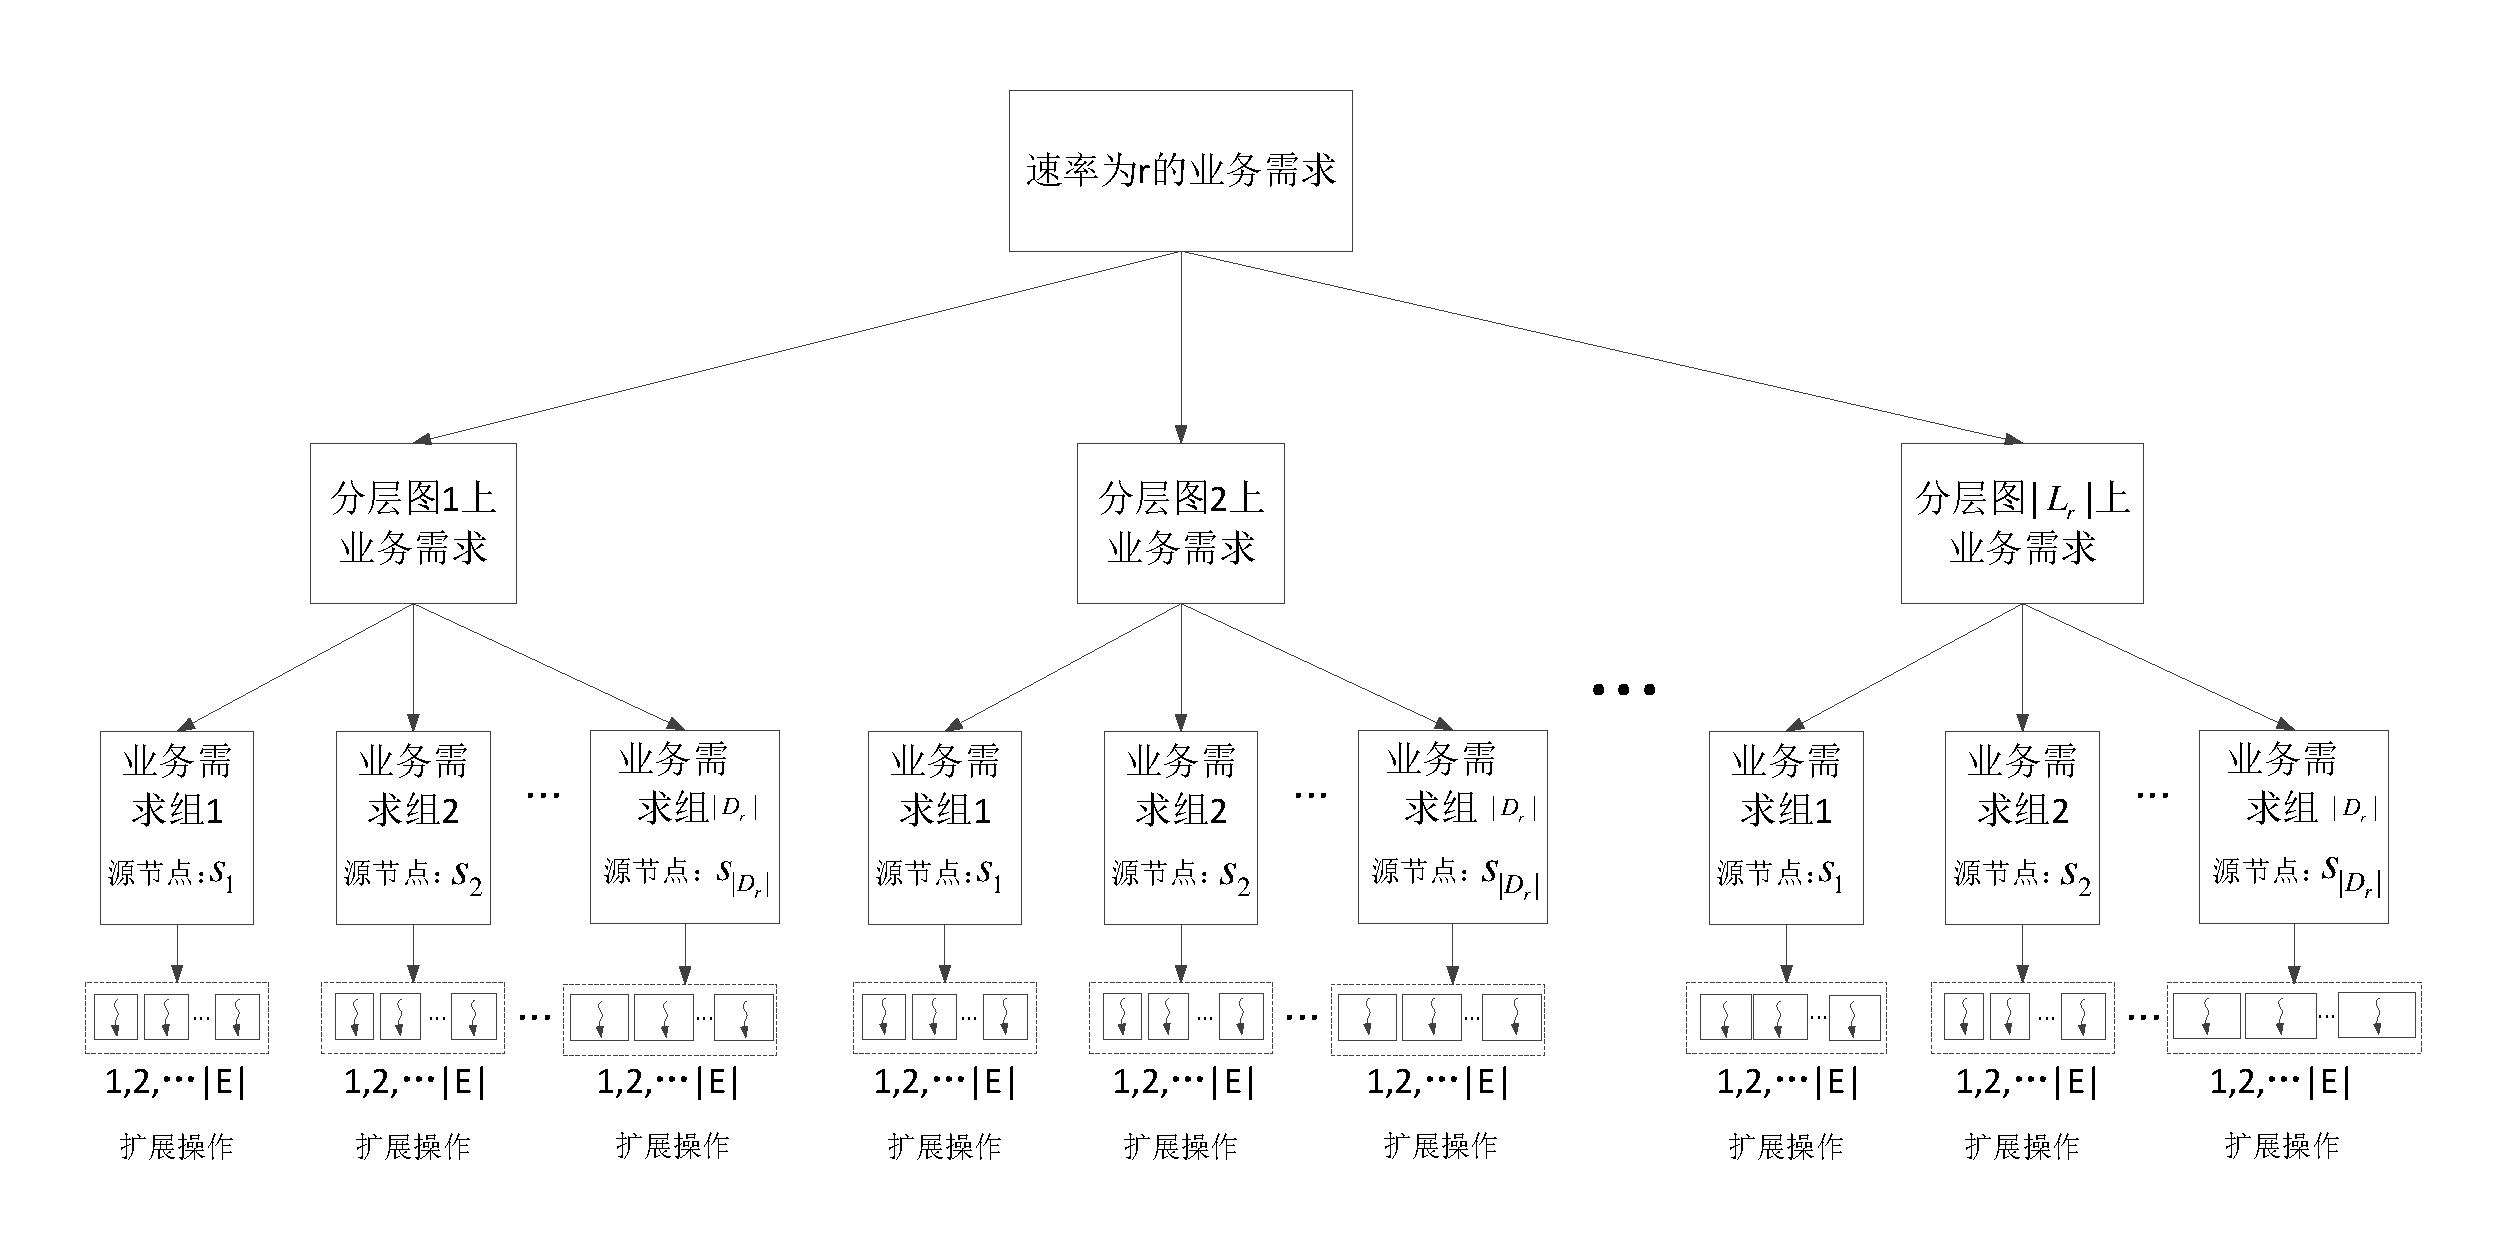
\includegraphics[width=1 \textwidth]{figures/bfs.pdf}}
\end{center}
\caption{{\footnotesize{相同速率业务的BFS并行示意图}}}
\label{bfs}
\end{figure*}
\subsection{不同速率间业务的并行}
由于动态业务情况下每次到达网络的不同数率的业务数量是变化的,不同速率之间业务的并行不容易直接实现在一个kernel中,我们可以把不同速率的业务路由计算抽象成不同的任务,所以本文采用CUDA提供的流并行进行并行设计,如图 \ref{bfssteam}所示。
\begin{figure*}
\setlength{\abovecaptionskip}{-0.5cm}
\begin{center}
{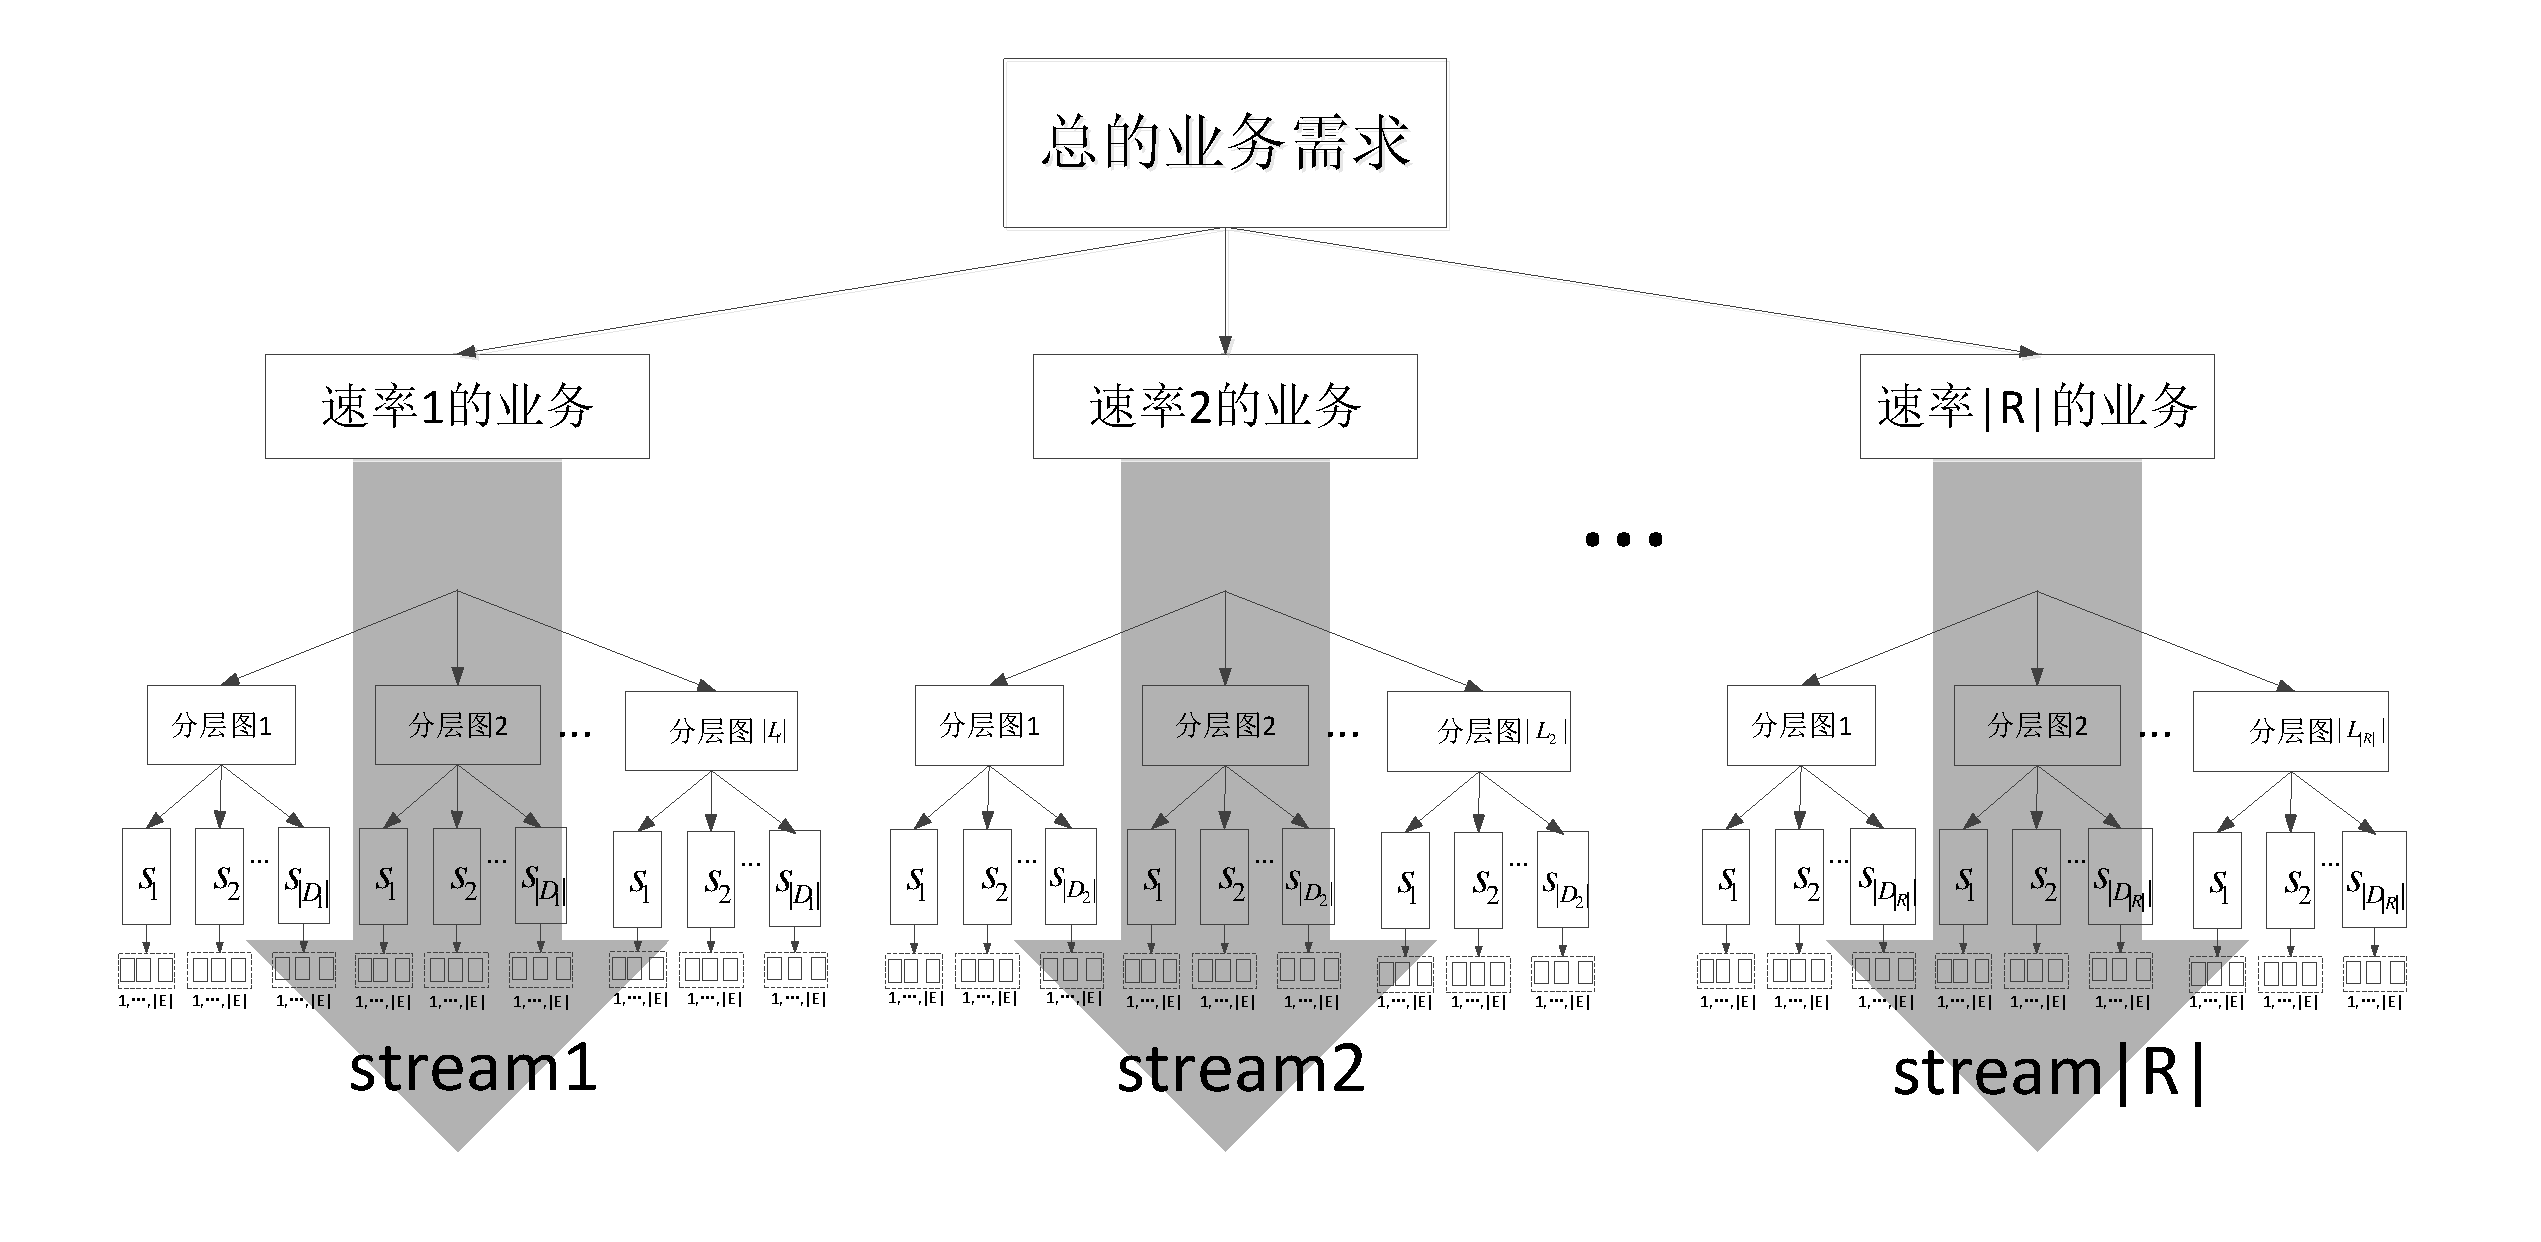
\includegraphics[width=1 \textwidth]{figures/hbfs.pdf}}
\end{center}
\caption{{\footnotesize{BFS流并行示意图}}}
\label{bfssteam}
\end{figure*}

我们为每一个速率建立一个流来负责这个速率的业务计算,假设一共有$|R|$个不同的速率,那么需要建立$|R|$个流,多个流同时切换执行,充分利用GPU的SM资源,当SM资源足够时,不同流的kernel将并行执行,当SM不足时,不同的kernel之间可以进行快速的切换,以达到隐藏延迟的效果。这样,算法的总体并行粒度达到$|L_r|\times|D_r|\times|E|\times|R|$。

\subsection{GPU上的kernel设计}
和3.4.2中讨论的不一样,在BFS的并行中不会存在前驱节点更新的同步问题。但是,我们依然需要两个kernel函数,这是因为扩展操作需要执行多次,如果扩展和更新被放在一个kernel函数,那么更新也会执行多次,这会增加内存的访问,所以我们把两个操作分成两个kernel,一个$kernel\_BFS\_extend$进行边的扩展操作,一个$kernel\_BFS\_update$进行前驱节点的更新操作,其中$kernel\_BFS\_extend$需要多次调用,但是$kernel\_BFS\_update$只需要在最后执行一次。

在$kernel\_BFS\_extend$(见算法\ref{Kernelex})中,输入$E$是所有的分层图的边所组成的集合,$Dist$是预先分配的距离标记数组,他是一个三维数组,第一维表示当前距离数组对应的分层图标号,第二维度表示源节点,第三维度表示目的节点,比如$Dist[3][10][5]=4$表示在第3个分层图上,点10到5的距离为4。初始时,除了源节点距离被初始化为0之外,其他的距离都被初始化为无穷大。$rid$表示当前kernel 负责计算的业务速率标号,他是区分不同流的标记,$rid$不同表示执行kernel的流不同。$round$ 表示当前扩展的层数,由于BFS是一层一层地进行扩展操作的,我们需要记录当前层数来决定哪些边需要扩展。算法开始时先进行一系列映射操作,将线程映射到边标号$eid$,当前所在分层图标号$lid$,以及源节点标号$sid$。 由于动态情况下,边的可用状态可能发生变化,找到边之后,需要判断这条边是否可用,如果不可用则返回。接着判断当前边是否可以进行扩展操作,如果边$e$的目的节点($e.head$)已经被更新过了($Dist[lid][sid][e.head] \le round$),则不能再更新了,反之,还需要判断边$e$的出发节点$e.tail$是否是上一次扩展层的节点($Dist[lid][sid][e.tail]+1==round$),如果是的话,那么就更新边$e$的目的节点$e.head$的距离为当前扩展层$round$。
\begin{algorithm}[t]
\begin{algorithmic}[1]
\Function{kernel\_BFS\_extend}{$E$, $Dist$,$rid$,$round$}
\State {$bid \leftarrow$ block ID}
\State {$tid \leftarrow$ thread ID}
\State {将$(bid,tid,rid)$ 映射到边的标号$eid$}
\State {将$(bid,tid,rid)$ 映射到分层图标号$lid$}
\State {$e \leftarrow E[lid][eid]$}
\If {边$e$已经被占用了}
\State{\bfseries return}
\EndIf
\State {将$(bid,tid,rid)$ 映射到的源点标号$sid$}
\If{$Dist[lid][sid][e.head]>round $\&$ Dist[lid][sid][e.tail]+1=round$}
\State {$Dist[lid][sid][e.head] \leftarrow round$}
\EndIf
\EndFunction
\end{algorithmic}
\caption{kernel 函数kernel\_BFS\_extend}
\label{Kernelex}
\end{algorithm}


\begin{algorithm}[t]
\begin{algorithmic}[1]
\Function{kernel\_bfs\_update}{$E$, $Pre$,$rid$}
\State {$bid \leftarrow$ block ID}
\State {$tid \leftarrow$ thread ID}
\State {将$(bid,tid,rid)$ 映射到边的标号$eid$}
\State {将$(bid,tid,rid)$ 映射到分层图标号$lid$}
\State {$e \leftarrow E[lid][eid]$}
\If {边$e$已经被占用了}
\State{\bfseries return}
\EndIf
\State {将$(bid,tid,rid)$ 映射到的源点标号$sid$}
\If{$Dist[lid][sid][e.head]=Dist[lid][sid][e.tail]+1$}
\State {$Pre[lid][sid][e.head] \leftarrow e.tail$}
\EndIf
\EndFunction
\end{algorithmic}
\caption{kernel 函数kernel\_BFS\_update}
\label{KernelBFS}
\end{algorithm}

在$kernel\_BFS\_update$中(见算法\ref{KernelBFS}),其主要逻辑和$kernel\_BFS\_extend$一样,在进行更新判断的时候,判断当前边的出发节点是否是其目的节点的上一层(Dist[lid][sid][e.head]= Dist[lid][sid][e.tail]+1)如果是的话,那么出发节点就有资格作为目的节点的前驱节点,于是进行前驱更新操作。

介绍完了两个kernel之后,算法 \ref{ParaBFS}展示了整个并行BFS的算法流程,算法 \ref{ParaBFS}开始时先将业务按照速率的不同进行划分,再将业务按照源节点的不同划分成不同的业务组集合,比如,$D_r \in D$表示速率为$r$的业务组集合,$d_{rs} \in D_r$ 表示速率为$r$的源节点标号为$s$的业务组。划分好业务组之后,就开始初始化距离数组,将速率对应的所有分层图上的源节点距离初始化为0,这是一个三层的for 循环,第一层遍历速率标号,第二层遍历源节点标号,第三层遍历速率所对应的分层图标号。初始化$Dist$数组后,在发射kernel之前需要先新建$|R|$个GPU流,不同的流将对不同速率的业务进行计算。$round$ 为扩展的层数标记,开始时$round$初始化为1。while 循环中进行扩展操作,其中$W_{max}$为跳数限制,最大跳数不能超过$W_{max}$,一次扩展操作会使得路径长度增加一跳,所以最多只能循环$W_{max}$次。while循环中for循环用来发射不同的流,因为发射不同流的kernel是异步操作,for循环不会去等待上一个kernel结束了才去执行下一个kernel,所以可以认为所有kernel都是同时间发射的。while循环结束后,算法发射$kernel\_BFS\_update$进行前驱节点记录操作,最后根据这些前驱信息,算法重新恢复出路径,组成路径集合$P$,算法结束。
\begin{algorithm}[t]
\begin{algorithmic}[1]
\Require
业务需求集合$D$;
分层图链路集合$E$;
\Ensure {业务需求的最短路径集合$P$}
\State {将业务根据速率和源节点重新组合成业务分组集合$D$}
\For {$D_r \in D$}
\For {$d_{rs} \in D_r$}
\For {$l \in L_r$}
\For {$v \in V$}
\If {$v=s$}
\State {$Dist[l][s][v]\leftarrow$ 0}
\Else
\State {$Dist[l][s][v]\leftarrow \infty $}
\EndIf
\State {$Pre[l][s][v]\leftarrow -1 $}
\EndFor
\EndFor
\EndFor
\EndFor
\State {新建$|R|$个流,组成集合$S$}
\State {$round \leftarrow$ 1}
\While{$round \le W_{max}$}
\For{$r \in R$}
\State {在流$S_r$上发射 kernel\_BFS\_extend($E$, $Dist$,$r$,$round$)}
\EndFor
\State{$round=round+1$}
\EndWhile
\For{$r \in R$}
\State {在流$S_r$上发射 kernel\_BFS\_update($E$, $Dist$,$r$,$round$)}
\EndFor
\State {根据前驱数组$Pre$重建路径,然后把路径加入到集合$P$}
\end{algorithmic}
\caption{{并行BFS计算过程}}
\label{ParaBFS}
\end{algorithm}


\section{带权图情况下的GPU算法设计}

在实际应用场景中,我们可能需要将不同的链路设置为不同的代价,所以有必要考虑链路带权情况下的优化设计,算法优化的目标是使得业务的路由代价最小化,在实际应用中很少出现链路代价小于等于零的情况,所以本节假设链路代价均为正值。本节将逐步分析和设计适用于带权图的分层网络GPU并行路由算法。
\subsection{带跳数限制的最短路算法}
带跳数约束的BFS路由,由于没有考虑链路的权重差异,把所有链路的权重看作一样,所以BFS路由的优化目标就是跳数,BFS就是寻找跳数最短的路径,跳数约束只是使得BFS算法提前结束。但是在带权的链路情况下,路由的优化目标是最小化链路代价和,也就是寻找一条代价最小的满足跳数约束的路径,跳数越短并不意味则代价越小,代价越小也不意味着跳数越小,这使得带权情况比无权情况更加复杂。

为了说明带权带跳数约束下的路由算法,我们介绍一些符号,在图$N(V,E)$中,有点$i \in V$和点$j \in V$,假设集合$P_{ijk}$ 表示点$i$到点$j$的所有跳数为$k$的路径所组成的集合,设$p_{ijk}^*$为集合$P_{ijk}$当中代价最小的那一条路径,即$p_{ijk}^* =\arg\min\limits_{p \in P_{ijk}}\{Price\_Of(p)\}$。我们设最小代价数组为$Price$,$Price$为三维数组,其中$Price[i][j][k]=Price\_Of(p_{ijk}^*) )$,即$Price[i][j][k]$表示为$p_{ijk}^*$ 的代价,也就是说$Price[i][j][k]$ 表示$i$ 到$j$ 的跳数为$k$跳的最小代价路径的代价。对点$i$,边集合$PreE_i$表示点$i$ 的入边组成的集合,点集合$PreN_i$表示点$i$的入节点所组成的集合。

有了上面的符号介绍后,假设业务的源节点为$s$,下面给出一个动态规划递推式\ref{dynamic},其中$w_{nj}$ 表示边$(n,j)$ 的代价大小:
\begin{equation}\label{dynamic}
\begin{split}
Price[i][j][k]
=\begin{cases}
\min\limits_{n \in PreN_i}{Price[i][n][k-1]+w_{nj}} & \text{if $k>0$}\\
0 & \text{if $k=0$ and $i=s $} \\
\infty &{otherwise}
\end{cases}
\end{split}
\end{equation}

设$p_{ijk}^*$为点$i$到$j$的跳数为$k$的最小代价路径,由于点$j$的前驱节点只可能是那些属于集合$PreN_j$ 的点,点$j$ 的前驱边只可能是集合$PreE_j$ 中的某一条边,那么最优路径$p_{ijk}^*$中的第$k$条边一定属于集合$PreE_j$,于是递推式中我们遍历了这些边。另外,假设以链路$e$( $e \in PreE_j$)结尾的跳数为$k$的最优路径为$p_{ijk}^e$,那么根据$Price$的定义我们可以得到$Price\_Of(p_{ijk}^e)=Price[i][e.head][k-1]+w_e$,其中,$e.head$表示边的头结点,也就是点$i$的对应于边$e$的前驱节点。那么最优路径$p_{ijk}^*=\arg\min\limits_{e \in PreE_j}{Price\_Of(p_{ijk}^e)}$,相应的最优代价$Price[i][j][k]=\min\limits_{e \in PreE_j}{Price\_Of(p_{ijk}^e)}$,也就是$\min\limits_{n \in PreN_i}{Price[i][n][k-1]+w_{nj}}$。 注意边界情况下($k=0$),由于除了源节点自己之外,源节点到其他节点的跳数不可能是零,所以开始时需要设置代价为无穷大,而源节点到他自己距离设置为0。

上面的动态规划递推式可以求得一个点到任意点的跳数为1到$k$的最优路径,而我们是要求得在跳数限制下的最优代价路径,我们需要对求得的动态规划解进行处理,设二维数组$OPCost$表示跳数限制下的最优路由代价值,那么跳数限制约束下的点$i$到点$j$的最小代价路径的代价为$OPCost[i][j]$,可以得到下面的表达式:
\begin{equation}\label{best}
\begin{split}
OPCost[i][j]=\min\limits_{k \in [1,W_{max}]}{Price[i][j][k]}
\end{split}
\end{equation}

假设满足跳限约束的最优代价路径为$p_{ij}^*$,假设路径$p_{ij}^*$的跳数为$h$,$h \in [1,W_{max}]$,显然$p_{ij}^*=p_{ijh}$,但是实际上我们并不知道$h$ 的值,所以我们从$[1,W_{max}]$ 对$h$进行遍历,那么$p_{ij}^*$肯定是其中代价最小的一条,所以$p_{ij}^*=\arg\min\limits_{k \in [1,W_{max}]}{Price\_Of(p_{ijk}^*)}$,同样,$OPCost[i][j]=\min\limits_{k \in [1,W_{max}]}{Price[i][j][k]}$。

\subsection{相同速率业务的动态规划算法并行}

\begin{algorithm}[t]
\begin{algorithmic}[1]
\Require
点的入边集合$PreE$;
点的入点集合$PreN$;
源节点$s$;
\Ensure {最优代价数组$Price$;最优前驱节点数组$Pre$;}
\For {$k \in [1,W_{max}]$}
\For {$v \in V$}
\State {$Price[s][v][k]=\min\limits_{n \in PreN_v}{Price[s][n][k-1]+w_{nv}}$}
\State {$Pre[s][v][k]=\arg\min\limits_{n \in PreN_v}{Price[s][n][k-1]+w_{nv}}$}
\EndFor
\EndFor
\end{algorithmic}
\caption{{串行动态规划算法}}
\label{pda}
\end{algorithm}

上一节我们提出了动态规划模型,证明了算法的正确性,本节我们讨论这个动态规划算法在GPU上的并行算法。

单个图上的动态规划的串行算法如算法\ref{pda}所示,算法循环$W_{max}$次,每一次循环中对每一个点进行$Price$数组的更新,而不同点之间的操作是相互独立的,所以,可以进行并行设计,对每一个点开辟一个线程,每个线程遍历当前点的前驱边,寻找最优的那一条前驱边,并且对$Price$数组进行更新。

相同速率业务间的动态规划并行层次如图\ref{dbs}所示,对速率都为$r$的一批业务,算法并行地在每个分层图上进行路由计算,在各个分层图上,由于源节点相同的业务可以放在一起计算,我们先把业务按照源节点的不同分为一个个的业务组,为每一个业务组开辟$|N|$个线程进行$Price$数组的更新操作,这样总的并行粒度可达到$|N|\times|D|\times|L_r|$。
\begin{figure*}
\setlength{\abovecaptionskip}{-0.5cm}
%\setlength{\belowcaptionskip}{-0.5cm}
\begin{center}
{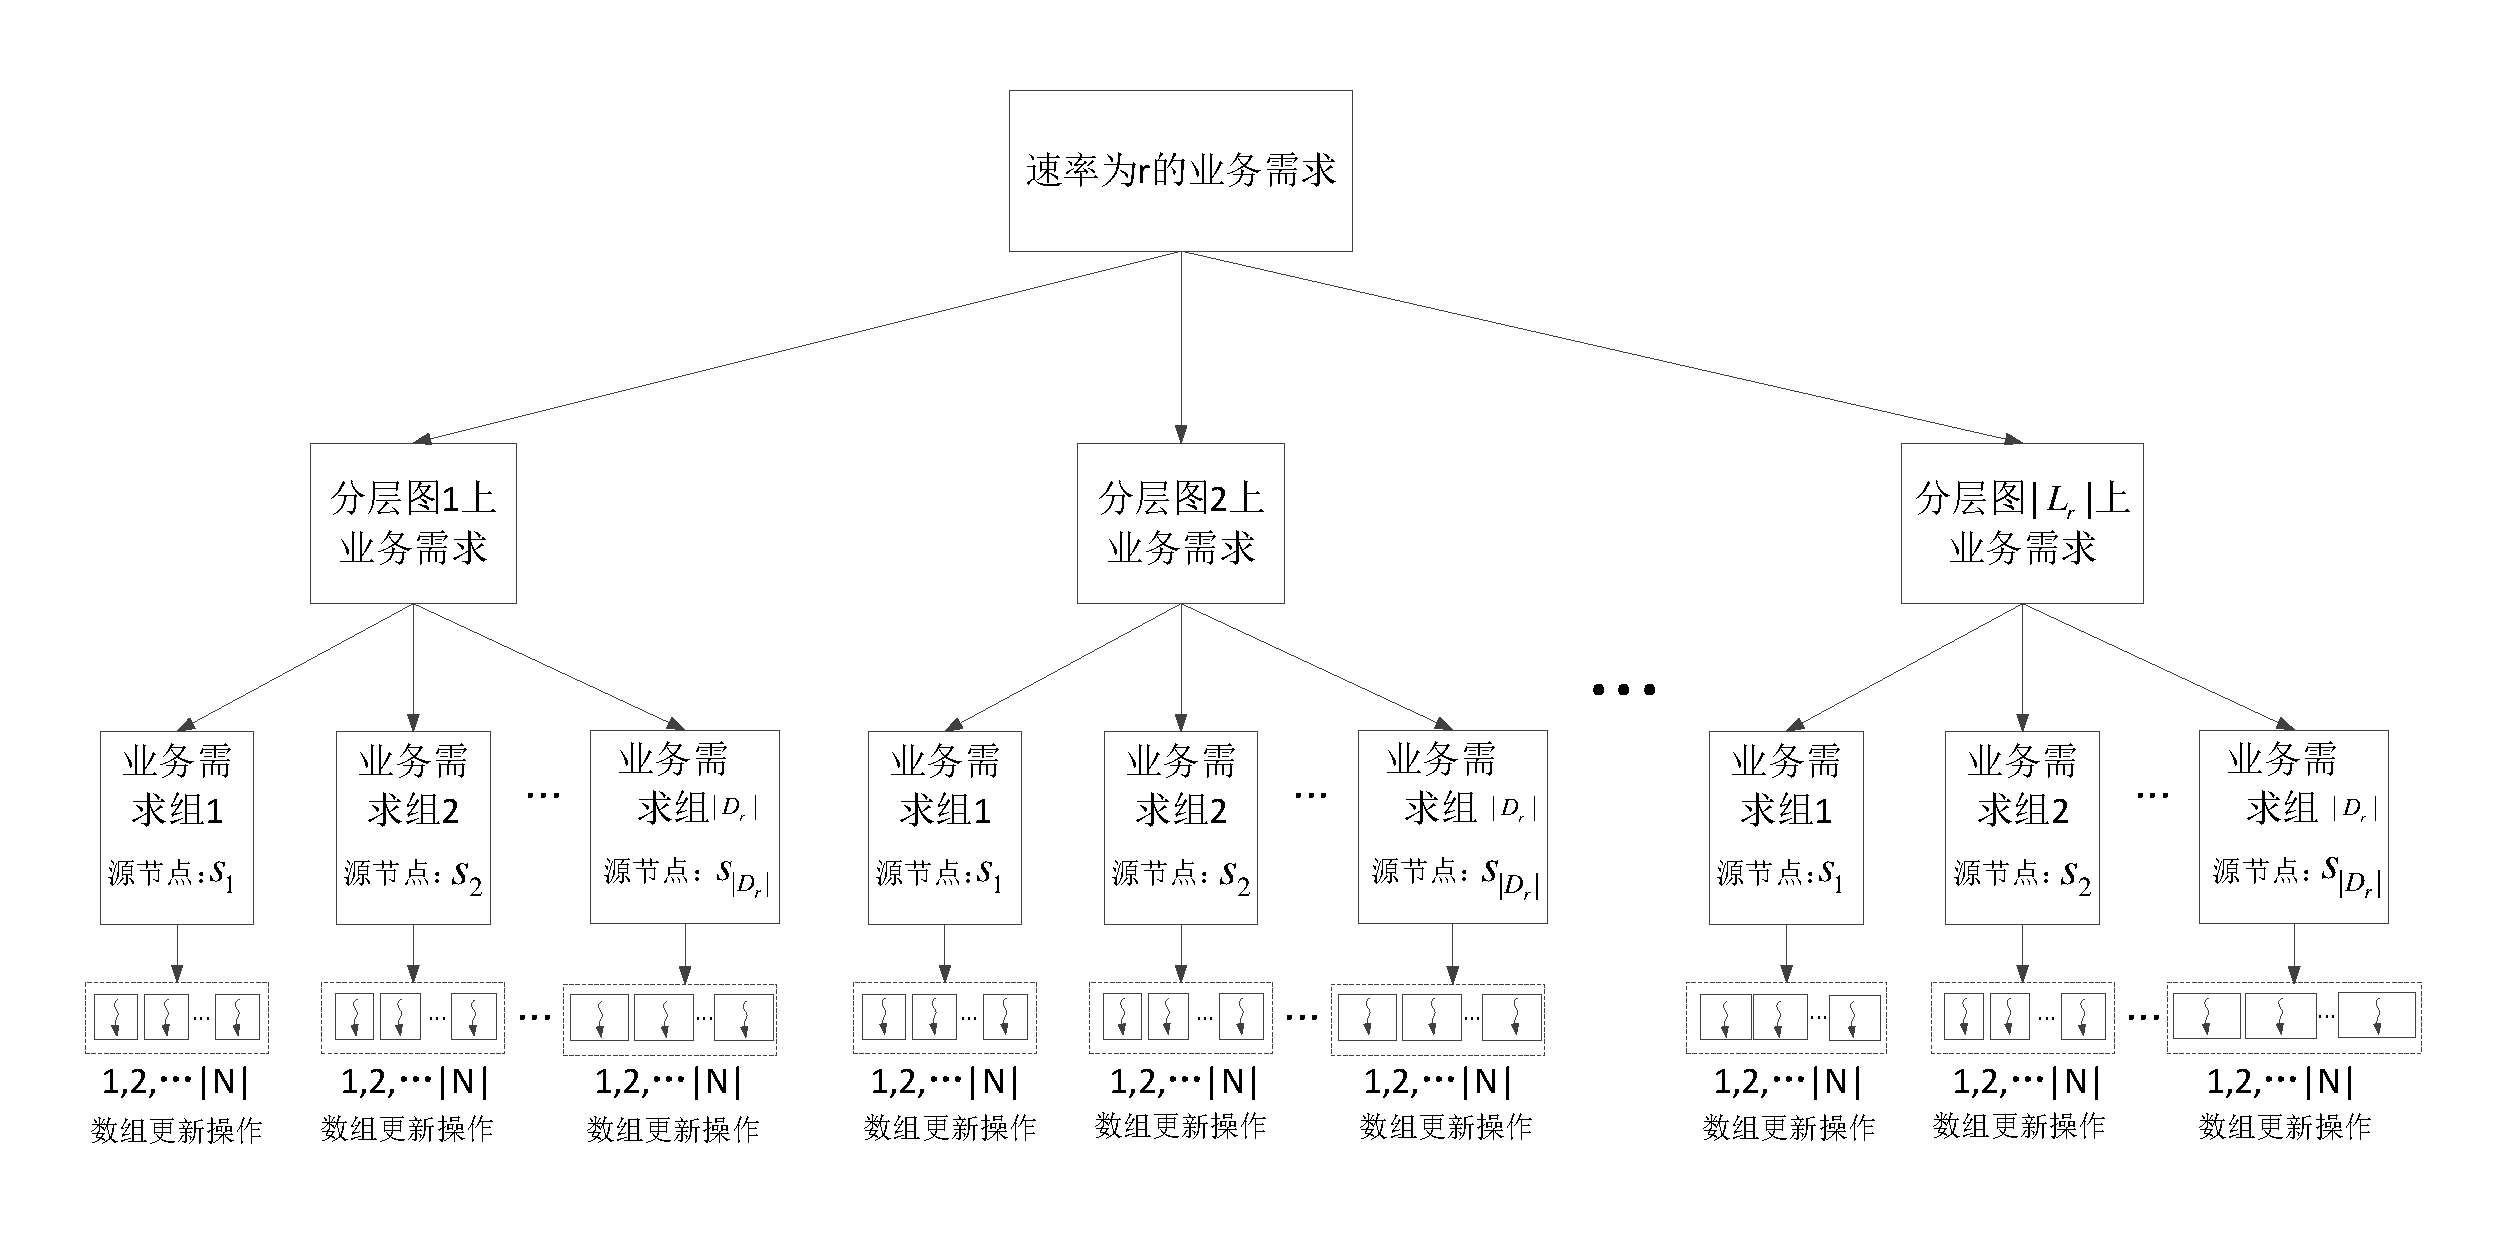
\includegraphics[width=1 \textwidth]{figures/DRK.pdf}}
\end{center}
\caption{{\footnotesize{同速率业务的动态规划并行示意图}}}
\label{dbs}
\end{figure*}
\subsection{不同速率间业务的并行}
和BFS一样,对不同速率的业务,本文依然采用不同的流进行并行,其并行过程如图\ref{BBK}所示。
\begin{figure*}
\setlength{\abovecaptionskip}{-0.5cm}
%\setlength{\belowcaptionskip}{-0.5cm}
\begin{center}
{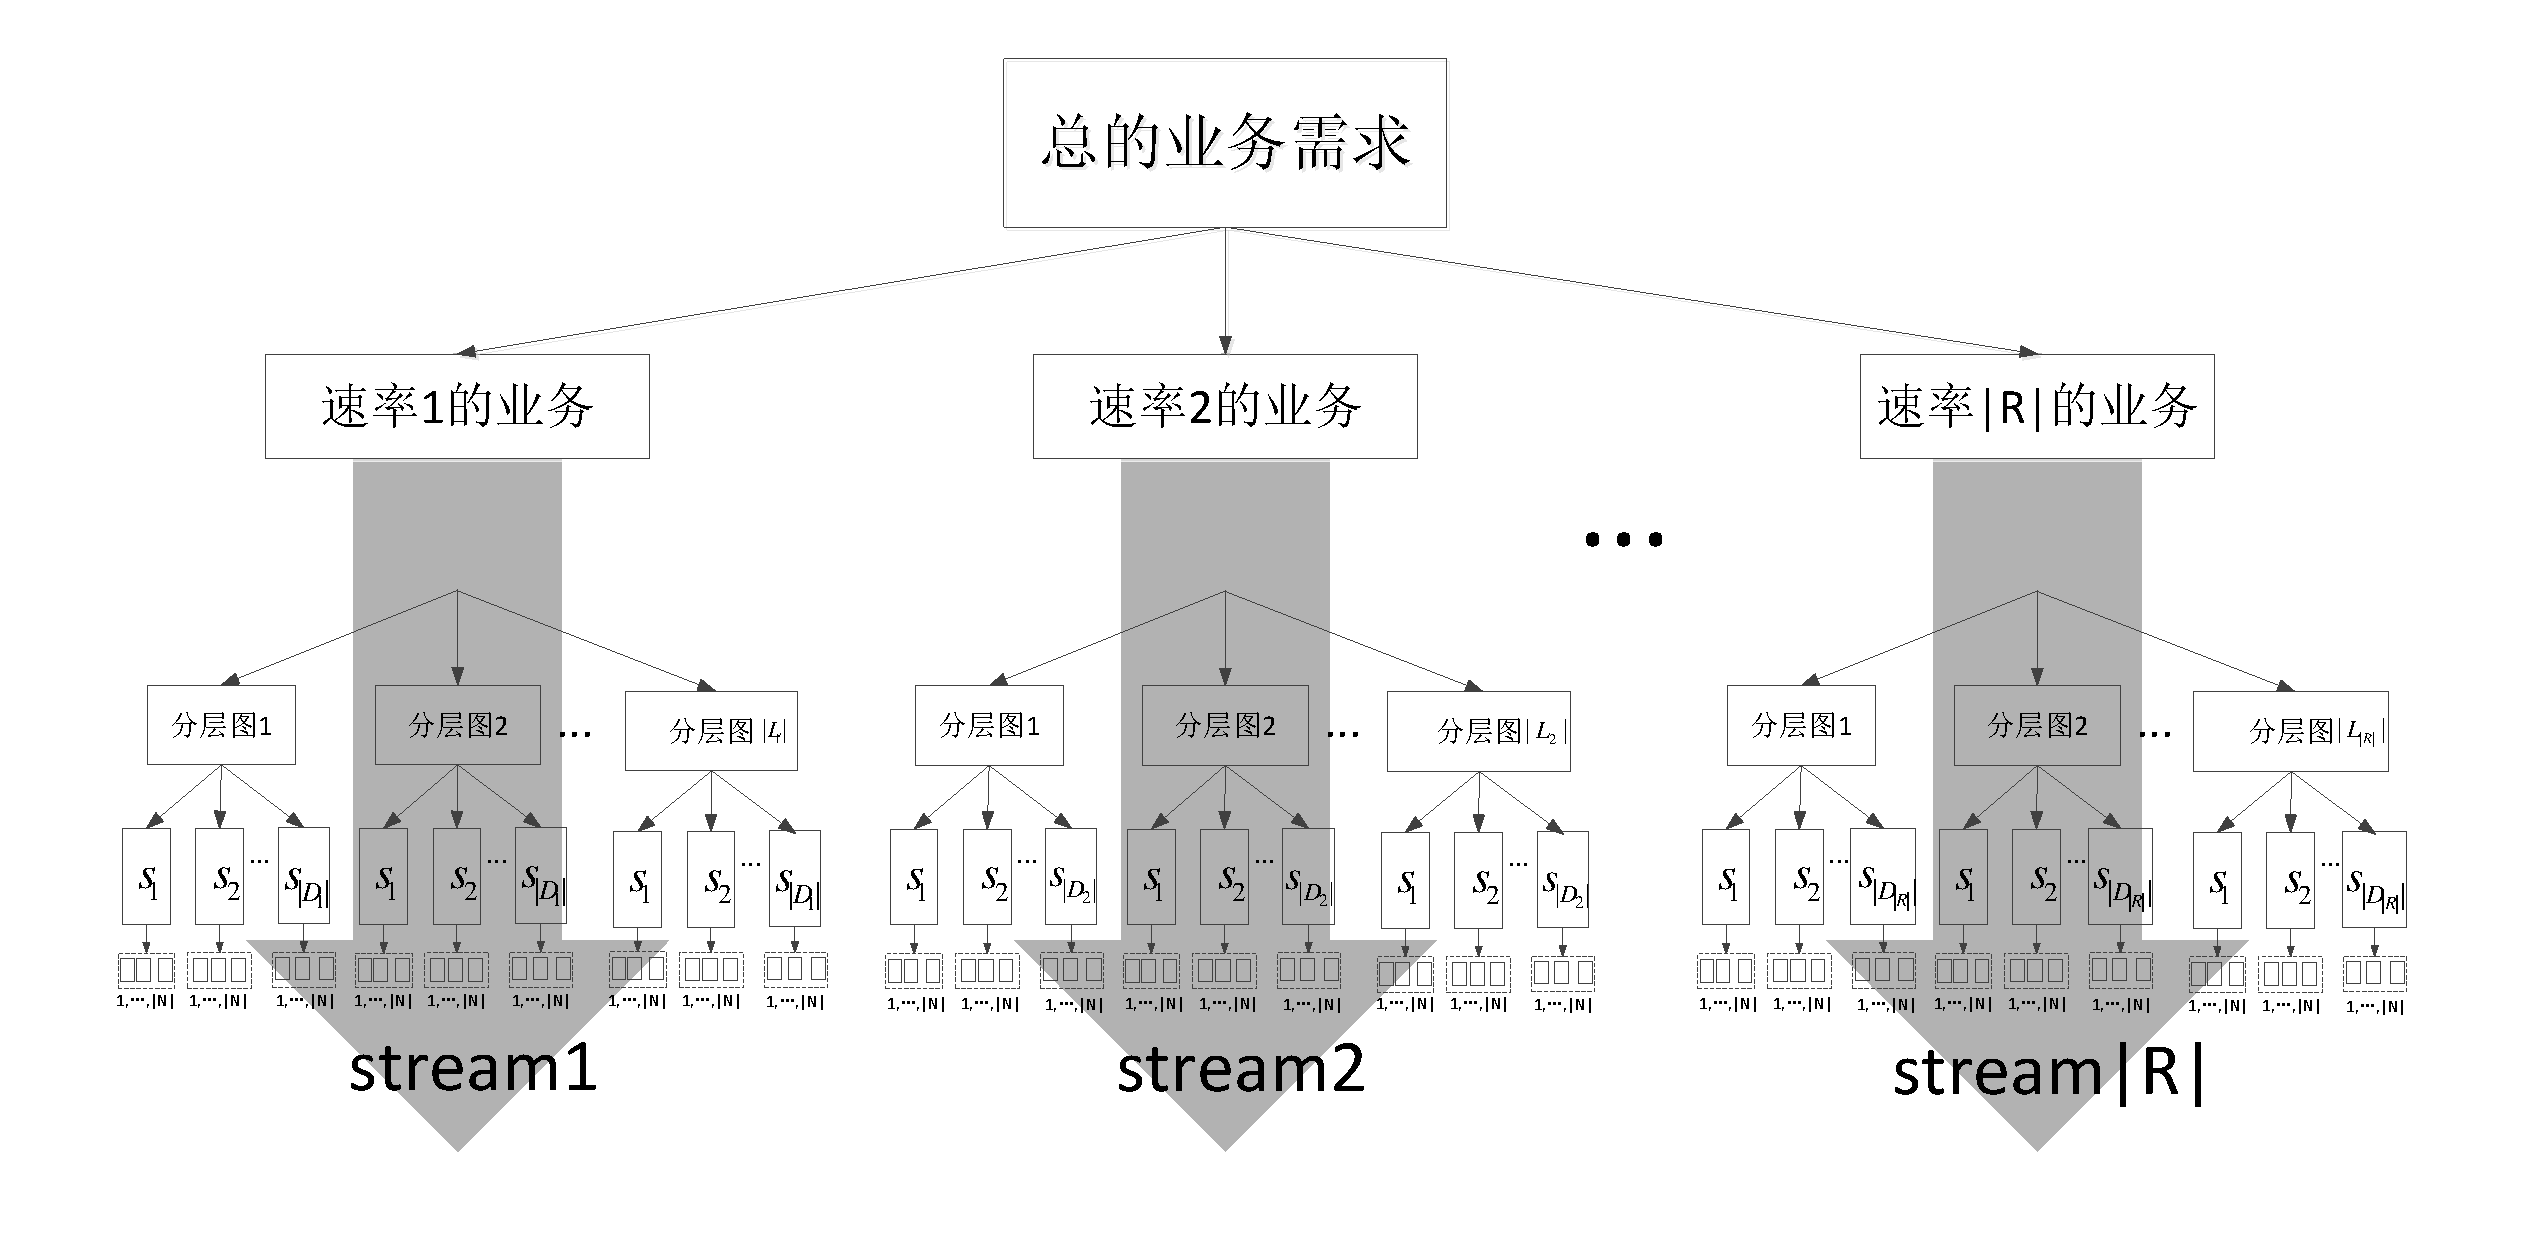
\includegraphics[width=1 \textwidth]{figures/BBK.pdf}}
\end{center}
\caption{{\footnotesize{动态规划流并行示意图}}}
\label{BBK}
\end{figure*}
\subsection{GPU上的kernel设计}
\begin{algorithm}[t]
\begin{algorithmic}[1]
\Function{kernel\_dynamic\_update}{$PE$,$rid$,$k$}
\State {$bid \leftarrow$ block ID}
\State {$tid \leftarrow$ thread ID}
\State {将$(bid,tid,rid)$ 映射到边的标号$nid$}
\State {将$(bid,tid,rid)$ 映射到源节点的标号$sid$}
\State {将$(bid,tid,rid)$ 映射到分层图标号$lid$}
\For {$e \in PE[lid][nid]$}
\If{链路$e$没有被占用}
\If {$Price[lid][sid][nid][k]<Price[lid][sid][e.tail][k-1]+e.weight$}
\State{$Price[lid][sid][nid][k]=Price[lid][sid][e.tail][k-1]+e.weight$}
\State{$Pre[lid][sid][nid][k]=e.tail$}
\EndIf
\EndIf
\EndFor
\EndFunction
\end{algorithmic}
\caption{kernel\_dynamic\_update}
\label{KernelDynamic}
\end{algorithm}

动态规划的并行算法中我们只需要一个kernel($kernel\_dynamic\_update$),如算法\ref{KernelDynamic}所示,在kernel中,输入$PE$是一个二维的集合数组,比如,$PE[2][3]$表示第2个分层图上点3的入边集合。$Price$ 是预先分配的代价数组,他是一个四维数组,第一维表示当前代价数组对应的分层图标号,第二维度表示源节点,第三维度表示目的节点,第四维度表示路径的跳数,比如$Price[4][3][10][5]$=7 表示在第4个分层图上,点3到点10的跳数为5的最优路径代价为7,初始时,当跳数等于0 时,除了源节点代价被初始化为0之外,其他的距离都被初始化为无穷大。$Pre$数组是前驱数组用以记录前驱信息来恢复路径,$Pre$数组和$Price$数组一样,是一个四维数组,$Pre[4][3][10][5]$=50表示在第4个分层图上,点3到点10的跳数为5的最优路径的前驱节点(也就是路径上的倒数第二个点)为点50。$rid$表示当前kernel 负责计算的业务速率标号,他是区分不同流的标记,$rid$ 不同表示执行kernel的流不同。$k$ 表示当前扩展的层数,也就是跳数。算法开始时先进行一系列映射操作,将线程映射到点标号$eid$,当前所在分层图标号$lid$,以及源节点标号$sid$。映射完成后就可以进行$Price$数组的更新了,也就是要去寻找最优的入边,算法遍历点的所有入边。由于动态情况下,边的可用状态可能发生变化,找到边之后,需要判断这条边是否可用,如果不可用则跳过这条边,反之,就判断更新条件是否成立($Price[lid][sid][nid][k]<Price[lid][sid][e.s][k-1]+e.weight$),如果条件成立则说明这条入边比之前的要好,经过这条边到达当前点的路径代价更小,所以要更新$Price$数组,同时为了后面恢复路径,需要记录前驱信息在数组$Pre$中。

算法\ref{Parad}展示了整个动态规划的计算过程,算法开始时先将业务按照速率的不同进行划分,再将业务按照源节点的不同划分成不同的业务组集合,比如,$D_r \in D$表示速率为$r$ 的业务组集合,$d_{rs} \in D_r$ 表示速率为$r$的源节点标号为$s$的业务组。划分好业务组之后,就开始初始化代价数组,将速率对应的所有分层图上的跳数为0的源节点代价初始化为0,这是一个三层的for循环,第一层遍历速率标号,第二层遍历源节点标号,第三层遍历速率所对应的分层图标号。初始化$Price$数组后,在发射kernel之前需要先新建$|R|$ 个GPU 流,不同的流将对不同速率的业务进行计算。$k$为扩展的跳数标记,开始时$k$初始化为1。while循环中进行扩展操作,其中$W_{max}$为跳数限制,最大跳数不能超过$W_{max}$,所以最多只能循环$W_{max}$次。while循环中for循环用来发射不同的流,因为发射不同流的kernel 是异步操作,for循环不会去等待上一个kernel结束了才去执行下一个kernel,所以可以认为所有kernel都是同时发射的。
\begin{algorithm}[t]
\begin{algorithmic}[1]
\Require
业务需求集合$D$;
各个分层图前驱链路集合$PE$;
\Ensure {业务需求的最短路径集合$P$}
\State {将业务根据速率和源节点重新组合成业务分组集合$D$}
\For {$D_r \in D$}
\For {$d_{rs} \in D_r$}
\For {$l \in L_r$}
\For {$v \in V$}
\If {$v==s$}
\State {$Price[l][s][v][0]\leftarrow$ 0}
\Else
\State {$Price[l][s][v][0]\leftarrow \infty $}
\EndIf
\EndFor
\EndFor
\EndFor
\EndFor
\State {新建$|R|$个流,组成集合$S$}
\State {$k \leftarrow$ 1}
\While{$k<=W_{max}$}
\For{$r \in R$}
\State {在流$S_r$上发射 kernel\_dynamic\_update($PE$,$rid$,$k$)}
\EndFor
\State{$k=k+1$}
\EndWhile
\State {根据前驱数组$Pre$重建路径,然后把路径加入到集合$P$}
\end{algorithmic}
\caption{{并行动态规划的计算}}
\label{Parad}
\end{algorithm}


\section{实验仿真分析}
\subsection{对比算法}
为了说明TESAA对路径代价和网络阻塞率带来的优化效果,我们将PTESAA/STESAA和不进行路由代价优化的贪心算法进行比较,我们称这个算法为GRSAA(Greedy Routing and Spectrum Allocation Algorithm),如算法\ref{ParaSPC}所示。当业务到达时,GRSAA先在第一层对所有业务求最短路径,为每个业务估计一个路由代价,按照这个路由代价对业务进行升序排序,这是为了优先加入较短的业务。然后,算法逐层去寻找是否能够把业务加入到当前层中,如果能加入到当前层中,那么就更新当前层上的相应链路的占用情况,反之,就在下一层进行搜寻。如果所有层都无法加入这个业务,那么业务就被阻塞,业务被加入到阻塞集合。
\begin{algorithm}[t]
\begin{algorithmic}[1]
\Require
业务需求集合$D$;
分层图集合$G$;
\Ensure {业务需求的路径集合$P$;阻塞的需求集合$Z$}
\For{$r \in R$}
\State{$flag \leftarrow 0$ }
\For{$D_r \in D$}
\State{把$D_r$中的业务按照其在第一层分层图上的最短路径值进行升序排序}
\For{$d \in D_r$}
\For{$g \in G_r$}
\If{在分层图$g$上存在业务$d$的合法路径$p$}
\State{更新分层图$g$上的链路占用情况}
\State{把路径$p$加入到结果路径集合$P$中}
\State{$flag \leftarrow 1$}
\State{\bfseries break}
\EndIf
\EndFor
\If{$flag=0$}
\State{把业务$d$加入阻塞集合$Z$中}
\EndIf
\EndFor
\EndFor
\EndFor
\end{algorithmic}
\caption{{贪心的分层RSA算法}}
\label{ParaSPC}
\end{algorithm}
\subsection{实验设置}
在本文的实验仿真中,网络的节点数为$N=100$,平均度数为$4$,业务的路径限制$W_{max}=8$。我们假设只存在两种速率的业务,并且已知两种速率的业务的大致比例为1:3。我们初始时为速率1的业务分配20层的频谱连续分层网络,为速率2的业务分配60层的频谱连续的分层网络。我们假设业务的到达服从泊松过程,一共产生了1000个到达事件,每两个连续的到达事件之间的时间间隔服从均值为4的负指数分布,当到达事件发生时,实验产生速率1的业务为$d_1$ 个,产生速率为2的业务$d_2$ 个,其中$d1$ 为$2 \cdot |N|$到$4 \cdot|N|$中的随机值,$d_2$为$6 \cdot |N|$到$12 \cdot |N|$之间的随机值。假设每个业务的服务时间满足均值为$ST$的负指数分布,我们观察各种算法在不同平均服务时间$ST$下的优化情况。

在本文的实验仿真中,网络实时发生变化,每次业务到达时的网络情况都有很大不同,所以数据的变化幅度较大,另外,我们产生了1000次加入事件,加入事件较多,横坐标较窄,这样不利于观察数据的变化趋势。为了方便作图,我们对实验数据进行平滑操作,我们采用取平均值的方法对数据进行平滑操作,我们设置一个窗口值$S=10$,假设数据的横坐标为$x$,数据值为$f(x)$,那么平滑后的数据值$f' \left( x \right)$为$\frac{\sum\limits_{p \in (x-S/2,x+S/2)}{f(p)}}{S-1}$。本章中关于时间,路由代价,和路由跳数的仿真实验图都做过平滑操作,只有阻塞率变化图没有做平滑操作。

\subsection{无权图下的仿真结果}
\subsubsection{路由跳数优化结果分析}

在无权图中,TESAA的优化目标是最小化路由的跳数,图\ref{B5H}到图\ref{B40H}展示了无权图下跳数的优化结果,我们把PTESAA和STESAA与贪心算法GRSAA进行比较。图中的横坐标表示业务到达的次数,图中的纵坐标表示业务的平均路由跳数。

当网络状况较好的时候,比如图\ref{B5H}中,平均服务时间为$ST=5$时,PTESAA/STESAA计算得到的路由平均跳数为2.73,而GRSAA计算得到的路由平均跳数为3.73,PTESAA/STESAA得到的路由平均跳数要比GRSAA得到的路由平均跳数少一跳左右。随着平均服务时间$ST$的增加,PTESAA/STESAA和GRSAA所计算出的路由平均跳数都有所增加,但是PTESAA/STESAA的增幅较小,从$ST=5$时的平均2.73增加到$ST=40$时的平均2.82,而GRSAA的平均路由跳数随着$ST$的增加而大幅增加,从$ST=5$ 时的平均3.75增加到$ST=40$时的平均4.2,可见不管在网络空闲还是网络繁忙的情况下PTESAA都能很好地优化业务路由的跳数,减小对网络资源的占用。
\begin{figure*}
\setlength{\abovecaptionskip}{-0.5cm}
%\setlength{\belowcaptionskip}{-1cm}
\begin{center}
{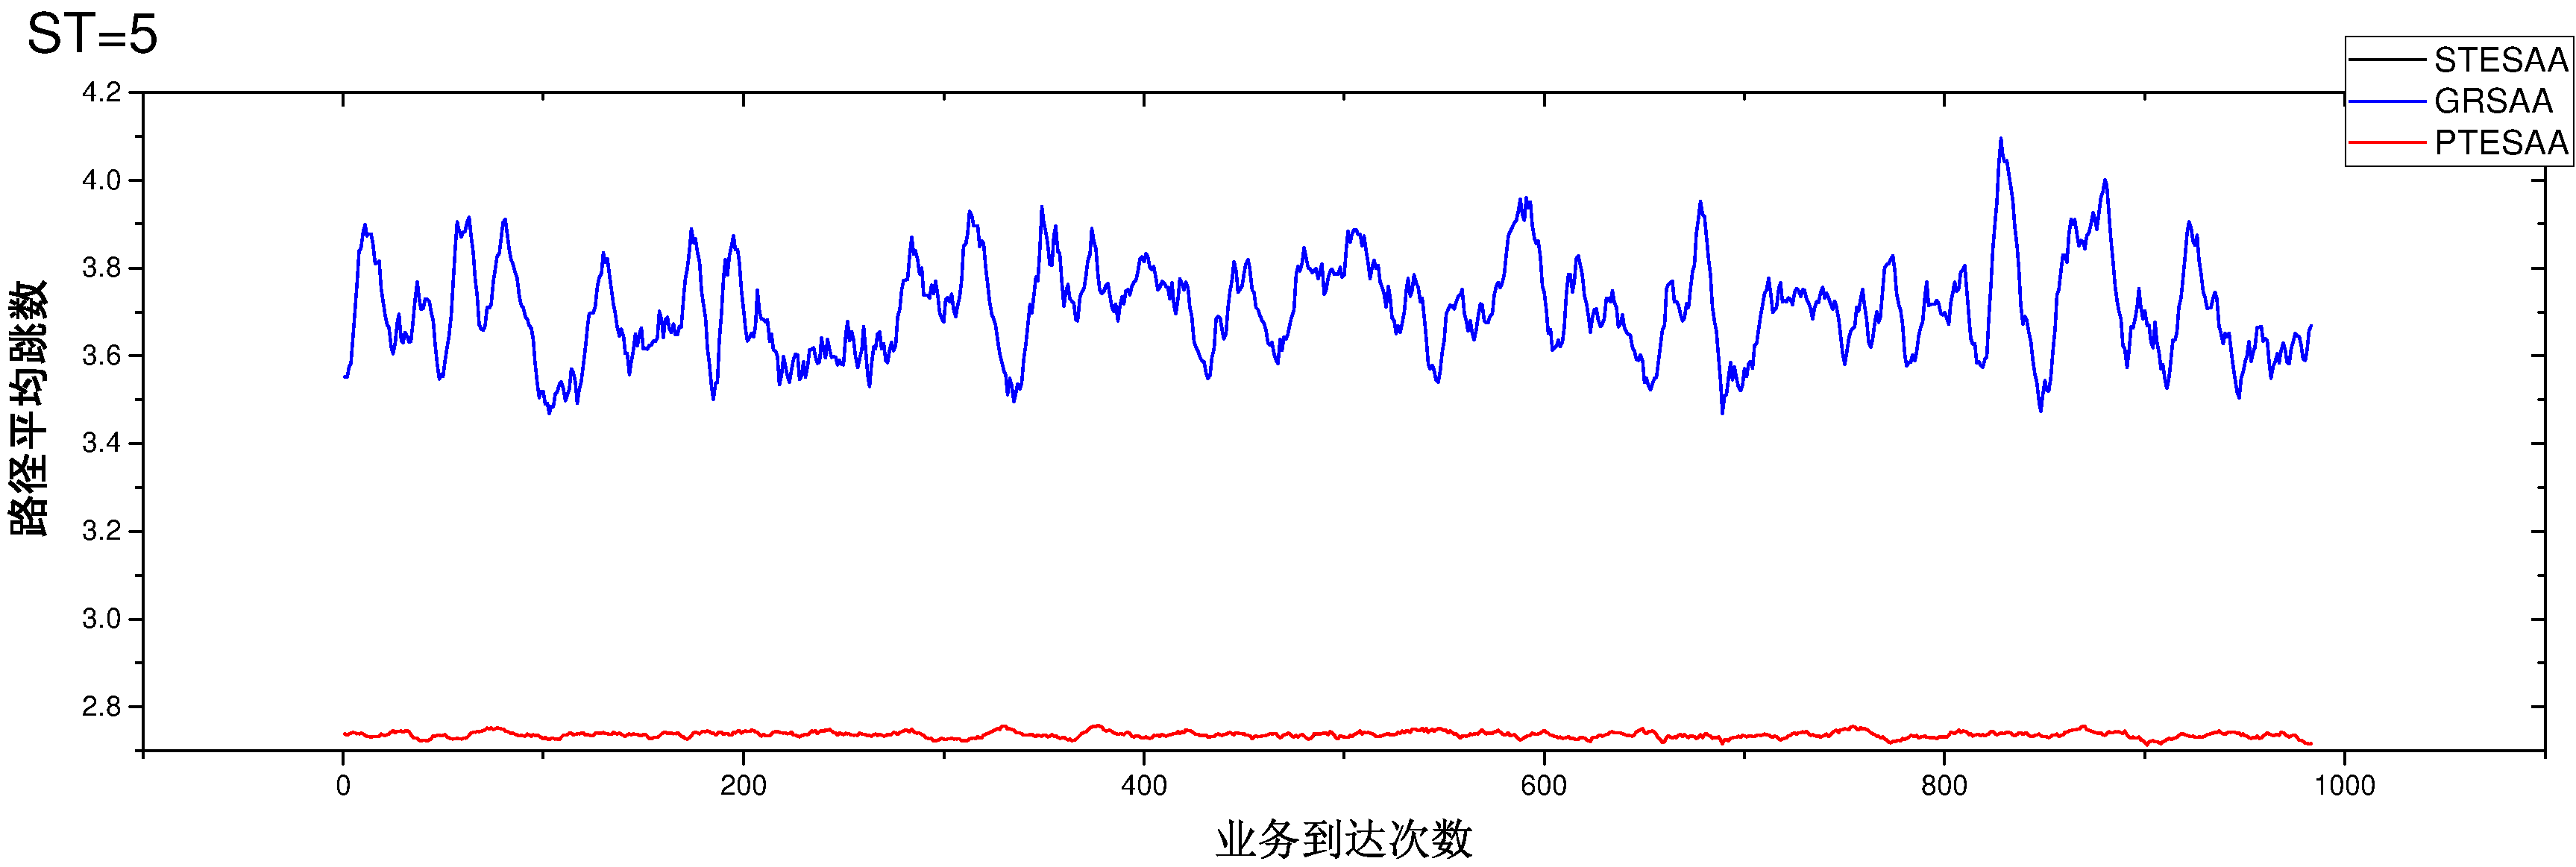
\includegraphics[width=1 \textwidth]{figures/B5H.pdf}}
\end{center}
\caption{{\footnotesize{无权图路径跳数对比(ST=5)}}}
\label{B5H}
\end{figure*}
\begin{figure*}
\vspace{-0.5cm}
\setlength{\abovecaptionskip}{-0.5cm}
%\setlength{\belowcaptionskip}{-1cm}
\begin{center}
{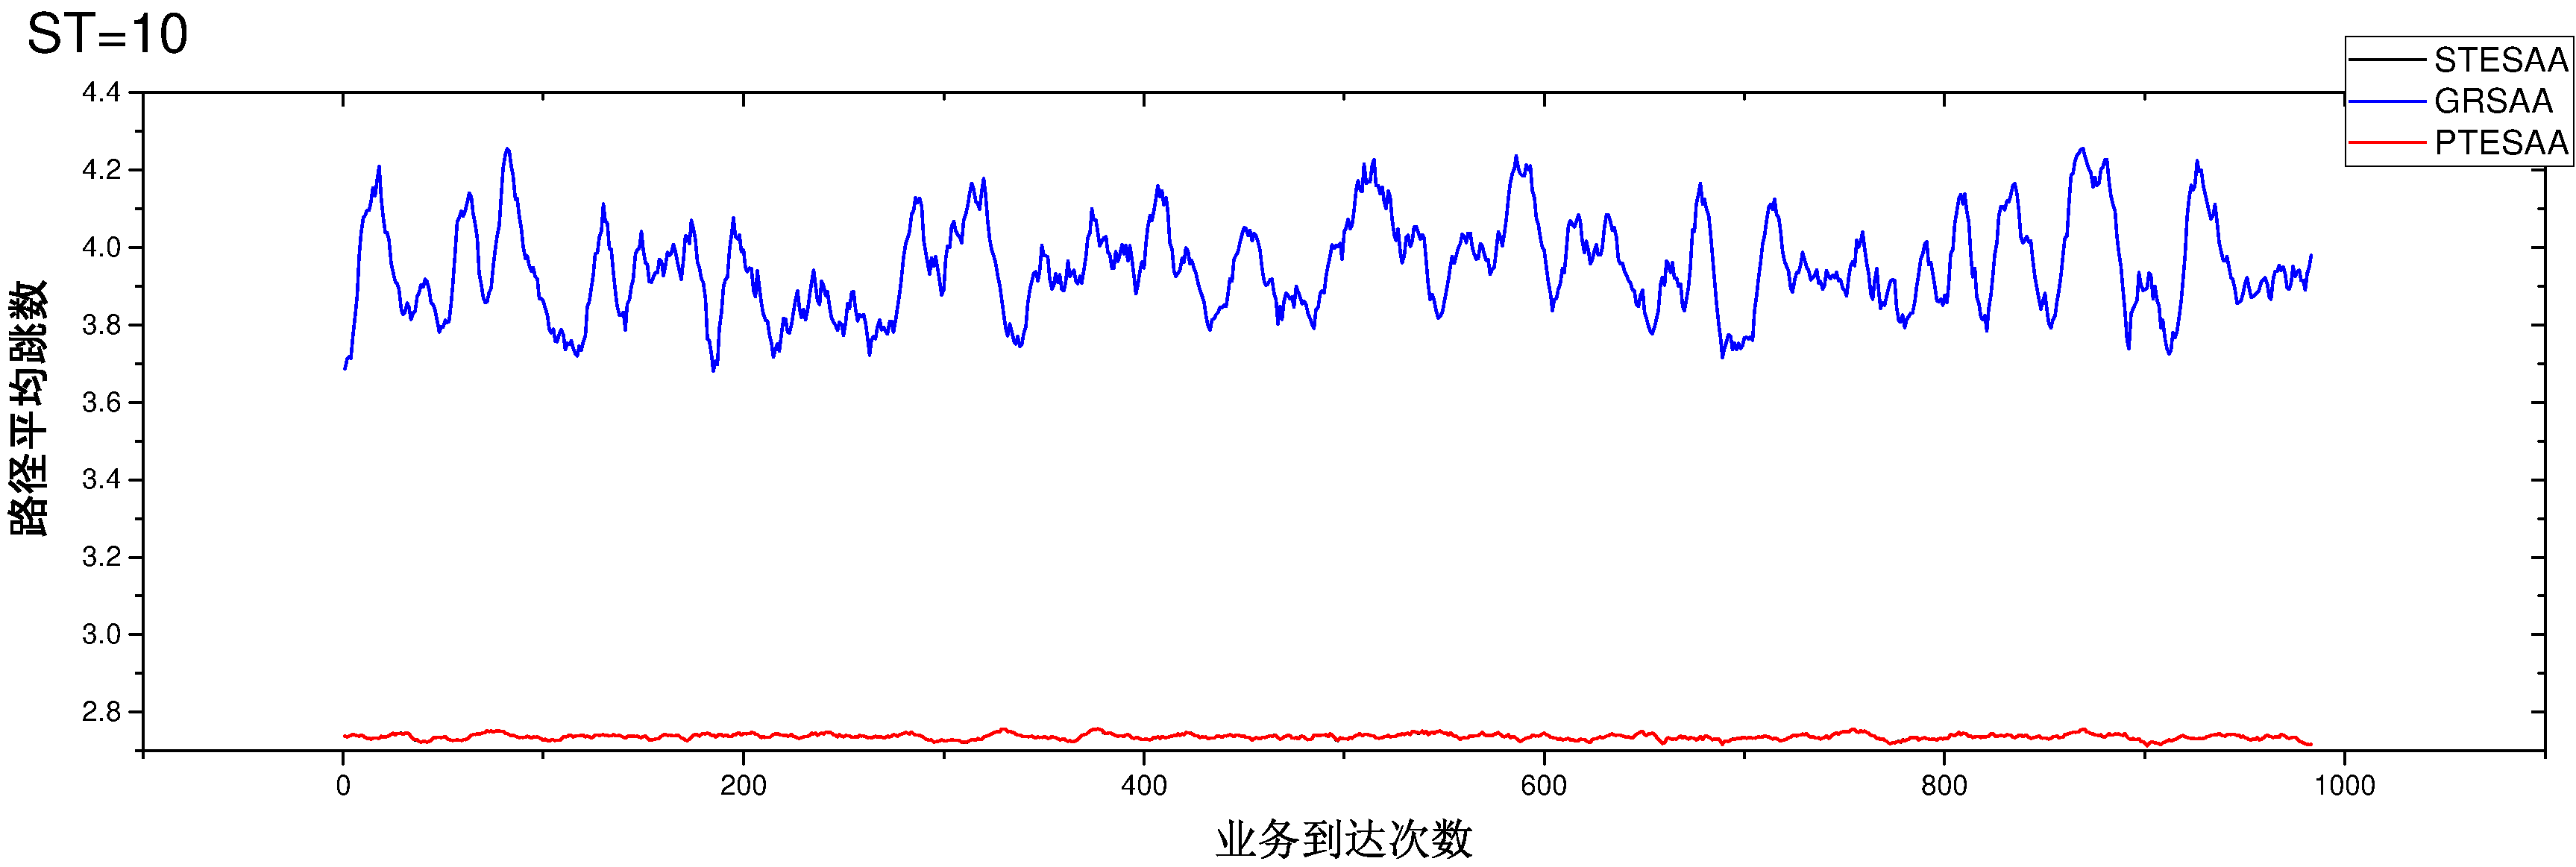
\includegraphics[width=1 \textwidth]{figures/B10H.pdf}}
\end{center}
\caption{{\footnotesize{无权图路径跳数对比(ST=10)}}}
\label{B10H}
\end{figure*}
\begin{figure*}
\vspace{-0.5cm}
\setlength{\abovecaptionskip}{-0.5cm}
%\setlength{\belowcaptionskip}{-1cm}
\begin{center}
{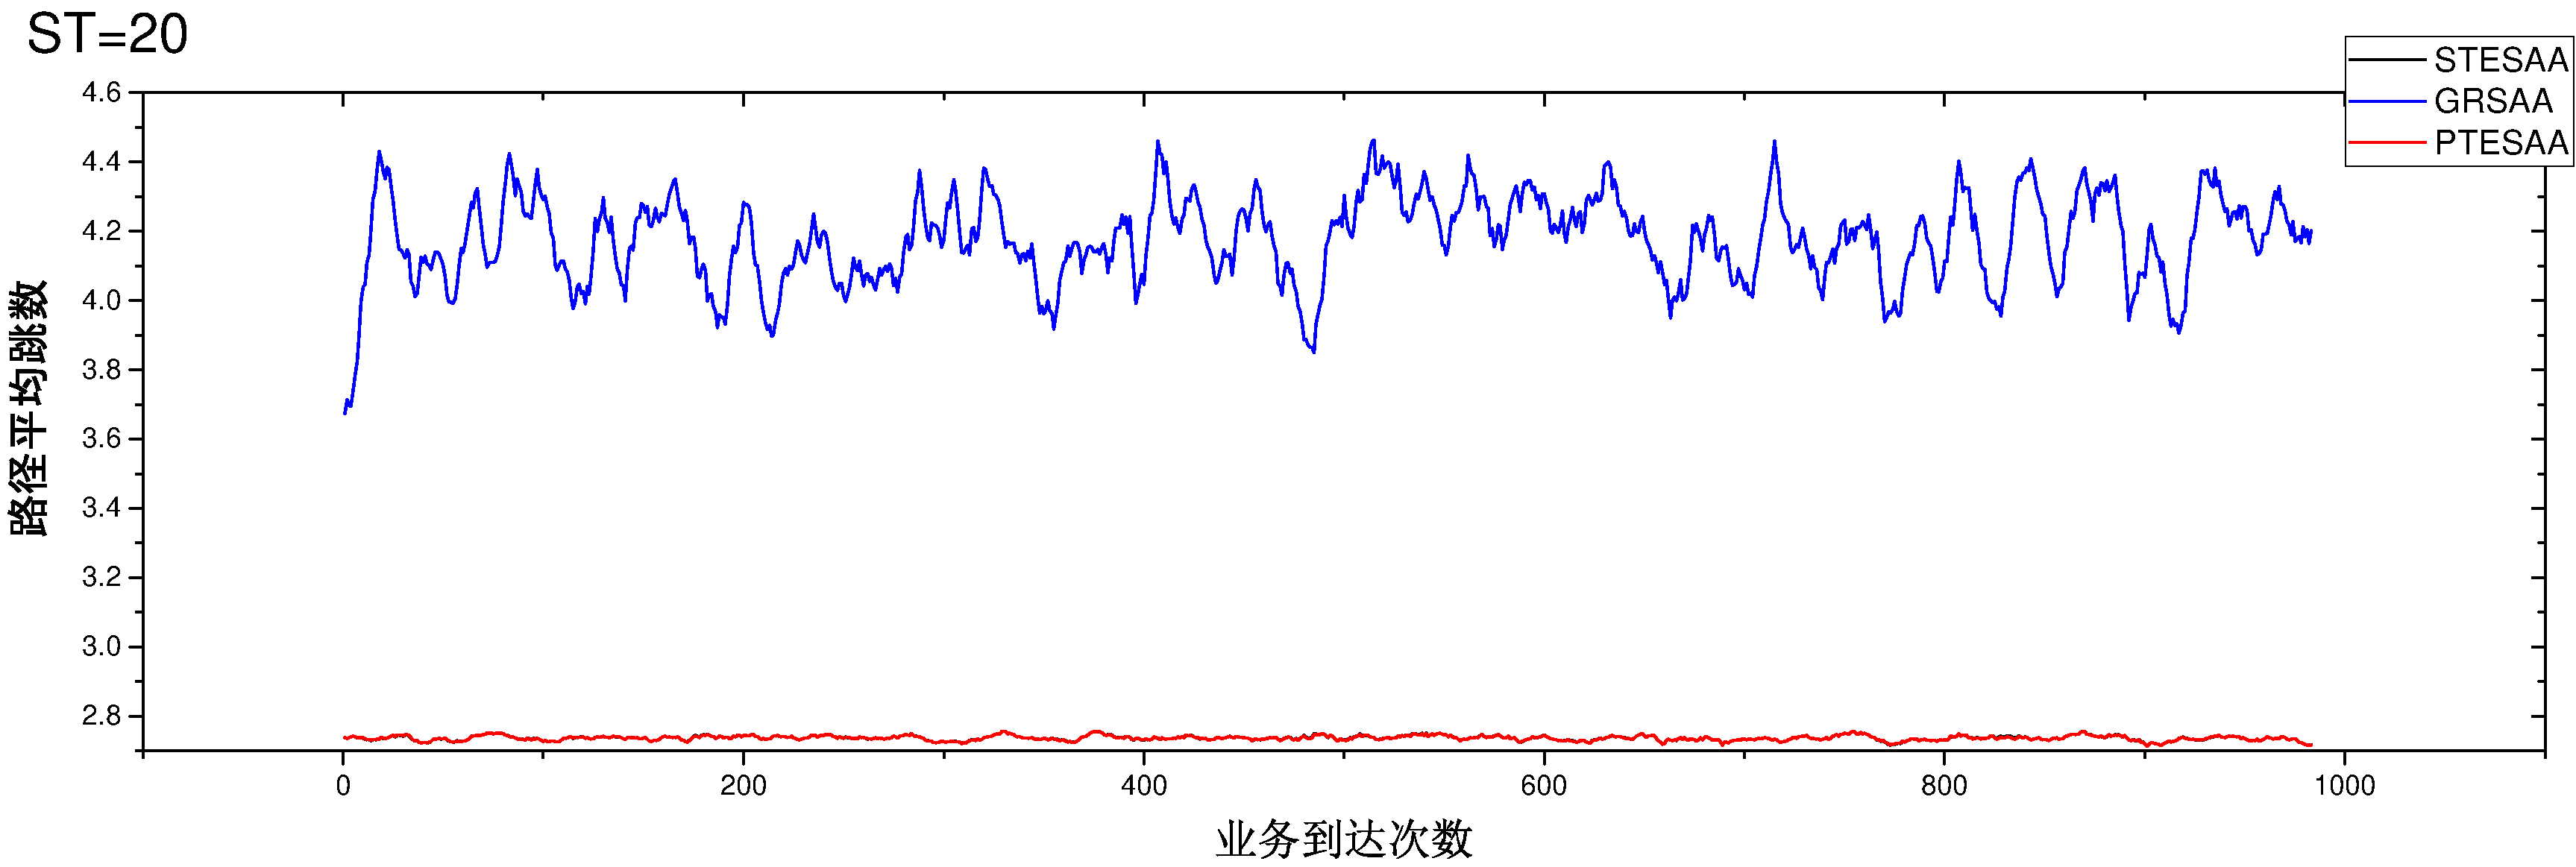
\includegraphics[width=1 \textwidth]{figures/B20H.pdf}}
\end{center}
\caption{{\footnotesize{无权图路径跳数对比(ST=20)}}}
\label{B20H}
\end{figure*}
\begin{figure*}
\vspace{-0.5cm}
\setlength{\abovecaptionskip}{-0.5cm}
%\setlength{\belowcaptionskip}{-1cm}
\begin{center}
{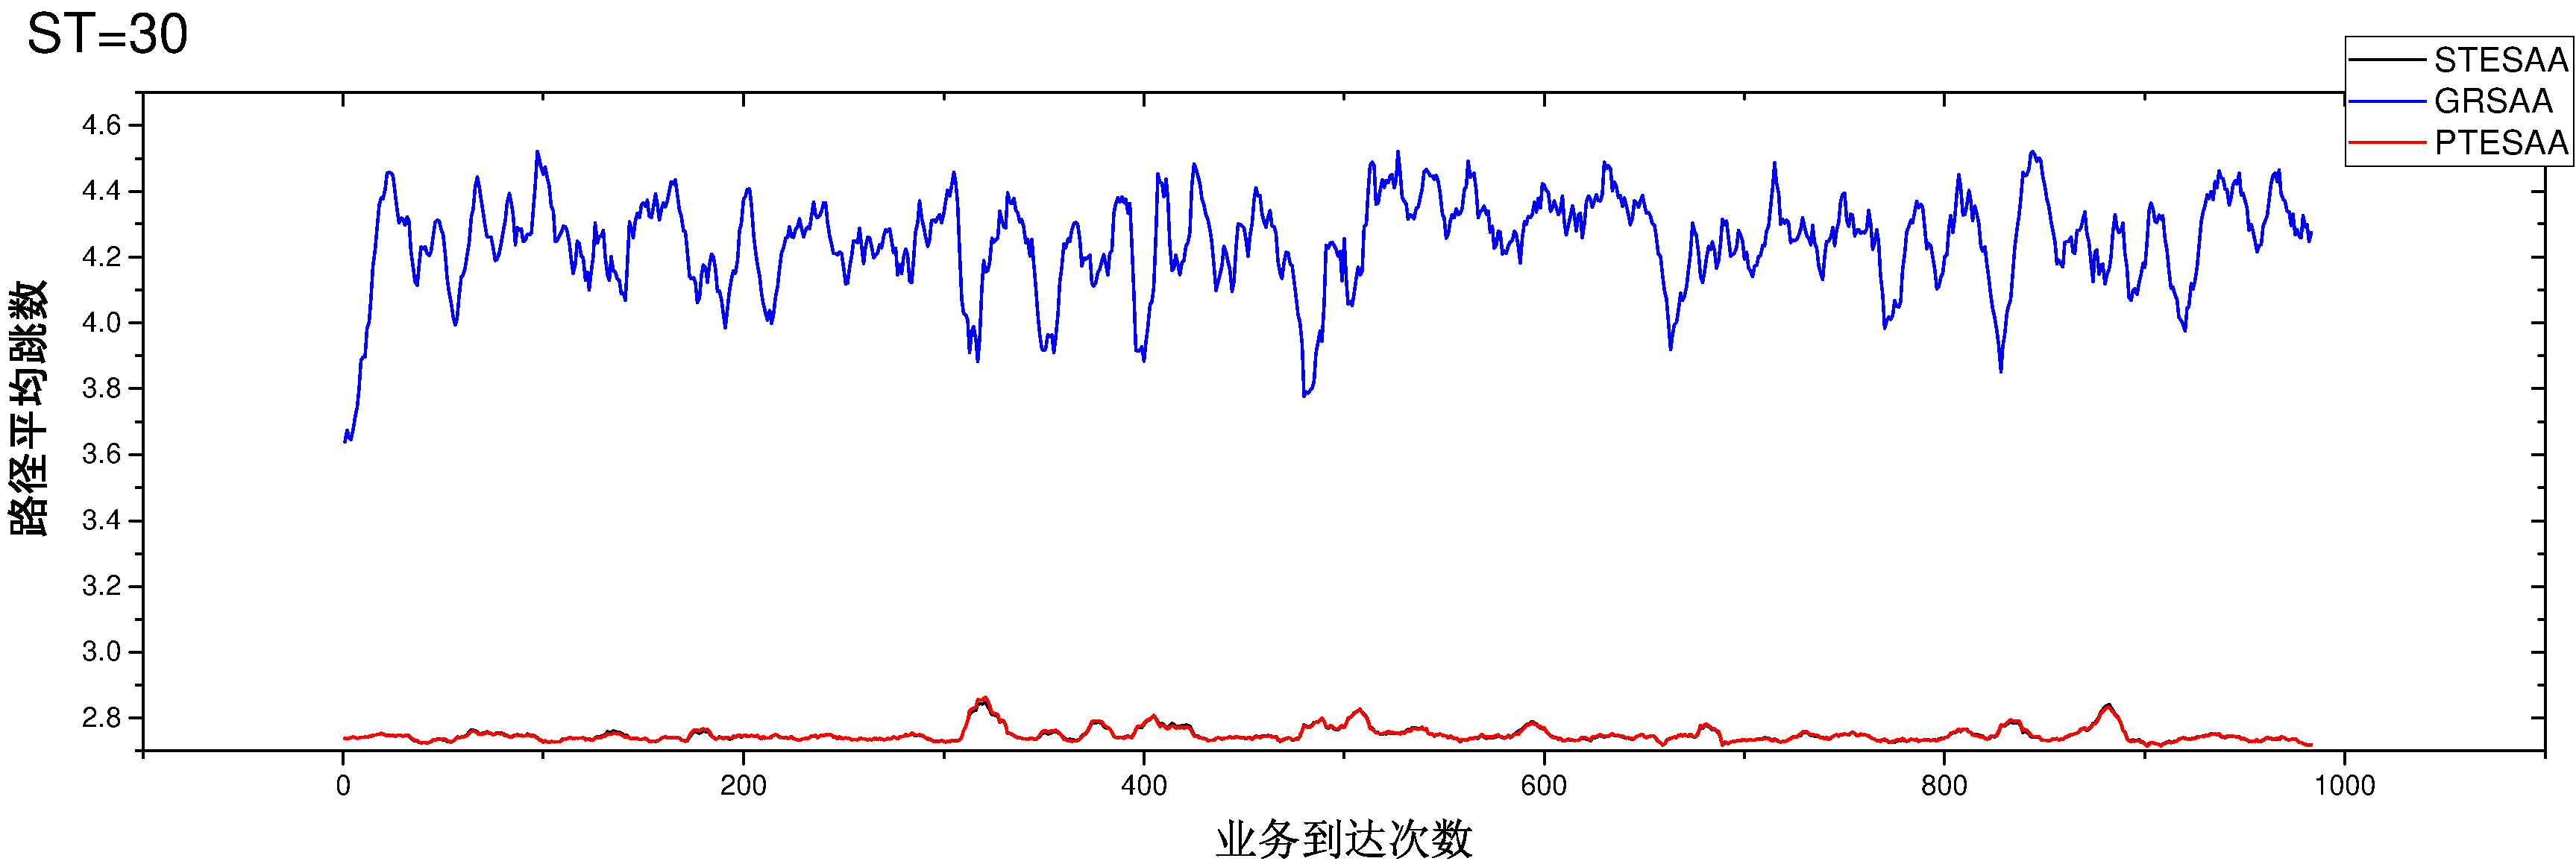
\includegraphics[width=1 \textwidth]{figures/B30H.pdf}}
\end{center}
\caption{{\footnotesize{无权图路径跳数对比(ST=30)}}}
\label{B20H}
\end{figure*}
\begin{figure*}
\vspace{-0.5cm}
\setlength{\abovecaptionskip}{-0.5cm}
%\setlength{\belowcaptionskip}{-1cm}
\begin{center}
{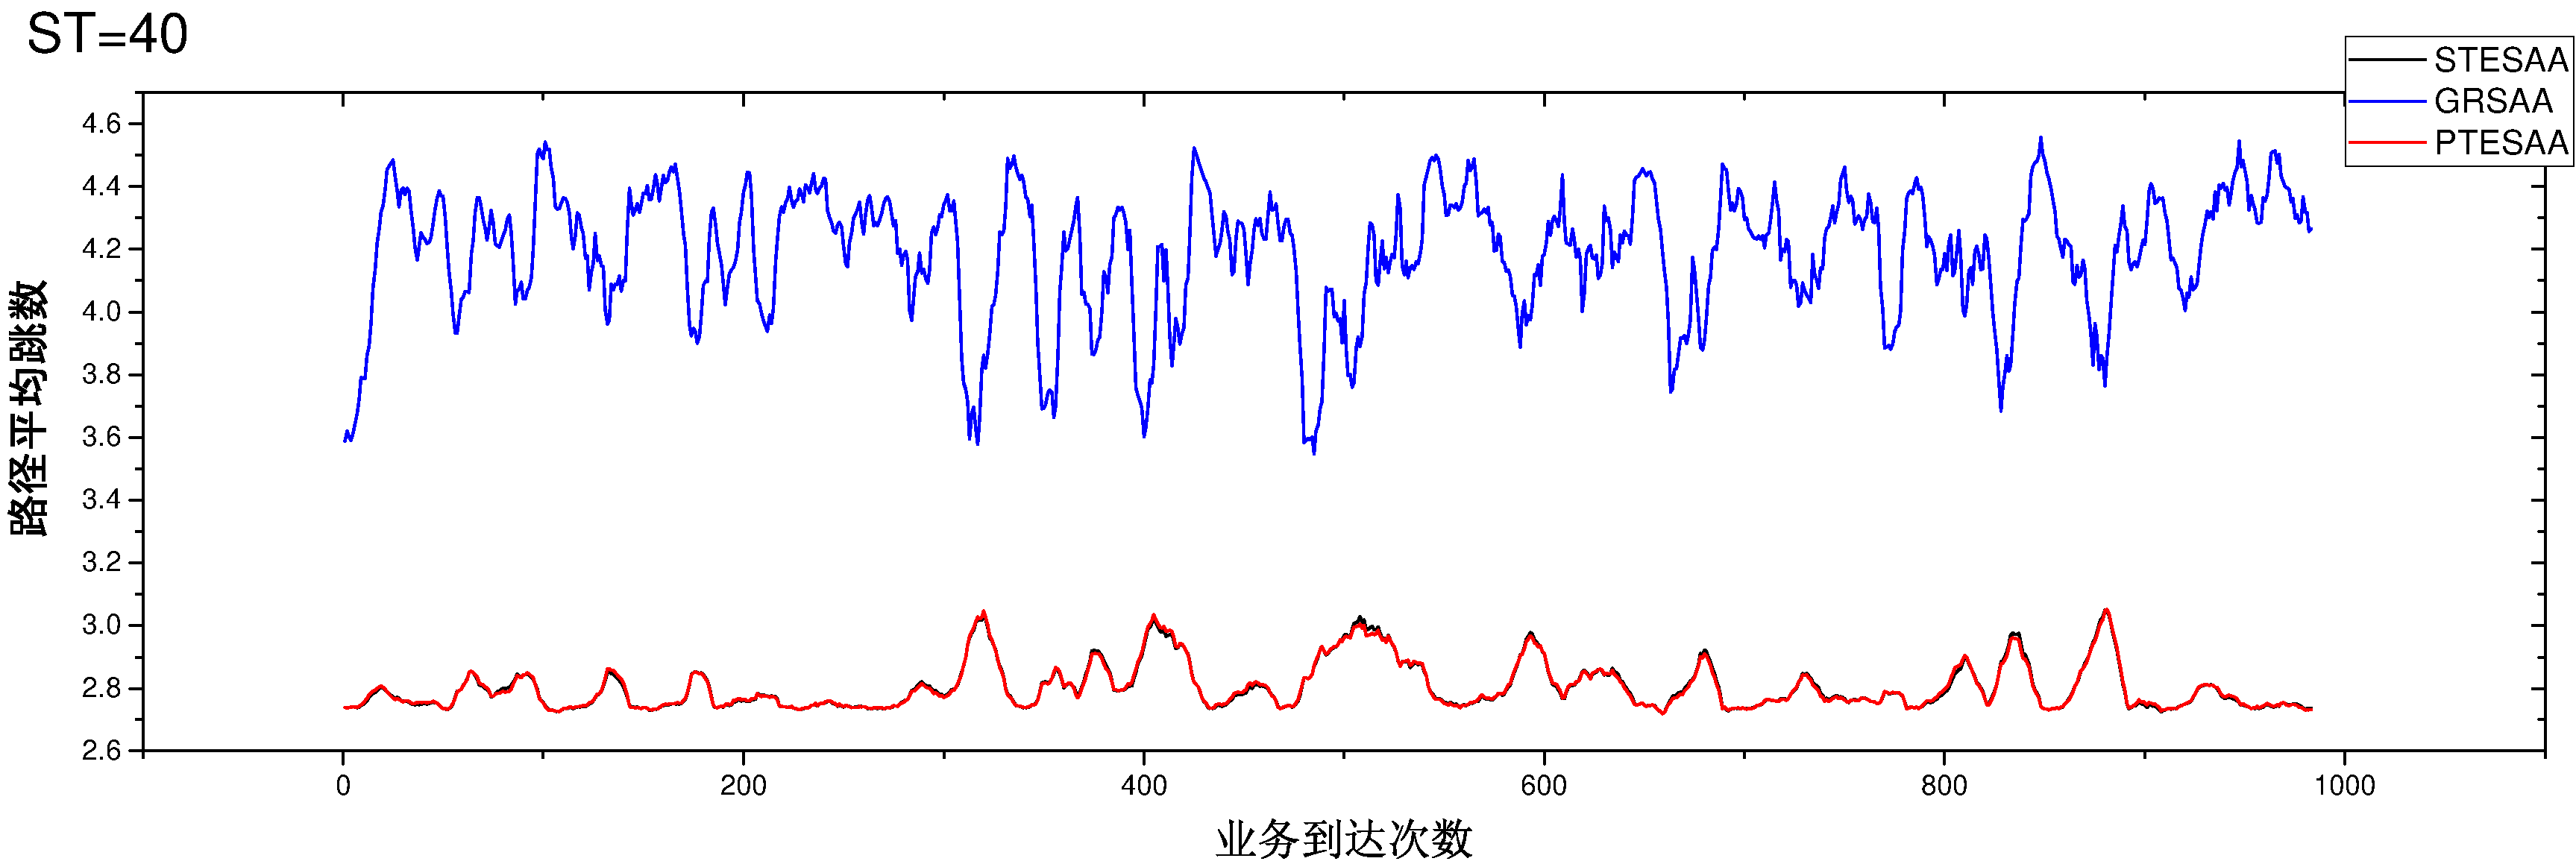
\includegraphics[width=1 \textwidth]{figures/B40H.pdf}}
\end{center}
\caption{{\footnotesize{无权图路径跳数对比(ST=40)}}}
\label{B40H}
\end{figure*}
\subsubsection{时间分析}

图 \ref{B5T}到图 \ref{B40T}展示了各个算法在不同平均服务时间$ST$下的计算时间,当$ST=5$时,我们可以看到通过GPU加速的PTESAA的计算时间是STESAA计算时间的1/4,而实际上,步骤一的GPU加速比可达7-8倍,但是由于步骤二的快速路由选择算法所占用的时间也不可忽略,而我们没有对这部分算法进行GPU加速,这使得总体的加速比下降为4-5倍。

图\ref{B5T}到图\ref{B40T}显示GRSAA的计算时间略高于PTESAA的计算时间,可见PTESAA不仅可以优化路由跳数,而且在时间上也比GRSAA更有优势。

观察图\ref{B5T}到图\ref{B40T},我们发现随着$ST$的变化,PTESAA对STESAA的加速比略有下降,这是因为随着网络压力的增加,可用链路变少,使得STESAA中步骤一的计算量下降,PTESAA的加速优势变小。
\subsubsection{阻塞率分析}
图 \ref{B10Z}到图 \ref{B40Z}展示了随着$ST$的增加,PTESAA/STESAA和GRSAA算法的阻塞率变化情况。其中PTESAA,STESAA由于是同一种算法,所以其阻塞率几乎一样。当$ST=10$时,我们发现PTESAA/STESAA的阻塞次数明显小于GRSAA。 当$ST=20$时,PTESAA/STESAA的阻塞次数和阻塞幅度均小于GRSAA,在GRSAA中出现了一次相对较大的阻塞,但是PTESAA/STESAA中没有出现这种不平稳的阻塞率突变。当$ST=30$时,我们发现PTESAA/STESAA的阻塞次数和阻塞幅度比GRSAA小很多,GRSAA的平均阻塞率是PTESAA/STESAA的6倍左右。当$ST=40$时,PTESAA,STESAA和GRSAA的阻塞率都增加很多,但是PTESAA/STESAA的阻塞情况还是大大优于GRSAA,可见在网络拥塞的情况下,PTESAA/STESAA依然能够有效地减小阻塞率。
\begin{figure*}
\vspace{-0.5cm}
\setlength{\abovecaptionskip}{-0.5cm}
%\setlength{\belowcaptionskip}{-0.1cm}
\begin{center}
{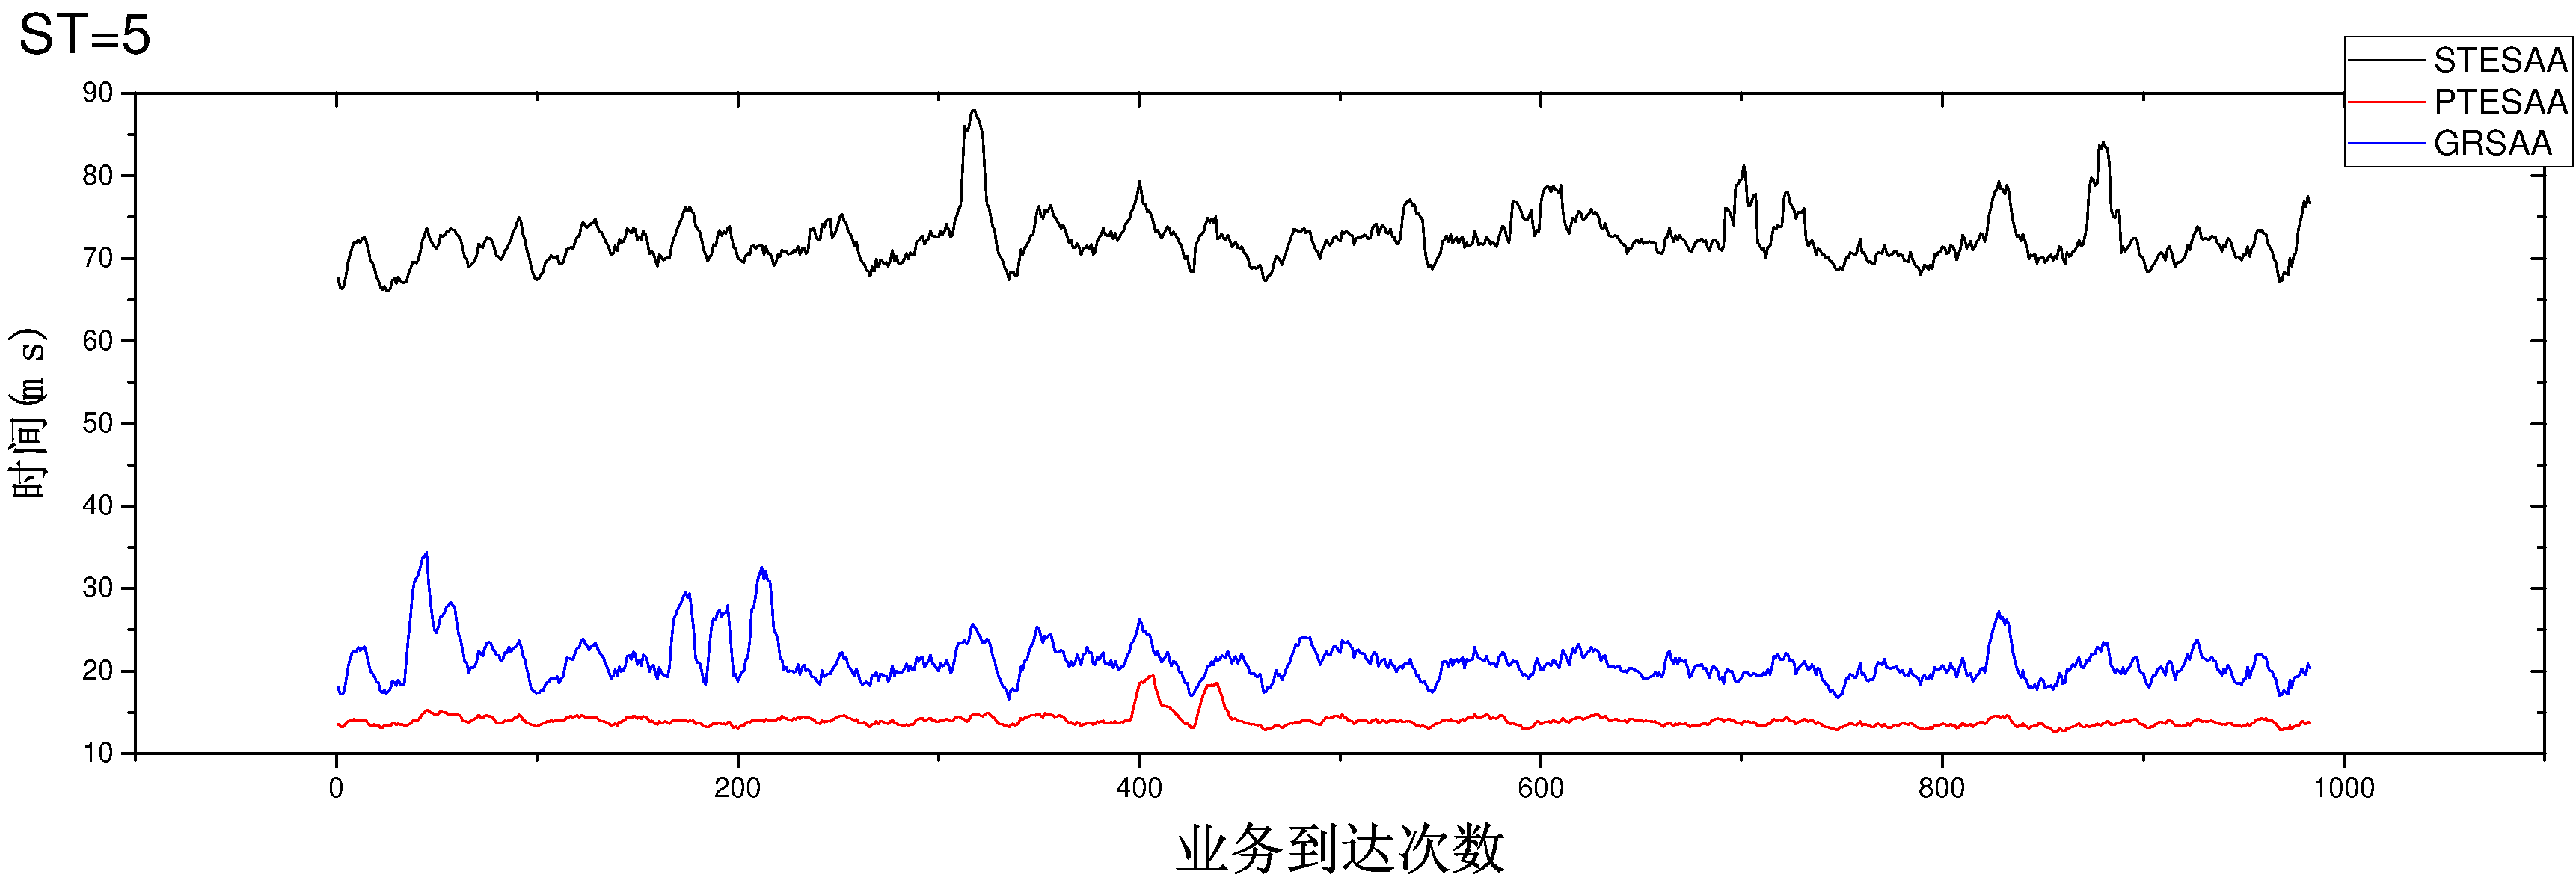
\includegraphics[width=1 \textwidth]{figures/B5T.pdf}}
\end{center}
\caption{{\footnotesize{无权图时间对比(ST=5)}}}
\label{B5T}
\end{figure*}
\begin{figure*}
\vspace{-0.5cm}
\setlength{\abovecaptionskip}{-0.5cm}
%\setlength{\belowcaptionskip}{-0.5cm}
\begin{center}
{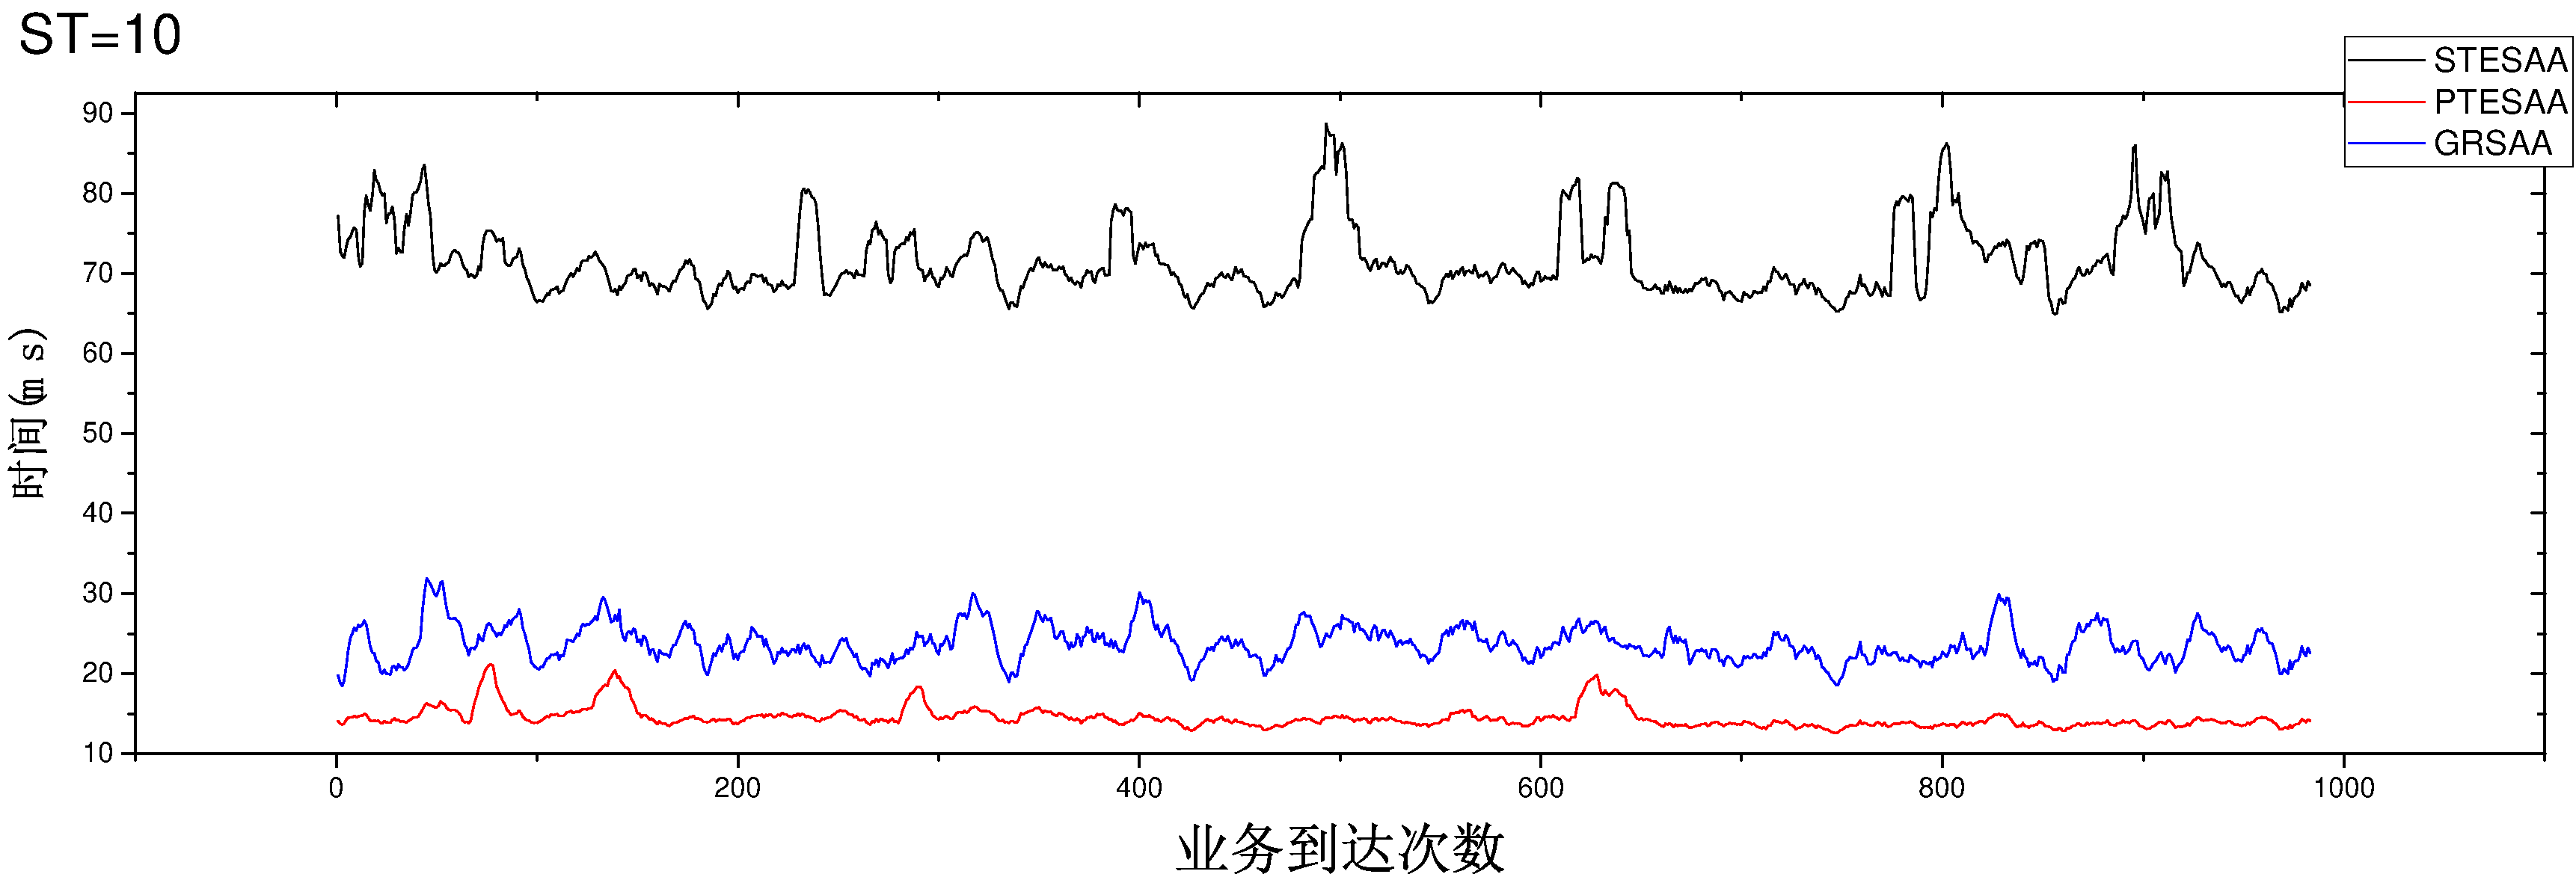
\includegraphics[width=1 \textwidth]{figures/B10T.pdf}}
\end{center}
\caption{{\footnotesize{无权图时间对比(ST=10)}}}
\label{B10T}
\end{figure*}
\begin{figure*}
\vspace{-0.5cm}
\setlength{\abovecaptionskip}{-0.5cm}
\begin{center}
{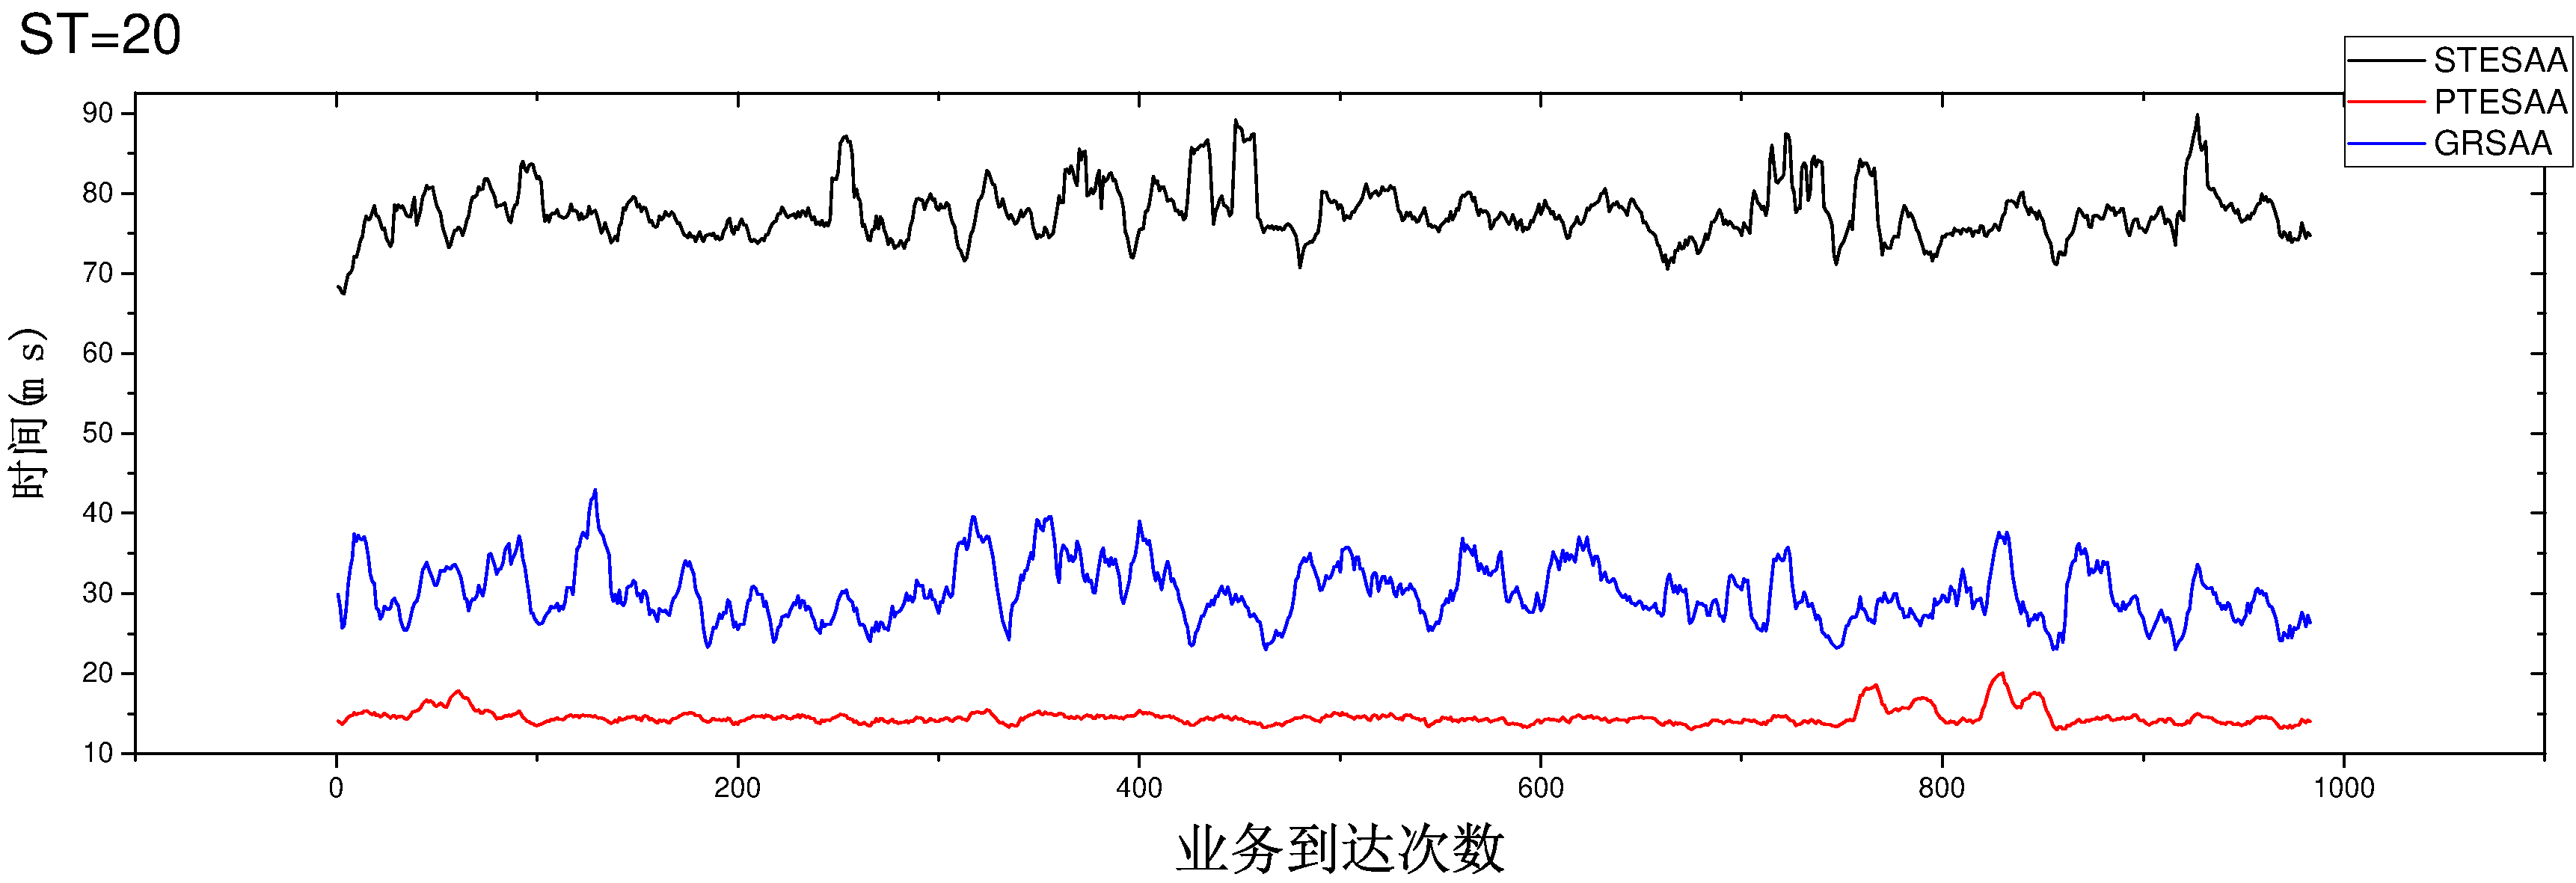
\includegraphics[width=1 \textwidth]{figures/B20T.pdf}}
\end{center}
\caption{{\footnotesize{无权图时间对比(ST=20)}}}
\label{B20T}
\end{figure*}
\begin{figure*}
\vspace{-0.5cm}
\setlength{\abovecaptionskip}{-0.5cm}
\begin{center}
{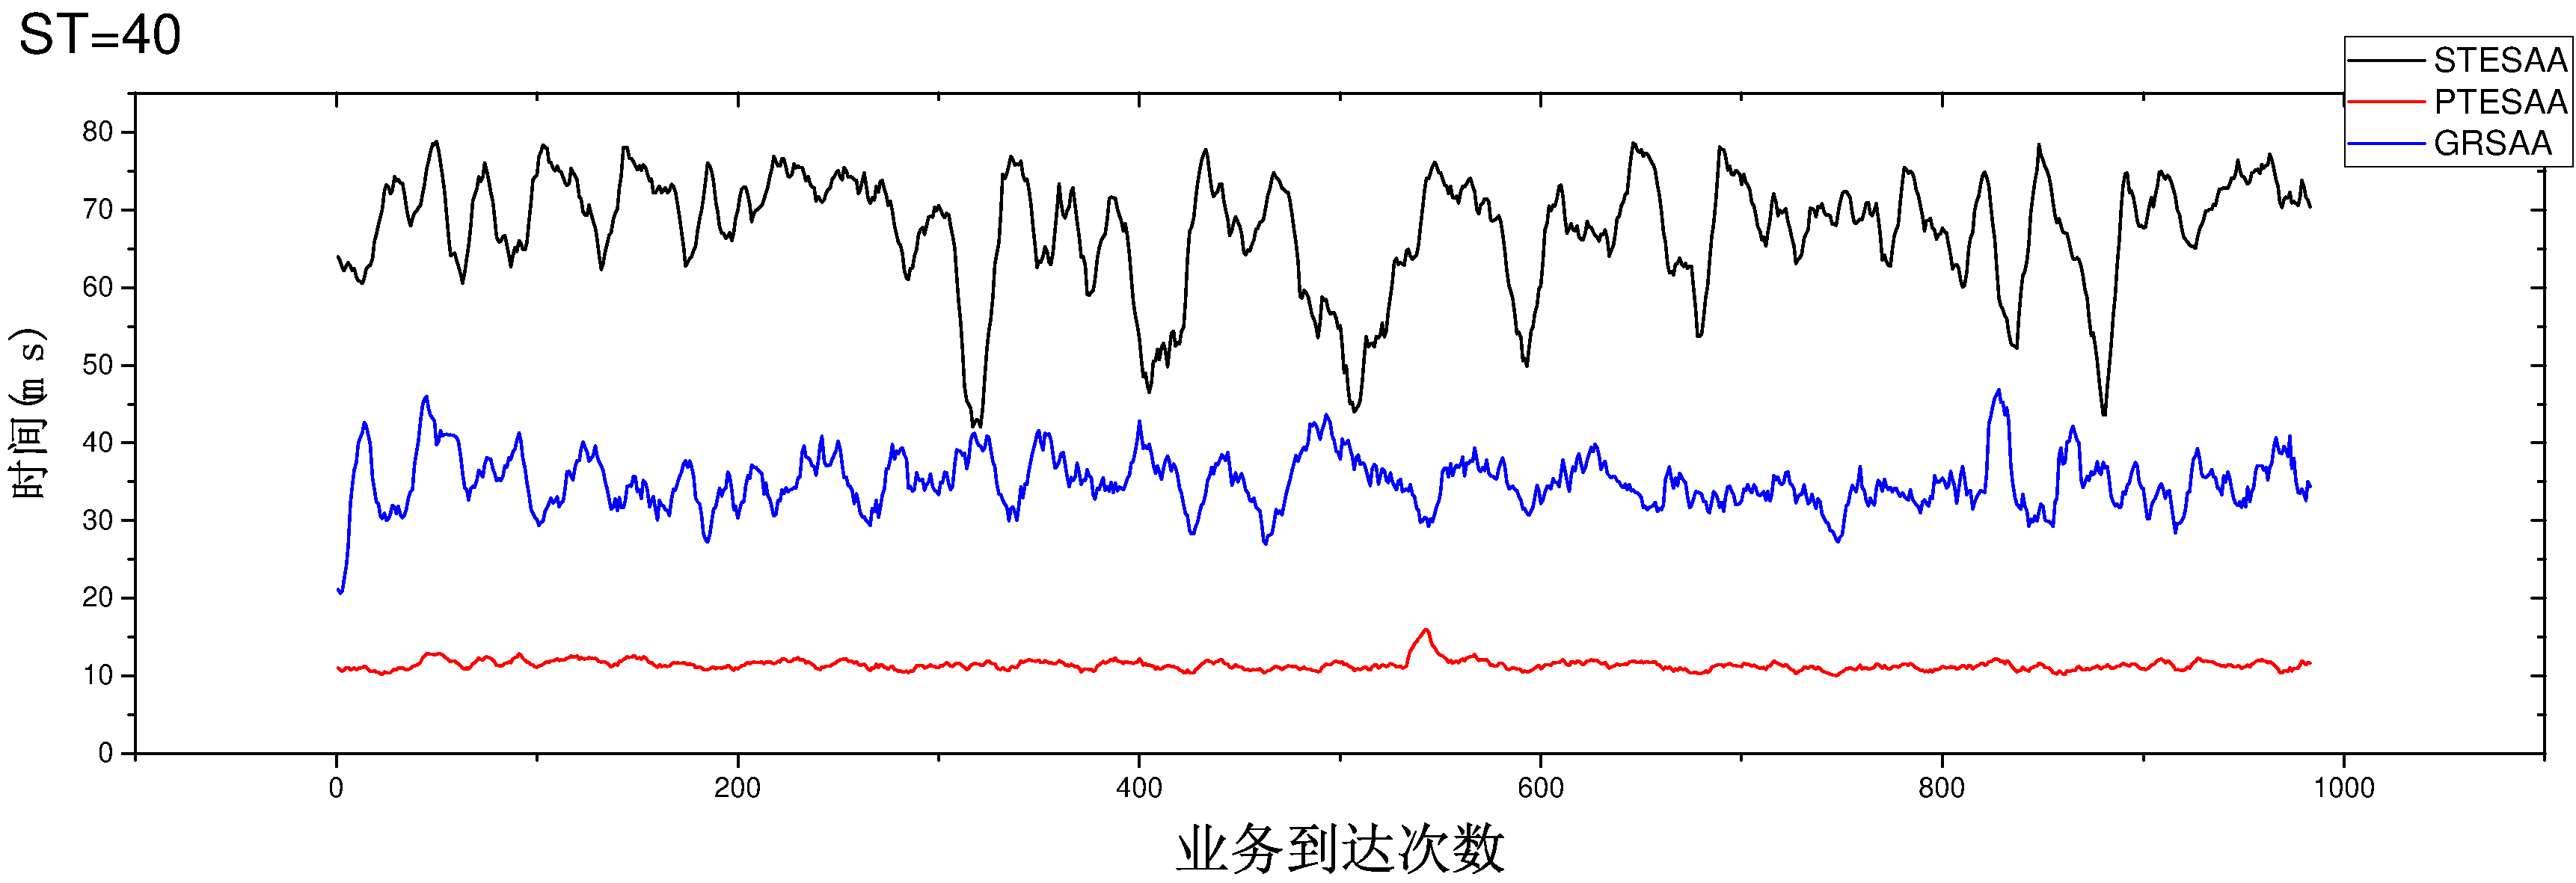
\includegraphics[width=1 \textwidth]{figures/B40T.pdf}}
\end{center}
\caption{{\footnotesize{无权图时间对比(ST=40)}}}
\label{B40T}
\end{figure*}

\begin{figure*}
\setlength{\abovecaptionskip}{-0.5cm}
\begin{center}
{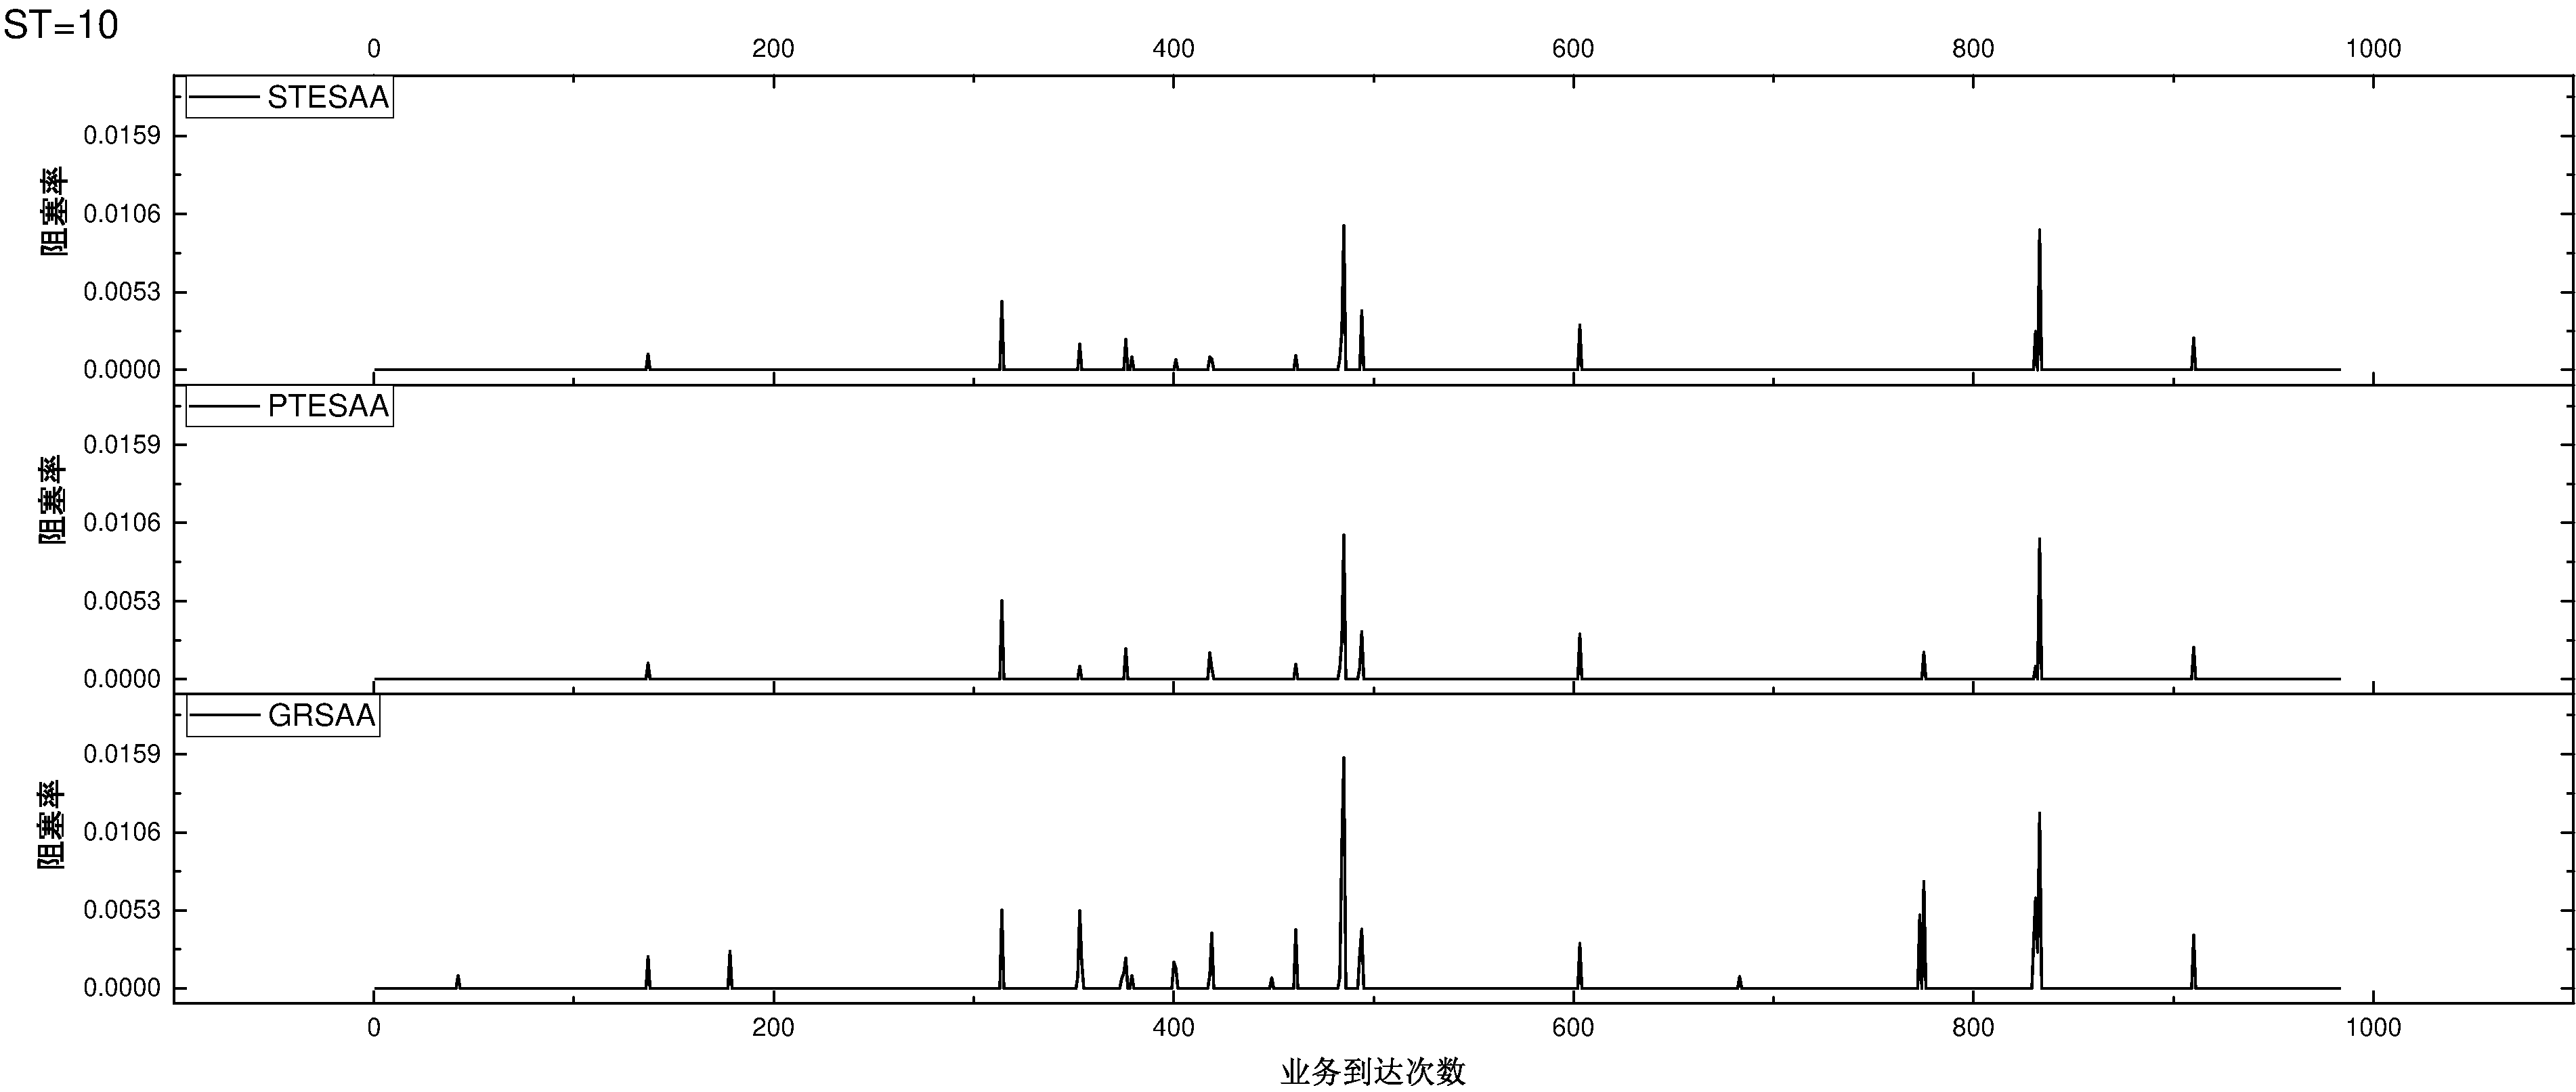
\includegraphics[width=1 \textwidth]{figures/B10Z.pdf}}
\end{center}
\caption{{\footnotesize{无权图阻塞率对比(ST=10)}}}
\label{B10Z}
\end{figure*}
\begin{figure*}
\setlength{\abovecaptionskip}{-0.5cm}
\begin{center}
{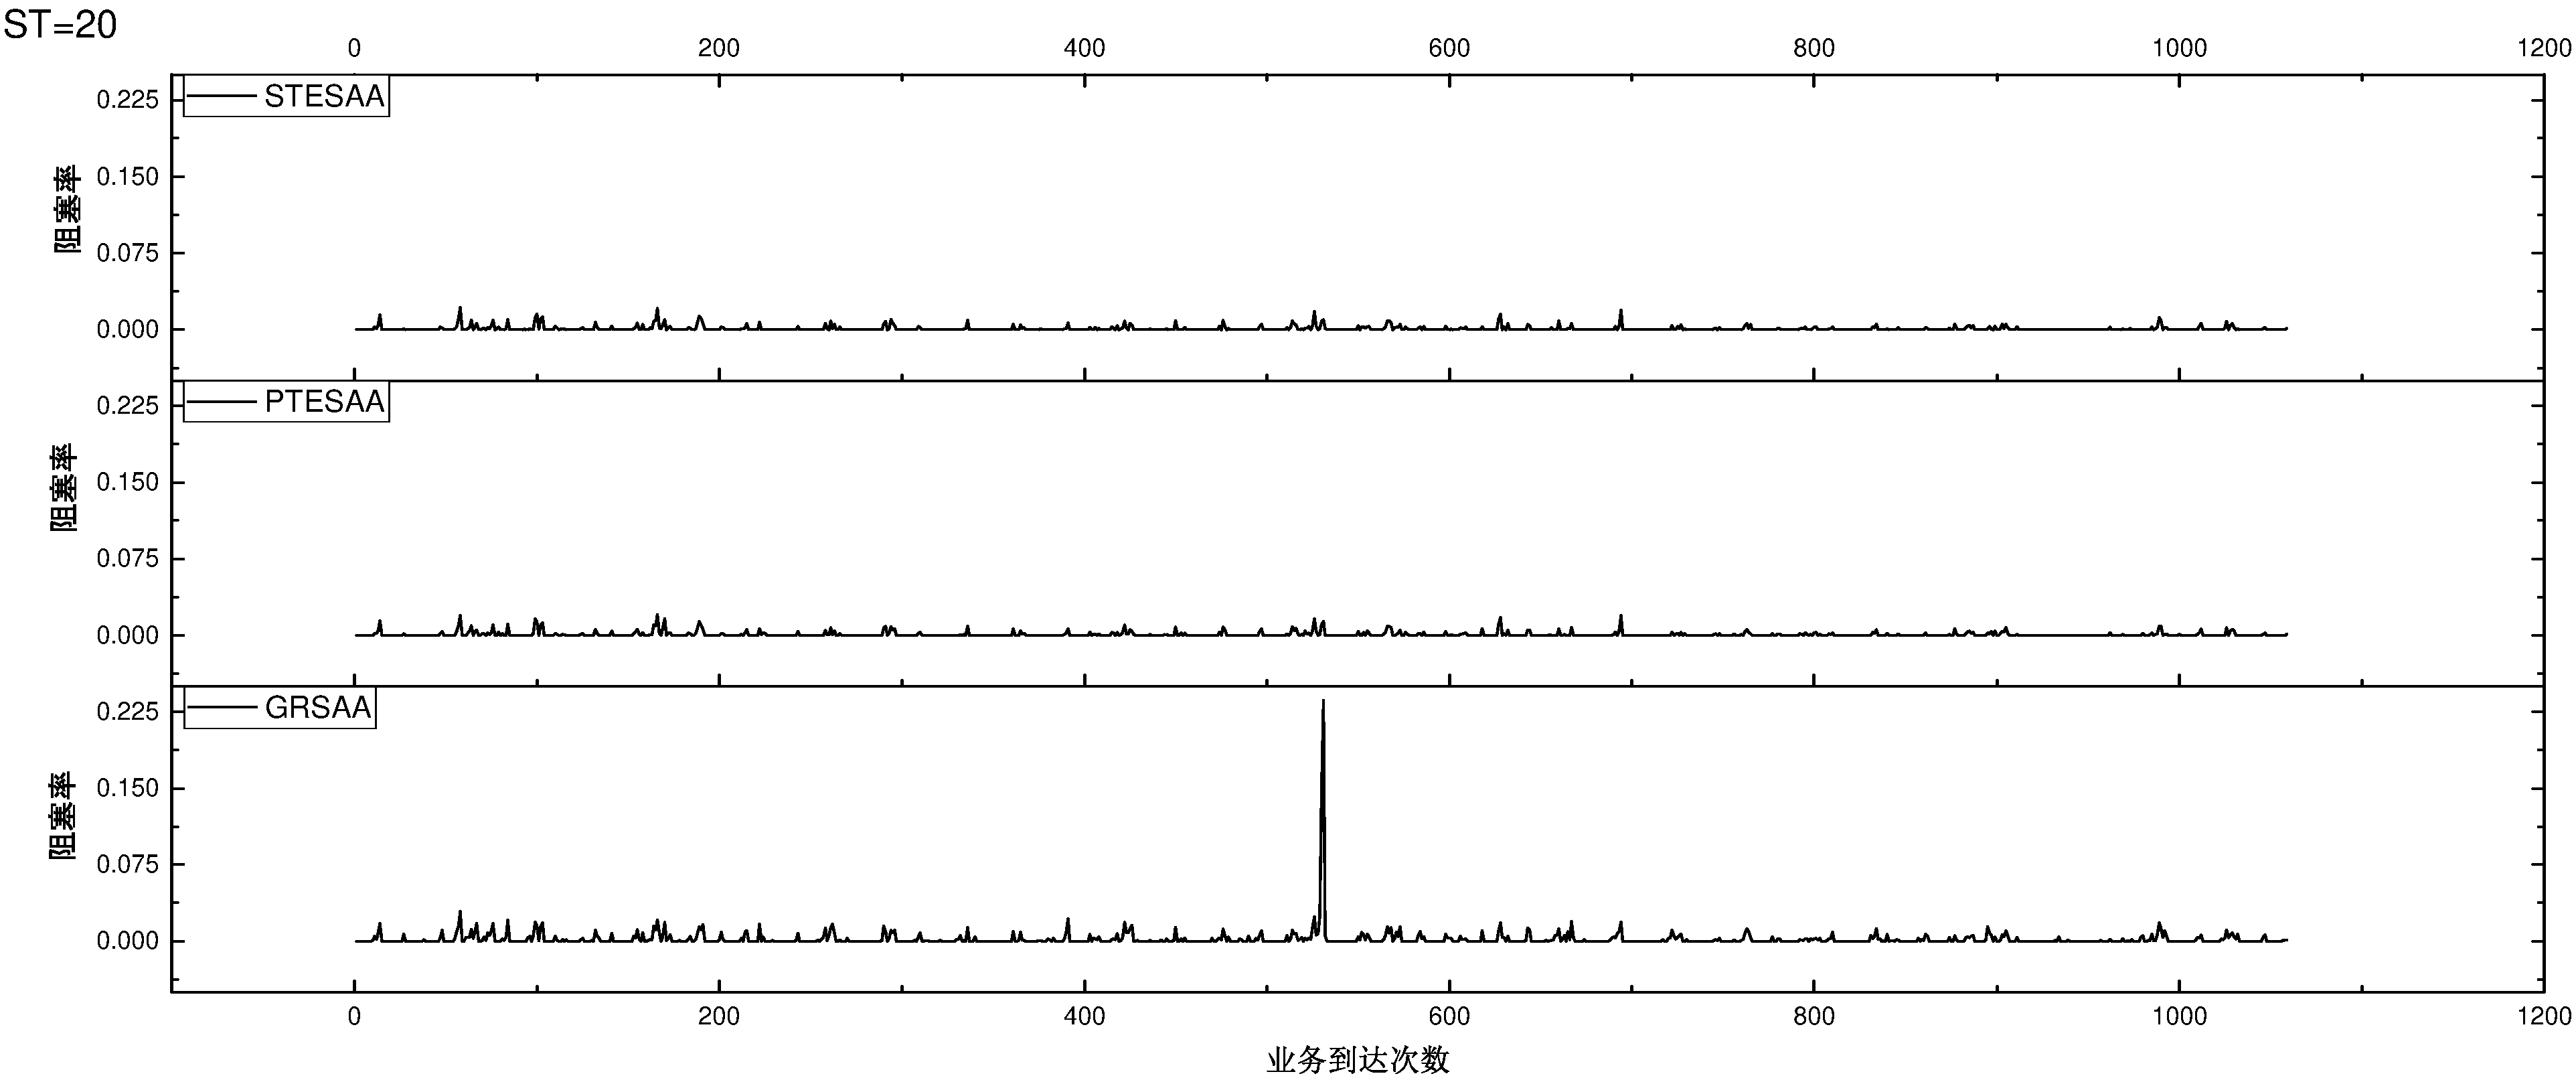
\includegraphics[width=1 \textwidth]{figures/B20Z.pdf}}
\end{center}
\caption{{\footnotesize{无权图阻塞率对比(ST=20)}}}
\label{B20Z}
\end{figure*}
\begin{figure*}
\setlength{\abovecaptionskip}{-0.5cm}
\begin{center}
{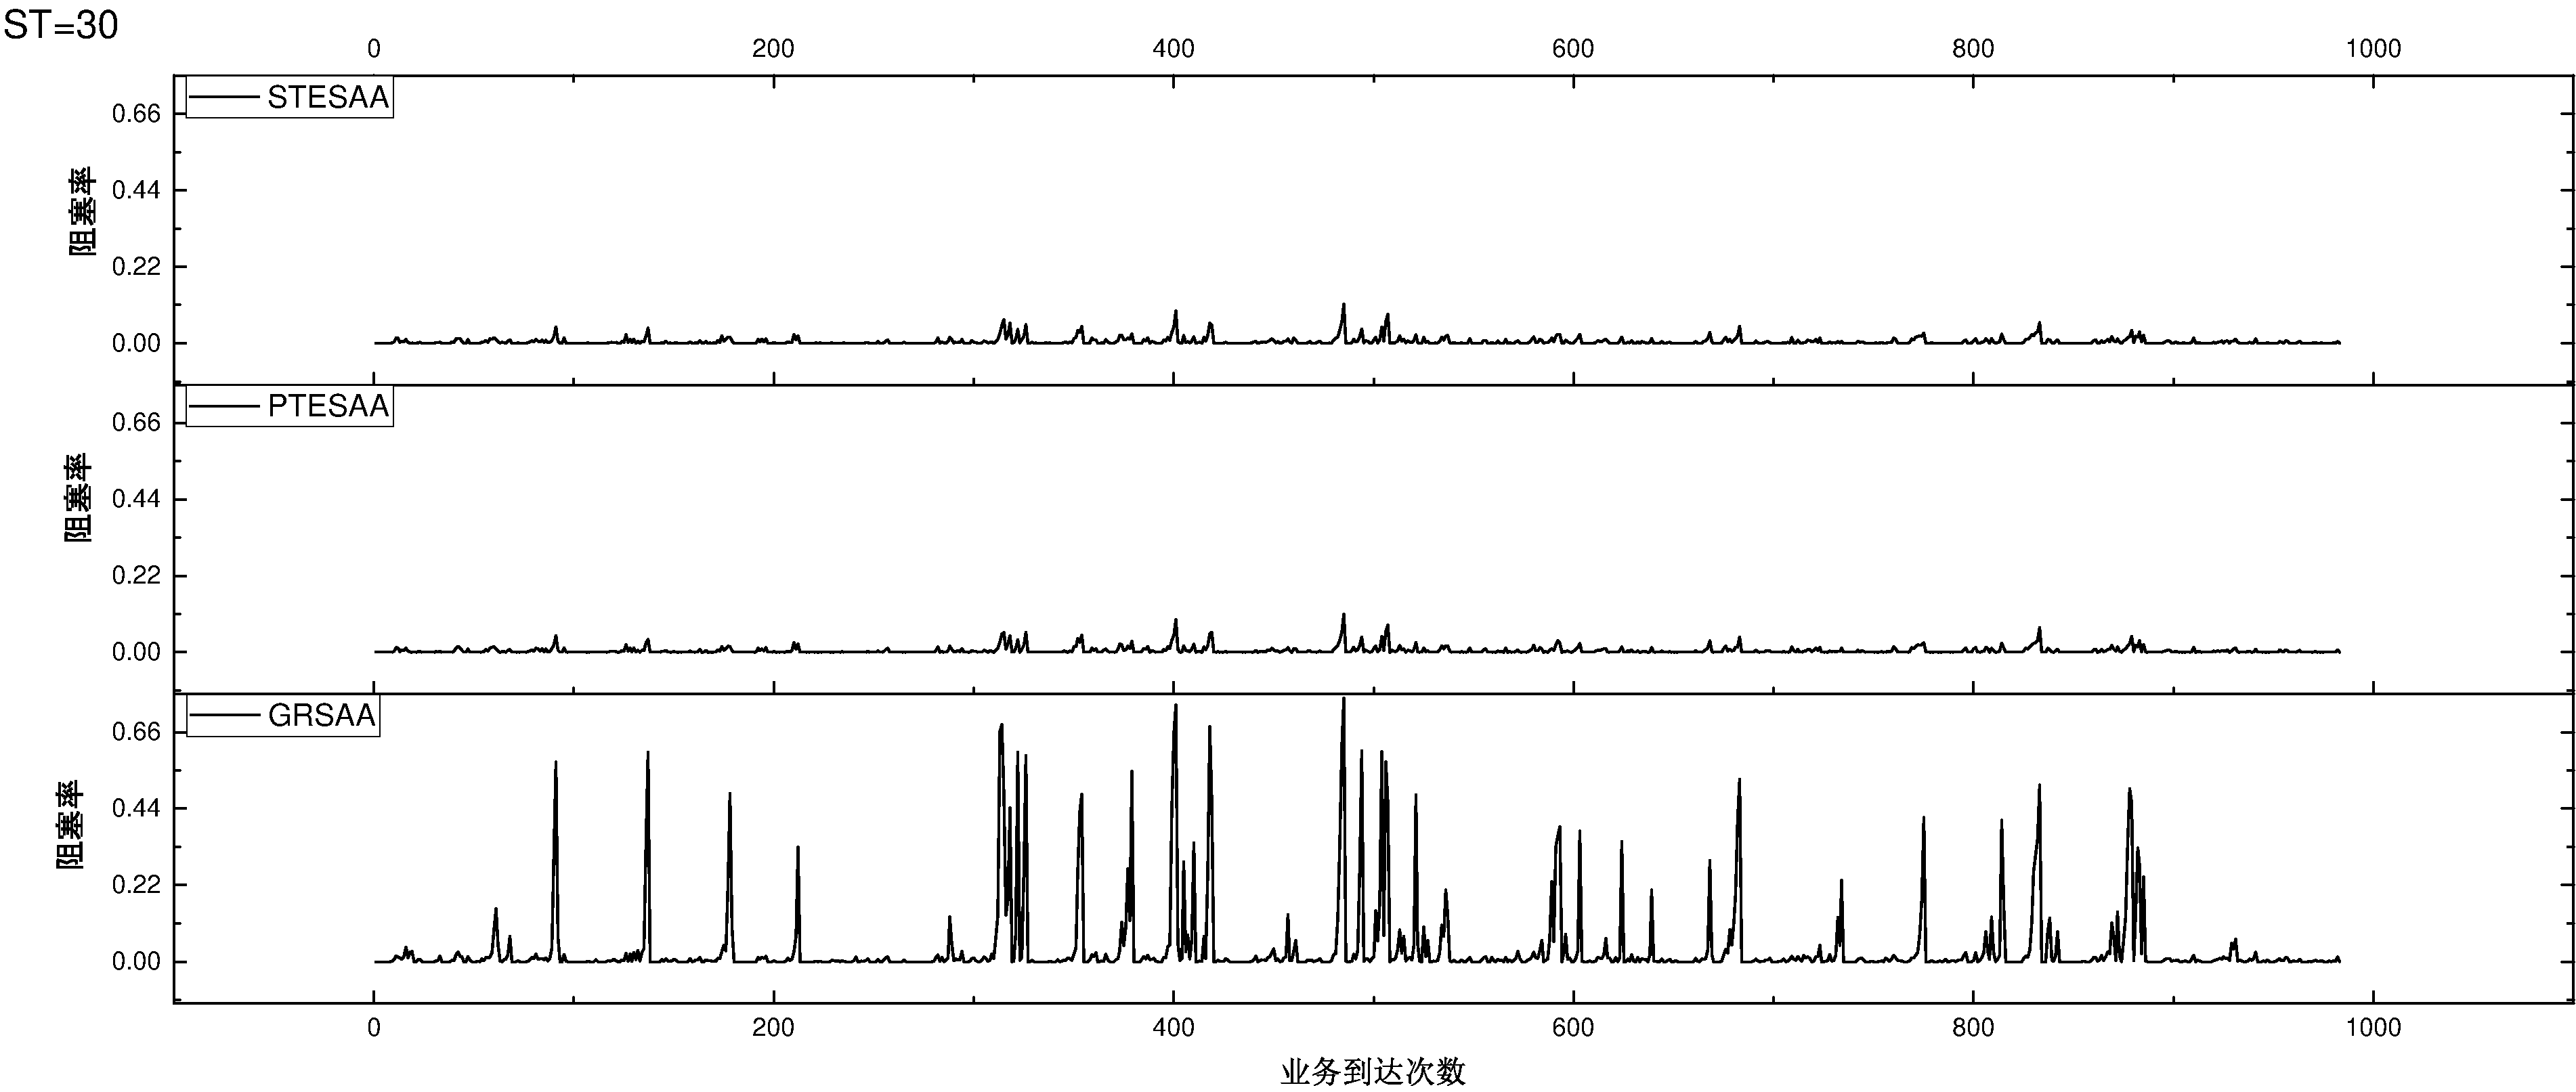
\includegraphics[width=1 \textwidth]{figures/B30Z.pdf}}
\end{center}
\caption{{\footnotesize{无权图阻塞率对比(ST=30)}}}
\label{B40Z}
\end{figure*}
\begin{figure*}
\setlength{\abovecaptionskip}{-0.5cm}
\begin{center}
{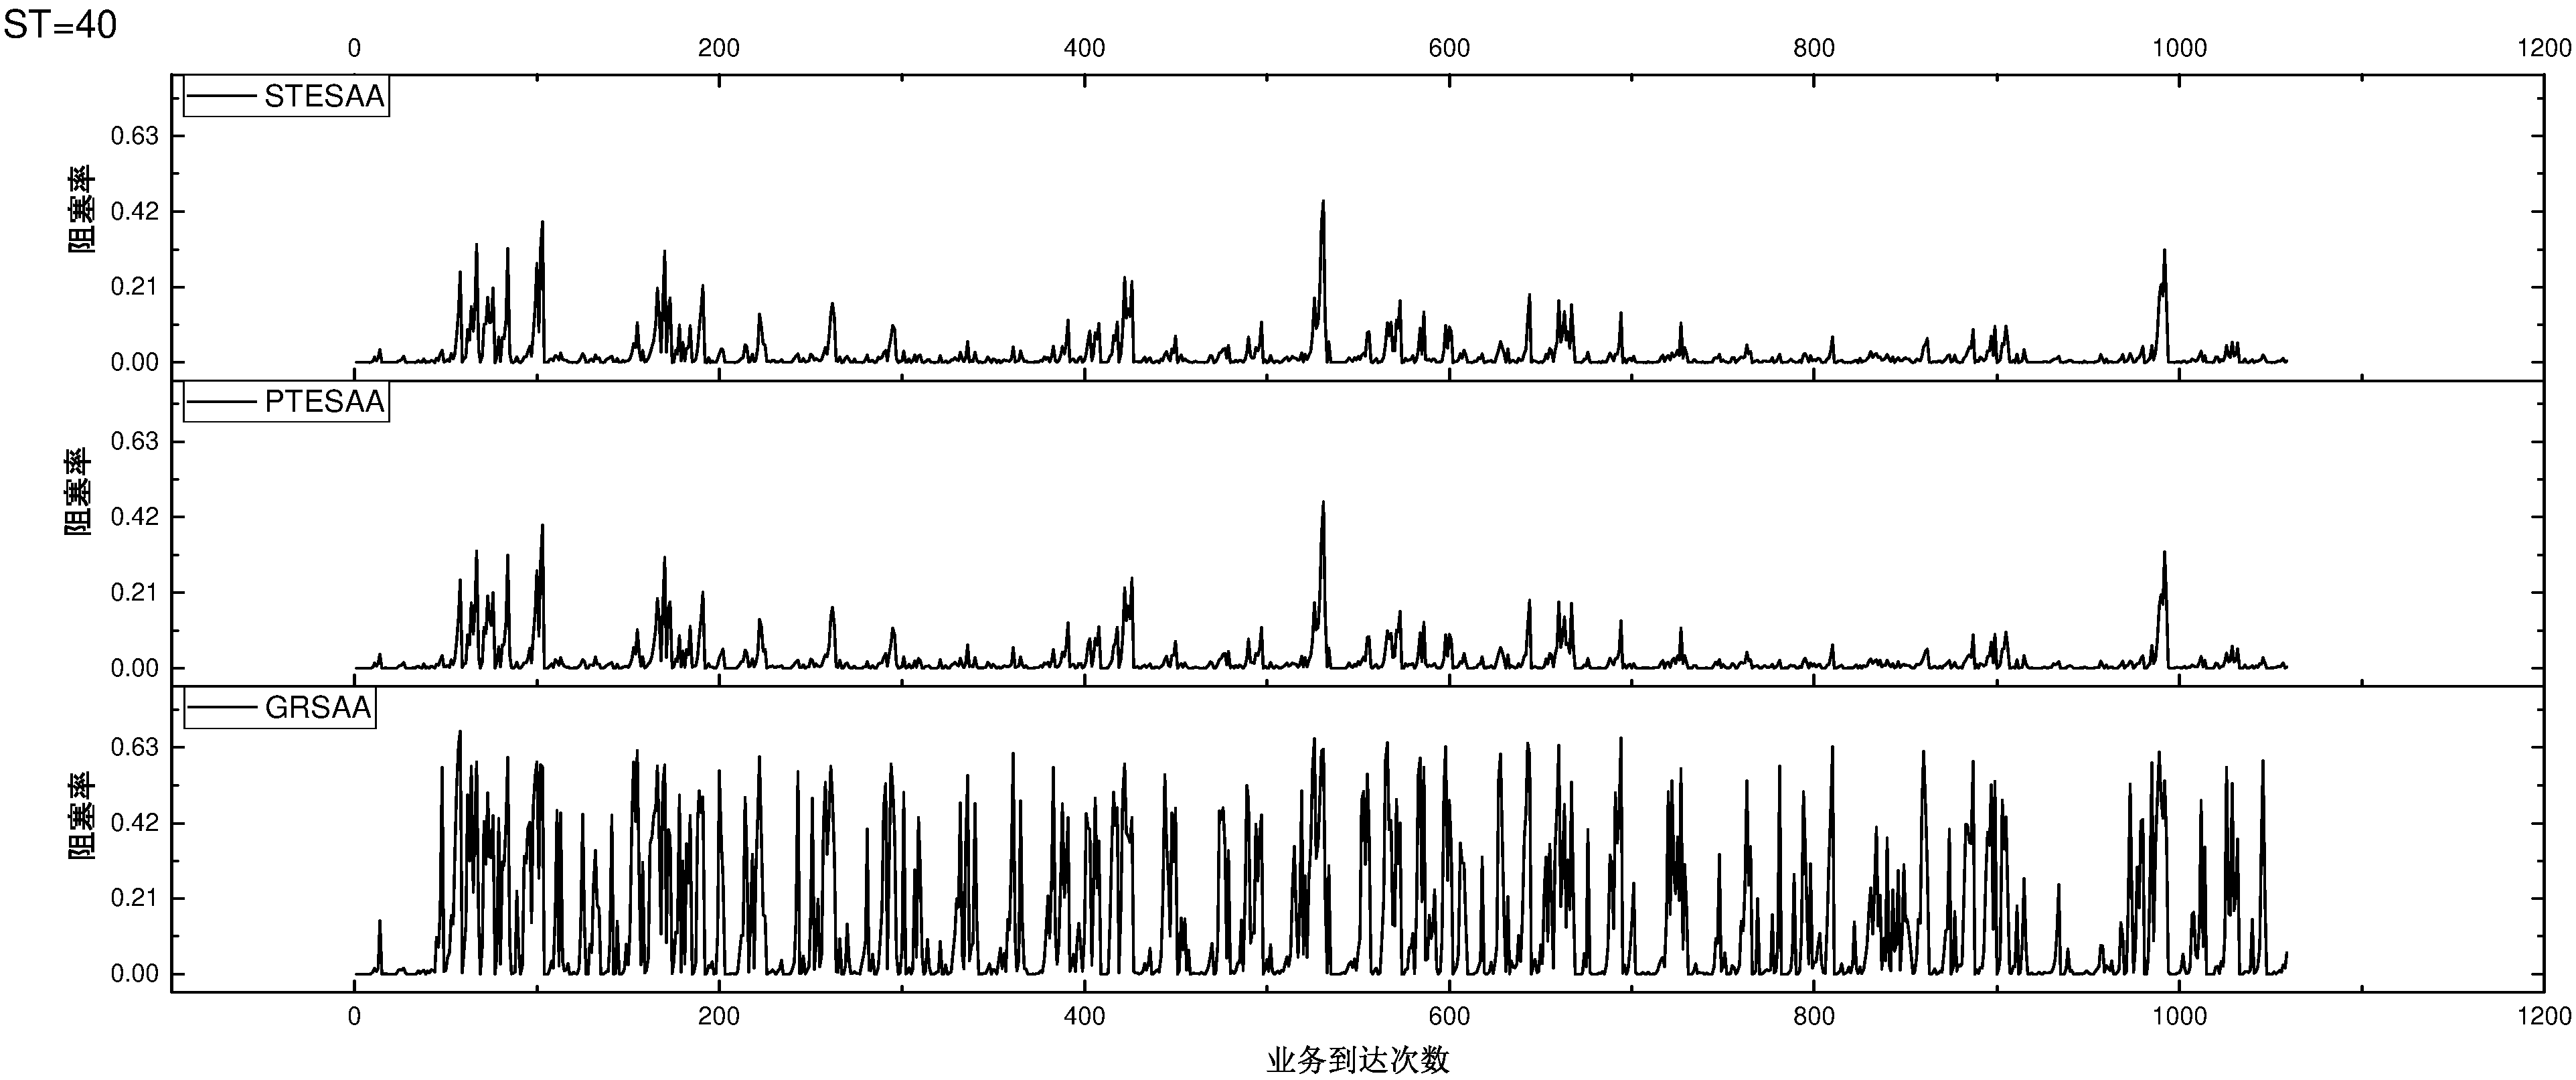
\includegraphics[width=1 \textwidth]{figures/B40Z.pdf}}
\end{center}
\caption{{\footnotesize{无权图阻塞率对比(ST=40)}}}
\label{B40Z}
\end{figure*}

\begin{figure*}
\vspace{-0.5cm}
\setlength{\abovecaptionskip}{-0.5cm}
\begin{center}
{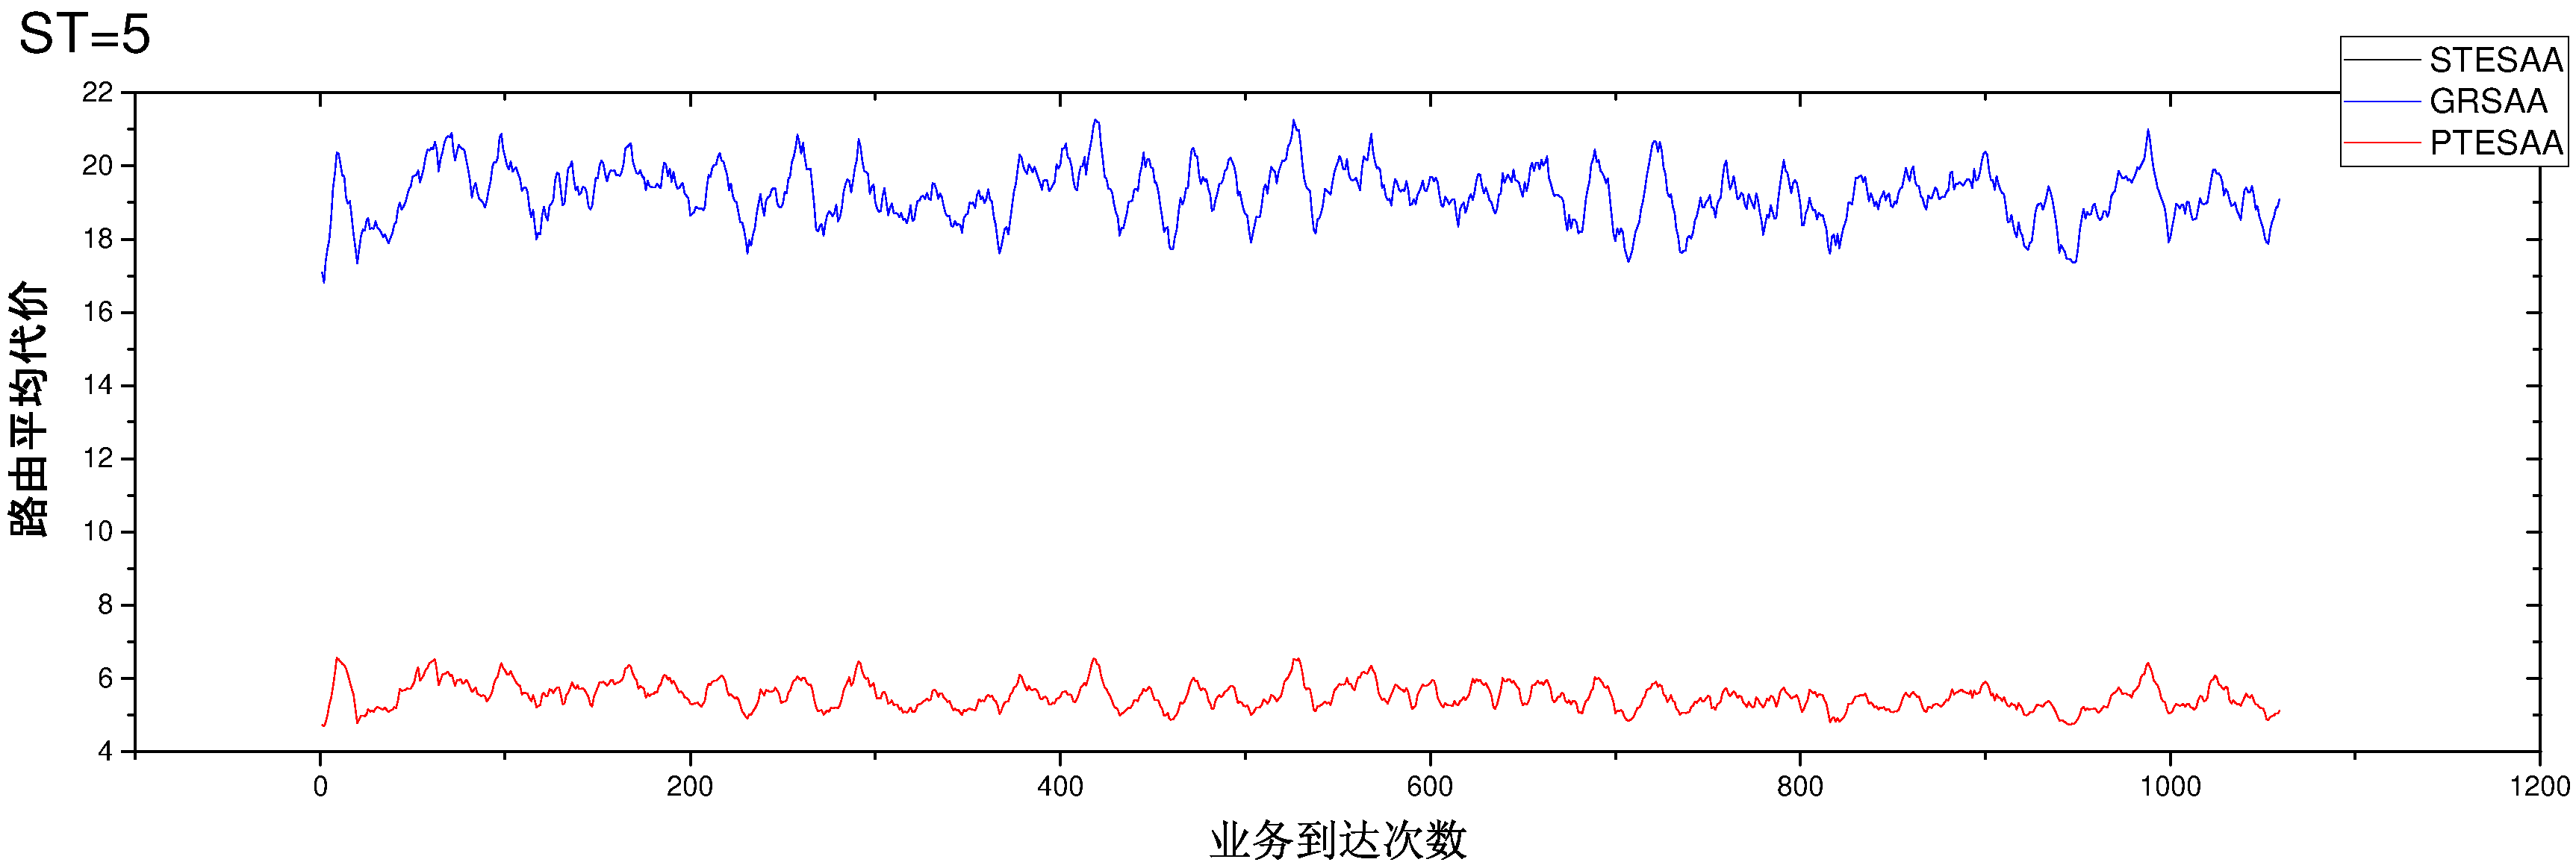
\includegraphics[width=1 \textwidth]{figures/H5C.pdf}}
\end{center}
\caption{{\footnotesize{带权图路由代价对比(ST=5)}}}
\label{H5C}
\end{figure*}
\begin{figure*}
\vspace{-0.5cm}
\setlength{\abovecaptionskip}{-0.5cm}
\begin{center}
{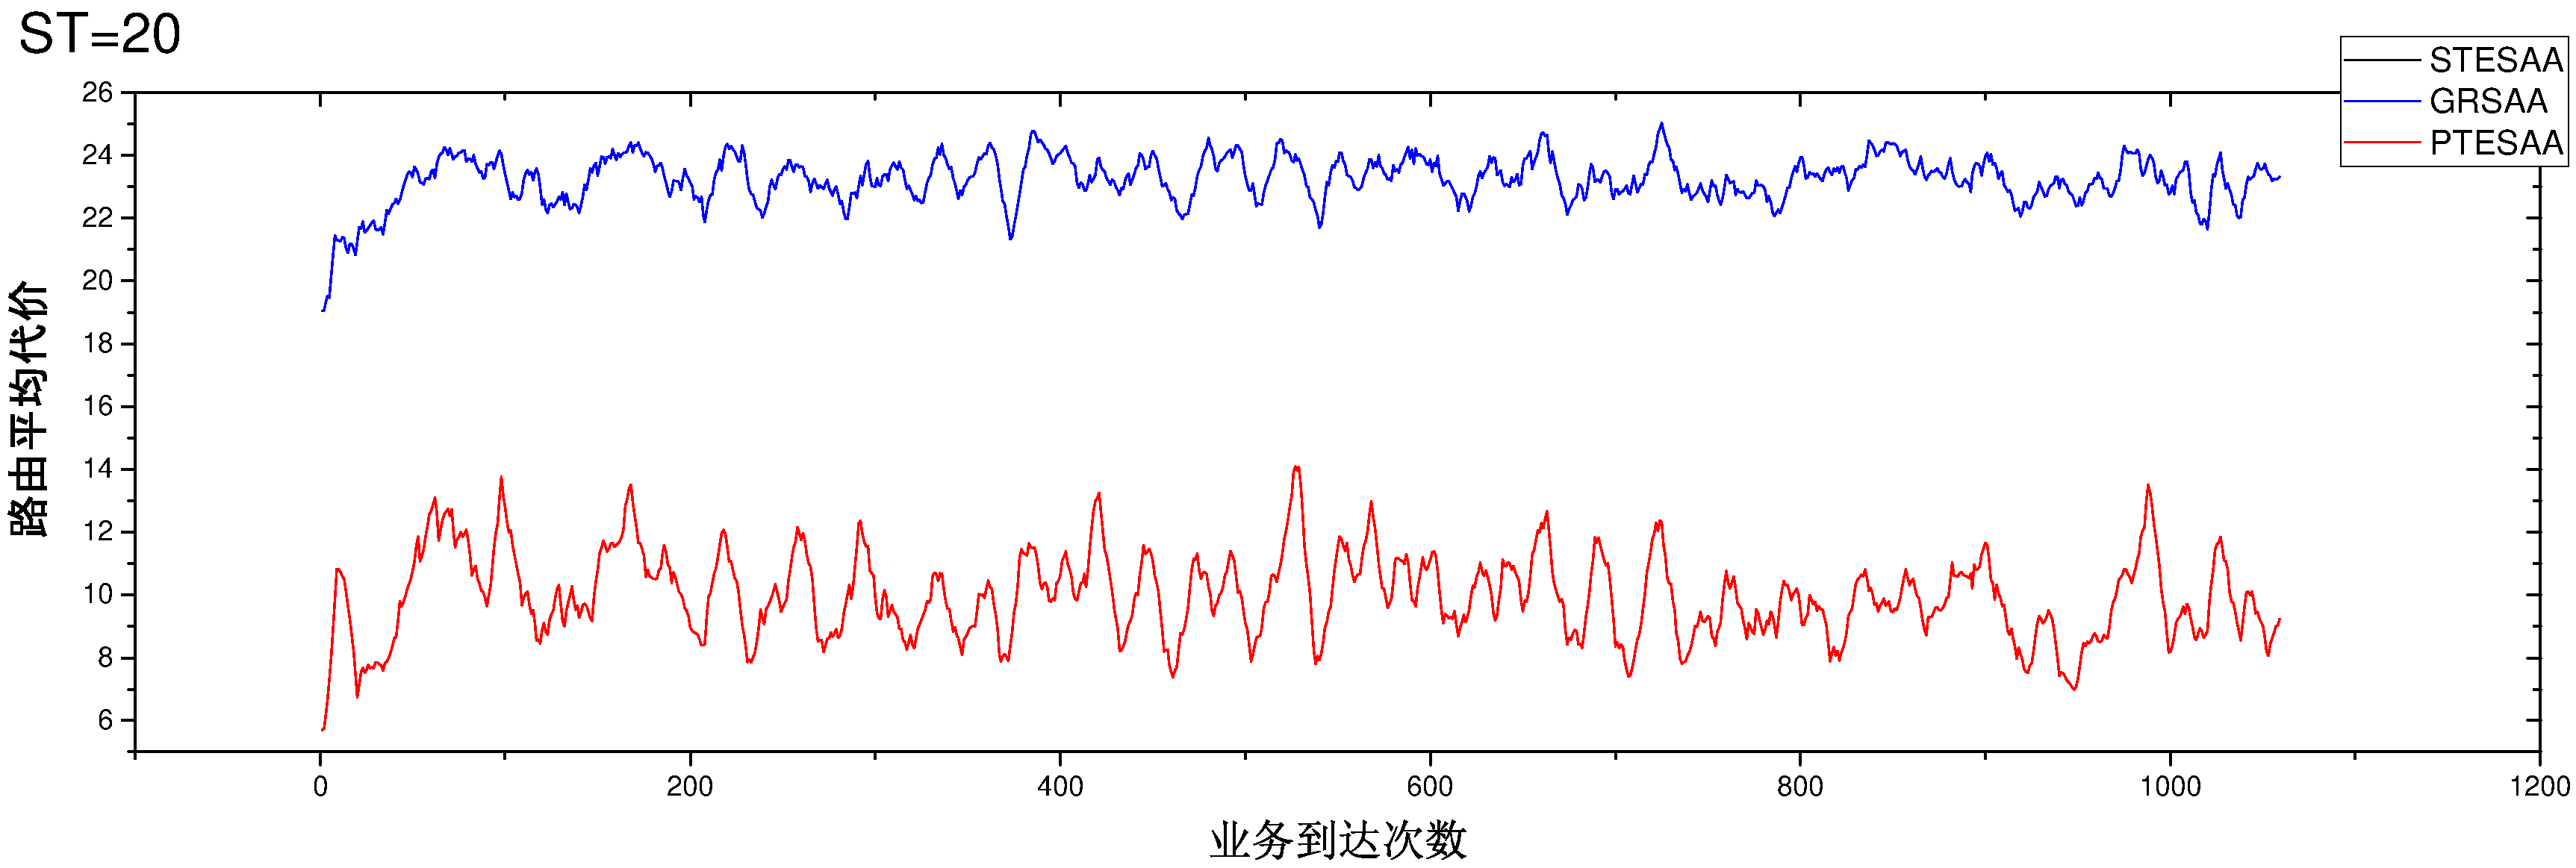
\includegraphics[width=1 \textwidth]{figures/H20C.pdf}}
\end{center}
\caption{{\footnotesize{带权图路由代价对比(ST=20)}}}
\label{H20C}
\end{figure*}
\begin{figure*}
\vspace{-0.5cm}
\setlength{\abovecaptionskip}{-0.5cm}
\begin{center}
{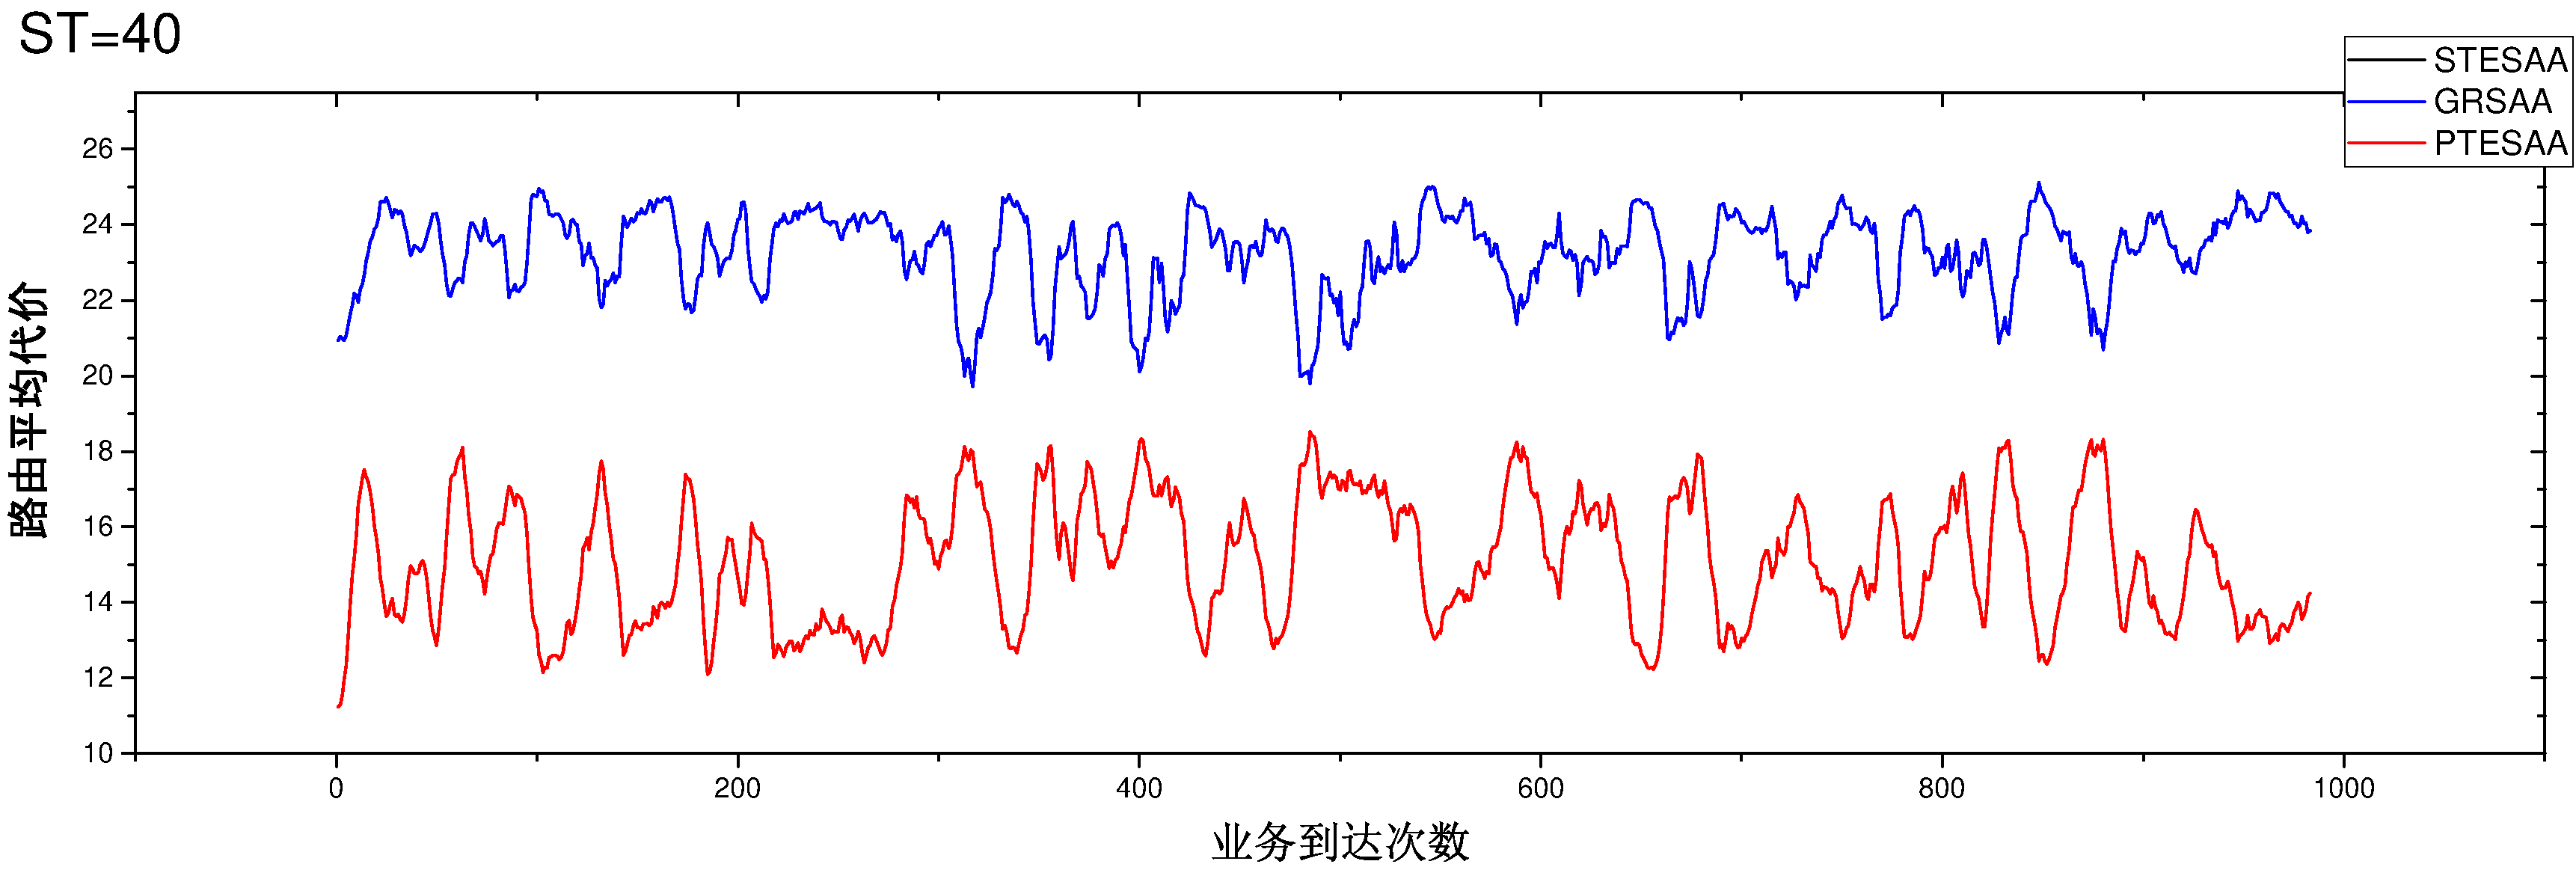
\includegraphics[width=1 \textwidth]{figures/H40C.pdf}}
\end{center}
\caption{{\footnotesize{带权图路由代价对比(ST=40)}}}
\label{H40C}
\end{figure*}
\begin{figure*}
\vspace{-0.5cm}
\setlength{\abovecaptionskip}{-0.5cm}
\begin{center}
{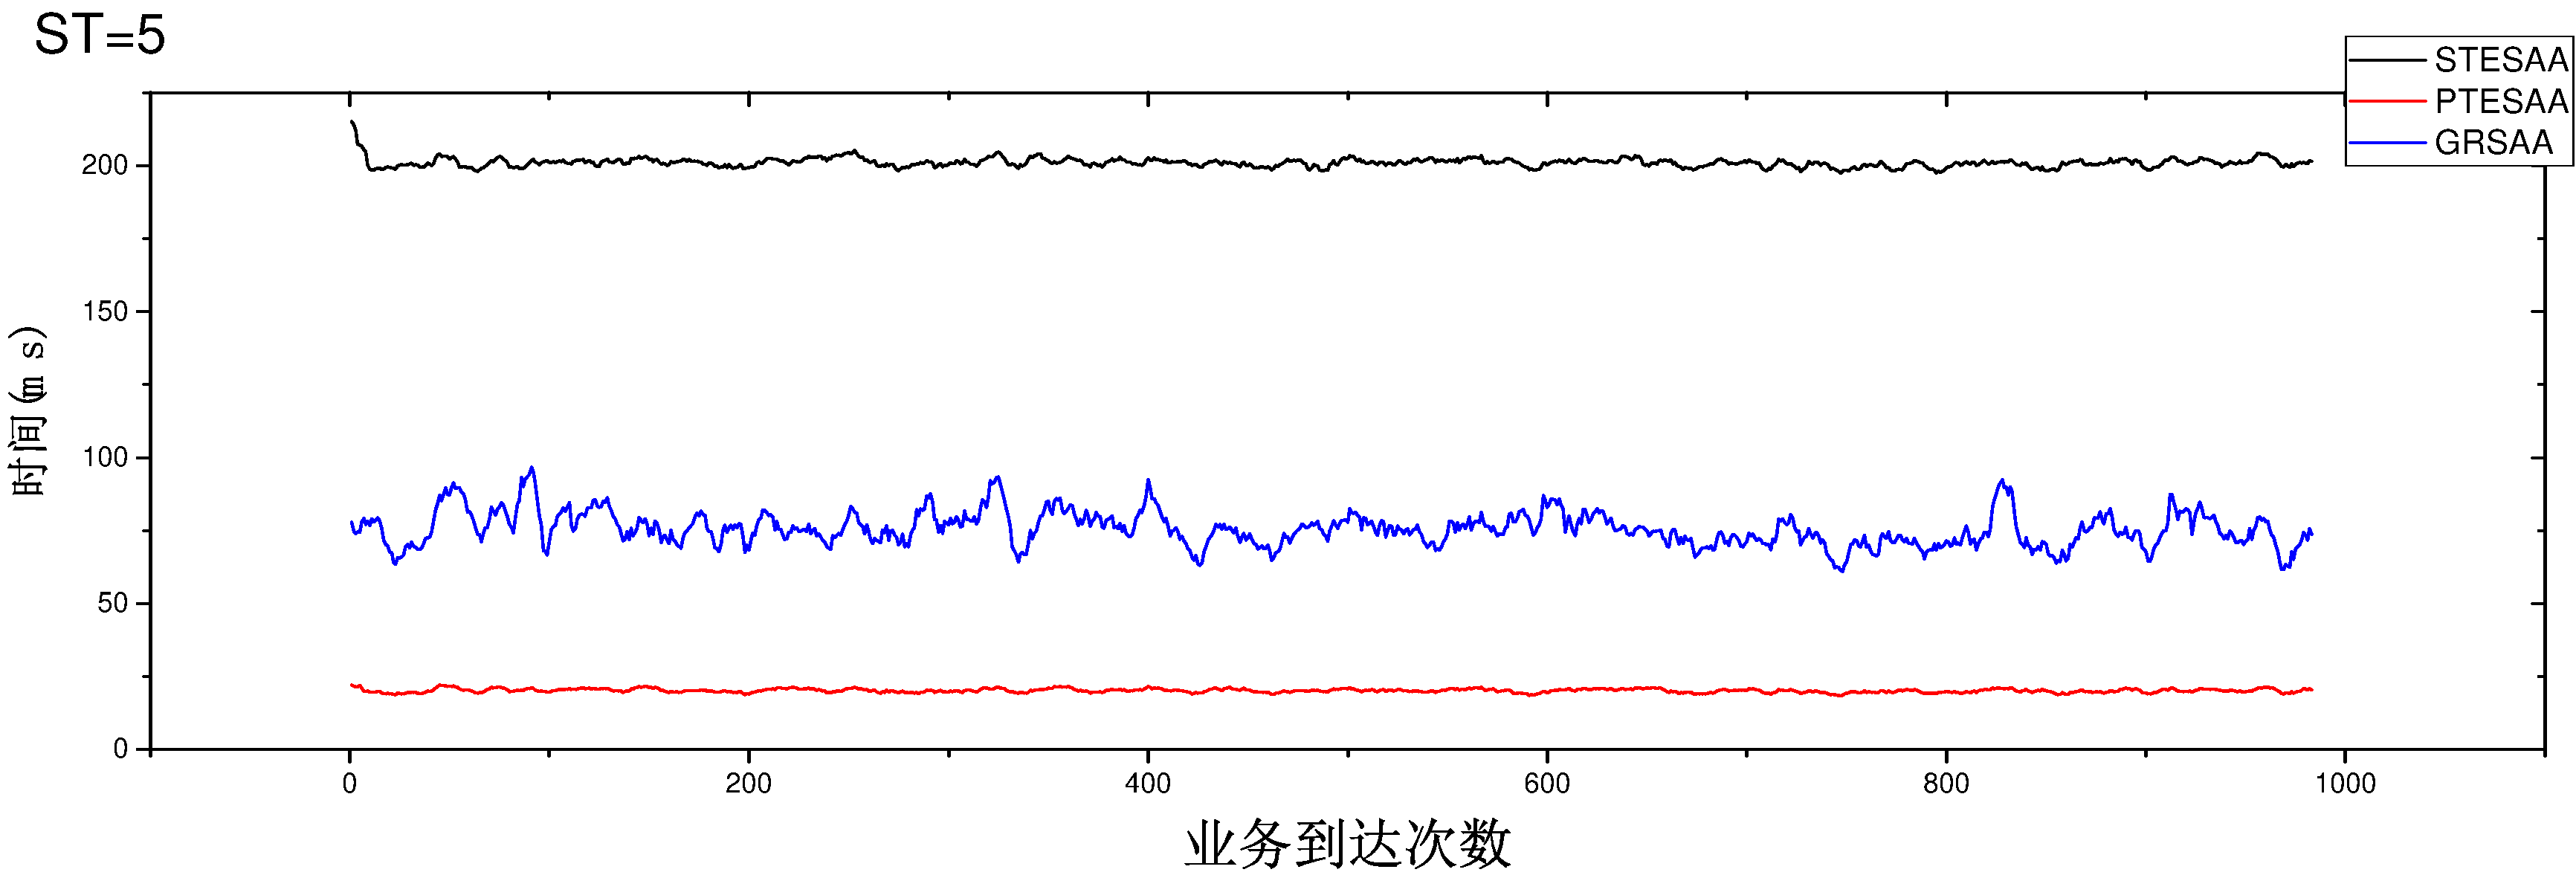
\includegraphics[width=1 \textwidth]{figures/H5T.pdf}}
\end{center}
\caption{{\footnotesize{带权图时间对比(ST=5)}}}
\label{H5T}
\end{figure*}
\begin{figure*}
\vspace{-0.5cm}
\setlength{\abovecaptionskip}{-0.5cm}
\begin{center}
{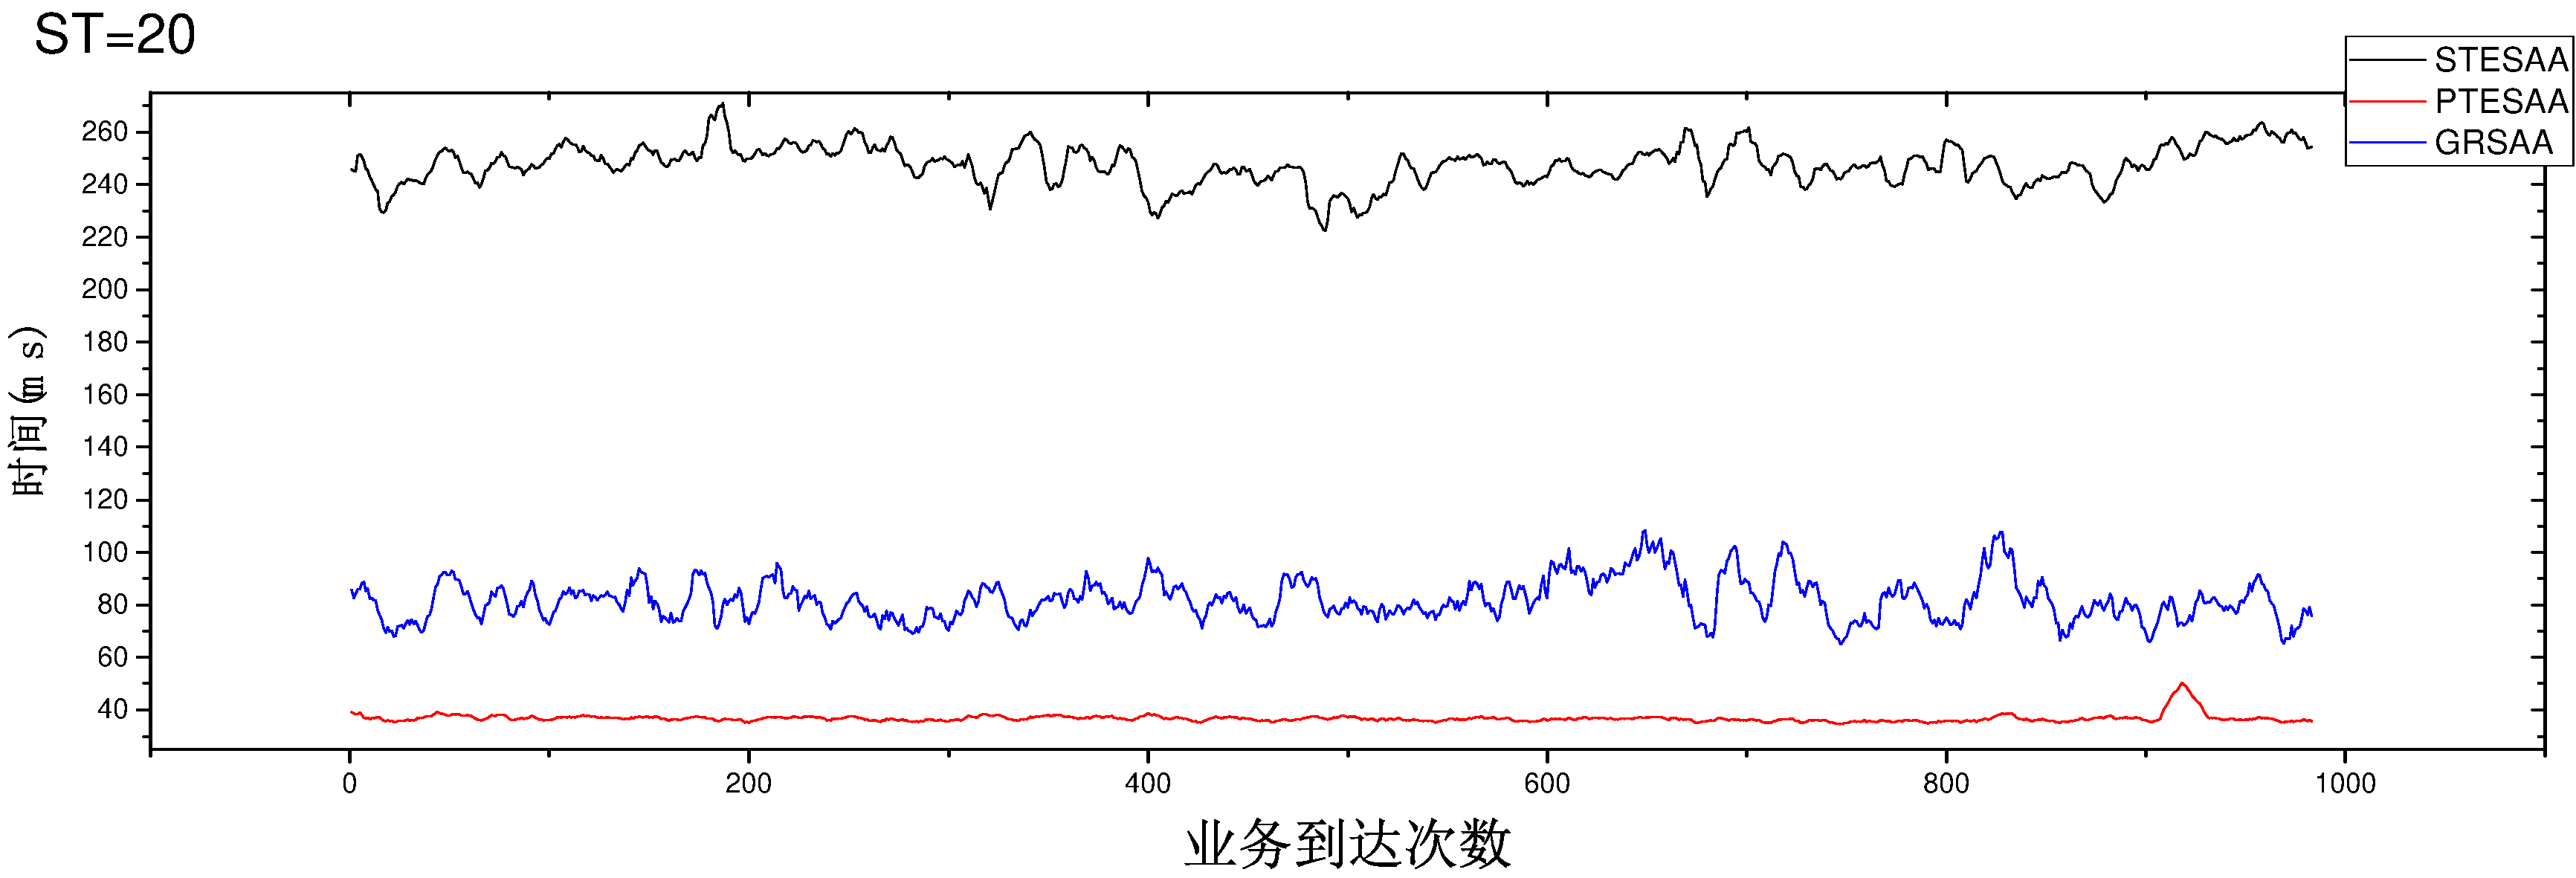
\includegraphics[width=1 \textwidth]{figures/H20T.pdf}}
\end{center}
\caption{{\footnotesize{带权图时间对比(ST=20)}}}
\label{H20T}
\end{figure*}
\begin{figure*}
\vspace{-0.5cm}
\setlength{\abovecaptionskip}{-0.5cm}
\begin{center}
\vspace{-0.05cm}
{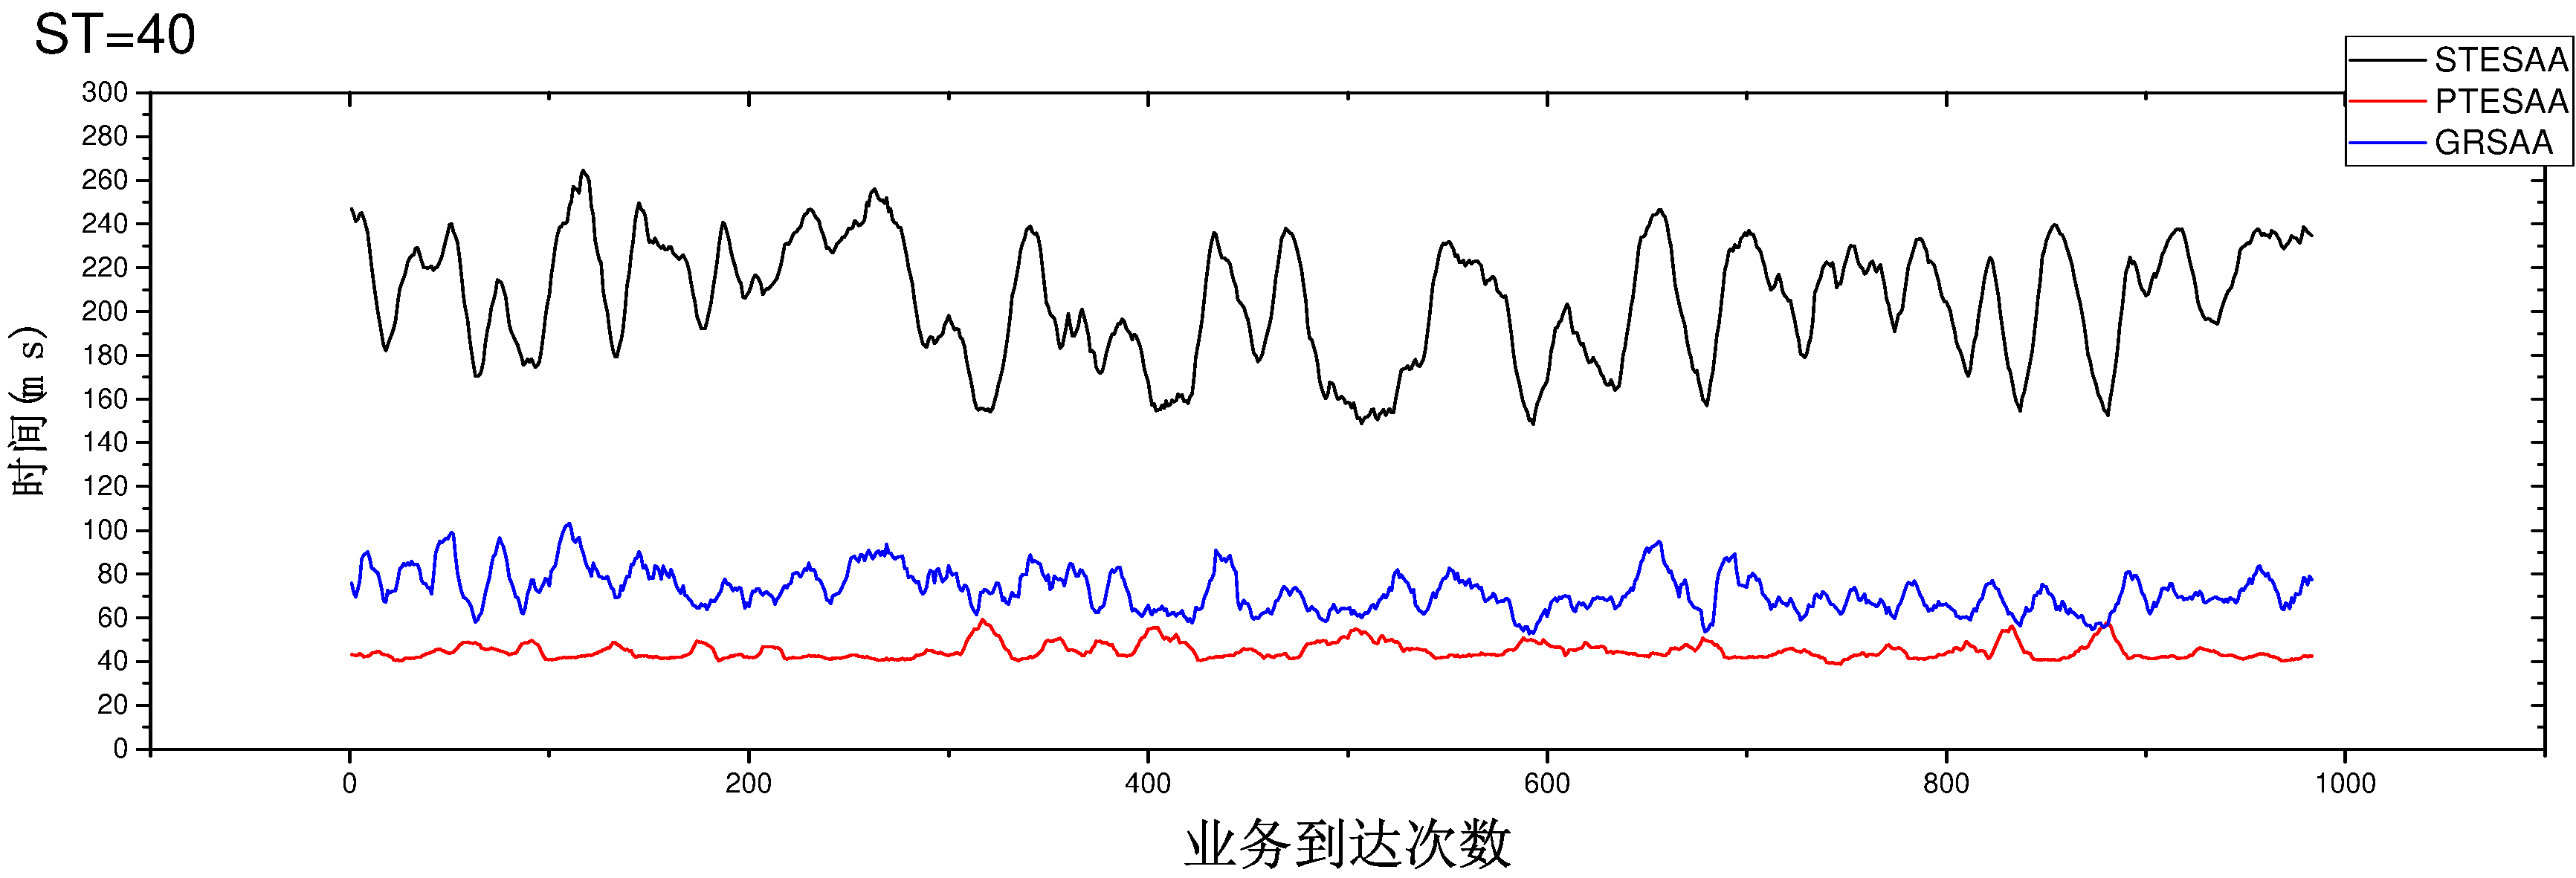
\includegraphics[width=1 \textwidth]{figures/H40T.pdf}}
\end{center}
\caption{{\footnotesize{带权图时间对比(ST=40)}}}
\label{H40T}
\end{figure*}

\subsection{带权图下的仿真结果}
\subsubsection{路由代价优化结果分析}
带权图情况下我们把网络中每条链路的权值设置为1到10之间的随机整数值。图 \ref{H5C}和图 \ref{H40C}表示了路由代价的优化结果,我们把PTESAA和STESAA的优化结果与贪心算法GRSAA的结果进行比较,图中的横坐标表示业务到达的次数,纵坐标表示业务路由的平均代价。

当网络状况较好的时候,比如,平均服务时间为$ST=5$时,如图\ref{H5C}所示,算法PTESAA/STESAA得到的平均路由代价大约为GRSAA得到的平均路由代价的3到4分之一,路由代价得到很大优化。

当网络较拥塞时,比如,平均服务时间为$ST=40$时,如图\ref{H40C}所示,由于网络中的可用链路变少,业务的路径选择空间变小,使得业务可能会选择代价较大的路径进行路由,所以PTESAA/STESAA算法得到的平均路由代价变大,但是PTESAA/STESAA的平均路由代价依然比GRSAA的平均路由代价小很多。

\subsubsection{时间分析}
图 \ref{H5T}到图 \ref{H40T}展示了带权图中各个算法在不同平均服务时间$ST$下的计算时间,当$ST=5$时,我们可以看到PTESAA的计算时间是STESAA的计算时间的1/4,和无权图下PTESAA算法的计算一样,带权图下的PTESAA计算中步骤一的GPU加速比也可达到7-8倍,但是由于步骤二的计算时间不可忽略,使得总体加速比降为4-5倍。

观察图\ref{H5T}到图\ref{H40T},我们发现带权图下的PTESAA/STESAA的计算时间依然优于GRSAA的计算时间。另外,随着网络拥塞程度的增加,可用链路变少,PTESAA对STESAA的加速比略有下降。
\begin{figure*}
\setlength{\abovecaptionskip}{-0.5cm}
\begin{center}
{\includegraphics[width=0.8 \textwidth]{figures/H30Z.pdf}}
\end{center}
\caption{{\footnotesize{带权图阻塞率对比(ST=30)}}}
\label{H30Z}
\end{figure*}



\subsubsection{阻塞率分析}
虽然在带权图中,TESAA目标是去优化路由代价,而并不是去优化路由跳数,但是路由代价较小也在一定程度上意味着路由的跳数较小。所以在带权图中,PTESAA/STESAA求得的路径跳数也比较小,使用的链路资源较少,从而也能优化阻塞率。如图\ref{H30Z}和图\ref{H40Z}所示,带权图下的PTESAA/STESAA算法的阻塞率依然比GRSAA的阻塞率小很多。



\section{本章总结}
本章首先讨论了EON中的RSA问题,介绍了分层图模型,针对分层图模型设计了TESAA算法框架,对框架中路由计算部分进行了并行设计,分别在无权图和带权图两种情况下设计了基于GPU的并行算法,实验发现TESAA能够优化路径跳数,路径代价和阻塞率,同时,并行算法PTESAA对串行算法STESAA的加速比能达到5倍。
\begin{figure*}
\setlength{\abovecaptionskip}{-0.5cm}
\begin{center}
{\includegraphics[width=0.8 \textwidth]{figures/H40Z.pdf}}
\end{center}
\caption{{\footnotesize{带权图阻塞率对比(ST=40)}}}
\label{H40Z}
\end{figure*}
\chapter{全文总结与展望}
\section{全文总结}
本文主要研究了SDN网络下适合于并行计算的业务量工程算法框架,并且针对这些框架,设计基于GPU的并行算法。

本文首先简要介绍了GPU的并行优化原理,主要包括GPU与CPU的区别,GPU的架构特点和CUDA编程模式。

第三章在SDN IP网络中,本文将业务量工程问题建模成一个带链路容量约束的以路由代价为目标的MILP模型,为了解决这个MILP模型。本文提出了GA-PTEA和LR-PTEA两种基于GPU的并行算法,并对两种算法的GPU并行设计细节进行了讨论。并行算法GA-PTEA的加速比虽然可以达到15倍,但是由于遗传算法收敛缓慢的原因,其时间表现并不理想。另外由于遗传算法容易陷入局部最优解,所以GA-PTEA求得的解比较差。LR-PTEA能够在短时间内得到业务量工程模型的优化解,说明拉格朗日松弛方法更加适合解决这种资源分配问题。本文设计的对拉格朗日子问题的并行求解方法,可以被应用到其他的网络优化问题当中,如果将优化问题的约束松弛进目标函数后,原优化问题可以被分解为独立的最短路径问题,我们就可以使用本文类似的并行算法来加速这些子问题的求解。这种类型的问题其实很常见,比如$\alpha$公平问题的对偶子问题,当$\alpha>1$时也是求解一批业务的最短路径。

第四章针对SDN弹性光网络,本文采用分层图模型将频谱分配问题转化为路由选择问题,并且利用分层图之间的独立特性来设计并行的业务量工程算法PTESAA。利用GPU强大的并行计算能力,PTESAA在不同的分层图上搜索路径,在短时间内为业务的路由选择提供了更大的空间,从而优化了业务的路由代价,节省了网络资源的使用,降低了阻塞率。第四章设计的动态规划算法可以在多项式时间复杂度($W_{max}\times|E|$)内解决带跳数约束的最短路径问题,能应用到更多的场景当中。

\section{后续工作展望}
GPU并不擅长分支较多的计算,GPU更加适合加速逻辑简单但计算量很大的任务,而路由算法中计算操作并不多,大部分是逻辑计算,这也是为什么本文中的路由算法只能获得较小加速比的原因。本文只利用了GPU的并行处理能力,而没有充分利用GPU的大规模浮点计算能力,这也是GPU应用在路由算法上的限制。所以在今后的工作中可以挖掘更多的计算密集型的任务进行GPU加速。

在研究本次毕业设计的过程中,本人除了设计GA-PTEA,LR-PTEA和TESAA算法之外,还针对弹性光网络分层图上的网络流问题进行了基于GPU的并行化研究。本人对预流推进算法进行了并行化的设计并在其中加入跳限约束。但是由于算法逻辑复杂,加速效果并不好,只能在一些特殊情况,比如流很多的情况下才有一定的加速比,所以这部分工作并没有被写进本次设计。后续我将会继续改进这个预流推进算法,希望可以得到好的加速效果。
\thesisacknowledgement
首先我要感谢我的导师王雄老师,感谢他给我的一切。早在论文开题前,王老师就为我确定好了研究方向,使得我不再迷茫,在毕业设计的研究当中,我常常会因为自己的粗心大意和不严谨的做法导致错误而陷入困难当中,而王老师总是能够耐心的对我进行指导和鼓舞,使我重新找到自信去克服困难,而在论文的写作当中,王老师细致入微地分析我的论文,给我提出了宝贵的修改意见。王老师不仅仅是我科研上的导师,还是我精神上的导师,每每想起和王老师一起探讨算法时的场景,我就非常激动,是王老师让我感受到了算法的无穷魅力,让我找到了我人生想要追寻的方向!在生命的旅程中,能够遇到王老师是我一生的幸运,受用不尽,铭记在心。

其次,我要感谢我的父母,每当我遇到困难的时候,我的父母都能给我精神上的鼓舞,让我感受到家的温暖,正是因为有家的坚强后盾,我才能更加坚强的去追寻梦想。

我还要感谢我的同窗好友,感谢潘神在科研上和生活上对我的帮助,感谢兴爷的饭菜,感谢伟神的carry。我还要感谢实习时的同事,感谢老万对我在计算机视觉算法上的指导,感谢博哥对我在日常工作上的指导,感谢华哥对我在CUDA编程上的指导。

\thesisloadbibliography[nocite]{reference}


\end{document}


